\documentclass[11pt]{book}
\usepackage{fullpage}
\usepackage{epsf}
\usepackage{graphicx,epstopdf}	
\usepackage{parallel}
\usepackage{amsmath}
%\pdfoutput = 1 

\usepackage{fontspec}
\usepackage{fontspec}
\setmainfont{Times New Roman}
\usepackage{polyglossia}
\setmainlanguage{english}
\setotherlanguage{greek}
\newfontfamily\greekfont{Times New Roman}

\newcommand {\btau}{\mbox{\boldmath$\tau$}}
\newcommand {\bOmega}{\mbox{\boldmath$\Omega$}}
\newcommand {\bomega}{\mbox{\boldmath$\omega$}}

\includeonly{Introduction/Introduction,Spherical/Spherical}

\begin{document}

\title{{\bf A Modern Almagest}:\\[0.5ex]An Updated  Version of Ptolemy's Model of the Solar System}
\author{Richard Fitzpatrick}
\date{}
\maketitle

\chapter{Introduction} 
% !TEX root = ../Almagest.tex

\section{Euclid's Elements and Ptolemy's Almagest}
The modern world inherited two major scientific treaties from the civilization
of ancient Greece. 
The first of these, the  {\em Elements}\/ (\begin{greek}Στοιχεῖα\end{greek}) of Euclid (\begin{greek}Εὐκλείδης\end{greek}), is a
large compendium of mathematical theorems concerning geometry, proportion, and number
theory. These theorems were not necessarily discovered by Euclid
himself---being largely the work of earlier mathematicians,
such as Eudoxos of Cnidus (\begin{greek}Εὔδοξος ὁ Κνίδιος\end{greek}), and Theaetetus of Athens (\begin{greek}Θεαίτητος ὁ Ἀθηναῖος\end{greek}) ---but were arranged
by him in a logical manner, so as to demonstrate that they can all ultimately
be derived from five simple axioms. The Elements is rightly regarded
as the first, largely successful, attempt to construct an
axiomatic system in mathematics, and is still held in high esteem within
the scientific community.

The second treatise, the {\em Almagest}\,\footnote{The true title
of this work is \begin{greek}Μαθηματικὴ Σύνταξις\end{greek}, which means ``Mathematical Treatise''.  The treatise was later called  \begin{greek}Ἡ Μεγάλη Σύνταξις\end{greek},  meaning ``The Great Treatise'',
and the superlative form of the adjective, \begin{greek}μεγίστη\end{greek},  with the Arabic article ``al" prepended, lies behind the Arabic name from which the English name Almagest derives.} of Claudius Ptolemy (\begin{greek}Κλαύδιος Πτολεμαῖος\end{greek}), 
is an attempt to find a simple geometric explanation for the apparent motions of the Sun,
the Moon, and the five visible planets in the Earth's sky.  On the basis of his own naked-eye observations, combined with those of earlier astronomers such as Hipparchus of Nicaea (\begin{greek}Ἱππάρχος ὁ Νικαεύς\end{greek}), Ptolemy proposed  a model of the Solar System in which the Earth is stationary.
According to this model, the Sun moves in a circular orbit, (nearly) centered on the Earth, that 
maintains a fixed inclination of about $23^\circ$ to the  terrestrial equator.
Furthermore, each planet moves  on the rim of a small
circle called an {\em epicycle}\/ (\begin{greek}ἐπίκυκλος\end{greek} in Greek), whose center revolves around the Earth
on a large eccentric circle called  a {\em deferent}\/ (\begin{greek}ἀποφορά\end{greek} in Greek). (See Figure~\ref{vf4}.) The
planetary deferents and epicycles also
maintain fixed inclinations,\footnote{Actually, Ptolemy erroneously allowed the inclinations of the
deferents and epicycles to vary slightly.} which are all fairly close to $23^\circ$,
to the  terrestrial equator. 

The scientific reputation of the Almagest has not fared  as well
as that of
Euclid's Elements. Nowadays, it is a commonly held belief, even amongst scientists,  that Ptolemy's mistaken adherence to the
 tenets of Aristotelian philosophy---in particular, the immovability of the Earth, and
 the necessity for heavenly bodies to move uniformly in circles---led him to
 construct an overcomplicated,  unwieldy, and faintly ridiculous model of planetary motion. As is well known, Ptolemy's model was superseded  in 1543 AD by the heliocentric model of 
 Nicolaus Copernicus, in which the planets revolve about the
 Sun in circular orbits.\footnote{In fact, the planets revolve on small circular epicycles, whose centers revolve around
 the Sun on eccentric circular deferents.} The Copernican model was, in turn,
 superseded in the early 1600's AD by the, ultimately correct, model
 of Johannes Kepler, in which the planets revolve about the Sun in eccentric 
 elliptical orbits.
 
 The aim of this treatise is to re-examine the scientific merits
 of Ptolemy's Almagest. 

 \section{Ptolemy's Model of the Solar System}
 Claudius Ptolemy lived and worked in the city of Alexandria, capital of the Roman
 province of Egypt, during the reigns of the later Flavian and 
 the Antonine emperors. Ptolemy was heir---via the writings of Euclid, and later mathematicians
 such as Apollonius of Perga (\begin{greek}Ἀπολλώνιος ὁ Περγαῖος\end{greek}), and Archimedes of Syracuse (\begin{greek}{Ἀρχιμήδης ὁ Συρακούσιος}\end{greek})---to the considerable mathematical
 knowledge of geometry and arithmetic acquired by the civilization of ancient Greece. Ptolemy
  also inherited an extensive ancient Greek tradition of observational and theoretical astronomy. The most important astronomer
 prior to Ptolemy was undoubtedly Hipparchus of Nicaea (second century BC), who developed the theory of solar motion used by Ptolemy, discovered
 the precession of the equinoxes, and collected  an extensive set of astronomical
 observations---some of which he made himself, and
 some of which dated back to Babylonian times---which were
 available to Ptolemy (possibly via the famous Library of Alexandria).
 Other astronomers who made significant contributions prior
 to Ptolemy include Meton of Athens (\begin{greek}Μέτων ὁ Ἀθηναῖος\end{greek}, 5th century BC),  Eudoxos of Cnidus (5th/4th century BC), Callipus of Cyzicus (\begin{greek}Καλλίππος ὁ Κυζίκιος\end{greek}, 4th century BC), Aristarchus of Samos (\begin{greek}Ἀρίσταρχος ὁ Σάμιος\end{greek}, 4th/3rd century BC),  
 Eratosthenes of Cyrene (\begin{greek}Ἐρατοσθένους τοῦ Κυρηναίου\end{greek}, 3rd/2nd century BC), and Menelaus
 of Alexandria (\begin{greek}Μενέλαος ὁ Ἀλεξανδρεύς\end{greek}, 1st century AD).
 
 Ptolemy's aim in the Almagest is to construct a kinematic model of
  the Solar System, as seen from the Earth. In other words, the Almagest outlines a relatively simple geometric model  that describes
 the apparent motions of the Sun, Moon, and planets, relative to the Earth, but does not attempt to explain
 why  these motions occur. (The models of Copernicus and Kepler are similar to that of Ptolemy in this respect.)  As such, the fact that the model described
 in the Almagest is geocentric in nature is a non-issue, because the Earth  is  stationary in its own frame of reference. This is not to say that the
 heliocentric hypothesis is without advantages. As we shall see, the
 assumption of heliocentricity allowed Copernicus to determine, for the first time, the ratios
 of the mean radii of the various planets in the Solar System.
 
 We now know, from the work of Kepler, that  planetary orbits are actually ellipses 
 that are confocal with the Sun. Such orbits possess two  main properties.
 First, they are eccentric; that is,  the Sun is displaced from the
 geometric center of the orbit. Second, they are elliptical; that is, 
  the orbit is elongated along a particular axis. Now, Keplerian orbits are  characterized by a quantity, $e$, know as the {\em eccentricity}, that 
 measures their deviation from circularity. It is easily demonstrated
 that the eccentricity of a Keplerian 
 orbit scales as $e$, whereas the corresponding degree of elongation
 scales as $e^2$. Because the orbits of the visible planets in the Solar System all possess relatively small values of $e$ (that is, $e\leq 0.21$), it follows that, to an excellent approximation, these orbits can be represented as eccentric circles; that is, 
 circles that are not quite concentric with the Sun. In other words,
 we can neglect the ellipticities of planetary orbits compared to
 their eccentricities.
 This is exactly
 what Ptolemy does in the Almagest.
 It follows that Ptolemy's
 assumption that heavenly bodies move in  circles  is actually
 one of the main strengths of his model, rather than 
 being the main weakness, as is commonly
 supposed.
 
 Kepler's second law of planetary motion states that the radius
 vector connecting a planet to the Sun sweeps out equal areas in equal
 time intervals. In the approximation in which planetary orbits
 are represented as eccentric circles, this law implies that a typical planet
 revolves around the Sun at a  non-uniform  rate. However,
 it is easily demonstrated  that the non-uniform rotation of the radius vector connecting the planet to the Sun  implies a  uniform rotation of the radius vector connecting the
 planet to the so-called {\em equant}; that is, the point diagrammatically opposite to the Sun
 with respect to the geometric center of the orbit. (See Figure~\ref{fsun}.)
 Ptolemy discovered the equant scheme empirically, and used it
 to control the non-uniform rotation of the planets in his model.
In fact,  this discovery is one of Ptolemy's main claims to fame.
 
It follows, from the previous discussion, that the geocentric model of Ptolemy is equivalent to a heliocentric
model in which the various planetary orbits are represented as
eccentric circles, and in which   the radius vector connecting a given planet
to its corresponding equant revolves at a  uniform rate. In fact, Ptolemy's
model of planetary motion can be thought of as a version of Kepler's model that 
is  accurate to  first order in the planetary eccentricities. (See Chapter~\ref{ckep}.)
According to the Ptolemaic scheme, from the point of view of the Earth,
the orbit of the Sun is described by a single circular motion, whereas
that of a planet is described by a combination of  two  circular motions. In reality, the single circular motion of the Sun 
represents the (approximately) circular motion of the Earth around the Sun,
whereas the two circular motions of a typical planet represent a combination of
the planet's (approximately) circular motion around the Sun, and the Earth's
 motion around the Sun. Incidentally, the popular myth that Ptolemy's
 scheme requires an absurdly large number of circles in order to
 fit the observational data to any degree of accuracy has no basis in fact. Actually,  Ptolemy's
 model of the Sun  and the planets, which fits the
 data very well, only contains 13 circles (that is, 6 deferents and 7 epicycles). (There are 7 epicycles because Mercury possesses an additional
 spurious epicycle.)

Ptolemy is often accused of slavish adherence to the tenants of  Aristotelian philosophy,
to the overall detriment of his model. However, despite Ptolemy's conventional geocentrism, his model of the Solar System deviates from orthodox 
Aristotelian philosophy in a number of crucially important respects. In his treatise \begin{greek}Περὶ Οὐρανοῦ\end{greek} (On the Heavens), 
Aristotle (\begin{greek}Ἀριστοτέλης\end{greek}) argues, from a purely philosophical standpoint, that
heavenly bodies should move in  single uniform circles.
However, in the Ptolemaic system, the motion of the planets is
a combination of  two  circular motions. Moreover, at least one
of these motions is non-uniform. Aristotle also argues, again
from purely philosophical grounds, that the Earth is located at the
exact center of the universe, about which all
heavenly bodies orbit in concentric circles.  However, in  the Ptolemaic system, the Earth is slightly displaced from the center of the universe. 
Indeed, there is no unique center of the universe, because the circular orbit
of the Sun and
the circular planetary deferents all have slightly different geometric centers,
none of which coincide with the Earth. As described in the Almagest, the non-orthodox
(from the point of view of Aristotelian philosophy) 
aspects of Ptolemy's model were ultimately dictated by  observations.
This suggests that, although Ptolemy's world-view was based on
Aristotelian philosophy, he did not hesitate to deviate from this standpoint
when required to by observational data.

From our heliocentric point of view, it is easily appreciated that the  epicycles 
of the  {\em superior planets}\/  (that is, the planets further from the Sun than
the Earth) in Ptolemy's model actually represent the Earth's  orbit around the Sun, whereas the
 deferents  represent the planets' orbits around the Sun. (See Figure~\ref{vf7}.)
It follows that the epicycles  of the superior planets should all be the  same size  (that is,
the size of the Earth's orbit), and that the radius vectors connecting
the centers of the epicycles to the planets should always all  point
in the  same direction  as the vector connecting the Earth to the Sun.

We can also appreciate that the  deferents  of the  {\em inferior 
planets}\/ (that is, the planets closer to the Sun than
the Earth) in Ptolemy's model actually represent the  Earth's orbit around the Sun, whereas the
 epicycles  represent the planets'  orbits around the Sun.  (See Figure~\ref{vf8}.)
It follows that the  deferents of the inferior planets should all be the
same size (that is, the size of the Earth's orbit), and that the
centers of the epicycles (relative to the Earth) should all correspond to the position of the Sun (relative to the Earth). 

\begin{figure}
\centerline{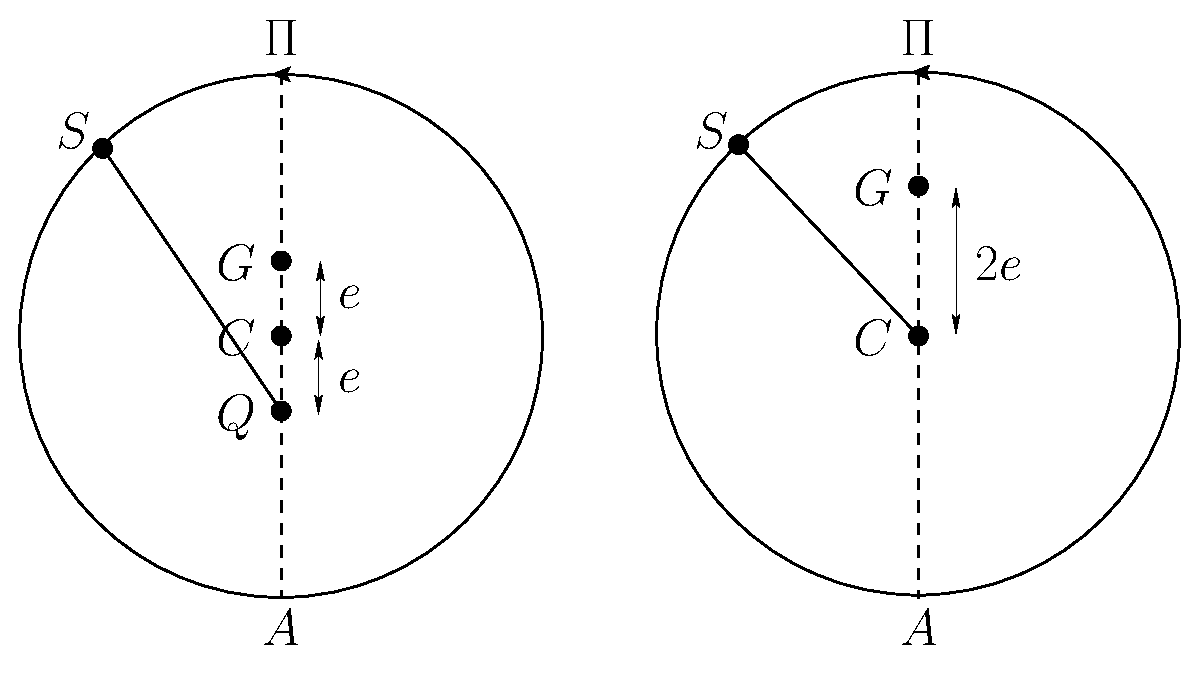
\includegraphics[height=3in]{epsfiles/sun.eps}}
\caption{Hipparchus' (and Ptolemy's) model of the Sun's apparent orbit  about the Earth (right) compared to the optimal  model (left).  The
radius vectors in both models rotate uniformly. Here, $S$ is the Sun, $G$ the Earth, $C$ the geometric center of the orbit, $Q$ the equant, $\Pi$ the perigee, and $A$ the apogee. The radius of the orbit is normalized to unity.}\label{fsun}   
\end{figure}

The geocentric model of the Solar System outlined previously represents a perfected version
of Ptolemy's model, constructed with 
a knowledge of the true motions of the planets around the Sun.
Not surprisingly, the  model actually described in the Almagest deviates
somewhat from this ideal form. In the following, we shall
refer to these deviations as ``errors'', but this should not be understood
in a pejorative sense.

Ptolemy's first error lies in his model of the Sun's apparent motion around the Earth, which he inherited
from Hipparchus. Figure~\ref{fsun} compares what Ptolemy actually
did, in this respect, compared to
what he should have done in order to be completely consistent
with the rest of his model. Let us normalize the mean radius of the Sun's
apparent orbit  to unity, for the sake of clarity.
 Ptolemy should
have adopted the model shown on the left in Figure~\ref{fsun}, in which the Earth
is displaced from the center of the Sun's orbit a distance $e=0.0167$ (the eccentricity of the Earth's orbit around the Sun) towards the perigee (the point of the Sun's closest approach
to the Earth), and the equant is displaced the same distance in the opposite
direction. The instantaneous angular position of the Sun is then obtained
by allowing the radius vector connecting the equant to the Sun to rotate uniformly at the Sun's mean orbital angular velocity. Of course, this implies that the
Sun rotates non-uniformly about the Earth. Ptolemy actually adopted the Hipparchian model
shown on the right in Figure~\ref{fsun}. In this model, the Earth is displaced
a distance $2e$ from  the center of the Sun's orbit in the direction of the perigee,
and the Sun rotates at a uniform rate (that is, the radius vector $CS$ rotates uniformly). It turns out that, to first order in $e$, these two
models are equivalent in terms of their ability to predict the angular position of the Sun relative to the Earth. (See Chapter~\ref{ckep}.) Nevertheless, the Hipparchian
model is incorrect, because it predicts too large (by a factor of two) a variation in  the radial distance of the Sun from the Earth (and, hence,  the angular size of the Sun)  during the
course of a year. (See Chapter~\ref{ckep}.) Ptolemy probably adopted
the Hipparchian model because his Aristotelian leanings prejudiced him in favor of uniform circular motion whenever this was consistent with observations.
(It should be noted that Ptolemy was not  interested in explaining the relatively small variations in the angular size of the Sun during the year; presumably, because this effect would have been very difficult for him to accurately measure.)

Ptolemy's next error was to neglect the non-uniform rotation of the
superior planets on their epicycles. This is equivalent to neglecting
the orbital eccentricity of the Earth (recall that the epicycles of the superior
planets actually represent the Earth's orbit) compared to those of
the superior planets. It turns out that this is a fairly good approximation,
because the superior planets all have significantly greater orbital eccentricities
than the Earth. Nevertheless, 
neglecting  the non-uniform rotation of the
superior planets on their epicycles has the unfortunate effect of obscuring the tight coupling between
the apparent motions of these planets, and that of the Sun. The radius vectors connecting the epicycle centers of the
superior planets to the planets themselves should always all point  exactly in the
same direction as that of the Sun relative to the Earth.
When the aforementioned non-uniform rotation is neglected, the radius
vectors instead point in the direction of the  mean Sun  relative to
the Earth. The {\em mean Sun}\/ is a fictitious body that has the
same apparent orbit around the Earth as the real Sun, but that circles
the Earth at a uniform rate. The mean Sun only coincides with the
real Sun twice a year.

Ptolemy's third error is associated with his treatment of the
inferior planets. As we have seen, in going from the superior to the
inferior planets, deferents and epicycles effectively swap roles. 
For instance, it is the deferents  of the inferior planets, rather than the epicycles, that represent
the Earth's orbit. Hence, for the sake of consistency with his treatment of
the superior planets, Ptolemy should have neglected the non-uniform
rotation of the epicycle centers around the deferents of the inferior
planets, and retained the non-uniform rotation of the planets themselves around the
epicycle centers. Instead, he did exactly the opposite. This
is equivalent to neglecting the inferior planets' orbital eccentricities relative to
that of the Earth. It follows that this approximation only works when an inferior
planet has a significantly smaller  orbital eccentricity than that of the Earth.
It turns out that this is indeed the case for Venus, which has the smallest eccentricity
of any planet in the Solar System. Thus, Ptolemy was able to
successfully account for the apparent motion of Venus. Mercury, on the
other hand, has a much larger orbital eccentricity than the Earth. Moreover, it
is particularly difficult to obtain good naked-eye positional data for Mercury, because this planet always appears 
very close to the Sun in the sky. Consequently,
Ptolemy's Mercury data was highly inaccurate.
 Not surprisingly, Ptolemy was not able to account for the apparent motion of Mercury
using his standard deferent-epicycle approach. Instead, in order to fit the data, he was forced
to introduce an additional, and entirely spurious, epicycle into his  model of
Mercury's orbit.

Ptolemy's fourth, and possibly largest, error is associated with his treatment
of the Moon. It should be noted that the Moon's motion around the
Earth is extremely complicated in nature, because it is strongly perturbed by the Sun,  and was not fully understood until
the early 20th century AD. Ptolemy constructed an ingenious geometric
model of the Moon's orbit that was capable of predicting
the lunar ecliptic longitude to reasonable accuracy. Unfortunately, this
model necessitates a monthly variation in the Earth-Moon distance  by a factor of about two, 
which  implies a similarly large variation in the Moon's angular diameter. However, the observed variation in the   Moon's diameter is very much smaller than this. Hence, Ptolemy's model of lunar motion is not even approximately correct.

Ptolemy's fifth error is associated with his treatment of planetary
ecliptic latitudes. Given that the deferents and epicycles of
the superior planets represent the orbits of the planets themselves around the
Sun, and the Sun's apparent orbit around the Earth, respectively, it follows
that one should take the slight inclination of planetary orbits to
the ecliptic plane (that is, the plane of the Sun's apparent orbit)
into account by tilting the deferents of superior planets, while keeping their epicycles
parallel to the ecliptic. Similarly, given that the epicycles and deferents of
inferior planets represent the orbits of the planets themselves around the
Sun, and the Sun's apparent orbit around the Earth, respectively, one should tilt the epicycles of
inferior planets, while keeping their deferents parallel to the ecliptic. 
Finally, because the inclination of  planetary orbits are all essentially constant in time, the inclinations
of the epicycles and deferents should also be constant. 
Unfortunately, when Ptolemy constructed his theory of
planetary latitudes, he tilted  the both deferents and epicycles of
all of the planets. Even worse, he allowed the inclinations of the epicycles to
the ecliptic plane to vary in time. The net result is a theory which is far more
complicated than is necessary.

The final failing in Ptolemy's model of the Solar System lies in its  scale invariance. 
Using angular position data alone, Ptolemy was  able to determine the ratio 
of the epicycle radius to that of the deferent for each planet, but was
not able to determine the  relative sizes  of the deferents of different planets. 
In order to break this scale invariance it is necessary to make an
additional assumption; namely, that the Earth orbits the Sun. This
brings us to Copernicus.

\section{Copernicus's Model of the Solar System}
The Polish astronomer Nicolaus Copernicus (1473--1543 AD) studied the
Almagest assiduously, but eventually became dissatisfied with
Ptolomy's approach. The main reason for this dissatisfaction was
not the geocentric nature of Ptolomy's model, but rather the fact that it
mandates that heavenly bodies  execute non-uniform circular
motion. Copernicus, like Aristotle, was convinced that the supposed perfection
of the heavens requires  such bodies to execute uniform  circular motion only. Copernicus was thus spurred to construct his own
model of the Solar System, which was described in his book {\em De Revolutionibus Orbium Coelestium}\/ (On the Revolutions of the Heavenly Spheres), published in the year of his death.

The most well-known aspect of Copernicus's model is the fact that it
is  heliocentric. As has already been mentioned, when describing
the motion of the Sun, Moon, and planets relative to the Earth, it makes
little practical difference whether one adopts a geocentric or a heliocentric
model of the Solar System. Having said this, the heliocentric approach does have one large advantage. If we accept that the Sun,  and not the Earth,
is stationary, then it immediately follows that the epicycles of the
superior planets, and the deferents of the inferior planets,  represent the Earth's orbit around the Sun. Hence, all of these circles
must be the same size. This realization allows us to break the
scale invariance which is one of the main failings of Ptolemy's
model. Thus, the ratio of the deferent radius to that of the
epicycle for a superior planet, which is easily inferred from observations,
actually corresponds to the ratio of planet's orbital radius to that of the
Earth. Likewise, the ratio of the epicycle radius to that of the deferent
for an inferior planet, which is again easily determined observationally, also corresponds to the ratio of the planet's
orbital radius to that of the Earth. Using this type of reasoning,
Copernicus was able to construct the first accurate scale model
of the Solar System, and to firmly establish the order in which the planets
orbit the Sun. In some sense, this was his main achievement.

Copernicus's insistence that heavenly bodies should only move in uniform 
circles lead him to reject Ptolemy's  equant scheme, and to  replace
it with the scheme illustrated in Figure~\ref{fplan}. According to Copernicus, a heliocentric
planetary orbit is a combination of  two  circular motions. The first is 
the motion of the planet around a small circular epicycle, and the second is the motion of the center of
the epicycle around the Sun on  a circular deferent. Both motions are  uniform, and in the same direction.
However, the former motion is twice as fast as the latter. In addition, the Sun is displaced
from the center of the deferent in the direction of the perihelion, the displacement being
proportional to the orbital eccentricity. Furthermore, the Sun's displacement
is  three  times greater than the radius of the epicycle. Finally, the
radius of the deferent is equal to the major radius of the planetary orbit. It turns
out that Copernicus' scheme is a marginally less accurate approximation  than Ptolemy's to 
a low eccentricity Keplerian orbit. (See Chapter~\ref{ckep}.) 

Copernicus modeled the
orbit of the Earth around the Sun using an Hipparchian scheme (see Figure~\ref{fsun}) in which the Earth moves
uniformly around an eccentric circle.  Unfortunately, such a scheme exaggerates the variation in the
radial distance between the Earth and the Sun during the course of a year by a factor of two, and so
introduces significant errors into the calculation of the parallax of the planets due to the motion of the Earth. 
On the other hand, Copernicus' model of the Moon's orbit around the Earth is a considerable improvement on Ptolemy's, because
it does not grossly exaggerate the monthly variation in the Earth-Moon distance. 
Like Ptolemy, Copernicus  introduced an additional spurious epicycle into his model
of Mercury's orbit, and erroneously allowed the
inclination of his planetary orbits to vary slightly  in time. 

In summary, Copernicus's model of the Solar System contains approximately the 
 same number of epicycles as Ptolemy's, the only difference being that Copernicus' epicycles are much 
 smaller than Ptolemy's.  Indeed, the model of Copernicus is about as complicated, and not appreciably more accurate, than that described in the  Almagest. 
In this respect, Copernicus cannot be said to have demonstrated
the correctness of his heliocentric approach on the basis of observational data. 

\begin{figure}
\centerline{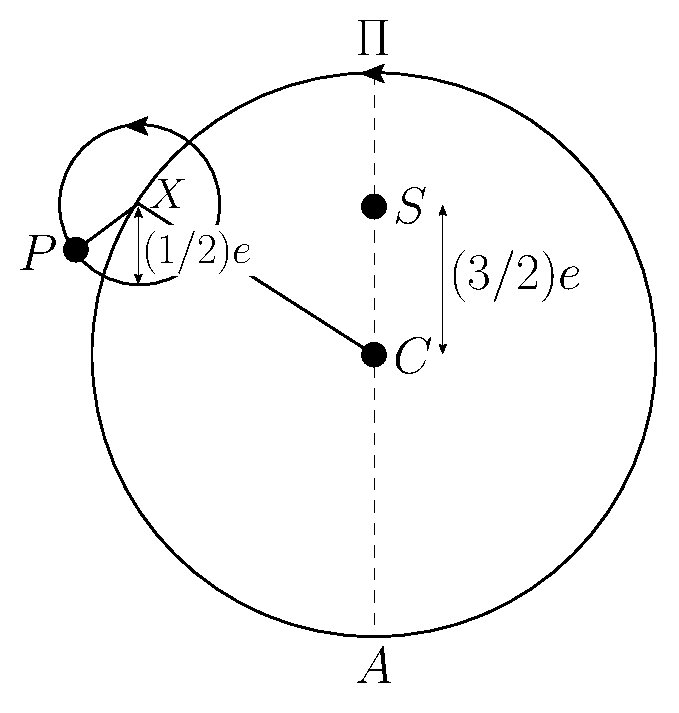
\includegraphics[height=3in]{epsfiles/fig1.2x.eps}}
\caption{Copernicus' model of a heliocentric planetary orbit. Here, $S$ is the Sun, $P$ the planet, $C$ the geometric center of the deferent, $X$ the center of the epicycle, $\Pi$ the perihelion, and $A$ the aphelion. The radius vectors $CX$ and $XP$ both rotate uniformly in the
same direction,
but $XP$ rotates twice as fast as $CX$. The major radius of the orbit is normalized to unity.}\label{fplan}   
\end{figure}

\section{Kepler's Model of the Solar System}
Johannes Kepler (1571--1630 AD) was fortunate  to inherit an extensive set of naked-eye solar, lunar, and planetary angular position data
 from the Danish astronomer Tycho Brahe (1546--1601 AD). This data
 extended over many decades, and was of unprecedented accuracy.
 
 Although Kepler adopted the heliocentric approach of Copernicus,
 what he effectively first did was to  perfect Ptolemy's model of the Solar System (or, rather,
 its heliocentric equivalent). Thus, Kepler replaced Ptolemy's
 erroneous equantless model of the Sun's apparent orbit around the
 Earth with a corrected version containing an equant; in the process,
 halving the eccentricity of the orbit. (See Figure~\ref{fsun}.)  Kepler also introduced equants
 into the epicycles of the superior and inferior planets. Once he had perfected Ptolemy's model, the heliocentric nature of
 the Solar System became manifestly apparent to Kepler. For instance,
 he found that the epicycles of the superior planets, the Sun's
 apparent orbit around the Earth, and the deferents of the inferior
 planets, all had exactly the  same eccentricity. The obvious implication
  is that these circles all correspond to some common motion within the
 Solar System; in fact, the motion of the Earth around the Sun.
 
 Once Kepler had corrected the Almagest model, he compared its predictions
 with his observational data. In particular, Kepler investigated 
 the apparent motion of Mars in the night sky. Kepler found that his  model performed extremely well,
 but that there remained small differences between its predictions and the observational data. The maximum discrepancy was about $8'$; that is, about one
 quarter of the apparent size of the
 Sun. By the standards of naked-eye astronomy, this was a very small discrepancy. Nevertheless, given the incredible accuracy of Tycho Brahe's
 observations, the discrepancy was still significant. Thus, Kepler embarked on an epic new series
 of calculations which eventually lead him to the conclusion that the
 planetary orbits are actually eccentric ellipses, rather than eccentric circles. 
 Kepler published the results of his research in  his treatise {\em Astronomia Nova}\/ (New Astronomy) in 1609 AD.
 It is
 interesting to note that had Tycho's data been a little less accurate,
 or had the orbit of Mars been a little less eccentric, Kepler might well 
 have settled for a model which was kinematically equivalent to
 a perfected version of the model described in the Almagest. We can also
 appreciate that, given the far less accurate observational data available to
 Ptolemy, there was no way in which he could have discerned the
 very small difference between elliptical planetary orbits and the eccentric
 circular orbits employed in the Almagest.
 
 \section{Purpose of Treatise}
As we have seen, misconceptions abound regarding the details of Ptolemy's model of the Solar System, as well as  its scientific merit. Part of the reason for this is 
that the Almagest is an extremely difficult book for a
modern reader to comprehend.  For instance, virtually all of its theoretical results are justified via lengthy  and opaque geometric
proofs. Moreover, the  plane and
spherical trigonometry employed by Ptolemy is of a rather primitive  nature, and,
consequently, somewhat unwieldy. Dates are also a major stumbling block, because three different systems are used in the Almagest,
all of which are archaic, and essentially meaningless to the modern reader.
Another difficulty is the unfamiliar, and far from optimal, ancient Greek method of representing numbers and fractions.
Finally, the terminology employed in the Almagest is, in many instances, significantly different to that used in modern
astronomy textbooks.

The aim of this treatise is to reconstruct Ptolemy's model of the Solar System employing
modern  mathematical methods, standard dates, and conventional astronomical terminology. It
is hoped that the resulting model will enable the reader to comprehend the full extent of Ptolemy's scientific
achievement. In fact, the model described
in this work is a somewhat improved version of Ptolemy's, in that
all of the  previously mentioned deficiencies   have been corrected. Furthermore, Ptolemy's equant scheme has been replaced by a Keplerian scheme, expanded to second order in the planetary
eccentricities.
It should be noted, however, that these two schemes are essentially indistinguishable for
small eccentricity orbits. 
Certain aspects of the Almagest have not been reproduced. For instance, it was not thought necessary to instruct the reader on how to construct
trigonometric tables, or primitive astronomical instruments. Furthermore, no attempted has been made to derive any of the model parameters directly from
 observational data, because the orbital elements and physical properties of the Sun, Moon, and planets are, by now, extremely well established. Any detailed discussion of the fixed stars has also been omitted, because stellar positions  are also very well established, and the apparent motion
 of the stars in the sky is comparatively straightforward compared to those of the Sun, the Moon, and the planets. 
 What remains is a mathematical model of the Solar
 System that is surprisingly accurate (the maximum errors in the ecliptic
 longitudes of the Sun, Moon, Mercury, Venus, Mars, Jupiter, and
 Saturn during the years 1995--2006 AD are $0.7'$, $14'$, $28'$, $10'$,
 $14'$, $4'$, and $1'$, respectively), yet sufficiently simple that all of the
 necessary calculations can be performed by hand, with the aid of tables. The form of the calculations, as well as the layout of the tables,
 is, for the most part, fairly similar to those found in the Almagest. Many examples
 of the use of the tables are provided. 

\chapter{Spherical Astronomy}
\section{Celestial Sphere}
It is often helpful to imagine that celestial objects are attached to a vast sphere centered on the
earth. This fictitious construction is known as the {\em celestial sphere}. The earth's dimensions are assumed 
to be infinitesimally small compared to those  of the sphere (since the distance of a typical celestial object from 
the earth is very much larger than the earth's radius).  It follows that only {\em half}\/ of the sphere  is visible from
any particular observation site on the earth's surface. Furthermore, the angular position of a given celestial object (relative to some fixed celestial reference) is the 
same at all such sites. In other words, there is negligible {\em parallax}\/ associated
with viewing the same celestial object from different observation sites on the surface of the earth.\footnote{
 The one exception to this rule is the moon, which is sufficiently close to the earth
 that its parallax is significant---see Sect.~\ref{spara}.}

\section{Celestial Motions}
Celestial objects exhibit {\em two}\/ different types of motion. The first motion is such that the whole celestial sphere, and all of the
celestial objects attached to it, rotates
uniformly from east to west once every 24 (sidereal) hours, about a fixed axis passing through the earth's north and south poles. This type of motion is called {\em diurnal motion}, and is a consequence of the earth's daily  rotation. Diurnal motion preserves the relative angular positions of all celestial objects. However, certain
celestial objects, such as the sun, the moon, and the planets, possess a second motion, superimposed on the
first, which causes their angular positions to slowly change relative to one another, and to the fixed stars. This {\em intrinsic
motion}\/ of objects in the solar system is due to a combination of the earth's orbital motion about the sun, and the orbital motions of the moon and the planets about the earth and the sun, respectively.

\section{Celestial Coordinates}
Consider Fig.~\ref{f1}. The celestial sphere rotates about the {\em celestial axis}, $PP'$,  which is the imagined  extension of the  earth's axis of rotation. This axis intersects the celestial sphere at the {\em north celestial pole}, $P$, and the {\em south celestial pole}, $P'$. It follows that the two celestial poles are
unaffected by diurnal motion, and remain fixed in the sky.

\begin{figure}
\epsfysize=3in
\centerline{\epsffile{epsfiles/sphere1.eps}}
\caption[\em The celestial sphere.]{\em The celestial sphere. $G$, $P$, $P'$, $V$, and $V'$ represent the earth, north celestial
pole, south celestial pole, vernal equinox, and  autumnal equinox, respectively. $VUV'U'$ is the celestial equator, and $PP'$ the
celestial axis.}\label{f1}
\end{figure}

The {\em celestial equator}, $VUV'U'$, is the intersection of the earth's equatorial plane with the celestial
sphere, and is therefore
perpendicular to the celestial axis. The so-called {\em vernal equinox}, $V$, is a particular point on the
celestial equator that is used as the origin of celestial longitude. Furthermore, the {\em autumnal equinox}, $V'$,
is a point which lies directly opposite the vernal equinox on the celestial equator. Let the line $UU'$ lie in the plane of the celestial equator
such that it is perpendicular to $VV'$, as shown in the figure.

It is helpful to define  three, right-handed, mutually perpendicular, unit vectors: ${\bf v}$, 
${\bf u}$, and ${\bf p}$.
Here, ${\bf v}$ is directed from the earth to the vernal
equinox, ${\bf u}$ from the earth to point $U$, and ${\bf p}$ from the
earth to the north celestial pole---see Fig.~\ref{f1}.

\begin{figure}
\epsfysize=3in
\centerline{\epsffile{epsfiles/sphere2.eps}}
\caption[\em Celestial coordinates.]{\em Celestial coordinates. $R$ is a celestial object, and $R'$ its
projection onto the plane of the celestial equator, $VR'V'$.}\label{f2}
\end{figure}

Consider a general celestial object, $R$---see Fig.~\ref{f2}. The location of $R$ on the celestial sphere
is conveniently specified by  two angular coordinates, $\delta$ and $\alpha$. Let $GR'$ be the
projection of $GR$ onto the equatorial plane. The coordinate $\delta$, which is known as {\em declination}, is  the angle subtended between $GR'$ and $GR$. Objects north of the celestial equator have positive
declinations, and {\em vice versa}. It follows that objects on the celestial equator have declinations of $0^\circ$,
whereas the north and south celestial poles have declinations of $+90^\circ$ and $-90^\circ$, respectively.
The coordinate $\alpha$, which is known as {\em right ascension}, is the angle subtended between 
$GV$ and $GR'$. Right ascension increases from west to east ({\em i.e.}, in the opposite direction to the
celestial sphere's diurnal rotation). Thus, the vernal and autumnal equinoxes have right ascensions of $0^\circ$ and $180^\circ$, respectively. Note that $\alpha$ lies in the range $0^\circ$ to
$360^\circ$. Right ascension is sometimes measured in hours, instead of degrees, with one hour corresponding to
$15^\circ$ (since it takes 24 hours for the celestial sphere to complete
one diurnal rotation). In this scheme, the vernal and autumnal equinoxes
have right ascensions of $0$ hrs.\ and $12$ hrs., respectively. Moreover, $\alpha$ lies in the
range $0$  to 24 hrs. (Incidentally, in this treatise, $\alpha$ is measured
relative to the mean equinox at date, unless otherwise specified.)
Finally, let ${\bf r}$ be a unit vector which is directed from the earth to $R$---see Fig.~\ref{f2}. It is easily
demonstrated that 
\begin{equation}\label{e1}
{\bf r} = \cos\delta\,\cos\alpha\,{\bf v} + 
\cos\delta\,\sin\alpha\,{\bf u} + \sin\delta\,{\bf p},
\end{equation}
and
\begin{eqnarray}\label{e2}
\sin\delta &=& {\bf r}\cdot {\bf p},\\[0.5ex]
\tan\alpha &=& \left(\frac{{\bf r}\cdot{\bf u}}{{\bf r}\cdot {\bf v}}\right).\label{e3}
\end{eqnarray}

\section{Ecliptic Circle}
During the course of a year, the sun's intrinsic motion causes it to trace out a fixed circle which bisects the celestial sphere. This circle is known as the {\em ecliptic}. The sun travels around the ecliptic from west to east ({\em i.e.}, in the opposite direction
to the celestial sphere's diurnal rotation). Moreover, the ecliptic circle is inclined at a fixed angle of $\epsilon = 23^\circ 26'$ to the celestial equator.
This angle actually represents the fixed inclination of the earth's axis of rotation to the normal to its orbital
plane.\footnote{In fact, $\epsilon$ is very slowly decreasing in time. The value of
$\epsilon$ used in  the Almagest is $23^\circ 51'$. However, the true value of $\epsilon$  in Ptolemy's day was $23^\circ 41'$.}

\begin{figure}
\epsfysize=3in
\centerline{\epsffile{epsfiles/sphere3.eps}}
\caption[\em The ecliptic circle.]{\em The ecliptic circle. $P$, $P'$, $Q$, $Q'$, $V$, $V'$, $S$, 
and $S'$ denote the north celestial pole, south celestial pole, north ecliptic pole, south
ecliptic pole, vernal equinox, autumnal equinox, summer solstice, and winter
solstice, respectively. $VUV'U'$ is the celestial equator, $VSV'S'$ the ecliptic, and $PP'$ the
celestial axis.}\label{f3}
\end{figure}

The vernal equinox, $V$, is defined as the point at which the ecliptic crosses the celestial equator
from south to north (in the direction of the sun's ecliptic motion)---see Fig.~\ref{f3}. Likewise, the autumnal equinox, $V'$, is the point at which the ecliptic crosses the
celestial equator from north to south.  In addition, the {\em summer solstice}, $S$, is the
point on the ecliptic which is furthest north of the celestial equator, whereas the
{\em winter solstice}, $S'$, is the  point which is furthest south. It follows that the lines $VV'$ and $SS'$
are perpendicular. Let $QQ'$ be the normal to the plane of the ecliptic which passes through the earth, as shown in Fig.~\ref{f3}.  
Here, $Q$ is termed the {\em northern ecliptic pole}, and $Q'$ the {\em southern ecliptic pole}. 
It is easily demonstrated that
\begin{eqnarray}
{\bf s} &=& \cos\epsilon\,{\bf u}+ \sin\epsilon\,{\bf p},\label{e4}\\[0.5ex]
{\bf q} &=& -\sin \epsilon\,{\bf u} + \cos\epsilon\,{\bf p},\label{e5}
\end{eqnarray}
where ${\bf s}$ is a unit vector which is directed from the earth to the summer solstice, and ${\bf q}$ a unit vector which is directed from the earth to the north ecliptic pole---see Fig.~\ref{f3}. We can also write
\begin{eqnarray}
{\bf u} &=& \cos\epsilon\,{\bf s} - \sin\epsilon\,{\bf q},\label{e4p}\\[0.5ex]
{\bf p} &=& \sin\epsilon\,{\bf s} + \cos\epsilon\,{\bf q}.\label{e5p}
\end{eqnarray}
Thus, ${\bf v}$, ${\bf s}$, and ${\bf q}$ constitute another right-handed, mutually perpendicular, set of unit vectors. 

\begin{figure}
\epsfysize=3in
\centerline{\epsffile{epsfiles/sphere4.eps}}
\caption[\em Ecliptic coordinates.]{\em Ecliptic coordinates. $G$ is the earth, $R$ a celestial
object, and $R'$ its projection onto the ecliptic plane, $VR'V'$.}\label{f4}
\end{figure}

\section{Ecliptic Coordinates}
It is convenient to specify the positions of the sun, moon, and planets in the sky using
a pair of angular coordinates, $\beta$ and $\lambda$, which are measured with respect to the
ecliptic, rather than the celestial equator. Let $R$ denote a celestial object, and $GR'$ the
projection of the line $GR$ onto the plane of the ecliptic, $VR'V'$---see Fig.~\ref{f4}. The coordinate $\beta$, which
is known as {\em ecliptic latitude}, is the angle subtended between $GR'$ and $GR$. Objects north
of the ecliptic plane have positive ecliptic latitudes, and {\em vice versa}. The coordinate $\lambda$,
which is known as {\em ecliptic longitude}, is the angle subtended between $GV$ and
$GR'$. Ecliptic longitude increases from west to east ({\em i.e.}, in the same direction that the sun travels
around the ecliptic). (Again, in this treatise, $\lambda$ is measured relative
to the mean equinox at date, unless specified otherwise.)
Note that the basis vectors in the ecliptic coordinate system are
${\bf v}$, ${\bf s}$, and ${\bf q}$, whereas the corresponding basis vectors in the
celestial coordinate system are
${\bf v}$, ${\bf u}$, and ${\bf p}$---see Figs.~\ref{f1} and \ref{f3}. By analogy with Eqs.~(\ref{e1})--(\ref{e3}), we can write
\begin{eqnarray}\label{e8w}
{\bf r} &=& \cos\beta\,\cos\lambda\,{\bf v} + \cos\beta\,\sin\lambda\,{\bf s} +\sin\beta\,{\bf q},\label{e1p}\\[0.5ex]
\sin\beta &=& {\bf r}\cdot {\bf q},\\[0.5ex]
\tan\lambda &=& \left(\frac{{\bf r}\cdot{\bf s}}{{\bf r}\cdot {\bf v}}\right),
\end{eqnarray}
where ${\bf r}$ is a unit vector which is directed from $G$ to $R$. 
Hence, it follows from Eqs.~(\ref{e1}), (\ref{e4}), and (\ref{e5}) that
\begin{eqnarray}
\sin\beta &=& \cos\epsilon\,\sin\delta - \sin\epsilon\,\cos\delta\,\sin\alpha,\\[0.5ex]
\tan\lambda &=& \frac{\cos\epsilon\,\cos\delta\,\sin\alpha+\sin\epsilon\,\sin\delta}{\cos\delta\,\cos\alpha}.
\end{eqnarray}
These expressions specify the transformation from celestial to ecliptic
coordinates. The inverse transformation follows from Eqs.~(\ref{e2}), (\ref{e3}), and (\ref{e4p})--(\ref{e1p}):
\begin{eqnarray}\label{e10}
\sin\delta &=& \cos\epsilon\,\sin\beta +\sin\epsilon\,\cos\beta\,\sin\lambda,\\[0.5ex]
\tan\alpha&=&  \frac{\cos\epsilon\,\cos\beta\,\sin\lambda-\sin\epsilon\,\sin\beta }{\cos\beta\,\cos\lambda}.\label{e11}
\end{eqnarray}

Figures~\ref{map1} and \ref{map2} show all stars of visible magnitude less than $+6$ lying
within $15^\circ$ of the ecliptic. Table~\ref{tstar} gives the ecliptic longitudes, ecliptic latitudes, and
visible magnitudes of a selection
of these stars which lie within $10^\circ$ of the ecliptic. The figures and table can
be used 
 to convert ecliptic longitude and latitude into approximate position
in the sky against the backdrop of the fixed stars.

\section{Signs of the Zodiac}\label{szod}
The {\em signs of the zodiac}  are a well-known set of names given
to $30^\circ$ long segments of the ecliptic circle. Thus, the sign of Aries extends
over the range of ecliptic longitudes $0^\circ$--$30^\circ$, the sign of Taurus
over the range $30^\circ$--$60^\circ$, and so on. Note that, as
a consequence of the precession of the equinoxes, the signs
of the zodiac no longer coincide with the constellations of the same name
(see Figs.~\ref{map1} and \ref{map2}).
The 12 zodiacal signs are listed in the table below.  It can be seen from the table that ecliptic longitude $72^\circ$ corresponds to the
twelfth degree of Gemini, and ecliptic longitude $242^\circ$  to the second degree of
Sagittarius, {\em etc.}
\begin{table}[h]
\centering
\begin{tabular}{lcl|lcl|lcl}
Sign & Abbr.\ & Longitude & Sign & Abbr.\ &Longitude & Sign & Abbr.\ &  Longitude\\[-0.0ex]\hline
&&&&&&&&\\[-1.8ex]
Aries & AR & $~~0^\circ$--$30^\circ$ & Leo & LE & $120^\circ$--$150^\circ$&Sagittarius & SG & $240^\circ$--$270^\circ$\\
Taurus & TA & $30^\circ$--$60^\circ$ & Virgo & VI & $150^\circ$--$180^\circ$ & Capricorn & CP & $270^\circ$--$300^\circ$\\
Gemini & GE & $60^\circ$--$90^\circ$ & Libra & LI & $180^\circ$--$210^\circ$ & Aquarius & AQ & $300^\circ$--$330^\circ$\\
Cancer & CN & $90^\circ$--$120^\circ$ & Scorpio & SC & $210^\circ$--$240^\circ$ & Pisces & PI & $330^\circ$--$360^\circ$\\
\end{tabular}
\end{table}

\section{Ecliptic Declinations and Right Ascenesions.}
According to Eqs.~(\ref{e10}) and (\ref{e11}), the celestial coordinates of a point on the ecliptic circle ({\em i.e.}, $\beta = 0$) which has ecliptic
longitude $\lambda$ are specified by
\begin{eqnarray}\label{e15q}
\sin\,\delta &=& \sin\epsilon\,\sin\lambda,\\[0.5ex]
\tan\,\alpha&=&  \cos\epsilon\,\tan\lambda.\label{e15r}
\end{eqnarray}
The above formulae have been used to construct
Tables~\ref{tec1} and \ref{tec2}, which  list the declinations and right ascensions of a set of equally spaced points on the ecliptic circle.

\section{Local Horizon and Meridian}
Consider a general observation site $X$ on the surface of the earth. (Note that, in the following, it is
tacitly assumed that the site lies the earth's northern hemisphere. However, the analysis also
applies to sites situated in the the southern hemisphere.)
The local {\em zenith}\/ $Z$ is the point on the celestial sphere which is directly overhead at $X$,
whereas the {\em nadir}\/ $Z'$ is the point which is directly underfoot---see Fig.~\ref{f5}. The {\em horizon}\/
is the tangent plane to the earth at $X$, and divides the celestial sphere into two halves. The upper half,
containing the zenith, is visible from site $X$, whereas the lower half is invisible. 

\begin{figure}
\epsfysize=3in
\centerline{\epsffile{epsfiles/sphere5.eps}}
\caption[{\em A general observation site on the earth's surface.}]{\em A general observation site $X$, of latitude $L$,  on the surface of the earth. $P$, $P'$, $Z$, and $Z'$
denote the directions to the north celestial pole, south celestial pole, zenith, and nadir, respectively. The line
$NS$ represents the local horizon.}\label{f5}
\end{figure}

\begin{figure}
\epsfysize=3in
\centerline{\epsffile{epsfiles/sphere6.eps}}
\caption[{\em The local horizon and meridian.}]{\em The local horizon and meridian. $N$, $S$, $E$, $W$
denote the north. south, east, and west compass points, $Z$ the
zenith, and $P$ the north celestial pole. $NESW$ is the horizon, and
$NPZS$ the meridian.}\label{f6}
\end{figure}

Figure~\ref{f6} shows the visible half of the celestial sphere at observation site $X$. 
Here, $NESW$ is the local horizon, and  $N$, $E$, $S$, and $W$ are
the north, east, south, and west compass points, respectively. The plane $NPZS$,
which passes through the north and south compass points, as well as the zenith,
is known as the local {\em meridian}. The meridian is perpendicular
to the horizon. The north celestial pole lies in the meridian plane, and
is elevated an angular distance $L$ above the north compass point---see Figs.~\ref{f5} and \ref{f6}. Here,
$L$ is the terrestrial {\em latitude}\/ of observation site $X$. It is helpful to
define three, right-handed, mutually perpendicular,  local unit vectors: ${\bf e}$, ${\bf n}$, and ${\bf z}$.
Here, 
${\bf e}$ is directed toward the east compass point, ${\bf n}$ toward the north compass point, and ${\bf z}$  toward the zenith---see Fig.~\ref{f6}. 

\begin{figure}
\epsfysize=3in
\centerline{\epsffile{epsfiles/sphere8.eps}}
\caption[{\em The local meridian.}]{\em The local meridian.}\label{f7}
\end{figure}

Figure~\ref{f7} shows the meridian plane at $X$. Let the line $MM'$ lie
in this plane such that it is perpendicular to the celestial axis, $PP'$. Moreover, let
$M$ lie in the visible hemisphere. It is helpful to define the unit vector ${\bf m}$ which
is directed toward $M$, as shown in the diagram. It is easily seen that
\begin{eqnarray}\label{e14}
{\bf n} &=& \cos L\,{\bf p} - \sin L\,{\bf m},\\[0.5ex]
{\bf z} &=& \sin L\,{\bf p} + \cos L\,{\bf m}.\label{e15}
\end{eqnarray}

\begin{figure}
\epsfysize=3in
\centerline{\epsffile{epsfiles/sphere9.eps}}
\caption[{\em The local celestial equator.}]{\em The local celestial equator.}\label{f8}
\end{figure}

Figure~\ref{f8} shows the celestial equator viewed from observation site $X$. Here, $\alpha_0$ is
the right ascension of the celestial objects culminating ({\em i.e.}, reaching
their highest altitude in the sky) on the meridian at the time of observation. Incidentally, it is
easily demonstrated that all objects culminating on the meridian at
any instant in time have the {\em same}\/ right ascension. Note that the angle $\alpha_0$
increases uniformly in time, at the rate of $15^\circ$ a (sidereal) hour, due to the diurnal motion of the celestial
sphere. It can be seen from the diagram that
\begin{eqnarray}
{\bf m} &=& \sin \alpha_0\,{\bf u} + \cos \alpha_0\,{\bf v},\\[0.5ex]
{\bf e} &=&\cos \alpha_0 \,{\bf u} -\sin \alpha_0\,{\bf v}.\label{e17}
\end{eqnarray}
Thus, from Eqs.~(\ref{e14}) and (\ref{e15}),
\begin{eqnarray}
{\bf e} &=& -\sin \alpha_0\,{\bf v} + \cos \alpha_0\,{\bf u},\\[0.5ex]
{\bf n} &=& -\sin L\,\cos \alpha_0\,{\bf v} - \sin L\,\sin \alpha_0\,{\bf u} + \cos L\,{\bf p},\label{xx}\\[0.5ex]
{\bf z} &=& \cos L\,\cos \alpha_0\,{\bf v} + \cos L\,\sin \alpha_0\,{\bf u} + \sin L\,{\bf p}.\label{zz}
\end{eqnarray}
Similarly, from Eqs.~(\ref{e4p}) and (\ref{e5p}),
\begin{eqnarray}
{\bf e}&=& -\sin \alpha_0\,{\bf v} + \cos\epsilon\,\cos \alpha_0\,{\bf s} - \sin\epsilon\,\cos \alpha_0\,{\bf q},\label{e25w}\\[0.5ex]
{\bf n} &=& -\sin L\,\cos \alpha_0\,{\bf v} + (\cos L\,\sin \epsilon-\sin L\,\cos \epsilon\,\sin \alpha_0)\,{\bf s} + (\cos L\,\cos \epsilon\nonumber\\[0.5ex] &&+\sin L\,\sin \epsilon\,\sin \alpha_0)\,{\bf q},\label{e24w}\\[0.5ex]
{\bf z} &=& \cos L\,\cos \alpha_0\,{\bf v} + (\sin L\,\sin\epsilon + \cos L\,\cos\epsilon\,\sin \alpha_0)\,{\bf s} + (\sin L\,\cos\epsilon\nonumber\\[0.5ex]&&-\cos L\,\sin\epsilon\,\sin \alpha_0)\,{\bf q}.\label{e26w}
\end{eqnarray}

\section{Horizontal Coordinates}
It is convenient to specify the positions of celestial objects  in the sky, when viewed from
a particular observation site, $X$, on the earth's surface, using a pair of angular coordinates, $a$ and $A$,
which are measured with respect to the local horizon. Let $R$ denote
a celestial object, and $XR'$ the projection of the line $XR$ onto the
horizontal plane, $NESW$---see Fig.~\ref{f9}. The coordinate $a$, which
is known as {\em altitude}, is the angle subtended between $XR'$ and
$XR$. Objects above the horizon have positive altitudes, whereas
objects below the horizon have negative altitudes. The
zenith has altitude $90^\circ$, and the horizon altitude $0^\circ$. The coordinate $A$,
which is known as {\em azimuth}, is the angle subtended between 
$XN$ and $XR'$. Azimuth increases from the north towards the east. Thus, the
north, east, south, and west compass points have azimuths of
$0^\circ$, $90^\circ$, $180^\circ$, and $270^\circ$, respectively. 
Note that the basis vectors in the horizontal coordinate system are ${\bf e}$,
${\bf n}$, and ${\bf z}$, whereas the corresponding basis vectors in the
celestial coordinate system are ${\bf v}$, ${\bf u}$, and ${\bf p}$---see Figs.~\ref{f1} and \ref{f6}. By analogy with Eqs.~(\ref{e1})---(\ref{e3}), we can write
\begin{eqnarray}\label{e27}
{\bf r} &=& \cos a\,\sin A\,{\bf e} + \cos a\,\cos A\,{\bf n}  + \sin a\,{\bf z},\\[0.5ex]
\sin a &=& {\bf r}\cdot {\bf z},\\[0.5ex]
\tan A &=& \left(\frac{{\bf r}\cdot {\bf e}}{{\bf r}\cdot {\bf n}}\right),
\end{eqnarray}
where ${\bf r}$ is a unit vector directed from $X$ to $R$.
Hence, it follows from Eqs.~(\ref{e1}), and (\ref{xx})--(\ref{zz}), that
\begin{eqnarray}\label{e30}
\sin a &=& \sin L\,\sin \delta + \cos L\,\cos \delta\,\cos(\alpha-\alpha_0),\\[0.5ex]
\tan A &=& \frac{\cos \delta\,\sin (\alpha-\alpha_0)}{\cos L\,\sin \delta - \sin L\,\cos\delta\,\cos(\alpha - \alpha_0)}.\label{e31}
\end{eqnarray}
These expressions allow us to calculate the altitude and azimuth of a
celestial object of declination $\delta$ and right ascension $\alpha$
which is viewed from an observation  site on the earth's surface of terrestrial latitude $L$ at an instant in time
when celestial objects of right ascension $\alpha_0$ are culminating at the meridian.
According to Eqs.~(\ref{e8w}), and (\ref{e24w})--(\ref{e26w}), 
the altitude and azimuth of a similarly viewed point on the ecliptic ({\em i.e.}, $\beta=0$) of ecliptic
longitude $\lambda$ are given by
\begin{eqnarray}\label{e32}
\sin a &=& \cos L\,\cos\lambda\,\cos \alpha_0+ \sin L\,\sin\epsilon\,\sin \lambda
+ \cos L\,\cos\epsilon\,\sin\lambda\,\sin \alpha_0,\\[0.5ex]
\tan A &=& \frac{\cos\epsilon\,\sin\lambda\,\cos \alpha_0-\cos\lambda\,\sin \alpha_0}
{\cos L\,\sin\epsilon\,\sin \lambda - \sin L\,\cos\lambda\,\cos \alpha_0-\sin L\,\cos\epsilon\,\sin\lambda\,\sin \alpha_0}.\label{e33}
\end{eqnarray}

\begin{figure}
\epsfysize=3in
\centerline{\epsffile{epsfiles/sphere7.eps}}
\caption[{\em Horizontal coordinates.}]{\em Horizontal coordinates. $R$ is a celestial object, and
$R'$ its projection onto the horizontal plane, $NESW$.}\label{f9}
\end{figure}

\section{Meridian Transits}
Consider a celestial object, of declination $\delta$ and right ascension $\alpha$, which is viewed from an
observation site on the earth's surface of terrestrial latitude $L$. According to Eq.~(\ref{e30}), the object culminates, or attains its highest
altitude in the sky, when $\alpha_0=\alpha$. This event is known as an {\em upper transit}. 
Furthermore, the object attains its lowest altitude in the sky when $\alpha_0=180^\circ + \alpha$.
This event is known as a {\em lower transit}. Both upper and lower
transits take place as the object in question passes through the meridian plane.

According to Eq.~(\ref{e30}), the altitude of a celestial object at its upper
transit satisfies $\sin a_{\rm +} = \cos (L-\delta)$, implying that
\begin{equation}\label{e34}
a_{\rm +} = 90^\circ - |L-\delta|.
\end{equation}
Likewise, the altitude at its lower transit satisfies
$\sin a_{\rm -} =- \cos (L+\delta)$, giving
\begin{equation}\label{e35}
a_{\rm -} = |L+\delta| - 90^\circ.
\end{equation}
The previous two expressions allow us to group celestial objects into
three classes. Objects with declinations
satisfying $|L+\delta|> 90^\circ$ {\em never set}: {\em i.e.}, their
lower transits lie above the horizon. Objects with declinations
satisfying $|L-\delta|>90^\circ$ {\em never rise}: {\em i.e.},
their upper transits lie below the horizon. Finally, objects with
declinations which satisfy neither of the two previous inequalities
both {\em rise and set}\/ during the course of a day. It follows that all celestial objects appear to rise and set  when viewed from an observation  site on the
terrestrial equator ({\em i.e.}, $L=0^\circ$) . On the other hand, when viewed from an observation site at the north pole ({\em i.e.}, $L=90^\circ$),
objects north of the celestial equator never set, whilst objects south of the
celestial equator never rise, and {\em vice versa}\/ for objects viewed from the south pole.  All three classes of
celestial object are present when the sky is viewed  from an observation site on the earth's surface of intermediate latitude.

\section{Principal Terrestrial Latitude Circles}
According to Eq.~(\ref{e15q}),  the sun's
declination varies between $-\epsilon$ and $+\epsilon$ during the course of
a year. 
It follows from Eq.~(\ref{e34}) that it is only possible for the  sun to have an
upper transit at the
{\em zenith}\/ in a region of the earth whose
latitude lies between $-\epsilon$
and $\epsilon$. The  circles of latitude bounding this region are known
as the {\em tropics}. Thus, the {\em tropic of Capricorn}---so-called
because the sun is at the winter solstice, and, therefore, at the
first point of Capricorn ({\em i.e.}, the zeroth degree of Capricorn), when  it culminates at the
zenith at this latitude---lies at  $L=-23^\circ 26'$. Moreover,
the {\em tropic of Cancer}---so-called
because the sun is at the summer solstice, and, therefore, at the
first point of Cancer, when  it culminates at the
zenith at this latitude---lies at $L=+23^\circ 26'$. 

Equations (\ref{e34}) and (\ref{e35}) imply that the sun
does not rise for part of the year, and does not set for part of the year, 
in two regions of the earth whose terrestrial latitudes satisfy $|L|> 90^\circ - \epsilon$.
These two regions are bounded by the  poles and two circles of latitude
 known as the {\em arctic circles}. The
{\em south arctic circle}\/ lies at  $L=-66^\circ 34'$. Likewise,
the {\em north arctic circle}\/ lies at  $L=+66^\circ 34'$. 

The equator, the two tropics, and the two arctic circles constitute the
five {\em principal latitude circles}\/ of the earth, and are shown in Fig.~\ref{f10}.

\begin{figure}
\epsfysize=3in
\centerline{\epsffile{epsfiles/sphere10.eps}}
\caption[{\em The principal latitude circles of the earth.}]{\em The principal latitude circles of the earth.}\label{f10}
\end{figure}

\section{Equinoxes and Solstices}
The ecliptic longitude of the sun when it reaches the vernal equinox is $\lambda = 0^\circ$.
It follows, from Eq.~(\ref{e32}), that the altitude of the sun on the
day of the equinox is given by $\sin a = \cos L\,\cos \alpha_0$. Thus, the sun rises
when $\alpha_0=-90^\circ$, culminates at an altitude of $90^\circ - |L|$ when $\alpha_0 = 0^\circ$, and sets when
$\alpha_0=90^\circ$. We conclude that the length of the equinoctial day is $180$ time-degrees, which
is equivalent to 12 hours (since $15^\circ$ of right ascension cross the
meridian in one hour). 
Thus, day and night are equally long on the day of the vernal equinox. It is easily
demonstrated that the same is true on the day of the autumnal equinox. 

The ecliptic longitude of the sun when it reaches the summer solstice is
$\lambda = 90^\circ$. It follows that the altitude of the sun on the day of the
solstice is given by $\sin a = \sin L\,\sin \epsilon + \cos L\,\cos\epsilon\,\sin \alpha_0$.
Thus, the sun rises when $\alpha_0=-\sin^{-1}(\tan L\,\tan\epsilon)$, 
culminates at an altitude of $90^\circ - |L- \epsilon|$ when $\alpha_0=90^\circ$, and sets when $\alpha_0=180^\circ + \sin ^{-1}(\tan L\,\tan\epsilon)$. We conclude that the length  of the longest day of the year in the earth's northern hemisphere
(which, of course, occurs when the sun reaches the summer solstice)
is $180 +2\,\sin ^{-1}(\tan L\,\tan\epsilon)$ time-degrees. Likewise, the
length of the shortest night (which also occurs at the summer solstice) is $180-2\, \sin^{-1}(\tan L\,\tan\epsilon)$ time-degrees.
These formulae are only valid for northern latitudes below the arctic circle. 
At higher latitudes, the sun never sets for part of the year, and the longest
``day" is consequently longer than 24 hours. It is easily
demonstrated that the shortest day in the earth's northern hemisphere, which takes place when the sun
reaches the winter solstice, is equal to the shortest night, and the longest
night (which also occurs at the winter solstice) to the longest day. Moreover, the sun
culminates at an altitude of $90^\circ - |L + \epsilon|$  on day of the winter solstice. 
Again, at latitudes above the arctic circle,
the sun never rises for part of the year, and the longest ``night" is
consequently longer than 24 hours. 

Consider an observation  site on the earth's surface of latitude $L$ which lies
above the northern arctic circle. The declination of the sun on the
first day after the spring equinox on which it fails to set is $\delta = 90^\circ - L$. According
to Eq.~(\ref{e15q}), its ecliptic longitude on this day is $\sin ^{-1} (\cos L/\sin \epsilon)$.
Likewise, the declination of the sun on the day  when it starts to  set again
is $\delta = 90^\circ - L$, and its ecliptic longitude is $180^\circ -
\sin^{-1}(\cos L/\sin \epsilon)$. Assuming that the sun
travels around the ecliptic circle at a uniform rate (which is approximately
true), the fraction of a year that the sun stays above the horizon
in summer is $0.5-\sin^{-1}(\cos L/\sin \epsilon)/180^\circ$. It is easily
demonstrated that the fraction of a year that the sun stays
below the horizon in winter is also  $0.5-\sin^{-1}(\cos L/\sin \epsilon)/180^\circ$.

\section{Terrestrial Climes}
Table~\ref{t3} specifies the length of the longest day, as well as the altitude of the
sun when it culminates at the meridian on the days of the equinoxes and solstices, calculated for a set of observation sites in the northern hemisphere with equally
spaced terrestrial latitudes. This table was constructed
using the formulae in the previous section.  The table can be adapted to observation sites in the earth's
southern hemisphere via the following simple transformation: $L\rightarrow -L$, Summer $\leftrightarrow$ Winter, N $\leftrightarrow$ S. For instance, at a latitude of $-10^\circ$, the longest day, which corresponds
to the {\em winter}\/ solstice, is of length $12^h35^m$. Moreover, on this day, the sun's upper transit
is {\em south}\/ of the zenith, at an altitude of $+76^\circ 34'$. 

\section{Ecliptic Ascensions}
Consider the rising, or {\em ascension}, of celestial objects at the eastern
horizon, as viewed from a particular observation site on the earth's
surface. If the observation site lies on the terrestrial equator then all
celestial objects appear to ascend at right angles to the horizon. This process is
known as {\em right ascension}. On the other hand, if the
observation site does not lie at the equator then celestial objects
appear to ascend at an oblique angle to the horizon. This process is known
as {\em oblique ascension}. For the case of right ascension, it is
easily demonstrated that all celestial objects with the same celestial
longitude ascend simultaneously. Indeed, celestial longitude is generally
known as ``right ascension'' because, in the case of right ascension, the
celestial longitude of an object (in hours) is simply the time elapsed between the ascension of the vernal equinox, and the ascension of the object
in question.

Let us now consider the ascension of points on the ecliptic.
Applying Eq.~(\ref{e30}) to a point on the celestial equator ({\em i.e.}, $\delta=0$)
of right ascension $\alpha$, we obtain
\begin{equation}
\sin a = \cos L\,\cos(\alpha - \alpha_0) = \cos L\,\sin (\alpha_0-\alpha + 90^\circ).
\end{equation}
It follows that we can write
\begin{equation}
\alpha_0 = \alpha-90^\circ,
\end{equation}
where $\alpha$ is the right ascension of the point on the celestial equator which
ascends at the eastern horizon ({\em i.e.}, $a=0$ and $da/dt>0$) at the same time that celestial objects of right ascension $\alpha_0$ are culminating at
the meridian. Substituting this result into Eq.~(\ref{e32}), 
we get
\begin{equation}
\sin a= \cos L\,\cos\lambda\,\sin\alpha + \sin L\,\sin\epsilon\,\sin\lambda - \cos L\,\cos\epsilon\,\sin\lambda\,\cos\alpha,
\end{equation}
which implies that if $a=0$ and $da/dt>0$ then
\begin{equation}\label{e39}
\tan \lambda = \frac{\cos L\,\sin \alpha}{\cos L\,\cos\epsilon\,\cos\alpha-\sin\epsilon\,\sin L}.
\end{equation}
This expression 
specifies the ecliptic longitude, $\lambda$, of the point on the ecliptic circle which
ascends simultaneously with a point on the celestial equator of right ascension $\alpha$. 
Note, incidentally, that points on the celestial equator  ascend at a {\em uniform}\/ rate of $15^\circ$ an hour at all viewing sites on the earth's
surface (except the poles, where the celestial equator does not ascend at all). The same is not true of points on the ecliptic. Expression (\ref{e39})
can be inverted to give
\begin{equation}\label{e40}
\alpha = \tan^{-1}(\tan \lambda\,\cos \epsilon) - \sin^{-1}\left[
\frac{\sin \lambda\,\sin \epsilon\,\tan L}{(1-\sin^2\lambda\,\sin^2\epsilon)^{1/2}}\right].
\end{equation}

The solution of Eq.~(\ref{e40}) for observation sites lying above
the arctic circle is complicated by the fact that, at such sites, a section of the ecliptic never
sets, or {\em descends},  and a section never ascends. It is easily demonstrated that the
section which never descends lies between ecliptic longitudes
$\lambda_c$ and $180^\circ-\lambda_c$, whereas the section which
never ascends lies between longitudes $180^\circ+\lambda_c$ and
$360^\circ-\lambda_c$. Here, $\lambda_c=\sin^{-1}(\cos L/\sin\epsilon)$. 
Points on the ecliptic of longitude $\lambda_c$, $180^\circ-\lambda_c$,
$180^\circ+\lambda_c$, and $360^\circ-\lambda_c$ ascend simultaneously
with points on the celestial equator of right ascension
$360^\circ - \alpha_c$, $\alpha_c$, $360^\circ-\alpha_c$, and $\alpha_c$,
respectively. Here, $\alpha_c=\cos^{-1}(1/\tan L\,\tan\epsilon)$. 

Tables~\ref{tx}--\ref{ty} list the ascensions of a series of equally spaced points on the ecliptic
circle, as viewed from a set of observation sites in the earth's northern
hemisphere with different terrestrial latitudes. The tables were calculated with the aid of
formula (\ref{e40}). Let us now illustrate the use of these tables.

Consider a day on which the sun is at ecliptic longitude 14LE00 ({\em i.e.},
$14^\circ 00'$ into the sign of Leo). What is the length of the day ({\em i.e.}, the period between sunrise and sunset) at
an observation site on the earth's surface of latitude $+30^\circ$? Consulting
Table~\ref{tz}, we find that the sun ascends simultaneously with a
point on the celestial equator of right ascension $126^\circ 32'$. Now,
the ecliptic is a great circle on the celestial sphere. Hence, exactly half of the ecliptic
is  visible from any observation site on the earth's surface. This implies that
when a given point on the ecliptic circle is ascending, the point directly
opposite it on the circle is descending, and {\em vice versa}. Let us
term the directly opposite point the {\em complimentary point}. 
By definition, the difference in ecliptic longitude between a given point on the
ecliptic circle and its complementary point is $180^\circ$. Thus, the
complimentary point to $14LE00$ is $14AQ00$. It follows that
 $14AQ00$ ascends at the same time that $14LE00$ descends.
 In other words, the sun sets when 14AQ00 ascends.
 Consulting Table~\ref{tz}, we find that the sun sets at the
 same time that a point on the celestial equator of right ascension 
 $326^\circ 23'$ rises. Thus, in the time interval between the rising and
 setting  of the sun a $326^\circ23'-126^\circ 32' = 199^\circ 51'$ section
 of the celestial equator ascends at the eastern horizon. However, points on the celestial
 equator ascend at the uniform rate of $15^\circ$ an hour. Thus,
 the length, in hours,  of the period between the rising and setting of the sun  is $199^\circ 51'/15^\circ = 13^h 14^m.$ In other words, the
 length of the day in question is $13^h 14^m$.
 
 The above calculation is slightly inaccurate for a number of reasons. Firstly, it neglects the
 fact that the sun is continuously {\em moving}\/ on the ecliptic circle at the rate of about $1^\circ$ a day.
 Secondly, it neglects the fact that the celestial equator ascends
 at the rate of $15^\circ$ per {\em sidereal}, rather than 
 {\em solar}, hour. A sidereal hour is $1/24$th of a sidereal day,
 which is the time between successive upper transits  of a fixed celestial object, such as a star. On the other hand, a solar hour is $1/24$th of a
 solar day, which is the mean time between successive upper transits
 of the sun. A sidereal day is shorter than a solar day by 4 minutes. 
 Fortunately, it turns out that these first two inaccuracies largely
 cancel one another out. Another source of inaccuracy is the fact that, due to
 refraction of light by the atmosphere, the sun is actually $1^\circ$ below
 the horizon when it appears to rise or set. The final source of inaccuracy
 is the fact that the sun has a finite angular extent (of about half a degree),
 and that, strictly speaking, dawn and dusk commence when the sun's upper limb rises and sets, respectively. Of course, our calculation
 only deals  with the rising and setting of the center of the sun. 
 All in all, the above mentioned inaccuracies can make the true length
 of a day differ from that calculated from the ascension tables by up
 to 15 minutes.
 
 Tables~\ref{tx}--\ref{ty} also effectively list the {\em descents}\/ of a series of equally spaced points on the ecliptic
circle, as viewed from a set of observation sites in the earth's {\em southern}\/
hemisphere with different terrestrial latitudes (which are minus those specified in the various tables). For instance,
Table~\ref{tx1} gives the right ascensions of points on the celestial equator which {\em set}\/ simultaneously
with points on the ecliptic, as seen from an observation site at latitude $-10^\circ$. 

Consider a day on which the sun is at ecliptic longitude 08SC00. Let us calculate the length of the day
at an observation site on the earth's surface of latitude $-50^\circ$? Consulting Table~\ref{txx}, we find that
the sun sets simultaneously with a point on the celestial equator of right ascension $233^\circ 09'$. Now,
the complementary point on the ecliptic to 08SC00 is 08TA00. Consulting Table~\ref{txx} again, we
find that this point sets simultaneously with a point on the celestial equator of
right ascension $18^\circ 07'$. It follows that the sun rises simultaneously with the latter point. 
Thus, the time interval between the rising and setting of the sun is $233^\circ 09'-18^\circ 07'=215^\circ 02'$
time-degrees, or $14^h 20^m$. 
 
 The {\em ascendent}, or  {\em horoscope}, is defined as the point on the ecliptic which is ascending at the eastern horizon.
 Suppose that we wish to find the  ascendent $2.6$ hours after 
 sunrise, as seen from an observation site of latitude $+55^\circ$, on a day
 on which the sun has ecliptic longitude 16SC00. Of course, knowledge
 of the ascendent at the time of birth is key to drawing up a natal chart
 in astrology. Hence, this type of calculation was of great importance to the ancients. 
 Consulting Table~\ref{tzz}, we find that, on the day in question, the sun rises simultaneously with a point on the celestial equator of
 right ascension $248^\circ 46'$. Now, $2.6$ hours corresponds to
 $39^\circ00'$. Thus, the ascendent rises simultaneously with a point
 on the celestial equator of right ascension $248^\circ 46' + 39^\circ00'=
 287^\circ 46'$. Consulting Table~\ref{tzz} again, we find that, to the
 nearest degree, the ascendent at the time in question has ecliptic longitude 13SG00. 
 
Suppose, next, that we wish to find the right ascension, $\alpha$, of the point on the celestial equator
which culminates simultaneously with a given point on the ecliptic of
ecliptic longitude $\lambda$.
From Eq.~(\ref{e33}), we can see that if $A=180^\circ$ then
$\tan A = 0$, and $\tan\lambda\,\cos \epsilon = \sin \alpha$, or
\begin{equation}
\alpha  = \sin ^{-1}(\tan \lambda\,\cos\epsilon).
\end{equation}
However, this expression is identical to expression (\ref{e40}),
when the latter is evaluated for the special case $L=0^\circ$. It follows
that our problem can be solved by consulting Table~\ref{tx}, which is the
ascension table for the case of right ascension. For instance, on a day on which the ecliptic
longitude of the sun is 08TA00, we find from Table~\ref{tx} that
the right ascension of the point on the celestial equator which culminates
simultaneously with the sun ({\em i.e.}, which culminates at local noon) is $35^\circ38'$. Moreover, this is the case
for observation sites at all terrestrial latitudes. Note that we have effectively
calculated the right ascension of the sun on the day in question.

Suppose, finally, that we wish to find the  point on the
ecliptic which culminates 7 hours after local noon on the
aforementioned day. Since 7 hours corresponds to $105^\circ$, the
right ascension of the point on the celestial equator which culminates
simultaneously with the point is question is $35^\circ 38' + 105^\circ00'= 
 143^\circ 38'$. Consulting Table~\ref{tx} again, we find that, to the nearest degree,  the
 ecliptic longitude of the point in question is 21LE00.
 
 \section{Azimuth of  Ecliptic Ascension Point}
Consider the azimuth of the point on the ecliptic circle which is ascending at the
eastern horizon.
 According to Eq.~(\ref{e27}),  the azimuth of any point on the horizon ({\em i.e.}, $a=0^\circ$) satisfies $\cos A = {\bf r}\cdot {\bf n}$. It
 follows from Eqs.~(\ref{e1p}) and (\ref{e24w}) that
 \begin{equation}
 \cos A= -\cos\lambda\,\sin L\,\sin\alpha + 
 \sin\lambda\,\cos L\,\sin \epsilon + \sin\lambda\,\sin L\,\cos\epsilon\,\cos\alpha.
\end{equation}
Here, we have made use of the fact that the point in question also lies on the
ecliptic ({\em i.e.}, $\beta=0$), as well as the fact that $\alpha_0=\alpha-90^\circ$,
where $\alpha$ is the right ascension of the simultaneously rising point on the celestial
equator. Here, $\lambda$ is the ecliptic longitude of the point in question, and $L$ the terrestrial latitude of the observation
site. 
Now, $\lambda$ and $\alpha$ satisfy Eq.~(\ref{e39}), as well as the above equation. Thus,
eliminating $\alpha$ between these two equations, we obtain
\begin{equation}\label{e43}
\cos A = \frac{\sin\lambda\,\sin\epsilon}{\cos L}.
\end{equation}
This expression gives the azimuth, $A$, of the ascending point of the ecliptic  as a function of
its ecliptic longitude, $\lambda$, and the latitude, $L$, of the
observation site.

For instance, suppose that we wish to find the azimuth of the point at which the sun rises on
the eastern horizon at an observation site of terrestrial latitude $+60^\circ$, on a day on which the sun's ecliptic longitude is 08PI00. It
follows from Eq.~(\ref{e43}) that $A= \cos^{-1}[\sin (338^\circ)\,\sin (23^\circ 26')/\cos (60^\circ)] = 107^\circ 20'$. We conclude  that the
sun rises $17^\circ 20'$ to the south of the east compass point on the
day in question. It is easily demonstrated that the sun sets $17^\circ 20'$ south of the west compass point
on the same day (neglecting the slight change in the sun's ecliptic latitude during the course of the day.)
Likewise, it can easily be shown that, at an observation site of terrestrial latitude $-60^\circ$, the
sun also rises $17^\circ 20'$ to the south of the east compass point on the day in question, and sets $17^\circ 20'$ to the south of
the west compass point. 
 
\section{Ecliptic Altitude and Orientation} 
Consider a point on the ecliptic circle of ecliptic longitude $\lambda$. We
wish to determine the altitude of this point, as well as the
angle subtended there between the ecliptic and the vertical, $t$ hours before or after it
culminates at the meridian, as seen from an observation site on the earth's surface of latitude $L$.

\begin{figure}
\epsfysize=3in
\centerline{\epsffile{epsfiles/altitude1.eps}}
\caption{\em Parallactic angle in the case where increasing altitude corresponds to increasing ecliptic latitude. $SCBE$ is the southern horizon, with $S$ and $E$ the south and east compass points, respectively. $DYB$ is
the ecliptic. $ZDS$  the meridian, and $Z$ the zenith. $ZYC$ is
an altitude circle.}\label{f11}
\end{figure}

The situation is as shown in Fig.~\ref{f11}. Here, $Y$ is the point in question, and
$ZYC$ an altitude circle ({\em i.e.}, a great circle passing through the zenith)  
 drawn through it. We wish to determine the altitude $a\equiv CY$ of point $Y$,
as well as the angle $\mu\equiv ZYB$. Note that  $\mu$ is  defined such that it lies between the ecliptic in the direction of
increasing ecliptic longitude and  the altitude circle in the direction of increasing altitude. Moreover, $\mu$
is {\em acute}\/ when increasing altitude, $a$, corresponds to increasing ecliptic latitude, $\beta$, and {\em obtuse}\/
when increasing $a$ corresponds to decreasing $\beta$. See Figs.~\ref{f11} and \ref{f12}. Incidentally, this definition is adopted in order to simplify the calculation
of lunar parallax---see Sect.~\ref{spara}.
In the following, we shall
refer to $\mu$ as the {\em parallactic angle}. However, it should be
noted that, according to the modern definition, the parallactic
angle is $90^\circ-\mu$. 

\begin{figure}
\epsfysize=3in
\centerline{\epsffile{epsfiles/altitude2.eps}}
\caption{\em Parallactic angle in the case where increasing altitude corresponds to decreasing ecliptic latitude. $SCBE$ is the southern horizon, with $S$ and $E$ the south and east compass points, respectively. $DYB$ is
the ecliptic. $ZDS$  the meridian, and $Z$ the zenith. $ZYC$ is
an altitude circle.}\label{f12}
\end{figure}

From Eqs.~(\ref{e15q}) and (\ref{e15r}), the 
declination and right ascension of point $Y$ are given by
\begin{eqnarray}
\sin \delta &=& \sin\epsilon\,\sin\lambda,\\[0.5ex]
\tan\,\alpha&=&  \cos\epsilon\,\tan\lambda,
\end{eqnarray}
respectively.
We can also write $\alpha_0=\alpha-t$, where $\alpha_0$ is the
right ascension of the point on the ecliptic which is culminating ({\em i.e.}, point
$D$ in the diagram), and $t$ is measured in time-degrees. Note that if 	$t$ is positive then it measures time before culmination,
whereas if it is negative then its magnitude measures time after culmination. 
It follows from Eqs.~(\ref{e30}) and (\ref{e31})  that the altitude  and azimuth of point $Y$ satisfy
\begin{eqnarray}\label{e46}
\sin a &=& \sin L\,\sin\delta + \cos L\,\cos\delta\,\cos t,\\[0.5ex]
\tan A &=& \frac{\cos \delta\,\sin t}{\cos L\,\sin \delta - \sin L\,\cos\delta\,\cos t},
\end{eqnarray}
respectively.

From Eq.~(\ref{e8w}), the unit vector
\begin{equation}\label{e44w}
{\bf r} = \cos\lambda\,{\bf v} + \sin \lambda\,{\bf s}
\end{equation}
is directed from the observation site to point $Y$. 
Furthermore, the unit vector
\begin{equation}
\frac{\partial {\bf r}}{\partial \lambda} = -\sin\lambda\,{\bf v} + \cos\lambda\,{\bf s}
\end{equation}
is {\em tangent}\/ to the ecliptic circle, at  point $Y$, in the direction of {\em increasing}\/ ecliptic longitude. 
From  Eq.~(\ref{e27}), the unit vector
\begin{equation}
{\bf r} = \cos a\,\sin A\,{\bf e}+ \cos a\,\cos A\,{\bf n} + \sin a \,{\bf z}
\end{equation}
is directed from the observation site to point $Y$. Here, $a$ and $A$ are the  altitude  and azimuth, respectively, of this
point in the sky. Moreover,
the unit vector
\begin{eqnarray}
\frac{\partial {\bf r}}{\partial a} &=& -\sin a\,\sin A\,{\bf e}-\sin a\,\cos A\,{\bf n} -\cos a\,{\bf z}\nonumber\\[0.5ex]
&\equiv& (\cos A \,{\bf e}-\sin A\,{\bf n})\times {\bf r}
\end{eqnarray}
is a {\em tangent}\/ to the altitude circle passing through point $Y$ in the direction of {\em increasing}\/ altitude. It
follows from the definition of parallactic angle, and elementary vector algebra, that
\begin{eqnarray}
\cos \mu = \frac{\partial{\bf r}}{\partial\lambda}\cdot\frac{\partial {\bf r}}{\partial a} &=& -\sin\lambda
\,\cos A\,{\bf v}\times{\bf e}\cdot{\bf r}+\sin\lambda\,\sin A\,{\bf v}\times{\bf n}\cdot{\bf r}\nonumber\\[0.5ex]
&&+\cos\lambda\,\cos A\,{\bf s}\times {\bf e}\cdot{\bf r} -\cos\lambda\,\sin A\,{\bf s}\times {\bf n}\cdot{\bf r}.
\end{eqnarray}
However, according to Eqs.~(\ref{e25w}), (\ref{e24w}), and (\ref{e44w}),
\begin{eqnarray}
{\bf v}\times {\bf n}\cdot{\bf r}&=&-\sin L\,(\cos L\,\cos\epsilon + \sin L\,\sin \epsilon\,\sin \alpha_0),\\[0.5ex]
{\bf v}\times {\bf e}\cdot{\bf r} &=&\sin\lambda\,\sin \epsilon\,\cos\alpha_0,\\[0.5ex]
{\bf s}\times {\bf e}\cdot{\bf r} &=&-\cos\lambda\,\sin \epsilon\,\cos\alpha_0,\\[0.5ex]
{\bf s}\times {\bf n}\cdot{\bf r} &=&\cos\lambda\,(\cos L\,\cos\epsilon + \sin L\,\sin\epsilon\,\sin\alpha_0).
\end{eqnarray}
The previous five equations can be combined to give
\begin{eqnarray}\label{e45w}
\cos \mu &=&-\cos A\,\sin\epsilon\,\cos(\alpha-t)\nonumber\\[0.5ex]
&&-\sin A\left[\cos L\,\cos\epsilon + \sin L\,\sin\epsilon\,\sin(\alpha-t)\right].
\end{eqnarray}

Now, it follows from Eq.~(\ref{e26w}) that
\begin{equation}
{\bf z}\cdot{\bf q} = \sin L\,\cos\epsilon - \cos L\,\sin\epsilon\,\sin(\alpha-t).
\end{equation}
This quantity is significant because if ${\bf z}\cdot{\bf q} > 0$ then increasing altitude corresponds to increasing
ecliptic latitude, whereas if ${\bf z}\cdot{\bf q} <0$ then increasing altitude corresponds to decreasing
ecliptic latitude. Thus, in the former case, $\mu$ is the solution of (\ref{e45w}) which lies in the range
$0^\circ\leq \mu\leq 180^\circ$, whereas in the latter case it is the solution which lies in the range
$180^\circ\leq \mu\leq 360^\circ$. 

According to Eq.~(\ref{e46}), the critical value of $t$ at which point $Y$ reaches the horizon is given by
\begin{equation}
\cos t_h = - \tan L\,\tan\delta.
\end{equation}
Of course, the above equation is only soluble if $|\tan L\,\tan\delta|<1$.
However, it is easily demonstrated that if $\tan L\,\tan\delta < -1$ then point $Y$ never sets, whereas
if $\tan L\,\tan\delta > 1$ then point $Y$ never rises.

Note that the value of $\mu$ at $t=0$ represents the inclination of the ecliptic to the vertical as point $Y$
culminates. 
Furthermore, the values of $\mu$ at $t=t_h$ (corresponding to $a=0^\circ$) represent  the inclination of the ecliptic to the 
vertical as point $Y$
rises and sets. 

Tables~\ref{ltxx}--\ref{ltyy} show the altitudes of twelve equally spaced points on the
ecliptic, as well as the
parallactic angle at these points, as functions of
time, calculated for a series of observation sites in the earth's northern hemisphere with
equally spaced terrestrial latitudes. The twelve points correspond to the
start of the twelve zodiacal signs, and are named accordingly. Thus,
``Aries" corresponds to ecliptic longitude $0^\circ$, ``Taurus" to ecliptic
longitude $30^\circ$, {\em etc.} For each point, four columns of
data are provided. The first column corresponds to the time  (in hours
and minutes) either before or after the culmination of the point, the
second column gives the altitude of the point (which is the same
in both cases), the third column gives the parallactic angle, $\mu$, for the case in which
the first column indicates time
{\em prior}\/ to the culmination of the point, and the fourth column gives the parallactic angle 
for the opposite case.  Data
is only provided for cases in which the various points on the ecliptic lie on
or above the horizon.

Now, it can be seen, from the above analysis, that if $L\rightarrow -L$, $t\rightarrow t$, $\lambda\rightarrow \lambda+180^\circ$ then $\delta\rightarrow -\delta$, $\alpha \rightarrow \alpha+180^\circ$,  $A\rightarrow180^\circ-A$,  $\cos\mu\rightarrow \cos\mu$, ${\bf z}\cdot{\bf q} \rightarrow -{\bf z}\cdot{\bf q}$, and so $a\rightarrow a$, $\mu\rightarrow 360^\circ-\mu$. 
It follows that Tables~\ref{ltxx}--\ref{ltyy} can also be used to calculate altitudes and parallactic angles of  points on the
ecliptic, as functions of
time, for  observation sites in the earth's {\em southern}\/ hemisphere. For example, suppose that we wish to
determine the altitude and parallactic angle of the first point of Gemini ({\em i.e.}, $\lambda=60^\circ$), as seen from an observation site of terrestrial latitude $-10^\circ$,  3 hours before and after it
culminates at the meridian. 
In order to do this, we must examine the Sagittarius  ({\em i.e.}, $\lambda=240^\circ$) entry in the $L=+10^\circ$ ecliptic altitude table: {\em i.e.}, Table~\ref{tscorp} (since $\lambda\rightarrow \lambda+180^\circ$
when $L\rightarrow -L$). The fourth row of this entry tells us that $t=$\,\,03:00 hrs.\ before culmination the altitude and
parallactic angle of the first point of Gemini are $a=36^\circ 26'$ and
$\mu=360^\circ -162^\circ 11'=197^\circ 49'$, respectively (since $a\rightarrow a$ and $\mu\rightarrow 360^\circ-\mu$ as
$L\rightarrow-L$).
This row also tells us that $t=$\,\,03:00 hrs.\ after culmination the altitude and
parallactic angle of the first point of Gemini are $a=36^\circ 26'$ and
$\mu=360^\circ -042^\circ 17'=317^\circ 43'$, respectively

\newpage
\begin{figure}[h]
\epsfysize=5.5in
\centerline{\epsffile{epsfiles/ecliptic2.eps}}
\caption[{\em Map of stars close to the ecliptic plane. (a)}]{\em Map showing all stars of visual magnitude less than $+6$ lying within $15^\circ$ of the ecliptic plane. (a)}\label{map1}
\end{figure}
\newpage
\begin{figure}[h]
\epsfysize=5.5in
\centerline{\epsffile{epsfiles/ecliptic1.eps}}
\caption[{\em Map of stars close to the ecliptic plane. (b)}]{\em Map showing all stars of visual magnitude less than $+6$ lying within $15^\circ$ of the ecliptic plane. (b)}\label{map2}
\end{figure}

\clearpage
\newpage
\begin{table}
\centering
{\small
\begin{tabular}{ccccccccc}
\multicolumn{4}{c}{Aries} && \multicolumn{4}{c}{Libra}\\
$\lambda$ & $\beta$ & Mag.\ & Name  && $\lambda$ & $\beta$ & Mag.\ & Name \\\cline{1-4}\cline{6-9}
&&&&&&&\\[-1.75ex]
$09^\circ 09'$ & $+12^\circ 36'$ & $+2.8$ & $\gamma$ PEG&&
$04^\circ 50'$ & $+1^\circ 22'$ & $+3.9$ & $\eta$ VIR\\
$26^\circ 49'$ & $+5^\circ 23'$ & $+3.6$ & $\eta$ PSC &&
$10^\circ 08'$ & $+2^\circ 46'$ & $+3.5$ & $\gamma$ VIR\\
&&&&&
$11^\circ 28'$ &  $+8^\circ 37'$ &  $+3.4$ & $\delta$   VIR\\
&&&&&
$22^\circ 08'$ & $+8^\circ 38'$ &  $+3.4$ & $\zeta$    VIR\\
&&&&&
$23^\circ 51'$  & $-2^\circ 03'$ &  $+1.0$ & $\alpha$   VIR\\
\multicolumn{8}{c}{}\\
\multicolumn{4}{c}{Taurus} && \multicolumn{4}{c}{Scorpio}\\
$\lambda$ & $\beta$ & Mag.\ & Name  && $\lambda$ & $\beta$ & Mag.\ & Name \\\cline{1-4}\cline{6-9}
&&&&&&&&\\[-1.75ex]
$03^\circ 58'$ &   $+8^\circ 29'$ &  $+2.6$ &  $\beta$    ARI &&
$15^\circ 5'$ &  $+0^\circ 20'$ &  $+2.8$ &   $\alpha$ LIB\\
$07^\circ 39'$ &  $+9^\circ 58'$ &  $+2.0$ &  $\alpha$   ARI &&
$19^\circ 22'$  & $+8^\circ 30'$  & $+2.6$ &  $\beta$    LIB\\
\multicolumn{8}{c}{}\\
\multicolumn{4}{c}{Gemini} && \multicolumn{4}{c}{Sagittarius}\\
$\lambda$ & $\beta$ & Mag.\ & Name  && $\lambda$ & $\beta$ & Mag.\ & Name \\\cline{1-4}\cline{6-9}
&&&&&&&&\\[-1.75ex]
$00^\circ 00'$ & $+4^\circ 03'$ &  $+2.9$ & $\eta$     TAU &&
$02^\circ 34'$  & $-1^\circ 59'$ &  $+2.3$ & $\delta$   SCO\\
$09^\circ 47'$ &  $-5^\circ 28'$ &  $+0.9$ &  $\alpha$   TAU && 
$02^\circ 56'$ & $ -5^\circ 29'$  & $+2.9$ &  $\pi$      SCO\\
$22^\circ 34'$ &  $+5^\circ 23'$ &  $+1.7$ & $\beta$    TAU &&
$03^\circ 11'$  & $+1^\circ 00'$ &  $+2.6$ &$\beta$  SCO\\
&&&&&
$07^\circ 48'$ &  $-4^\circ 02'$ &  $+2.9$ &  $\sigma$   SCO\\
&&&&&
$09^\circ 46'$ &   $-4^\circ 34'$ &  $+1.0$ &   $\alpha$   SCO\\
&&&&&
$11^\circ 27'$ &   $-6^\circ 08'$ &   $+2.8$ &  $\tau$     SCO\\
&&&&&
$17^\circ 58'$ &  $+7^\circ 12'$ &  $+2.4$ &  $\eta$     OPH\\
\multicolumn{8}{c}{}\\
\multicolumn{4}{c}{Cancer} && \multicolumn{4}{c}{Capricorn}\\
$\lambda$ & $\beta$ & Mag.\ & Name  && $\lambda$ & $\beta$ & Mag.\ & Name \\\cline{1-4}\cline{6-9}
&&&&&&&&\\[-1.75ex]
$05^\circ 18'$ &   $~-0^\circ 49'$ &  $+2.9$ &  $\mu$      GEM &&
$01^\circ 16'$ &  $-7^\circ 00'$ &   $+3.0$ & $\gamma$   SGR\\
$09^\circ 06'$ &  $~-6^\circ 44'$ &  $+1.9$ &  $\gamma$   GEM &&
$04^\circ 34'$ &  $-6^\circ 28'$ &  $+2.7$  & $\delta$   SGR\\
$09^\circ 56'$ &  $~+2^\circ 04'$ &  $+3.0$ &  $\epsilon$ GEM &&
$06^\circ 19'$ &  $-2^\circ 08'$ &  $+2.8$ &   $\lambda$  SGR\\
$20^\circ 14'$ & $+10^\circ 06'$ & $+2.0$ & $\alpha$ GEM &&
$12^\circ 23'$ &  $-3^\circ 27'$ &  $+2.0$  & $\sigma$   SGR\\
$23^\circ 13'$ &  $~+6^\circ 41'$ &  $+1.1$ &  $\beta$    GEM &&
$13^\circ 38'$ &   $-7^\circ 11'$ &  $+2.6$ &  $\zeta$    SGR \\
&&&&&
$16^\circ 15'$  & $+1^\circ 26'$ &  $+2.9$ &  $\pi$      SGR\\
\multicolumn{8}{c}{}\\
\multicolumn{4}{c}{Leo} && \multicolumn{4}{c}{Aquarius}\\
$\lambda$ & $\beta$ & Mag.\ & Name  && $\lambda$ & $\beta$ & Mag.\ & Name \\\cline{1-4}\cline{6-9}
&&&&&&&&\\[-1.75ex]
$20^\circ 47'$ &  $+9^\circ 43'$ &  $+3.0$ &   $\epsilon$ LEO &&
$23^\circ 24'$ &   $+8^\circ 37'$ &   $+2.9$ &   $\beta$    AQR\\
$29^\circ 37'$ &  $+8^\circ 49'$ &  $+2.6$ &  $\gamma$  LEO &&
$23^\circ 33'$ &  $-2^\circ 36'$ &  $+2.9$ &  $\delta$   CAP\\
$29^\circ 50'$ &  $+0^\circ 28'$ &  $+1.4$ &  $\alpha$   LEO &&
&&&\\
\multicolumn{8}{c}{}\\
\multicolumn{4}{c}{Virgo} && \multicolumn{4}{c}{Pisces}\\
$\lambda$ & $\beta$ & Mag.\ & Name  && $\lambda$ & $\beta$ & Mag.\ & Name \\\cline{1-4}\cline{6-9}
&&&&&&&&\\[-1.75ex]
$06^\circ 23'$  & $+0^\circ 09'$ &  $+3.9$ &  $\rho$     LEO &&
$06^\circ 43'$  &$+8^\circ 14'$ &   $+3.8$ &  $\gamma$  AQR\\
$13^\circ 25'$  &$+9^\circ 40'$ &  $+3.3$ &  $\theta$   LEO &&
$08^\circ 52'$  &$-8^\circ 12'$ &  $+3.3$ &  $\delta$   AQR\\
$17^\circ 34'$ & $+6^\circ 06'$ &  $+3.9$ &  $\iota$    LEO &&
$11^\circ 34'$ &   $-0^\circ 23'$ &  $+3.7$ &  $\lambda$  AQR\\
$27^\circ 10'$ &  $+0^\circ 42'$ &  $+3.6$ &  $\beta$    VIR &&
$21^\circ 27'$ &  $+7^\circ 15'$ &  $+3.7$ &  $\gamma$   PSC\\
\end{tabular}}
\caption[{\em Table of bright stars close to the ecliptic plane.}]{\em Ecliptic longitudes (relative to the mean equinox at the J2000 epoch), ecliptic latitudes, and visual magnitudes of selected bright stars lying within $10^\circ$ of the ecliptic plane.}\label{tstar}
\end{table}

\newpage
\begin{table}
\centering
\begin{tabular}{ccc|ccc|ccc}
\multicolumn{3}{c}{Aries}\vline & \multicolumn{3}{c}{Taurus} \vline& \multicolumn{3}{c}{Gemini}\\\hline
$\lambda$& $\delta$& $\alpha$& $\lambda$& $\delta$& $\alpha$& $\lambda$& $\delta$& $\alpha$\\\hline
&&&&&&&&\\[-2ex]
00$^\circ$ & +00$^\circ$$00'$ & 000$^\circ$$00'$ & 00$^\circ$ & +11$^\circ$$28'$ & 027$^\circ$$55'$ & 00$^\circ$ & +20$^\circ$$09'$ & 057$^\circ$$49'$\\
02$^\circ$ & +00$^\circ$$48'$ & 001$^\circ$$50'$ & 02$^\circ$ & +12$^\circ$$10'$ & 029$^\circ$$50'$ & 02$^\circ$ & +20$^\circ$$33'$ & 059$^\circ$$54'$\\
04$^\circ$ & +01$^\circ$$35'$ & 003$^\circ$$40'$ & 04$^\circ$ & +12$^\circ$$51'$ & 031$^\circ$$45'$ & 04$^\circ$ & +20$^\circ$$57'$ & 062$^\circ$$00'$\\
06$^\circ$ & +02$^\circ$$23'$ & 005$^\circ$$30'$ & 06$^\circ$ & +13$^\circ$$31'$ & 033$^\circ$$41'$ & 06$^\circ$ & +21$^\circ$$18'$ & 064$^\circ$$07'$\\
08$^\circ$ & +03$^\circ$$10'$ & 007$^\circ$$21'$ & 08$^\circ$ & +14$^\circ$$10'$ & 035$^\circ$$38'$ & 08$^\circ$ & +21$^\circ$$38'$ & 066$^\circ$$14'$\\
10$^\circ$ & +03$^\circ$$58'$ & 009$^\circ$$11'$ & 10$^\circ$ & +14$^\circ$$49'$ & 037$^\circ$$36'$ & 10$^\circ$ & +21$^\circ$$57'$ & 068$^\circ$$22'$\\
12$^\circ$ & +04$^\circ$$45'$ & 011$^\circ$$02'$ & 12$^\circ$ & +15$^\circ$$26'$ & 039$^\circ$$34'$ & 12$^\circ$ & +22$^\circ$$13'$ & 070$^\circ$$30'$\\
14$^\circ$ & +05$^\circ$$31'$ & 012$^\circ$$53'$ & 14$^\circ$ & +16$^\circ$$02'$ & 041$^\circ$$33'$ & 14$^\circ$ & +22$^\circ$$28'$ & 072$^\circ$$39'$\\
16$^\circ$ & +06$^\circ$$18'$ & 014$^\circ$$44'$ & 16$^\circ$ & +16$^\circ$$37'$ & 043$^\circ$$32'$ & 16$^\circ$ & +22$^\circ$$42'$ & 074$^\circ$$48'$\\
18$^\circ$ & +07$^\circ$$04'$ & 016$^\circ$$36'$ & 18$^\circ$ & +17$^\circ$$11'$ & 045$^\circ$$32'$ & 18$^\circ$ & +22$^\circ$$54'$ & 076$^\circ$$57'$\\
20$^\circ$ & +07$^\circ$$49'$ & 018$^\circ$$28'$ & 20$^\circ$ & +17$^\circ$$44'$ & 047$^\circ$$33'$ & 20$^\circ$ & +23$^\circ$$03'$ & 079$^\circ$$07'$\\
22$^\circ$ & +08$^\circ$$34'$ & 020$^\circ$$20'$ & 22$^\circ$ & +18$^\circ$$16'$ & 049$^\circ$$35'$ & 22$^\circ$ & +23$^\circ$$12'$ & 081$^\circ$$17'$\\
24$^\circ$ & +09$^\circ$$19'$ & 022$^\circ$$13'$ & 24$^\circ$ & +18$^\circ$$46'$ & 051$^\circ$$38'$ & 24$^\circ$ & +23$^\circ$$18'$ & 083$^\circ$$28'$\\
26$^\circ$ & +10$^\circ$$02'$ & 024$^\circ$$07'$ & 26$^\circ$ & +19$^\circ$$15'$ & 053$^\circ$$41'$ & 26$^\circ$ & +23$^\circ$$22'$ & 085$^\circ$$39'$\\
28$^\circ$ & +10$^\circ$$46'$ & 026$^\circ$$00'$ & 28$^\circ$ & +19$^\circ$$43'$ & 055$^\circ$$45'$ & 28$^\circ$ & +23$^\circ$$25'$ & 087$^\circ$$49'$\\
30$^\circ$ & +11$^\circ$$28'$ & 027$^\circ$$55'$ & 30$^\circ$ & +20$^\circ$$09'$ & 057$^\circ$$49'$ & 30$^\circ$ & +23$^\circ$$26'$ & 090$^\circ$$00'$\\
\multicolumn{9}{c}{}\\
\multicolumn{3}{c}{Cancer}\vline & \multicolumn{3}{c}{Leo} \vline& \multicolumn{3}{c}{Virgo}\\\hline
$\lambda$& $\delta$& $\alpha$& $\lambda$& $\delta$& $\alpha$& $\lambda$& $\delta$& $\alpha$\\\hline
&&&&&&&&\\[-2ex]
00$^\circ$ & +23$^\circ$$26'$ & 090$^\circ$$00'$ & 00$^\circ$ & +20$^\circ$$09'$ & 122$^\circ$$11'$ & 00$^\circ$ & +11$^\circ$$28'$ & 152$^\circ$$05'$\\
02$^\circ$ & +23$^\circ$$25'$ & 092$^\circ$$11'$ & 02$^\circ$ & +19$^\circ$$43'$ & 124$^\circ$$15'$ & 02$^\circ$ & +10$^\circ$$46'$ & 153$^\circ$$60'$\\
04$^\circ$ & +23$^\circ$$22'$ & 094$^\circ$$21'$ & 04$^\circ$ & +19$^\circ$$15'$ & 126$^\circ$$19'$ & 04$^\circ$ & +10$^\circ$$02'$ & 155$^\circ$$53'$\\
06$^\circ$ & +23$^\circ$$18'$ & 096$^\circ$$32'$ & 06$^\circ$ & +18$^\circ$$46'$ & 128$^\circ$$22'$ & 06$^\circ$ & +09$^\circ$$19'$ & 157$^\circ$$47'$\\
08$^\circ$ & +23$^\circ$$12'$ & 098$^\circ$$43'$ & 08$^\circ$ & +18$^\circ$$16'$ & 130$^\circ$$25'$ & 08$^\circ$ & +08$^\circ$$34'$ & 159$^\circ$$40'$\\
10$^\circ$ & +23$^\circ$$03'$ & 100$^\circ$$53'$ & 10$^\circ$ & +17$^\circ$$44'$ & 132$^\circ$$27'$ & 10$^\circ$ & +07$^\circ$$49'$ & 161$^\circ$$32'$\\
12$^\circ$ & +22$^\circ$$54'$ & 103$^\circ$$03'$ & 12$^\circ$ & +17$^\circ$$11'$ & 134$^\circ$$28'$ & 12$^\circ$ & +07$^\circ$$04'$ & 163$^\circ$$24'$\\
14$^\circ$ & +22$^\circ$$42'$ & 105$^\circ$$12'$ & 14$^\circ$ & +16$^\circ$$37'$ & 136$^\circ$$28'$ & 14$^\circ$ & +06$^\circ$$18'$ & 165$^\circ$$16'$\\
16$^\circ$ & +22$^\circ$$28'$ & 107$^\circ$$21'$ & 16$^\circ$ & +16$^\circ$$02'$ & 138$^\circ$$27'$ & 16$^\circ$ & +05$^\circ$$31'$ & 167$^\circ$$07'$\\
18$^\circ$ & +22$^\circ$$13'$ & 109$^\circ$$30'$ & 18$^\circ$ & +15$^\circ$$26'$ & 140$^\circ$$26'$ & 18$^\circ$ & +04$^\circ$$45'$ & 168$^\circ$$58'$\\
20$^\circ$ & +21$^\circ$$57'$ & 111$^\circ$$38'$ & 20$^\circ$ & +14$^\circ$$49'$ & 142$^\circ$$24'$ & 20$^\circ$ & +03$^\circ$$58'$ & 170$^\circ$$49'$\\
22$^\circ$ & +21$^\circ$$38'$ & 113$^\circ$$46'$ & 22$^\circ$ & +14$^\circ$$10'$ & 144$^\circ$$22'$ & 22$^\circ$ & +03$^\circ$$10'$ & 172$^\circ$$39'$\\
24$^\circ$ & +21$^\circ$$18'$ & 115$^\circ$$53'$ & 24$^\circ$ & +13$^\circ$$31'$ & 146$^\circ$$19'$ & 24$^\circ$ & +02$^\circ$$23'$ & 174$^\circ$$30'$\\
26$^\circ$ & +20$^\circ$$57'$ & 117$^\circ$$60'$ & 26$^\circ$ & +12$^\circ$$51'$ & 148$^\circ$$15'$ & 26$^\circ$ & +01$^\circ$$35'$ & 176$^\circ$$20'$\\
28$^\circ$ & +20$^\circ$$33'$ & 120$^\circ$$06'$ & 28$^\circ$ & +12$^\circ$$10'$ & 150$^\circ$$10'$ & 28$^\circ$ & +00$^\circ$$48'$ & 178$^\circ$$10'$\\
30$^\circ$ & +20$^\circ$$09'$ & 122$^\circ$$11'$ & 30$^\circ$ & +11$^\circ$$28'$ & 152$^\circ$$05'$ & 30$^\circ$ & +00$^\circ$$00'$ & 180$^\circ$$00'$\\
\end{tabular}
\caption{\em Declinations and right ascensions of points on the ecliptic circle (a).}\label{tec1}
\end{table}

\begin{table}
\centering
\begin{tabular}{ccc|ccc|ccc}
\multicolumn{3}{c}{Libra}\vline & \multicolumn{3}{c}{Scorpio} \vline& \multicolumn{3}{c}{Sagittarius}\\\hline
$\lambda$& $\delta$& $\alpha$& $\lambda$& $\delta$& $\alpha$& $\lambda$& $\delta$& $\alpha$\\\hline
&&&&&&&&\\[-2ex]
00$^\circ$ & -00$^\circ$$00'$ & 180$^\circ$$00'$ & 00$^\circ$ & -11$^\circ$$28'$ & 207$^\circ$$55'$ & 00$^\circ$ & -20$^\circ$$09'$ & 237$^\circ$$49'$\\
02$^\circ$ & -00$^\circ$$48'$ & 181$^\circ$$50'$ & 02$^\circ$ & -12$^\circ$$10'$ & 209$^\circ$$50'$ & 02$^\circ$ & -20$^\circ$$33'$ & 239$^\circ$$54'$\\
04$^\circ$ & -01$^\circ$$35'$ & 183$^\circ$$40'$ & 04$^\circ$ & -12$^\circ$$51'$ & 211$^\circ$$45'$ & 04$^\circ$ & -20$^\circ$$57'$ & 242$^\circ$$00'$\\
06$^\circ$ & -02$^\circ$$23'$ & 185$^\circ$$30'$ & 06$^\circ$ & -13$^\circ$$31'$ & 213$^\circ$$41'$ & 06$^\circ$ & -21$^\circ$$18'$ & 244$^\circ$$07'$\\
08$^\circ$ & -03$^\circ$$10'$ & 187$^\circ$$21'$ & 08$^\circ$ & -14$^\circ$$10'$ & 215$^\circ$$38'$ & 08$^\circ$ & -21$^\circ$$38'$ & 246$^\circ$$14'$\\
10$^\circ$ & -03$^\circ$$58'$ & 189$^\circ$$11'$ & 10$^\circ$ & -14$^\circ$$49'$ & 217$^\circ$$36'$ & 10$^\circ$ & -21$^\circ$$57'$ & 248$^\circ$$22'$\\
12$^\circ$ & -04$^\circ$$45'$ & 191$^\circ$$02'$ & 12$^\circ$ & -15$^\circ$$26'$ & 219$^\circ$$34'$ & 12$^\circ$ & -22$^\circ$$13'$ & 250$^\circ$$30'$\\
14$^\circ$ & -05$^\circ$$31'$ & 192$^\circ$$53'$ & 14$^\circ$ & -16$^\circ$$02'$ & 221$^\circ$$33'$ & 14$^\circ$ & -22$^\circ$$28'$ & 252$^\circ$$39'$\\
16$^\circ$ & -06$^\circ$$18'$ & 194$^\circ$$44'$ & 16$^\circ$ & -16$^\circ$$37'$ & 223$^\circ$$32'$ & 16$^\circ$ & -22$^\circ$$42'$ & 254$^\circ$$48'$\\
18$^\circ$ & -07$^\circ$$04'$ & 196$^\circ$$36'$ & 18$^\circ$ & -17$^\circ$$11'$ & 225$^\circ$$32'$ & 18$^\circ$ & -22$^\circ$$54'$ & 256$^\circ$$57'$\\
20$^\circ$ & -07$^\circ$$49'$ & 198$^\circ$$28'$ & 20$^\circ$ & -17$^\circ$$44'$ & 227$^\circ$$33'$ & 20$^\circ$ & -23$^\circ$$03'$ & 259$^\circ$$07'$\\
22$^\circ$ & -08$^\circ$$34'$ & 200$^\circ$$20'$ & 22$^\circ$ & -18$^\circ$$16'$ & 229$^\circ$$35'$ & 22$^\circ$ & -23$^\circ$$12'$ & 261$^\circ$$17'$\\
24$^\circ$ & -09$^\circ$$19'$ & 202$^\circ$$13'$ & 24$^\circ$ & -18$^\circ$$46'$ & 231$^\circ$$38'$ & 24$^\circ$ & -23$^\circ$$18'$ & 263$^\circ$$28'$\\
26$^\circ$ & -10$^\circ$$02'$ & 204$^\circ$$07'$ & 26$^\circ$ & -19$^\circ$$15'$ & 233$^\circ$$41'$ & 26$^\circ$ & -23$^\circ$$22'$ & 265$^\circ$$39'$\\
28$^\circ$ & -10$^\circ$$46'$ & 206$^\circ$$00'$ & 28$^\circ$ & -19$^\circ$$43'$ & 235$^\circ$$45'$ & 28$^\circ$ & -23$^\circ$$25'$ & 267$^\circ$$49'$\\
30$^\circ$ & -11$^\circ$$28'$ & 207$^\circ$$55'$ & 30$^\circ$ & -20$^\circ$$09'$ & 237$^\circ$$49'$ & 30$^\circ$ & -23$^\circ$$26'$ & 270$^\circ$$00'$\\
\multicolumn{9}{c}{}\\
\multicolumn{3}{c}{Capricorn}\vline & \multicolumn{3}{c}{Aquarius} \vline& \multicolumn{3}{c}{Pisces}\\\hline
$\lambda$& $\delta$& $\alpha$& $\lambda$& $\delta$& $\alpha$& $\lambda$& $\delta$& $\alpha$\\\hline
&&&&&&&&\\[-2ex]
00$^\circ$ & -23$^\circ$$26'$ & 270$^\circ$$00'$ & 00$^\circ$ & -20$^\circ$$09'$ & 302$^\circ$$11'$ & 00$^\circ$ & -11$^\circ$$28'$ & 332$^\circ$$05'$\\
02$^\circ$ & -23$^\circ$$25'$ & 272$^\circ$$11'$ & 02$^\circ$ & -19$^\circ$$43'$ & 304$^\circ$$15'$ & 02$^\circ$ & -10$^\circ$$46'$ & 333$^\circ$$60'$\\
04$^\circ$ & -23$^\circ$$22'$ & 274$^\circ$$21'$ & 04$^\circ$ & -19$^\circ$$15'$ & 306$^\circ$$19'$ & 04$^\circ$ & -10$^\circ$$02'$ & 335$^\circ$$53'$\\
06$^\circ$ & -23$^\circ$$18'$ & 276$^\circ$$32'$ & 06$^\circ$ & -18$^\circ$$46'$ & 308$^\circ$$22'$ & 06$^\circ$ & -09$^\circ$$19'$ & 337$^\circ$$47'$\\
08$^\circ$ & -23$^\circ$$12'$ & 278$^\circ$$43'$ & 08$^\circ$ & -18$^\circ$$16'$ & 310$^\circ$$25'$ & 08$^\circ$ & -08$^\circ$$34'$ & 339$^\circ$$40'$\\
10$^\circ$ & -23$^\circ$$03'$ & 280$^\circ$$53'$ & 10$^\circ$ & -17$^\circ$$44'$ & 312$^\circ$$27'$ & 10$^\circ$ & -07$^\circ$$49'$ & 341$^\circ$$32'$\\
12$^\circ$ & -22$^\circ$$54'$ & 283$^\circ$$03'$ & 12$^\circ$ & -17$^\circ$$11'$ & 314$^\circ$$28'$ & 12$^\circ$ & -07$^\circ$$04'$ & 343$^\circ$$24'$\\
14$^\circ$ & -22$^\circ$$42'$ & 285$^\circ$$12'$ & 14$^\circ$ & -16$^\circ$$37'$ & 316$^\circ$$28'$ & 14$^\circ$ & -06$^\circ$$18'$ & 345$^\circ$$16'$\\
16$^\circ$ & -22$^\circ$$28'$ & 287$^\circ$$21'$ & 16$^\circ$ & -16$^\circ$$02'$ & 318$^\circ$$27'$ & 16$^\circ$ & -05$^\circ$$31'$ & 347$^\circ$$07'$\\
18$^\circ$ & -22$^\circ$$13'$ & 289$^\circ$$30'$ & 18$^\circ$ & -15$^\circ$$26'$ & 320$^\circ$$26'$ & 18$^\circ$ & -04$^\circ$$45'$ & 348$^\circ$$58'$\\
20$^\circ$ & -21$^\circ$$57'$ & 291$^\circ$$38'$ & 20$^\circ$ & -14$^\circ$$49'$ & 322$^\circ$$24'$ & 20$^\circ$ & -03$^\circ$$58'$ & 350$^\circ$$49'$\\
22$^\circ$ & -21$^\circ$$38'$ & 293$^\circ$$46'$ & 22$^\circ$ & -14$^\circ$$10'$ & 324$^\circ$$22'$ & 22$^\circ$ & -03$^\circ$$10'$ & 352$^\circ$$39'$\\
24$^\circ$ & -21$^\circ$$18'$ & 295$^\circ$$53'$ & 24$^\circ$ & -13$^\circ$$31'$ & 326$^\circ$$19'$ & 24$^\circ$ & -02$^\circ$$23'$ & 354$^\circ$$30'$\\
26$^\circ$ & -20$^\circ$$57'$ & 297$^\circ$$60'$ & 26$^\circ$ & -12$^\circ$$51'$ & 328$^\circ$$15'$ & 26$^\circ$ & -01$^\circ$$35'$ & 356$^\circ$$20'$\\
28$^\circ$ & -20$^\circ$$33'$ & 300$^\circ$$06'$ & 28$^\circ$ & -12$^\circ$$10'$ & 330$^\circ$$10'$ & 28$^\circ$ & -00$^\circ$$48'$ & 358$^\circ$$10'$\\
30$^\circ$ & -20$^\circ$$09'$ & 302$^\circ$$11'$ & 30$^\circ$ & -11$^\circ$$28'$ & 332$^\circ$$05'$ & 30$^\circ$ & -00$^\circ$$00'$ & 360$^\circ$$00'$\\
\end{tabular}
\caption{\em Declinations and right ascensions of points on the ecliptic circle (b).}\label{tec2}
\end{table}

\begin{table}\centering
\begin{tabular}{ccccc}\hline
$L$ & Longest Day & Summer Solstice  Noon& Equinoctial Noon  & Winter Solstice Noon\\
&&Altitude of Sun & Altitude of Sun & Altitude of Sun\\ \hline
&&&&\\[-2ex]
$+00^\circ$ &~$12^h00^m$ & $+66^\circ 34'$ N& $+90^\circ 00 '$ S & $+66^\circ 34'$ S\\
$+05^\circ$ &~$12^h17^m$&$+71^\circ 34'$ N&$+85^\circ 00'$ S&$+61^\circ 34'$ S\\
$+10^\circ$ &~$12^h35^m$&$+76^\circ 34'$ N&$+80^\circ 00'$ S&$+56^\circ 34'$ S\\
$+15^\circ$ &~$12^h53^m$&$+81^\circ 34'$ N&$+75^\circ 00'$ S&$+51^\circ 34'$ S\\
$+20^\circ$ &~$13^h13^m$&$+86^\circ 34'$ N&$+70^\circ 00'$ S&$+46^\circ 34'$ S\\
$+25^\circ$ &~$13^h33^m$&$+88^\circ 26'$ N&$+65^\circ 00'$ S&$+41^\circ 34'$ S\\
$+30^\circ$ &~$13^h56^m$&$+83^\circ 26'$ S\,\,&$+60^\circ 00'$ S&$+36^\circ 34'$ S\\
$+35^\circ$ &~$14^h21^m$&$+78^\circ 26'$ S\,\,&$+55^\circ 00'$ S&$+31^\circ 34'$ S\\
$+40^\circ$ &~$14^h51m$&$+73^\circ 26'$ S\,\,&$+50^\circ 00'$ S&$+26^\circ 34'$ S\\
$+45^\circ$ &~$15^h25^m$&$+68^\circ 26'$ S\,\,&$+45^\circ 00'$ S&$+21^\circ 34'$ S\\
$+50^\circ$ &~$16^h09^m$&$+63^\circ 26'$ S\,\,&$+40^\circ 00'$ S&$+16^\circ 34'$ S\\
$+55^\circ$ &~$17^h06^m$&$+58^\circ 26'$ S\,\,&$+35^\circ 00'$ S&$+11^\circ 34'$ S\\
$+60^\circ$ &~$18^h29^m$&$+53^\circ 26'$ S\,\,&$+30^\circ 00'$ S&$+06^\circ 34'$ S\\
$+65^\circ$ &~$21^h07^m$&$+48^\circ 26'$ S\,\,&$+25^\circ 00'$ S&$+01^\circ 34'$ S\\
$+70^\circ$ &~$61^d 06^h$&$+43^\circ 26'$ S\,\,&$+20^\circ 00'$ S&$-03^\circ 26'$ S\\
$+75^\circ$ &$100^d06^h$&$+38^\circ 26'$ S\,\,&$+15^\circ 00'$ S&$-08^\circ 26'$ S\\
$+80^\circ$ &$130^d02^h$&$+33^\circ 26'$ S\,\,&$+10^\circ 00'$ S&$-13^\circ 26'$ S\\
$+85^\circ$ &$156^d22^h$&$+28^\circ 26'$ S\,\,&$+05^\circ 00'$ S&$-18^\circ 26'$ S\\
$+90^\circ$ &$182^d15^h$&$+23^\circ 26'$ S\,\,&$+00^\circ 00'$ S&$-23^\circ 26'$ S\\
\end{tabular}
\caption[\em Terrestrial climes in the northern hemisphere.]{\em Terrestrial climes in the earth's northern hemisphere. The superscripts $h$, $m$, and $d$ stand for
hours, minutes, and days, respectively. The symbols S and N indicated that the upper transit of the sun occurs to the south and north of the zenith, respectively.}\label{t3}
\end{table}

\begin{table}
\centering
{\small \begin{tabular}{cc|cc|cc|cc|cc|cc}
\multicolumn{2}{c}{Aries}\vline & \multicolumn{2}{c}{Taurus} \vline& \multicolumn{2}{c}{Gemini} \vline& \multicolumn{2}{c}{Cancer}\vline &
\multicolumn{2}{c}{Leo}\vline & \multicolumn{2}{c}{Virgo}\\\hline
$\lambda$& $\alpha$& $\lambda$& $\alpha$& $\lambda$& $\alpha$& $\lambda$& $\alpha$& $\lambda$& $\alpha$& $\lambda$& $\alpha$\\\hline
&&&&&&&&&&&\\[-2ex]
00$^\circ$ & 000$^\circ$$00'$ & 00$^\circ$ & 027$^\circ$$55'$ & 00$^\circ$ & 057$^\circ$$49'$ & 00$^\circ$ & 090$^\circ$$00'$ & 00$^\circ$ & 122$^\circ$$11'$ & 00$^\circ$ & 152$^\circ$$05'$\\
02$^\circ$ & 001$^\circ$$50'$ & 02$^\circ$ & 029$^\circ$$50'$ & 02$^\circ$ & 059$^\circ$$54'$ & 02$^\circ$ & 092$^\circ$$11'$ & 02$^\circ$ & 124$^\circ$$15'$ & 02$^\circ$ & 153$^\circ$$60'$\\
04$^\circ$ & 003$^\circ$$40'$ & 04$^\circ$ & 031$^\circ$$45'$ & 04$^\circ$ & 062$^\circ$$00'$ & 04$^\circ$ & 094$^\circ$$21'$ & 04$^\circ$ & 126$^\circ$$19'$ & 04$^\circ$ & 155$^\circ$$53'$\\
06$^\circ$ & 005$^\circ$$30'$ & 06$^\circ$ & 033$^\circ$$41'$ & 06$^\circ$ & 064$^\circ$$07'$ & 06$^\circ$ & 096$^\circ$$32'$ & 06$^\circ$ & 128$^\circ$$22'$ & 06$^\circ$ & 157$^\circ$$47'$\\
08$^\circ$ & 007$^\circ$$21'$ & 08$^\circ$ & 035$^\circ$$38'$ & 08$^\circ$ & 066$^\circ$$14'$ & 08$^\circ$ & 098$^\circ$$43'$ & 08$^\circ$ & 130$^\circ$$25'$ & 08$^\circ$ & 159$^\circ$$40'$\\
10$^\circ$ & 009$^\circ$$11'$ & 10$^\circ$ & 037$^\circ$$36'$ & 10$^\circ$ & 068$^\circ$$22'$ & 10$^\circ$ & 100$^\circ$$53'$ & 10$^\circ$ & 132$^\circ$$27'$ & 10$^\circ$ & 161$^\circ$$32'$\\
12$^\circ$ & 011$^\circ$$02'$ & 12$^\circ$ & 039$^\circ$$34'$ & 12$^\circ$ & 070$^\circ$$30'$ & 12$^\circ$ & 103$^\circ$$03'$ & 12$^\circ$ & 134$^\circ$$28'$ & 12$^\circ$ & 163$^\circ$$24'$\\
14$^\circ$ & 012$^\circ$$53'$ & 14$^\circ$ & 041$^\circ$$33'$ & 14$^\circ$ & 072$^\circ$$39'$ & 14$^\circ$ & 105$^\circ$$12'$ & 14$^\circ$ & 136$^\circ$$28'$ & 14$^\circ$ & 165$^\circ$$16'$\\
16$^\circ$ & 014$^\circ$$44'$ & 16$^\circ$ & 043$^\circ$$32'$ & 16$^\circ$ & 074$^\circ$$48'$ & 16$^\circ$ & 107$^\circ$$21'$ & 16$^\circ$ & 138$^\circ$$27'$ & 16$^\circ$ & 167$^\circ$$07'$\\
18$^\circ$ & 016$^\circ$$36'$ & 18$^\circ$ & 045$^\circ$$32'$ & 18$^\circ$ & 076$^\circ$$57'$ & 18$^\circ$ & 109$^\circ$$30'$ & 18$^\circ$ & 140$^\circ$$26'$ & 18$^\circ$ & 168$^\circ$$58'$\\
20$^\circ$ & 018$^\circ$$28'$ & 20$^\circ$ & 047$^\circ$$33'$ & 20$^\circ$ & 079$^\circ$$07'$ & 20$^\circ$ & 111$^\circ$$38'$ & 20$^\circ$ & 142$^\circ$$24'$ & 20$^\circ$ & 170$^\circ$$49'$\\
22$^\circ$ & 020$^\circ$$20'$ & 22$^\circ$ & 049$^\circ$$35'$ & 22$^\circ$ & 081$^\circ$$17'$ & 22$^\circ$ & 113$^\circ$$46'$ & 22$^\circ$ & 144$^\circ$$22'$ & 22$^\circ$ & 172$^\circ$$39'$\\
24$^\circ$ & 022$^\circ$$13'$ & 24$^\circ$ & 051$^\circ$$38'$ & 24$^\circ$ & 083$^\circ$$28'$ & 24$^\circ$ & 115$^\circ$$53'$ & 24$^\circ$ & 146$^\circ$$19'$ & 24$^\circ$ & 174$^\circ$$30'$\\
26$^\circ$ & 024$^\circ$$07'$ & 26$^\circ$ & 053$^\circ$$41'$ & 26$^\circ$ & 085$^\circ$$39'$ & 26$^\circ$ & 117$^\circ$$60'$ & 26$^\circ$ & 148$^\circ$$15'$ & 26$^\circ$ & 176$^\circ$$20'$\\
28$^\circ$ & 026$^\circ$$00'$ & 28$^\circ$ & 055$^\circ$$45'$ & 28$^\circ$ & 087$^\circ$$49'$ & 28$^\circ$ & 120$^\circ$$06'$ & 28$^\circ$ & 150$^\circ$$10'$ & 28$^\circ$ & 178$^\circ$$10'$\\
30$^\circ$ & 027$^\circ$$55'$ & 30$^\circ$ & 057$^\circ$$49'$ & 30$^\circ$ & 090$^\circ$$00'$ & 30$^\circ$ & 122$^\circ$$11'$ & 30$^\circ$ & 152$^\circ$$05'$ & 30$^\circ$ & 180$^\circ$$00'$\\
\multicolumn{12}{c}{}\\
\multicolumn{2}{c}{Libra}\vline & \multicolumn{2}{c}{Scorpio} \vline& \multicolumn{2}{c}{Sagittarius} \vline& \multicolumn{2}{c}{Capricorn}\vline &
\multicolumn{2}{c}{Aquarius}\vline & \multicolumn{2}{c}{Pisces}\\\hline
$\lambda$& $\alpha$& $\lambda$& $\alpha$& $\lambda$& $\alpha$& $\lambda$& $\alpha$& $\lambda$& $\alpha$& $\lambda$& $\alpha$\\\hline
&&&&&&&&&&&\\[-2ex]
00$^\circ$ & 180$^\circ$$00'$ & 00$^\circ$ & 207$^\circ$$55'$ & 00$^\circ$ & 237$^\circ$$49'$ & 00$^\circ$ & 270$^\circ$$00'$ &  00$^\circ$ & 302$^\circ$$11'$ & 00$^\circ$ & 332$^\circ$$05'$\\
02$^\circ$ & 181$^\circ$$50'$ & 02$^\circ$ & 209$^\circ$$50'$ & 02$^\circ$ & 239$^\circ$$54'$ & 02$^\circ$ & 272$^\circ$$11'$ &  02$^\circ$ & 304$^\circ$$15'$ & 02$^\circ$ & 333$^\circ$$60'$\\
04$^\circ$ & 183$^\circ$$40'$ & 04$^\circ$ & 211$^\circ$$45'$ & 04$^\circ$ & 242$^\circ$$00'$ & 04$^\circ$ & 274$^\circ$$21'$ &  04$^\circ$ & 306$^\circ$$19'$ & 04$^\circ$ & 335$^\circ$$53'$\\
06$^\circ$ & 185$^\circ$$30'$ & 06$^\circ$ & 213$^\circ$$41'$ & 06$^\circ$ & 244$^\circ$$07'$ & 06$^\circ$ & 276$^\circ$$32'$ &  06$^\circ$ & 308$^\circ$$22'$ & 06$^\circ$ & 337$^\circ$$47'$\\
08$^\circ$ & 187$^\circ$$21'$ & 08$^\circ$ & 215$^\circ$$38'$ & 08$^\circ$ & 246$^\circ$$14'$ & 08$^\circ$ & 278$^\circ$$43'$ &  08$^\circ$ & 310$^\circ$$25'$ & 08$^\circ$ & 339$^\circ$$40'$\\
10$^\circ$ & 189$^\circ$$11'$ & 10$^\circ$ & 217$^\circ$$36'$ & 10$^\circ$ & 248$^\circ$$22'$ & 10$^\circ$ & 280$^\circ$$53'$ &  10$^\circ$ & 312$^\circ$$27'$ & 10$^\circ$ & 341$^\circ$$32'$\\
12$^\circ$ & 191$^\circ$$02'$ & 12$^\circ$ & 219$^\circ$$34'$ & 12$^\circ$ & 250$^\circ$$30'$ & 12$^\circ$ & 283$^\circ$$03'$ &  12$^\circ$ & 314$^\circ$$28'$ & 12$^\circ$ & 343$^\circ$$24'$\\
14$^\circ$ & 192$^\circ$$53'$ & 14$^\circ$ & 221$^\circ$$33'$ & 14$^\circ$ & 252$^\circ$$39'$ & 14$^\circ$ & 285$^\circ$$12'$ &  14$^\circ$ & 316$^\circ$$28'$ & 14$^\circ$ & 345$^\circ$$16'$\\
16$^\circ$ & 194$^\circ$$44'$ & 16$^\circ$ & 223$^\circ$$32'$ & 16$^\circ$ & 254$^\circ$$48'$ & 16$^\circ$ & 287$^\circ$$21'$ &  16$^\circ$ & 318$^\circ$$27'$ & 16$^\circ$ & 347$^\circ$$07'$\\
18$^\circ$ & 196$^\circ$$36'$ & 18$^\circ$ & 225$^\circ$$32'$ & 18$^\circ$ & 256$^\circ$$57'$ & 18$^\circ$ & 289$^\circ$$30'$ &  18$^\circ$ & 320$^\circ$$26'$ & 18$^\circ$ & 348$^\circ$$58'$\\
20$^\circ$ & 198$^\circ$$28'$ & 20$^\circ$ & 227$^\circ$$33'$ & 20$^\circ$ & 259$^\circ$$07'$ & 20$^\circ$ & 291$^\circ$$38'$ &  20$^\circ$ & 322$^\circ$$24'$ & 20$^\circ$ & 350$^\circ$$49'$\\
22$^\circ$ & 200$^\circ$$20'$ & 22$^\circ$ & 229$^\circ$$35'$ & 22$^\circ$ & 261$^\circ$$17'$ & 22$^\circ$ & 293$^\circ$$46'$ &  22$^\circ$ & 324$^\circ$$22'$ & 22$^\circ$ & 352$^\circ$$39'$\\
24$^\circ$ & 202$^\circ$$13'$ & 24$^\circ$ & 231$^\circ$$38'$ & 24$^\circ$ & 263$^\circ$$28'$ & 24$^\circ$ & 295$^\circ$$53'$ &  24$^\circ$ & 326$^\circ$$19'$ & 24$^\circ$ & 354$^\circ$$30'$\\
26$^\circ$ & 204$^\circ$$07'$ & 26$^\circ$ & 233$^\circ$$41'$ & 26$^\circ$ & 265$^\circ$$39'$ & 26$^\circ$ & 297$^\circ$$60'$ &  26$^\circ$ & 328$^\circ$$15'$ & 26$^\circ$ & 356$^\circ$$20'$\\
28$^\circ$ & 206$^\circ$$00'$ & 28$^\circ$ & 235$^\circ$$45'$ & 28$^\circ$ & 267$^\circ$$49'$ & 28$^\circ$ & 300$^\circ$$06'$ &  28$^\circ$ & 330$^\circ$$10'$ & 28$^\circ$ & 358$^\circ$$10'$\\
30$^\circ$ & 207$^\circ$$55'$ & 30$^\circ$ & 237$^\circ$$49'$ & 30$^\circ$ & 270$^\circ$$00'$ & 30$^\circ$ & 302$^\circ$$11'$ &  30$^\circ$ & 332$^\circ$$05'$ & 30$^\circ$ & 360$^\circ$$00'$\\
\end{tabular}}
\caption{\em Right ascensions of the ecliptic for latitude $0^\circ$.}\label{tx}
\end{table}


\begin{table}
\centering
{\small \begin{tabular}{cc|cc|cc|cc|cc|cc}
\multicolumn{2}{c}{Aries}\vline & \multicolumn{2}{c}{Taurus} \vline& \multicolumn{2}{c}{Gemini} \vline& \multicolumn{2}{c}{Cancer}\vline &
\multicolumn{2}{c}{Leo}\vline & \multicolumn{2}{c}{Virgo}\\\hline
$\lambda$& $\alpha$& $\lambda$& $\alpha$& $\lambda$& $\alpha$& $\lambda$& $\alpha$& $\lambda$& $\alpha$& $\lambda$& $\alpha$\\\hline
&&&&&&&&&&&\\[-2ex]
00$^\circ$ & 000$^\circ$$00'$ & 00$^\circ$ & 025$^\circ$$52'$ & 00$^\circ$ & 054$^\circ$$07'$ & 00$^\circ$ & 085$^\circ$$37'$ & 00$^\circ$ & 118$^\circ$$28'$ & 00$^\circ$ & 150$^\circ$$02'$\\
02$^\circ$ & 001$^\circ$$42'$ & 02$^\circ$ & 027$^\circ$$39'$ & 02$^\circ$ & 056$^\circ$$07'$ & 02$^\circ$ & 087$^\circ$$48'$ & 02$^\circ$ & 120$^\circ$$38'$ & 02$^\circ$ & 152$^\circ$$04'$\\
04$^\circ$ & 003$^\circ$$23'$ & 04$^\circ$ & 029$^\circ$$27'$ & 04$^\circ$ & 058$^\circ$$08'$ & 04$^\circ$ & 089$^\circ$$59'$ & 04$^\circ$ & 122$^\circ$$47'$ & 04$^\circ$ & 154$^\circ$$06'$\\
06$^\circ$ & 005$^\circ$$05'$ & 06$^\circ$ & 031$^\circ$$16'$ & 06$^\circ$ & 060$^\circ$$10'$ & 06$^\circ$ & 092$^\circ$$11'$ & 06$^\circ$ & 124$^\circ$$56'$ & 06$^\circ$ & 156$^\circ$$07'$\\
08$^\circ$ & 006$^\circ$$47'$ & 08$^\circ$ & 033$^\circ$$05'$ & 08$^\circ$ & 062$^\circ$$13'$ & 08$^\circ$ & 094$^\circ$$23'$ & 08$^\circ$ & 127$^\circ$$05'$ & 08$^\circ$ & 158$^\circ$$08'$\\
10$^\circ$ & 008$^\circ$$29'$ & 10$^\circ$ & 034$^\circ$$55'$ & 10$^\circ$ & 064$^\circ$$17'$ & 10$^\circ$ & 096$^\circ$$34'$ & 10$^\circ$ & 129$^\circ$$13'$ & 10$^\circ$ & 160$^\circ$$09'$\\
12$^\circ$ & 010$^\circ$$12'$ & 12$^\circ$ & 036$^\circ$$46'$ & 12$^\circ$ & 066$^\circ$$22'$ & 12$^\circ$ & 098$^\circ$$46'$ & 12$^\circ$ & 131$^\circ$$20'$ & 12$^\circ$ & 162$^\circ$$09'$\\
14$^\circ$ & 011$^\circ$$55'$ & 14$^\circ$ & 038$^\circ$$38'$ & 14$^\circ$ & 068$^\circ$$28'$ & 14$^\circ$ & 100$^\circ$$58'$ & 14$^\circ$ & 133$^\circ$$27'$ & 14$^\circ$ & 164$^\circ$$09'$\\
16$^\circ$ & 013$^\circ$$38'$ & 16$^\circ$ & 040$^\circ$$31'$ & 16$^\circ$ & 070$^\circ$$34'$ & 16$^\circ$ & 103$^\circ$$10'$ & 16$^\circ$ & 135$^\circ$$33'$ & 16$^\circ$ & 166$^\circ$$08'$\\
18$^\circ$ & 015$^\circ$$21'$ & 18$^\circ$ & 042$^\circ$$25'$ & 18$^\circ$ & 072$^\circ$$41'$ & 18$^\circ$ & 105$^\circ$$22'$ & 18$^\circ$ & 137$^\circ$$39'$ & 18$^\circ$ & 168$^\circ$$08'$\\
20$^\circ$ & 017$^\circ$$05'$ & 20$^\circ$ & 044$^\circ$$19'$ & 20$^\circ$ & 074$^\circ$$49'$ & 20$^\circ$ & 107$^\circ$$34'$ & 20$^\circ$ & 139$^\circ$$44'$ & 20$^\circ$ & 170$^\circ$$07'$\\
22$^\circ$ & 018$^\circ$$49'$ & 22$^\circ$ & 046$^\circ$$15'$ & 22$^\circ$ & 076$^\circ$$58'$ & 22$^\circ$ & 109$^\circ$$45'$ & 22$^\circ$ & 141$^\circ$$49'$ & 22$^\circ$ & 172$^\circ$$06'$\\
24$^\circ$ & 020$^\circ$$34'$ & 24$^\circ$ & 048$^\circ$$11'$ & 24$^\circ$ & 079$^\circ$$07'$ & 24$^\circ$ & 111$^\circ$$57'$ & 24$^\circ$ & 143$^\circ$$53'$ & 24$^\circ$ & 174$^\circ$$04'$\\
26$^\circ$ & 022$^\circ$$19'$ & 26$^\circ$ & 050$^\circ$$09'$ & 26$^\circ$ & 081$^\circ$$16'$ & 26$^\circ$ & 114$^\circ$$07'$ & 26$^\circ$ & 145$^\circ$$57'$ & 26$^\circ$ & 176$^\circ$$03'$\\
28$^\circ$ & 024$^\circ$$05'$ & 28$^\circ$ & 052$^\circ$$07'$ & 28$^\circ$ & 083$^\circ$$26'$ & 28$^\circ$ & 116$^\circ$$18'$ & 28$^\circ$ & 148$^\circ$$00'$ & 28$^\circ$ & 178$^\circ$$01'$\\
30$^\circ$ & 025$^\circ$$52'$ & 30$^\circ$ & 054$^\circ$$07'$ & 30$^\circ$ & 085$^\circ$$37'$ & 30$^\circ$ & 118$^\circ$$28'$ & 30$^\circ$ & 150$^\circ$$02'$ & 30$^\circ$ & 180$^\circ$$00'$\\
\multicolumn{12}{c}{}\\
\multicolumn{2}{c}{Libra}\vline & \multicolumn{2}{c}{Scorpio} \vline& \multicolumn{2}{c}{Sagittarius} \vline& \multicolumn{2}{c}{Capricorn}\vline &
\multicolumn{2}{c}{Aquarius}\vline & \multicolumn{2}{c}{Pisces}\\\hline
$\lambda$& $\alpha$& $\lambda$& $\alpha$& $\lambda$& $\alpha$& $\lambda$& $\alpha$& $\lambda$& $\alpha$& $\lambda$& $\alpha$\\\hline
&&&&&&&&&&&\\[-2ex]
00$^\circ$ & 180$^\circ$$00'$ & 00$^\circ$ & 209$^\circ$$58'$ & 00$^\circ$ & 241$^\circ$$32'$ & 00$^\circ$ & 274$^\circ$$23'$ &  00$^\circ$ & 305$^\circ$$53'$ & 00$^\circ$ & 334$^\circ$$08'$\\
02$^\circ$ & 181$^\circ$$59'$ & 02$^\circ$ & 212$^\circ$$00'$ & 02$^\circ$ & 243$^\circ$$42'$ & 02$^\circ$ & 276$^\circ$$34'$ &  02$^\circ$ & 307$^\circ$$53'$ & 02$^\circ$ & 335$^\circ$$55'$\\
04$^\circ$ & 183$^\circ$$57'$ & 04$^\circ$ & 214$^\circ$$03'$ & 04$^\circ$ & 245$^\circ$$53'$ & 04$^\circ$ & 278$^\circ$$44'$ &  04$^\circ$ & 309$^\circ$$51'$ & 04$^\circ$ & 337$^\circ$$41'$\\
06$^\circ$ & 185$^\circ$$56'$ & 06$^\circ$ & 216$^\circ$$07'$ & 06$^\circ$ & 248$^\circ$$03'$ & 06$^\circ$ & 280$^\circ$$53'$ &  06$^\circ$ & 311$^\circ$$49'$ & 06$^\circ$ & 339$^\circ$$26'$\\
08$^\circ$ & 187$^\circ$$54'$ & 08$^\circ$ & 218$^\circ$$11'$ & 08$^\circ$ & 250$^\circ$$15'$ & 08$^\circ$ & 283$^\circ$$02'$ &  08$^\circ$ & 313$^\circ$$45'$ & 08$^\circ$ & 341$^\circ$$11'$\\
10$^\circ$ & 189$^\circ$$53'$ & 10$^\circ$ & 220$^\circ$$16'$ & 10$^\circ$ & 252$^\circ$$26'$ & 10$^\circ$ & 285$^\circ$$11'$ &  10$^\circ$ & 315$^\circ$$41'$ & 10$^\circ$ & 342$^\circ$$55'$\\
12$^\circ$ & 191$^\circ$$52'$ & 12$^\circ$ & 222$^\circ$$21'$ & 12$^\circ$ & 254$^\circ$$38'$ & 12$^\circ$ & 287$^\circ$$19'$ &  12$^\circ$ & 317$^\circ$$35'$ & 12$^\circ$ & 344$^\circ$$39'$\\
14$^\circ$ & 193$^\circ$$52'$ & 14$^\circ$ & 224$^\circ$$27'$ & 14$^\circ$ & 256$^\circ$$50'$ & 14$^\circ$ & 289$^\circ$$26'$ &  14$^\circ$ & 319$^\circ$$29'$ & 14$^\circ$ & 346$^\circ$$22'$\\
16$^\circ$ & 195$^\circ$$51'$ & 16$^\circ$ & 226$^\circ$$33'$ & 16$^\circ$ & 259$^\circ$$02'$ & 16$^\circ$ & 291$^\circ$$32'$ &  16$^\circ$ & 321$^\circ$$22'$ & 16$^\circ$ & 348$^\circ$$05'$\\
18$^\circ$ & 197$^\circ$$51'$ & 18$^\circ$ & 228$^\circ$$40'$ & 18$^\circ$ & 261$^\circ$$14'$ & 18$^\circ$ & 293$^\circ$$38'$ &  18$^\circ$ & 323$^\circ$$14'$ & 18$^\circ$ & 349$^\circ$$48'$\\
20$^\circ$ & 199$^\circ$$51'$ & 20$^\circ$ & 230$^\circ$$47'$ & 20$^\circ$ & 263$^\circ$$26'$ & 20$^\circ$ & 295$^\circ$$43'$ &  20$^\circ$ & 325$^\circ$$05'$ & 20$^\circ$ & 351$^\circ$$31'$\\
22$^\circ$ & 201$^\circ$$52'$ & 22$^\circ$ & 232$^\circ$$55'$ & 22$^\circ$ & 265$^\circ$$37'$ & 22$^\circ$ & 297$^\circ$$47'$ &  22$^\circ$ & 326$^\circ$$55'$ & 22$^\circ$ & 353$^\circ$$13'$\\
24$^\circ$ & 203$^\circ$$53'$ & 24$^\circ$ & 235$^\circ$$04'$ & 24$^\circ$ & 267$^\circ$$49'$ & 24$^\circ$ & 299$^\circ$$50'$ &  24$^\circ$ & 328$^\circ$$44'$ & 24$^\circ$ & 354$^\circ$$55'$\\
26$^\circ$ & 205$^\circ$$54'$ & 26$^\circ$ & 237$^\circ$$13'$ & 26$^\circ$ & 270$^\circ$$01'$ & 26$^\circ$ & 301$^\circ$$52'$ &  26$^\circ$ & 330$^\circ$$33'$ & 26$^\circ$ & 356$^\circ$$37'$\\
28$^\circ$ & 207$^\circ$$56'$ & 28$^\circ$ & 239$^\circ$$22'$ & 28$^\circ$ & 272$^\circ$$12'$ & 28$^\circ$ & 303$^\circ$$53'$ &  28$^\circ$ & 332$^\circ$$21'$ & 28$^\circ$ & 358$^\circ$$18'$\\
30$^\circ$ & 209$^\circ$$58'$ & 30$^\circ$ & 241$^\circ$$32'$ & 30$^\circ$ & 274$^\circ$$23'$ & 30$^\circ$ & 305$^\circ$$53'$ &  30$^\circ$ & 334$^\circ$$08'$ & 30$^\circ$ & 360$^\circ$$00'$\\
\end{tabular}}
\caption{\em Oblique ascensions of the ecliptic for latitude $+10^\circ$.}\label{tx1}
\end{table}


\begin{table}
\centering
{\small \begin{tabular}{cc|cc|cc|cc|cc|cc}
\multicolumn{2}{c}{Aries}\vline & \multicolumn{2}{c}{Taurus} \vline& \multicolumn{2}{c}{Gemini} \vline& \multicolumn{2}{c}{Cancer}\vline &
\multicolumn{2}{c}{Leo}\vline & \multicolumn{2}{c}{Virgo}\\\hline
$\lambda$& $\alpha$& $\lambda$& $\alpha$& $\lambda$& $\alpha$& $\lambda$& $\alpha$& $\lambda$& $\alpha$& $\lambda$& $\alpha$\\\hline
&&&&&&&&&&&\\[-2ex]
00$^\circ$ & 000$^\circ$$00'$ & 00$^\circ$ & 023$^\circ$$41'$ & 00$^\circ$ & 050$^\circ$$09'$ & 00$^\circ$ & 080$^\circ$$55'$ & 00$^\circ$ & 114$^\circ$$30'$ & 00$^\circ$ & 147$^\circ$$51'$\\
02$^\circ$ & 001$^\circ$$33'$ & 02$^\circ$ & 025$^\circ$$20'$ & 02$^\circ$ & 052$^\circ$$04'$ & 02$^\circ$ & 083$^\circ$$07'$ & 02$^\circ$ & 116$^\circ$$46'$ & 02$^\circ$ & 150$^\circ$$02'$\\
04$^\circ$ & 003$^\circ$$06'$ & 04$^\circ$ & 026$^\circ$$59'$ & 04$^\circ$ & 054$^\circ$$00'$ & 04$^\circ$ & 085$^\circ$$18'$ & 04$^\circ$ & 119$^\circ$$01'$ & 04$^\circ$ & 152$^\circ$$12'$\\
06$^\circ$ & 004$^\circ$$38'$ & 06$^\circ$ & 028$^\circ$$40'$ & 06$^\circ$ & 055$^\circ$$57'$ & 06$^\circ$ & 087$^\circ$$31'$ & 06$^\circ$ & 121$^\circ$$16'$ & 06$^\circ$ & 154$^\circ$$22'$\\
08$^\circ$ & 006$^\circ$$12'$ & 08$^\circ$ & 030$^\circ$$22'$ & 08$^\circ$ & 057$^\circ$$56'$ & 08$^\circ$ & 089$^\circ$$44'$ & 08$^\circ$ & 123$^\circ$$31'$ & 08$^\circ$ & 156$^\circ$$31'$\\
10$^\circ$ & 007$^\circ$$45'$ & 10$^\circ$ & 032$^\circ$$04'$ & 10$^\circ$ & 059$^\circ$$56'$ & 10$^\circ$ & 091$^\circ$$58'$ & 10$^\circ$ & 125$^\circ$$46'$ & 10$^\circ$ & 158$^\circ$$40'$\\
12$^\circ$ & 009$^\circ$$18'$ & 12$^\circ$ & 033$^\circ$$48'$ & 12$^\circ$ & 061$^\circ$$57'$ & 12$^\circ$ & 094$^\circ$$12'$ & 12$^\circ$ & 128$^\circ$$00'$ & 12$^\circ$ & 160$^\circ$$49'$\\
14$^\circ$ & 010$^\circ$$52'$ & 14$^\circ$ & 035$^\circ$$32'$ & 14$^\circ$ & 063$^\circ$$59'$ & 14$^\circ$ & 096$^\circ$$27'$ & 14$^\circ$ & 130$^\circ$$14'$ & 14$^\circ$ & 162$^\circ$$58'$\\
16$^\circ$ & 012$^\circ$$26'$ & 16$^\circ$ & 037$^\circ$$18'$ & 16$^\circ$ & 066$^\circ$$02'$ & 16$^\circ$ & 098$^\circ$$42'$ & 16$^\circ$ & 132$^\circ$$27'$ & 16$^\circ$ & 165$^\circ$$06'$\\
18$^\circ$ & 014$^\circ$$01'$ & 18$^\circ$ & 039$^\circ$$04'$ & 18$^\circ$ & 068$^\circ$$07'$ & 18$^\circ$ & 100$^\circ$$57'$ & 18$^\circ$ & 134$^\circ$$40'$ & 18$^\circ$ & 167$^\circ$$14'$\\
20$^\circ$ & 015$^\circ$$36'$ & 20$^\circ$ & 040$^\circ$$52'$ & 20$^\circ$ & 070$^\circ$$13'$ & 20$^\circ$ & 103$^\circ$$12'$ & 20$^\circ$ & 136$^\circ$$53'$ & 20$^\circ$ & 169$^\circ$$22'$\\
22$^\circ$ & 017$^\circ$$12'$ & 22$^\circ$ & 042$^\circ$$41'$ & 22$^\circ$ & 072$^\circ$$19'$ & 22$^\circ$ & 105$^\circ$$28'$ & 22$^\circ$ & 139$^\circ$$06'$ & 22$^\circ$ & 171$^\circ$$30'$\\
24$^\circ$ & 018$^\circ$$48'$ & 24$^\circ$ & 044$^\circ$$31'$ & 24$^\circ$ & 074$^\circ$$27'$ & 24$^\circ$ & 107$^\circ$$44'$ & 24$^\circ$ & 141$^\circ$$18'$ & 24$^\circ$ & 173$^\circ$$37'$\\
26$^\circ$ & 020$^\circ$$25'$ & 26$^\circ$ & 046$^\circ$$23'$ & 26$^\circ$ & 076$^\circ$$35'$ & 26$^\circ$ & 109$^\circ$$59'$ & 26$^\circ$ & 143$^\circ$$29'$ & 26$^\circ$ & 175$^\circ$$45'$\\
28$^\circ$ & 022$^\circ$$02'$ & 28$^\circ$ & 048$^\circ$$15'$ & 28$^\circ$ & 078$^\circ$$45'$ & 28$^\circ$ & 112$^\circ$$15'$ & 28$^\circ$ & 145$^\circ$$40'$ & 28$^\circ$ & 177$^\circ$$53'$\\
30$^\circ$ & 023$^\circ$$41'$ & 30$^\circ$ & 050$^\circ$$09'$ & 30$^\circ$ & 080$^\circ$$55'$ & 30$^\circ$ & 114$^\circ$$30'$ & 30$^\circ$ & 147$^\circ$$51'$ & 30$^\circ$ & 180$^\circ$$00'$\\
\multicolumn{12}{c}{}\\
\multicolumn{2}{c}{Libra}\vline & \multicolumn{2}{c}{Scorpio} \vline& \multicolumn{2}{c}{Sagittarius} \vline& \multicolumn{2}{c}{Capricorn}\vline &
\multicolumn{2}{c}{Aquarius}\vline & \multicolumn{2}{c}{Pisces}\\\hline
$\lambda$& $\alpha$& $\lambda$& $\alpha$& $\lambda$& $\alpha$& $\lambda$& $\alpha$& $\lambda$& $\alpha$& $\lambda$& $\alpha$\\\hline
&&&&&&&&&&&\\[-2ex]
00$^\circ$ & 180$^\circ$$00'$ & 00$^\circ$ & 212$^\circ$$09'$ & 00$^\circ$ & 245$^\circ$$30'$ & 00$^\circ$ & 279$^\circ$$05'$ &  00$^\circ$ & 309$^\circ$$51'$ & 00$^\circ$ & 336$^\circ$$19'$\\
02$^\circ$ & 182$^\circ$$07'$ & 02$^\circ$ & 214$^\circ$$20'$ & 02$^\circ$ & 247$^\circ$$45'$ & 02$^\circ$ & 281$^\circ$$15'$ &  02$^\circ$ & 311$^\circ$$45'$ & 02$^\circ$ & 337$^\circ$$58'$\\
04$^\circ$ & 184$^\circ$$15'$ & 04$^\circ$ & 216$^\circ$$31'$ & 04$^\circ$ & 250$^\circ$$01'$ & 04$^\circ$ & 283$^\circ$$25'$ &  04$^\circ$ & 313$^\circ$$37'$ & 04$^\circ$ & 339$^\circ$$35'$\\
06$^\circ$ & 186$^\circ$$23'$ & 06$^\circ$ & 218$^\circ$$42'$ & 06$^\circ$ & 252$^\circ$$16'$ & 06$^\circ$ & 285$^\circ$$33'$ &  06$^\circ$ & 315$^\circ$$29'$ & 06$^\circ$ & 341$^\circ$$12'$\\
08$^\circ$ & 188$^\circ$$30'$ & 08$^\circ$ & 220$^\circ$$54'$ & 08$^\circ$ & 254$^\circ$$32'$ & 08$^\circ$ & 287$^\circ$$41'$ &  08$^\circ$ & 317$^\circ$$19'$ & 08$^\circ$ & 342$^\circ$$48'$\\
10$^\circ$ & 190$^\circ$$38'$ & 10$^\circ$ & 223$^\circ$$07'$ & 10$^\circ$ & 256$^\circ$$48'$ & 10$^\circ$ & 289$^\circ$$47'$ &  10$^\circ$ & 319$^\circ$$08'$ & 10$^\circ$ & 344$^\circ$$24'$\\
12$^\circ$ & 192$^\circ$$46'$ & 12$^\circ$ & 225$^\circ$$20'$ & 12$^\circ$ & 259$^\circ$$03'$ & 12$^\circ$ & 291$^\circ$$53'$ &  12$^\circ$ & 320$^\circ$$56'$ & 12$^\circ$ & 345$^\circ$$59'$\\
14$^\circ$ & 194$^\circ$$54'$ & 14$^\circ$ & 227$^\circ$$33'$ & 14$^\circ$ & 261$^\circ$$18'$ & 14$^\circ$ & 293$^\circ$$58'$ &  14$^\circ$ & 322$^\circ$$42'$ & 14$^\circ$ & 347$^\circ$$34'$\\
16$^\circ$ & 197$^\circ$$02'$ & 16$^\circ$ & 229$^\circ$$46'$ & 16$^\circ$ & 263$^\circ$$33'$ & 16$^\circ$ & 296$^\circ$$01'$ &  16$^\circ$ & 324$^\circ$$28'$ & 16$^\circ$ & 349$^\circ$$08'$\\
18$^\circ$ & 199$^\circ$$11'$ & 18$^\circ$ & 232$^\circ$$00'$ & 18$^\circ$ & 265$^\circ$$48'$ & 18$^\circ$ & 298$^\circ$$03'$ &  18$^\circ$ & 326$^\circ$$12'$ & 18$^\circ$ & 350$^\circ$$42'$\\
20$^\circ$ & 201$^\circ$$20'$ & 20$^\circ$ & 234$^\circ$$14'$ & 20$^\circ$ & 268$^\circ$$02'$ & 20$^\circ$ & 300$^\circ$$04'$ &  20$^\circ$ & 327$^\circ$$56'$ & 20$^\circ$ & 352$^\circ$$15'$\\
22$^\circ$ & 203$^\circ$$29'$ & 22$^\circ$ & 236$^\circ$$29'$ & 22$^\circ$ & 270$^\circ$$16'$ & 22$^\circ$ & 302$^\circ$$04'$ &  22$^\circ$ & 329$^\circ$$38'$ & 22$^\circ$ & 353$^\circ$$48'$\\
24$^\circ$ & 205$^\circ$$38'$ & 24$^\circ$ & 238$^\circ$$44'$ & 24$^\circ$ & 272$^\circ$$29'$ & 24$^\circ$ & 304$^\circ$$03'$ &  24$^\circ$ & 331$^\circ$$20'$ & 24$^\circ$ & 355$^\circ$$22'$\\
26$^\circ$ & 207$^\circ$$48'$ & 26$^\circ$ & 240$^\circ$$59'$ & 26$^\circ$ & 274$^\circ$$42'$ & 26$^\circ$ & 306$^\circ$$00'$ &  26$^\circ$ & 333$^\circ$$01'$ & 26$^\circ$ & 356$^\circ$$54'$\\
28$^\circ$ & 209$^\circ$$58'$ & 28$^\circ$ & 243$^\circ$$14'$ & 28$^\circ$ & 276$^\circ$$53'$ & 28$^\circ$ & 307$^\circ$$56'$ &  28$^\circ$ & 334$^\circ$$40'$ & 28$^\circ$ & 358$^\circ$$27'$\\
30$^\circ$ & 212$^\circ$$09'$ & 30$^\circ$ & 245$^\circ$$30'$ & 30$^\circ$ & 279$^\circ$$05'$ & 30$^\circ$ & 309$^\circ$$51'$ &  30$^\circ$ & 336$^\circ$$19'$ & 30$^\circ$ & 360$^\circ$$00'$\\
\end{tabular}}
\caption{\em Oblique ascensions of the ecliptic for latitude $+20^\circ$.}
\end{table}


\begin{table}
\centering
{\small \begin{tabular}{cc|cc|cc|cc|cc|cc}
\multicolumn{2}{c}{Aries}\vline & \multicolumn{2}{c}{Taurus} \vline& \multicolumn{2}{c}{Gemini} \vline& \multicolumn{2}{c}{Cancer}\vline &
\multicolumn{2}{c}{Leo}\vline & \multicolumn{2}{c}{Virgo}\\\hline
$\lambda$& $\alpha$& $\lambda$& $\alpha$& $\lambda$& $\alpha$& $\lambda$& $\alpha$& $\lambda$& $\alpha$& $\lambda$& $\alpha$\\\hline
&&&&&&&&&&&\\[-2ex]
00$^\circ$ & 000$^\circ$$00'$ & 00$^\circ$ & 021$^\circ$$11'$ & 00$^\circ$ & 045$^\circ$$36'$ & 00$^\circ$ & 075$^\circ$$30'$ & 00$^\circ$ & 109$^\circ$$57'$ & 00$^\circ$ & 145$^\circ$$22'$\\
02$^\circ$ & 001$^\circ$$23'$ & 02$^\circ$ & 022$^\circ$$41'$ & 02$^\circ$ & 047$^\circ$$24'$ & 02$^\circ$ & 077$^\circ$$42'$ & 02$^\circ$ & 112$^\circ$$19'$ & 02$^\circ$ & 147$^\circ$$42'$\\
04$^\circ$ & 002$^\circ$$45'$ & 04$^\circ$ & 024$^\circ$$11'$ & 04$^\circ$ & 049$^\circ$$14'$ & 04$^\circ$ & 079$^\circ$$55'$ & 04$^\circ$ & 114$^\circ$$41'$ & 04$^\circ$ & 150$^\circ$$01'$\\
06$^\circ$ & 004$^\circ$$08'$ & 06$^\circ$ & 025$^\circ$$43'$ & 06$^\circ$ & 051$^\circ$$06'$ & 06$^\circ$ & 082$^\circ$$08'$ & 06$^\circ$ & 117$^\circ$$04'$ & 06$^\circ$ & 152$^\circ$$21'$\\
08$^\circ$ & 005$^\circ$$31'$ & 08$^\circ$ & 027$^\circ$$15'$ & 08$^\circ$ & 053$^\circ$$00'$ & 08$^\circ$ & 084$^\circ$$23'$ & 08$^\circ$ & 119$^\circ$$26'$ & 08$^\circ$ & 154$^\circ$$40'$\\
10$^\circ$ & 006$^\circ$$54'$ & 10$^\circ$ & 028$^\circ$$49'$ & 10$^\circ$ & 054$^\circ$$55'$ & 10$^\circ$ & 086$^\circ$$39'$ & 10$^\circ$ & 121$^\circ$$48'$ & 10$^\circ$ & 156$^\circ$$59'$\\
12$^\circ$ & 008$^\circ$$17'$ & 12$^\circ$ & 030$^\circ$$23'$ & 12$^\circ$ & 056$^\circ$$51'$ & 12$^\circ$ & 088$^\circ$$56'$ & 12$^\circ$ & 124$^\circ$$10'$ & 12$^\circ$ & 159$^\circ$$18'$\\
14$^\circ$ & 009$^\circ$$41'$ & 14$^\circ$ & 031$^\circ$$59'$ & 14$^\circ$ & 058$^\circ$$50'$ & 14$^\circ$ & 091$^\circ$$14'$ & 14$^\circ$ & 126$^\circ$$32'$ & 14$^\circ$ & 161$^\circ$$37'$\\
16$^\circ$ & 011$^\circ$$05'$ & 16$^\circ$ & 033$^\circ$$37'$ & 16$^\circ$ & 060$^\circ$$49'$ & 16$^\circ$ & 093$^\circ$$32'$ & 16$^\circ$ & 128$^\circ$$54'$ & 16$^\circ$ & 163$^\circ$$55'$\\
18$^\circ$ & 012$^\circ$$30'$ & 18$^\circ$ & 035$^\circ$$15'$ & 18$^\circ$ & 062$^\circ$$51'$ & 18$^\circ$ & 095$^\circ$$51'$ & 18$^\circ$ & 131$^\circ$$16'$ & 18$^\circ$ & 166$^\circ$$13'$\\
20$^\circ$ & 013$^\circ$$55'$ & 20$^\circ$ & 036$^\circ$$55'$ & 20$^\circ$ & 064$^\circ$$54'$ & 20$^\circ$ & 098$^\circ$$11'$ & 20$^\circ$ & 133$^\circ$$38'$ & 20$^\circ$ & 168$^\circ$$31'$\\
22$^\circ$ & 015$^\circ$$21'$ & 22$^\circ$ & 038$^\circ$$36'$ & 22$^\circ$ & 066$^\circ$$58'$ & 22$^\circ$ & 100$^\circ$$32'$ & 22$^\circ$ & 135$^\circ$$59'$ & 22$^\circ$ & 170$^\circ$$49'$\\
24$^\circ$ & 016$^\circ$$47'$ & 24$^\circ$ & 040$^\circ$$19'$ & 24$^\circ$ & 069$^\circ$$04'$ & 24$^\circ$ & 102$^\circ$$52'$ & 24$^\circ$ & 138$^\circ$$20'$ & 24$^\circ$ & 173$^\circ$$07'$\\
26$^\circ$ & 018$^\circ$$15'$ & 26$^\circ$ & 042$^\circ$$03'$ & 26$^\circ$ & 071$^\circ$$12'$ & 26$^\circ$ & 105$^\circ$$14'$ & 26$^\circ$ & 140$^\circ$$41'$ & 26$^\circ$ & 175$^\circ$$25'$\\
28$^\circ$ & 019$^\circ$$42'$ & 28$^\circ$ & 043$^\circ$$48'$ & 28$^\circ$ & 073$^\circ$$20'$ & 28$^\circ$ & 107$^\circ$$35'$ & 28$^\circ$ & 143$^\circ$$01'$ & 28$^\circ$ & 177$^\circ$$42'$\\
30$^\circ$ & 021$^\circ$$11'$ & 30$^\circ$ & 045$^\circ$$36'$ & 30$^\circ$ & 075$^\circ$$30'$ & 30$^\circ$ & 109$^\circ$$57'$ & 30$^\circ$ & 145$^\circ$$22'$ & 30$^\circ$ & 180$^\circ$$00'$\\
\multicolumn{12}{c}{}\\
\multicolumn{2}{c}{Libra}\vline & \multicolumn{2}{c}{Scorpio} \vline& \multicolumn{2}{c}{Sagittarius} \vline& \multicolumn{2}{c}{Capricorn}\vline &
\multicolumn{2}{c}{Aquarius}\vline & \multicolumn{2}{c}{Pisces}\\\hline
$\lambda$& $\alpha$& $\lambda$& $\alpha$& $\lambda$& $\alpha$& $\lambda$& $\alpha$& $\lambda$& $\alpha$& $\lambda$& $\alpha$\\\hline
&&&&&&&&&&&\\[-2ex]
00$^\circ$ & 180$^\circ$$00'$ & 00$^\circ$ & 214$^\circ$$38'$ & 00$^\circ$ & 250$^\circ$$03'$ & 00$^\circ$ & 284$^\circ$$30'$ &  00$^\circ$ & 314$^\circ$$24'$ & 00$^\circ$ & 338$^\circ$$49'$\\
02$^\circ$ & 182$^\circ$$18'$ & 02$^\circ$ & 216$^\circ$$59'$ & 02$^\circ$ & 252$^\circ$$25'$ & 02$^\circ$ & 286$^\circ$$40'$ &  02$^\circ$ & 316$^\circ$$12'$ & 02$^\circ$ & 340$^\circ$$18'$\\
04$^\circ$ & 184$^\circ$$35'$ & 04$^\circ$ & 219$^\circ$$19'$ & 04$^\circ$ & 254$^\circ$$46'$ & 04$^\circ$ & 288$^\circ$$48'$ &  04$^\circ$ & 317$^\circ$$57'$ & 04$^\circ$ & 341$^\circ$$45'$\\
06$^\circ$ & 186$^\circ$$53'$ & 06$^\circ$ & 221$^\circ$$40'$ & 06$^\circ$ & 257$^\circ$$08'$ & 06$^\circ$ & 290$^\circ$$56'$ &  06$^\circ$ & 319$^\circ$$41'$ & 06$^\circ$ & 343$^\circ$$13'$\\
08$^\circ$ & 189$^\circ$$11'$ & 08$^\circ$ & 224$^\circ$$01'$ & 08$^\circ$ & 259$^\circ$$28'$ & 08$^\circ$ & 293$^\circ$$02'$ &  08$^\circ$ & 321$^\circ$$24'$ & 08$^\circ$ & 344$^\circ$$39'$\\
10$^\circ$ & 191$^\circ$$29'$ & 10$^\circ$ & 226$^\circ$$22'$ & 10$^\circ$ & 261$^\circ$$49'$ & 10$^\circ$ & 295$^\circ$$06'$ &  10$^\circ$ & 323$^\circ$$05'$ & 10$^\circ$ & 346$^\circ$$05'$\\
12$^\circ$ & 193$^\circ$$47'$ & 12$^\circ$ & 228$^\circ$$44'$ & 12$^\circ$ & 264$^\circ$$09'$ & 12$^\circ$ & 297$^\circ$$09'$ &  12$^\circ$ & 324$^\circ$$45'$ & 12$^\circ$ & 347$^\circ$$30'$\\
14$^\circ$ & 196$^\circ$$05'$ & 14$^\circ$ & 231$^\circ$$06'$ & 14$^\circ$ & 266$^\circ$$28'$ & 14$^\circ$ & 299$^\circ$$11'$ &  14$^\circ$ & 326$^\circ$$23'$ & 14$^\circ$ & 348$^\circ$$55'$\\
16$^\circ$ & 198$^\circ$$23'$ & 16$^\circ$ & 233$^\circ$$28'$ & 16$^\circ$ & 268$^\circ$$46'$ & 16$^\circ$ & 301$^\circ$$10'$ &  16$^\circ$ & 328$^\circ$$01'$ & 16$^\circ$ & 350$^\circ$$19'$\\
18$^\circ$ & 200$^\circ$$42'$ & 18$^\circ$ & 235$^\circ$$50'$ & 18$^\circ$ & 271$^\circ$$04'$ & 18$^\circ$ & 303$^\circ$$09'$ &  18$^\circ$ & 329$^\circ$$37'$ & 18$^\circ$ & 351$^\circ$$43'$\\
20$^\circ$ & 203$^\circ$$01'$ & 20$^\circ$ & 238$^\circ$$12'$ & 20$^\circ$ & 273$^\circ$$21'$ & 20$^\circ$ & 305$^\circ$$05'$ &  20$^\circ$ & 331$^\circ$$11'$ & 20$^\circ$ & 353$^\circ$$06'$\\
22$^\circ$ & 205$^\circ$$20'$ & 22$^\circ$ & 240$^\circ$$34'$ & 22$^\circ$ & 275$^\circ$$37'$ & 22$^\circ$ & 307$^\circ$$00'$ &  22$^\circ$ & 332$^\circ$$45'$ & 22$^\circ$ & 354$^\circ$$29'$\\
24$^\circ$ & 207$^\circ$$39'$ & 24$^\circ$ & 242$^\circ$$56'$ & 24$^\circ$ & 277$^\circ$$52'$ & 24$^\circ$ & 308$^\circ$$54'$ &  24$^\circ$ & 334$^\circ$$17'$ & 24$^\circ$ & 355$^\circ$$52'$\\
26$^\circ$ & 209$^\circ$$59'$ & 26$^\circ$ & 245$^\circ$$19'$ & 26$^\circ$ & 280$^\circ$$05'$ & 26$^\circ$ & 310$^\circ$$46'$ &  26$^\circ$ & 335$^\circ$$49'$ & 26$^\circ$ & 357$^\circ$$15'$\\
28$^\circ$ & 212$^\circ$$18'$ & 28$^\circ$ & 247$^\circ$$41'$ & 28$^\circ$ & 282$^\circ$$18'$ & 28$^\circ$ & 312$^\circ$$36'$ &  28$^\circ$ & 337$^\circ$$19'$ & 28$^\circ$ & 358$^\circ$$37'$\\
30$^\circ$ & 214$^\circ$$38'$ & 30$^\circ$ & 250$^\circ$$03'$ & 30$^\circ$ & 284$^\circ$$30'$ & 30$^\circ$ & 314$^\circ$$24'$ &  30$^\circ$ & 338$^\circ$$49'$ & 30$^\circ$ & 360$^\circ$$00'$\\
\end{tabular}}
\caption{\em Oblique ascensions of the ecliptic for latitude $+30^\circ$.}\label{tz}
\end{table}


\begin{table}
\centering
{\small \begin{tabular}{cc|cc|cc|cc|cc|cc}
\multicolumn{2}{c}{Aries}\vline & \multicolumn{2}{c}{Taurus} \vline& \multicolumn{2}{c}{Gemini} \vline& \multicolumn{2}{c}{Cancer}\vline &
\multicolumn{2}{c}{Leo}\vline & \multicolumn{2}{c}{Virgo}\\\hline
$\lambda$& $\alpha$& $\lambda$& $\alpha$& $\lambda$& $\alpha$& $\lambda$& $\alpha$& $\lambda$& $\alpha$& $\lambda$& $\alpha$\\\hline
&&&&&&&&&&&\\[-2ex]
00$^\circ$ & 000$^\circ$$00'$ & 00$^\circ$ & 018$^\circ$$07'$ & 00$^\circ$ & 039$^\circ$$54'$ & 00$^\circ$ & 068$^\circ$$40'$ & 00$^\circ$ & 104$^\circ$$15'$ & 00$^\circ$ & 142$^\circ$$17'$\\
02$^\circ$ & 001$^\circ$$10'$ & 02$^\circ$ & 019$^\circ$$24'$ & 02$^\circ$ & 041$^\circ$$34'$ & 02$^\circ$ & 070$^\circ$$52'$ & 02$^\circ$ & 106$^\circ$$46'$ & 02$^\circ$ & 144$^\circ$$49'$\\
04$^\circ$ & 002$^\circ$$20'$ & 04$^\circ$ & 020$^\circ$$43'$ & 04$^\circ$ & 043$^\circ$$16'$ & 04$^\circ$ & 073$^\circ$$06'$ & 04$^\circ$ & 109$^\circ$$17'$ & 04$^\circ$ & 147$^\circ$$21'$\\
06$^\circ$ & 003$^\circ$$30'$ & 06$^\circ$ & 022$^\circ$$03'$ & 06$^\circ$ & 045$^\circ$$01'$ & 06$^\circ$ & 075$^\circ$$21'$ & 06$^\circ$ & 111$^\circ$$48'$ & 06$^\circ$ & 149$^\circ$$52'$\\
08$^\circ$ & 004$^\circ$$41'$ & 08$^\circ$ & 023$^\circ$$24'$ & 08$^\circ$ & 046$^\circ$$48'$ & 08$^\circ$ & 077$^\circ$$38'$ & 08$^\circ$ & 114$^\circ$$20'$ & 08$^\circ$ & 152$^\circ$$24'$\\
10$^\circ$ & 005$^\circ$$52'$ & 10$^\circ$ & 024$^\circ$$46'$ & 10$^\circ$ & 048$^\circ$$36'$ & 10$^\circ$ & 079$^\circ$$57'$ & 10$^\circ$ & 116$^\circ$$53'$ & 10$^\circ$ & 154$^\circ$$55'$\\
12$^\circ$ & 007$^\circ$$03'$ & 12$^\circ$ & 026$^\circ$$10'$ & 12$^\circ$ & 050$^\circ$$27'$ & 12$^\circ$ & 082$^\circ$$18'$ & 12$^\circ$ & 119$^\circ$$25'$ & 12$^\circ$ & 157$^\circ$$26'$\\
14$^\circ$ & 008$^\circ$$14'$ & 14$^\circ$ & 027$^\circ$$35'$ & 14$^\circ$ & 052$^\circ$$20'$ & 14$^\circ$ & 084$^\circ$$39'$ & 14$^\circ$ & 121$^\circ$$57'$ & 14$^\circ$ & 159$^\circ$$57'$\\
16$^\circ$ & 009$^\circ$$26'$ & 16$^\circ$ & 029$^\circ$$02'$ & 16$^\circ$ & 054$^\circ$$15'$ & 16$^\circ$ & 087$^\circ$$03'$ & 16$^\circ$ & 124$^\circ$$30'$ & 16$^\circ$ & 162$^\circ$$28'$\\
18$^\circ$ & 010$^\circ$$38'$ & 18$^\circ$ & 030$^\circ$$30'$ & 18$^\circ$ & 056$^\circ$$12'$ & 18$^\circ$ & 089$^\circ$$27'$ & 18$^\circ$ & 127$^\circ$$03'$ & 18$^\circ$ & 164$^\circ$$58'$\\
20$^\circ$ & 011$^\circ$$51'$ & 20$^\circ$ & 031$^\circ$$59'$ & 20$^\circ$ & 058$^\circ$$12'$ & 20$^\circ$ & 091$^\circ$$53'$ & 20$^\circ$ & 129$^\circ$$35'$ & 20$^\circ$ & 167$^\circ$$29'$\\
22$^\circ$ & 013$^\circ$$05'$ & 22$^\circ$ & 033$^\circ$$31'$ & 22$^\circ$ & 060$^\circ$$13'$ & 22$^\circ$ & 094$^\circ$$19'$ & 22$^\circ$ & 132$^\circ$$08'$ & 22$^\circ$ & 169$^\circ$$59'$\\
24$^\circ$ & 014$^\circ$$19'$ & 24$^\circ$ & 035$^\circ$$04'$ & 24$^\circ$ & 062$^\circ$$17'$ & 24$^\circ$ & 096$^\circ$$47'$ & 24$^\circ$ & 134$^\circ$$40'$ & 24$^\circ$ & 172$^\circ$$29'$\\
26$^\circ$ & 015$^\circ$$34'$ & 26$^\circ$ & 036$^\circ$$38'$ & 26$^\circ$ & 064$^\circ$$23'$ & 26$^\circ$ & 099$^\circ$$16'$ & 26$^\circ$ & 137$^\circ$$13'$ & 26$^\circ$ & 175$^\circ$$00'$\\
28$^\circ$ & 016$^\circ$$50'$ & 28$^\circ$ & 038$^\circ$$15'$ & 28$^\circ$ & 066$^\circ$$31'$ & 28$^\circ$ & 101$^\circ$$45'$ & 28$^\circ$ & 139$^\circ$$45'$ & 28$^\circ$ & 177$^\circ$$30'$\\
30$^\circ$ & 018$^\circ$$07'$ & 30$^\circ$ & 039$^\circ$$54'$ & 30$^\circ$ & 068$^\circ$$40'$ & 30$^\circ$ & 104$^\circ$$15'$ & 30$^\circ$ & 142$^\circ$$17'$ & 30$^\circ$ & 180$^\circ$$00'$\\
\multicolumn{12}{c}{}\\
\multicolumn{2}{c}{Libra}\vline & \multicolumn{2}{c}{Scorpio} \vline& \multicolumn{2}{c}{Sagittarius} \vline& \multicolumn{2}{c}{Capricorn}\vline &
\multicolumn{2}{c}{Aquarius}\vline & \multicolumn{2}{c}{Pisces}\\\hline
$\lambda$& $\alpha$& $\lambda$& $\alpha$& $\lambda$& $\alpha$& $\lambda$& $\alpha$& $\lambda$& $\alpha$& $\lambda$& $\alpha$\\\hline
&&&&&&&&&&&\\[-2ex]
00$^\circ$ & 180$^\circ$$00'$ & 00$^\circ$ & 217$^\circ$$43'$ & 00$^\circ$ & 255$^\circ$$45'$ & 00$^\circ$ & 291$^\circ$$20'$ &  00$^\circ$ & 320$^\circ$$06'$ & 00$^\circ$ & 341$^\circ$$53'$\\
02$^\circ$ & 182$^\circ$$30'$ & 02$^\circ$ & 220$^\circ$$15'$ & 02$^\circ$ & 258$^\circ$$15'$ & 02$^\circ$ & 293$^\circ$$29'$ &  02$^\circ$ & 321$^\circ$$45'$ & 02$^\circ$ & 343$^\circ$$10'$\\
04$^\circ$ & 185$^\circ$$00'$ & 04$^\circ$ & 222$^\circ$$47'$ & 04$^\circ$ & 260$^\circ$$44'$ & 04$^\circ$ & 295$^\circ$$37'$ &  04$^\circ$ & 323$^\circ$$22'$ & 04$^\circ$ & 344$^\circ$$26'$\\
06$^\circ$ & 187$^\circ$$31'$ & 06$^\circ$ & 225$^\circ$$20'$ & 06$^\circ$ & 263$^\circ$$13'$ & 06$^\circ$ & 297$^\circ$$43'$ &  06$^\circ$ & 324$^\circ$$56'$ & 06$^\circ$ & 345$^\circ$$41'$\\
08$^\circ$ & 190$^\circ$$01'$ & 08$^\circ$ & 227$^\circ$$52'$ & 08$^\circ$ & 265$^\circ$$41'$ & 08$^\circ$ & 299$^\circ$$47'$ &  08$^\circ$ & 326$^\circ$$29'$ & 08$^\circ$ & 346$^\circ$$55'$\\
10$^\circ$ & 192$^\circ$$31'$ & 10$^\circ$ & 230$^\circ$$25'$ & 10$^\circ$ & 268$^\circ$$07'$ & 10$^\circ$ & 301$^\circ$$48'$ &  10$^\circ$ & 328$^\circ$$01'$ & 10$^\circ$ & 348$^\circ$$09'$\\
12$^\circ$ & 195$^\circ$$02'$ & 12$^\circ$ & 232$^\circ$$57'$ & 12$^\circ$ & 270$^\circ$$33'$ & 12$^\circ$ & 303$^\circ$$48'$ &  12$^\circ$ & 329$^\circ$$30'$ & 12$^\circ$ & 349$^\circ$$22'$\\
14$^\circ$ & 197$^\circ$$32'$ & 14$^\circ$ & 235$^\circ$$30'$ & 14$^\circ$ & 272$^\circ$$57'$ & 14$^\circ$ & 305$^\circ$$45'$ &  14$^\circ$ & 330$^\circ$$58'$ & 14$^\circ$ & 350$^\circ$$34'$\\
16$^\circ$ & 200$^\circ$$03'$ & 16$^\circ$ & 238$^\circ$$03'$ & 16$^\circ$ & 275$^\circ$$21'$ & 16$^\circ$ & 307$^\circ$$40'$ &  16$^\circ$ & 332$^\circ$$25'$ & 16$^\circ$ & 351$^\circ$$46'$\\
18$^\circ$ & 202$^\circ$$34'$ & 18$^\circ$ & 240$^\circ$$35'$ & 18$^\circ$ & 277$^\circ$$42'$ & 18$^\circ$ & 309$^\circ$$33'$ &  18$^\circ$ & 333$^\circ$$50'$ & 18$^\circ$ & 352$^\circ$$57'$\\
20$^\circ$ & 205$^\circ$$05'$ & 20$^\circ$ & 243$^\circ$$07'$ & 20$^\circ$ & 280$^\circ$$03'$ & 20$^\circ$ & 311$^\circ$$24'$ &  20$^\circ$ & 335$^\circ$$14'$ & 20$^\circ$ & 354$^\circ$$08'$\\
22$^\circ$ & 207$^\circ$$36'$ & 22$^\circ$ & 245$^\circ$$40'$ & 22$^\circ$ & 282$^\circ$$22'$ & 22$^\circ$ & 313$^\circ$$12'$ &  22$^\circ$ & 336$^\circ$$36'$ & 22$^\circ$ & 355$^\circ$$19'$\\
24$^\circ$ & 210$^\circ$$08'$ & 24$^\circ$ & 248$^\circ$$12'$ & 24$^\circ$ & 284$^\circ$$39'$ & 24$^\circ$ & 314$^\circ$$59'$ &  24$^\circ$ & 337$^\circ$$57'$ & 24$^\circ$ & 356$^\circ$$30'$\\
26$^\circ$ & 212$^\circ$$39'$ & 26$^\circ$ & 250$^\circ$$43'$ & 26$^\circ$ & 286$^\circ$$54'$ & 26$^\circ$ & 316$^\circ$$44'$ &  26$^\circ$ & 339$^\circ$$17'$ & 26$^\circ$ & 357$^\circ$$40'$\\
28$^\circ$ & 215$^\circ$$11'$ & 28$^\circ$ & 253$^\circ$$14'$ & 28$^\circ$ & 289$^\circ$$08'$ & 28$^\circ$ & 318$^\circ$$26'$ &  28$^\circ$ & 340$^\circ$$36'$ & 28$^\circ$ & 358$^\circ$$50'$\\
30$^\circ$ & 217$^\circ$$43'$ & 30$^\circ$ & 255$^\circ$$45'$ & 30$^\circ$ & 291$^\circ$$20'$ & 30$^\circ$ & 320$^\circ$$06'$ &  30$^\circ$ & 341$^\circ$$53'$ & 30$^\circ$ & 360$^\circ$$00'$\\
\end{tabular}}
\caption{\em Oblique ascensions of the ecliptic for latitude $+40^\circ$.}
\end{table}


\begin{table}
\centering
{\small \begin{tabular}{cc|cc|cc|cc|cc|cc}
\multicolumn{2}{c}{Aries}\vline & \multicolumn{2}{c}{Taurus} \vline& \multicolumn{2}{c}{Gemini} \vline& \multicolumn{2}{c}{Cancer}\vline &
\multicolumn{2}{c}{Leo}\vline & \multicolumn{2}{c}{Virgo}\\\hline
$\lambda$& $\alpha$& $\lambda$& $\alpha$& $\lambda$& $\alpha$& $\lambda$& $\alpha$& $\lambda$& $\alpha$& $\lambda$& $\alpha$\\\hline
&&&&&&&&&&&\\[-2ex]
00$^\circ$ & 000$^\circ$$00'$ & 00$^\circ$ & 013$^\circ$$55'$ & 00$^\circ$ & 031$^\circ$$54'$ & 00$^\circ$ & 058$^\circ$$54'$ & 00$^\circ$ & 096$^\circ$$15'$ & 00$^\circ$ & 138$^\circ$$06'$\\
02$^\circ$ & 000$^\circ$$53'$ & 02$^\circ$ & 014$^\circ$$56'$ & 02$^\circ$ & 033$^\circ$$22'$ & 02$^\circ$ & 061$^\circ$$06'$ & 02$^\circ$ & 098$^\circ$$59'$ & 02$^\circ$ & 140$^\circ$$54'$\\
04$^\circ$ & 001$^\circ$$47'$ & 04$^\circ$ & 015$^\circ$$59'$ & 04$^\circ$ & 034$^\circ$$52'$ & 04$^\circ$ & 063$^\circ$$21'$ & 04$^\circ$ & 101$^\circ$$44'$ & 04$^\circ$ & 143$^\circ$$43'$\\
06$^\circ$ & 002$^\circ$$40'$ & 06$^\circ$ & 017$^\circ$$02'$ & 06$^\circ$ & 036$^\circ$$25'$ & 06$^\circ$ & 065$^\circ$$40'$ & 06$^\circ$ & 104$^\circ$$29'$ & 06$^\circ$ & 146$^\circ$$31'$\\
08$^\circ$ & 003$^\circ$$34'$ & 08$^\circ$ & 018$^\circ$$07'$ & 08$^\circ$ & 038$^\circ$$01'$ & 08$^\circ$ & 068$^\circ$$00'$ & 08$^\circ$ & 107$^\circ$$15'$ & 08$^\circ$ & 149$^\circ$$19'$\\
10$^\circ$ & 004$^\circ$$27'$ & 10$^\circ$ & 019$^\circ$$13'$ & 10$^\circ$ & 039$^\circ$$40'$ & 10$^\circ$ & 070$^\circ$$24'$ & 10$^\circ$ & 110$^\circ$$02'$ & 10$^\circ$ & 152$^\circ$$07'$\\
12$^\circ$ & 005$^\circ$$22'$ & 12$^\circ$ & 020$^\circ$$21'$ & 12$^\circ$ & 041$^\circ$$22'$ & 12$^\circ$ & 072$^\circ$$50'$ & 12$^\circ$ & 112$^\circ$$50'$ & 12$^\circ$ & 154$^\circ$$55'$\\
14$^\circ$ & 006$^\circ$$16'$ & 14$^\circ$ & 021$^\circ$$31'$ & 14$^\circ$ & 043$^\circ$$06'$ & 14$^\circ$ & 075$^\circ$$18'$ & 14$^\circ$ & 115$^\circ$$37'$ & 14$^\circ$ & 157$^\circ$$42'$\\
16$^\circ$ & 007$^\circ$$11'$ & 16$^\circ$ & 022$^\circ$$42'$ & 16$^\circ$ & 044$^\circ$$54'$ & 16$^\circ$ & 077$^\circ$$49'$ & 16$^\circ$ & 118$^\circ$$26'$ & 16$^\circ$ & 160$^\circ$$30'$\\
18$^\circ$ & 008$^\circ$$07'$ & 18$^\circ$ & 023$^\circ$$54'$ & 18$^\circ$ & 046$^\circ$$45'$ & 18$^\circ$ & 080$^\circ$$22'$ & 18$^\circ$ & 121$^\circ$$14'$ & 18$^\circ$ & 163$^\circ$$17'$\\
20$^\circ$ & 009$^\circ$$03'$ & 20$^\circ$ & 025$^\circ$$09'$ & 20$^\circ$ & 048$^\circ$$38'$ & 20$^\circ$ & 082$^\circ$$57'$ & 20$^\circ$ & 124$^\circ$$02'$ & 20$^\circ$ & 166$^\circ$$05'$\\
22$^\circ$ & 010$^\circ$$00'$ & 22$^\circ$ & 026$^\circ$$26'$ & 22$^\circ$ & 050$^\circ$$35'$ & 22$^\circ$ & 085$^\circ$$33'$ & 22$^\circ$ & 126$^\circ$$51'$ & 22$^\circ$ & 168$^\circ$$52'$\\
24$^\circ$ & 010$^\circ$$57'$ & 24$^\circ$ & 027$^\circ$$44'$ & 24$^\circ$ & 052$^\circ$$35'$ & 24$^\circ$ & 088$^\circ$$12'$ & 24$^\circ$ & 129$^\circ$$40'$ & 24$^\circ$ & 171$^\circ$$39'$\\
26$^\circ$ & 011$^\circ$$56'$ & 26$^\circ$ & 029$^\circ$$05'$ & 26$^\circ$ & 054$^\circ$$38'$ & 26$^\circ$ & 090$^\circ$$51'$ & 26$^\circ$ & 132$^\circ$$28'$ & 26$^\circ$ & 174$^\circ$$26'$\\
28$^\circ$ & 012$^\circ$$55'$ & 28$^\circ$ & 030$^\circ$$28'$ & 28$^\circ$ & 056$^\circ$$45'$ & 28$^\circ$ & 093$^\circ$$33'$ & 28$^\circ$ & 135$^\circ$$17'$ & 28$^\circ$ & 177$^\circ$$13'$\\
30$^\circ$ & 013$^\circ$$55'$ & 30$^\circ$ & 031$^\circ$$54'$ & 30$^\circ$ & 058$^\circ$$54'$ & 30$^\circ$ & 096$^\circ$$15'$ & 30$^\circ$ & 138$^\circ$$06'$ & 30$^\circ$ & 180$^\circ$$00'$\\
\multicolumn{12}{c}{}\\
\multicolumn{2}{c}{Libra}\vline & \multicolumn{2}{c}{Scorpio} \vline& \multicolumn{2}{c}{Sagittarius} \vline& \multicolumn{2}{c}{Capricorn}\vline &
\multicolumn{2}{c}{Aquarius}\vline & \multicolumn{2}{c}{Pisces}\\\hline
$\lambda$& $\alpha$& $\lambda$& $\alpha$& $\lambda$& $\alpha$& $\lambda$& $\alpha$& $\lambda$& $\alpha$& $\lambda$& $\alpha$\\\hline
&&&&&&&&&&&\\[-2ex]
00$^\circ$ & 180$^\circ$$00'$ & 00$^\circ$ & 221$^\circ$$54'$ & 00$^\circ$ & 263$^\circ$$45'$ & 00$^\circ$ & 301$^\circ$$06'$ &  00$^\circ$ & 328$^\circ$$06'$ & 00$^\circ$ & 346$^\circ$$05'$\\
02$^\circ$ & 182$^\circ$$47'$ & 02$^\circ$ & 224$^\circ$$43'$ & 02$^\circ$ & 266$^\circ$$27'$ & 02$^\circ$ & 303$^\circ$$15'$ &  02$^\circ$ & 329$^\circ$$32'$ & 02$^\circ$ & 347$^\circ$$05'$\\
04$^\circ$ & 185$^\circ$$34'$ & 04$^\circ$ & 227$^\circ$$32'$ & 04$^\circ$ & 269$^\circ$$09'$ & 04$^\circ$ & 305$^\circ$$22'$ &  04$^\circ$ & 330$^\circ$$55'$ & 04$^\circ$ & 348$^\circ$$04'$\\
06$^\circ$ & 188$^\circ$$21'$ & 06$^\circ$ & 230$^\circ$$20'$ & 06$^\circ$ & 271$^\circ$$48'$ & 06$^\circ$ & 307$^\circ$$25'$ &  06$^\circ$ & 332$^\circ$$16'$ & 06$^\circ$ & 349$^\circ$$03'$\\
08$^\circ$ & 191$^\circ$$08'$ & 08$^\circ$ & 233$^\circ$$09'$ & 08$^\circ$ & 274$^\circ$$27'$ & 08$^\circ$ & 309$^\circ$$25'$ &  08$^\circ$ & 333$^\circ$$34'$ & 08$^\circ$ & 350$^\circ$$00'$\\
10$^\circ$ & 193$^\circ$$55'$ & 10$^\circ$ & 235$^\circ$$58'$ & 10$^\circ$ & 277$^\circ$$03'$ & 10$^\circ$ & 311$^\circ$$22'$ &  10$^\circ$ & 334$^\circ$$51'$ & 10$^\circ$ & 350$^\circ$$57'$\\
12$^\circ$ & 196$^\circ$$43'$ & 12$^\circ$ & 238$^\circ$$46'$ & 12$^\circ$ & 279$^\circ$$38'$ & 12$^\circ$ & 313$^\circ$$15'$ &  12$^\circ$ & 336$^\circ$$06'$ & 12$^\circ$ & 351$^\circ$$53'$\\
14$^\circ$ & 199$^\circ$$30'$ & 14$^\circ$ & 241$^\circ$$34'$ & 14$^\circ$ & 282$^\circ$$11'$ & 14$^\circ$ & 315$^\circ$$06'$ &  14$^\circ$ & 337$^\circ$$18'$ & 14$^\circ$ & 352$^\circ$$49'$\\
16$^\circ$ & 202$^\circ$$18'$ & 16$^\circ$ & 244$^\circ$$23'$ & 16$^\circ$ & 284$^\circ$$42'$ & 16$^\circ$ & 316$^\circ$$54'$ &  16$^\circ$ & 338$^\circ$$29'$ & 16$^\circ$ & 353$^\circ$$44'$\\
18$^\circ$ & 205$^\circ$$05'$ & 18$^\circ$ & 247$^\circ$$10'$ & 18$^\circ$ & 287$^\circ$$10'$ & 18$^\circ$ & 318$^\circ$$38'$ &  18$^\circ$ & 339$^\circ$$39'$ & 18$^\circ$ & 354$^\circ$$38'$\\
20$^\circ$ & 207$^\circ$$53'$ & 20$^\circ$ & 249$^\circ$$58'$ & 20$^\circ$ & 289$^\circ$$36'$ & 20$^\circ$ & 320$^\circ$$20'$ &  20$^\circ$ & 340$^\circ$$47'$ & 20$^\circ$ & 355$^\circ$$33'$\\
22$^\circ$ & 210$^\circ$$41'$ & 22$^\circ$ & 252$^\circ$$45'$ & 22$^\circ$ & 292$^\circ$$00'$ & 22$^\circ$ & 321$^\circ$$59'$ &  22$^\circ$ & 341$^\circ$$53'$ & 22$^\circ$ & 356$^\circ$$26'$\\
24$^\circ$ & 213$^\circ$$29'$ & 24$^\circ$ & 255$^\circ$$31'$ & 24$^\circ$ & 294$^\circ$$20'$ & 24$^\circ$ & 323$^\circ$$35'$ &  24$^\circ$ & 342$^\circ$$58'$ & 24$^\circ$ & 357$^\circ$$20'$\\
26$^\circ$ & 216$^\circ$$17'$ & 26$^\circ$ & 258$^\circ$$16'$ & 26$^\circ$ & 296$^\circ$$39'$ & 26$^\circ$ & 325$^\circ$$08'$ &  26$^\circ$ & 344$^\circ$$01'$ & 26$^\circ$ & 358$^\circ$$13'$\\
28$^\circ$ & 219$^\circ$$06'$ & 28$^\circ$ & 261$^\circ$$01'$ & 28$^\circ$ & 298$^\circ$$54'$ & 28$^\circ$ & 326$^\circ$$38'$ &  28$^\circ$ & 345$^\circ$$04'$ & 28$^\circ$ & 359$^\circ$$07'$\\
30$^\circ$ & 221$^\circ$$54'$ & 30$^\circ$ & 263$^\circ$$45'$ & 30$^\circ$ & 301$^\circ$$06'$ & 30$^\circ$ & 328$^\circ$$06'$ &  30$^\circ$ & 346$^\circ$$05'$ & 30$^\circ$ & 360$^\circ$$00'$\\
\end{tabular}}
\caption{\em Oblique ascensions of the ecliptic for latitude $+50^\circ$.}\label{txx}
\end{table}

\begin{table}
\centering
{\small \begin{tabular}{cc|cc|cc|cc|cc|cc}
\multicolumn{2}{c}{Aries}\vline & \multicolumn{2}{c}{Taurus} \vline& \multicolumn{2}{c}{Gemini} \vline& \multicolumn{2}{c}{Cancer}\vline &
\multicolumn{2}{c}{Leo}\vline & \multicolumn{2}{c}{Virgo}\\\hline
$\lambda$& $\alpha$& $\lambda$& $\alpha$& $\lambda$& $\alpha$& $\lambda$& $\alpha$& $\lambda$& $\alpha$& $\lambda$& $\alpha$\\\hline
&&&&&&&&&&&\\[-2ex]
00$^\circ$ & 000$^\circ$$00'$ & 00$^\circ$ & 011$^\circ$$04'$ & 00$^\circ$ & 026$^\circ$$14'$ & 00$^\circ$ & 051$^\circ$$45'$ & 00$^\circ$ & 090$^\circ$$35'$ & 00$^\circ$ & 135$^\circ$$15'$\\
02$^\circ$ & 000$^\circ$$42'$ & 02$^\circ$ & 011$^\circ$$54'$ & 02$^\circ$ & 027$^\circ$$31'$ & 02$^\circ$ & 053$^\circ$$58'$ & 02$^\circ$ & 093$^\circ$$29'$ & 02$^\circ$ & 138$^\circ$$15'$\\
04$^\circ$ & 001$^\circ$$24'$ & 04$^\circ$ & 012$^\circ$$44'$ & 04$^\circ$ & 028$^\circ$$52'$ & 04$^\circ$ & 056$^\circ$$15'$ & 04$^\circ$ & 096$^\circ$$24'$ & 04$^\circ$ & 141$^\circ$$15'$\\
06$^\circ$ & 002$^\circ$$06'$ & 06$^\circ$ & 013$^\circ$$36'$ & 06$^\circ$ & 030$^\circ$$16'$ & 06$^\circ$ & 058$^\circ$$35'$ & 06$^\circ$ & 099$^\circ$$21'$ & 06$^\circ$ & 144$^\circ$$15'$\\
08$^\circ$ & 002$^\circ$$48'$ & 08$^\circ$ & 014$^\circ$$30'$ & 08$^\circ$ & 031$^\circ$$44'$ & 08$^\circ$ & 060$^\circ$$59'$ & 08$^\circ$ & 102$^\circ$$18'$ & 08$^\circ$ & 147$^\circ$$14'$\\
10$^\circ$ & 003$^\circ$$31'$ & 10$^\circ$ & 015$^\circ$$24'$ & 10$^\circ$ & 033$^\circ$$14'$ & 10$^\circ$ & 063$^\circ$$27'$ & 10$^\circ$ & 105$^\circ$$16'$ & 10$^\circ$ & 150$^\circ$$14'$\\
12$^\circ$ & 004$^\circ$$14'$ & 12$^\circ$ & 016$^\circ$$21'$ & 12$^\circ$ & 034$^\circ$$48'$ & 12$^\circ$ & 065$^\circ$$57'$ & 12$^\circ$ & 108$^\circ$$14'$ & 12$^\circ$ & 153$^\circ$$13'$\\
14$^\circ$ & 004$^\circ$$57'$ & 14$^\circ$ & 017$^\circ$$18'$ & 14$^\circ$ & 036$^\circ$$26'$ & 14$^\circ$ & 068$^\circ$$31'$ & 14$^\circ$ & 111$^\circ$$14'$ & 14$^\circ$ & 156$^\circ$$12'$\\
16$^\circ$ & 005$^\circ$$41'$ & 16$^\circ$ & 018$^\circ$$18'$ & 16$^\circ$ & 038$^\circ$$07'$ & 16$^\circ$ & 071$^\circ$$08'$ & 16$^\circ$ & 114$^\circ$$13'$ & 16$^\circ$ & 159$^\circ$$11'$\\
18$^\circ$ & 006$^\circ$$25'$ & 18$^\circ$ & 019$^\circ$$19'$ & 18$^\circ$ & 039$^\circ$$52'$ & 18$^\circ$ & 073$^\circ$$48'$ & 18$^\circ$ & 117$^\circ$$13'$ & 18$^\circ$ & 162$^\circ$$10'$\\
20$^\circ$ & 007$^\circ$$10'$ & 20$^\circ$ & 020$^\circ$$23'$ & 20$^\circ$ & 041$^\circ$$41'$ & 20$^\circ$ & 076$^\circ$$31'$ & 20$^\circ$ & 120$^\circ$$13'$ & 20$^\circ$ & 165$^\circ$$08'$\\
22$^\circ$ & 007$^\circ$$55'$ & 22$^\circ$ & 021$^\circ$$28'$ & 22$^\circ$ & 043$^\circ$$34'$ & 22$^\circ$ & 079$^\circ$$16'$ & 22$^\circ$ & 123$^\circ$$14'$ & 22$^\circ$ & 168$^\circ$$07'$\\
24$^\circ$ & 008$^\circ$$41'$ & 24$^\circ$ & 022$^\circ$$36'$ & 24$^\circ$ & 045$^\circ$$31'$ & 24$^\circ$ & 082$^\circ$$03'$ & 24$^\circ$ & 126$^\circ$$14'$ & 24$^\circ$ & 171$^\circ$$05'$\\
26$^\circ$ & 009$^\circ$$28'$ & 26$^\circ$ & 023$^\circ$$46'$ & 26$^\circ$ & 047$^\circ$$32'$ & 26$^\circ$ & 084$^\circ$$52'$ & 26$^\circ$ & 129$^\circ$$14'$ & 26$^\circ$ & 174$^\circ$$03'$\\
28$^\circ$ & 010$^\circ$$15'$ & 28$^\circ$ & 024$^\circ$$58'$ & 28$^\circ$ & 049$^\circ$$37'$ & 28$^\circ$ & 087$^\circ$$43'$ & 28$^\circ$ & 132$^\circ$$14'$ & 28$^\circ$ & 177$^\circ$$02'$\\
30$^\circ$ & 011$^\circ$$04'$ & 30$^\circ$ & 026$^\circ$$14'$ & 30$^\circ$ & 051$^\circ$$45'$ & 30$^\circ$ & 090$^\circ$$35'$ & 30$^\circ$ & 135$^\circ$$15'$ & 30$^\circ$ & 180$^\circ$$00'$\\
\multicolumn{12}{c}{}\\
\multicolumn{2}{c}{Libra}\vline & \multicolumn{2}{c}{Scorpio} \vline& \multicolumn{2}{c}{Sagittarius} \vline& \multicolumn{2}{c}{Capricorn}\vline &
\multicolumn{2}{c}{Aquarius}\vline & \multicolumn{2}{c}{Pisces}\\\hline
$\lambda$& $\alpha$& $\lambda$& $\alpha$& $\lambda$& $\alpha$& $\lambda$& $\alpha$& $\lambda$& $\alpha$& $\lambda$& $\alpha$\\\hline
&&&&&&&&&&&\\[-2ex]
00$^\circ$ & 180$^\circ$$00'$ & 00$^\circ$ & 224$^\circ$$45'$ & 00$^\circ$ & 269$^\circ$$25'$ & 00$^\circ$ & 308$^\circ$$15'$ &  00$^\circ$ & 333$^\circ$$46'$ & 00$^\circ$ & 348$^\circ$$56'$\\
02$^\circ$ & 182$^\circ$$58'$ & 02$^\circ$ & 227$^\circ$$46'$ & 02$^\circ$ & 272$^\circ$$17'$ & 02$^\circ$ & 310$^\circ$$23'$ &  02$^\circ$ & 335$^\circ$$02'$ & 02$^\circ$ & 349$^\circ$$45'$\\
04$^\circ$ & 185$^\circ$$57'$ & 04$^\circ$ & 230$^\circ$$46'$ & 04$^\circ$ & 275$^\circ$$08'$ & 04$^\circ$ & 312$^\circ$$28'$ &  04$^\circ$ & 336$^\circ$$14'$ & 04$^\circ$ & 350$^\circ$$32'$\\
06$^\circ$ & 188$^\circ$$55'$ & 06$^\circ$ & 233$^\circ$$46'$ & 06$^\circ$ & 277$^\circ$$57'$ & 06$^\circ$ & 314$^\circ$$29'$ &  06$^\circ$ & 337$^\circ$$24'$ & 06$^\circ$ & 351$^\circ$$19'$\\
08$^\circ$ & 191$^\circ$$53'$ & 08$^\circ$ & 236$^\circ$$46'$ & 08$^\circ$ & 280$^\circ$$44'$ & 08$^\circ$ & 316$^\circ$$26'$ &  08$^\circ$ & 338$^\circ$$32'$ & 08$^\circ$ & 352$^\circ$$05'$\\
10$^\circ$ & 194$^\circ$$52'$ & 10$^\circ$ & 239$^\circ$$47'$ & 10$^\circ$ & 283$^\circ$$29'$ & 10$^\circ$ & 318$^\circ$$19'$ &  10$^\circ$ & 339$^\circ$$37'$ & 10$^\circ$ & 352$^\circ$$50'$\\
12$^\circ$ & 197$^\circ$$50'$ & 12$^\circ$ & 242$^\circ$$47'$ & 12$^\circ$ & 286$^\circ$$12'$ & 12$^\circ$ & 320$^\circ$$08'$ &  12$^\circ$ & 340$^\circ$$41'$ & 12$^\circ$ & 353$^\circ$$35'$\\
14$^\circ$ & 200$^\circ$$49'$ & 14$^\circ$ & 245$^\circ$$47'$ & 14$^\circ$ & 288$^\circ$$52'$ & 14$^\circ$ & 321$^\circ$$53'$ &  14$^\circ$ & 341$^\circ$$42'$ & 14$^\circ$ & 354$^\circ$$19'$\\
16$^\circ$ & 203$^\circ$$48'$ & 16$^\circ$ & 248$^\circ$$46'$ & 16$^\circ$ & 291$^\circ$$29'$ & 16$^\circ$ & 323$^\circ$$34'$ &  16$^\circ$ & 342$^\circ$$42'$ & 16$^\circ$ & 355$^\circ$$03'$\\
18$^\circ$ & 206$^\circ$$47'$ & 18$^\circ$ & 251$^\circ$$46'$ & 18$^\circ$ & 294$^\circ$$03'$ & 18$^\circ$ & 325$^\circ$$12'$ &  18$^\circ$ & 343$^\circ$$39'$ & 18$^\circ$ & 355$^\circ$$46'$\\
20$^\circ$ & 209$^\circ$$46'$ & 20$^\circ$ & 254$^\circ$$44'$ & 20$^\circ$ & 296$^\circ$$33'$ & 20$^\circ$ & 326$^\circ$$46'$ &  20$^\circ$ & 344$^\circ$$36'$ & 20$^\circ$ & 356$^\circ$$29'$\\
22$^\circ$ & 212$^\circ$$46'$ & 22$^\circ$ & 257$^\circ$$42'$ & 22$^\circ$ & 299$^\circ$$01'$ & 22$^\circ$ & 328$^\circ$$16'$ &  22$^\circ$ & 345$^\circ$$30'$ & 22$^\circ$ & 357$^\circ$$12'$\\
24$^\circ$ & 215$^\circ$$45'$ & 24$^\circ$ & 260$^\circ$$39'$ & 24$^\circ$ & 301$^\circ$$25'$ & 24$^\circ$ & 329$^\circ$$44'$ &  24$^\circ$ & 346$^\circ$$24'$ & 24$^\circ$ & 357$^\circ$$54'$\\
26$^\circ$ & 218$^\circ$$45'$ & 26$^\circ$ & 263$^\circ$$36'$ & 26$^\circ$ & 303$^\circ$$45'$ & 26$^\circ$ & 331$^\circ$$08'$ &  26$^\circ$ & 347$^\circ$$16'$ & 26$^\circ$ & 358$^\circ$$36'$\\
28$^\circ$ & 221$^\circ$$45'$ & 28$^\circ$ & 266$^\circ$$31'$ & 28$^\circ$ & 306$^\circ$$02'$ & 28$^\circ$ & 332$^\circ$$29'$ &  28$^\circ$ & 348$^\circ$$06'$ & 28$^\circ$ & 359$^\circ$$18'$\\
30$^\circ$ & 224$^\circ$$45'$ & 30$^\circ$ & 269$^\circ$$25'$ & 30$^\circ$ & 308$^\circ$$15'$ & 30$^\circ$ & 333$^\circ$$46'$ &  30$^\circ$ & 348$^\circ$$56'$ & 30$^\circ$ & 360$^\circ$$00'$\\
\end{tabular}}
\caption{\em Oblique ascensions of the ecliptic  for latitude $+55^\circ$.}\label{tzz}
\end{table}

\begin{table}
\centering
{\small \begin{tabular}{cc|cc|cc|cc|cc|cc}
\multicolumn{2}{c}{Aries}\vline & \multicolumn{2}{c}{Taurus} \vline& \multicolumn{2}{c}{Gemini} \vline& \multicolumn{2}{c}{Cancer}\vline &
\multicolumn{2}{c}{Leo}\vline & \multicolumn{2}{c}{Virgo}\\\hline
$\lambda$& $\alpha$& $\lambda$& $\alpha$& $\lambda$& $\alpha$& $\lambda$& $\alpha$& $\lambda$& $\alpha$& $\lambda$& $\alpha$\\\hline
&&&&&&&&&&&\\[-2ex]
00$^\circ$ & 000$^\circ$$00'$ & 00$^\circ$ & 007$^\circ$$20'$ & 00$^\circ$ & 018$^\circ$$22'$ & 00$^\circ$ & 041$^\circ$$21'$ & 00$^\circ$ & 082$^\circ$$44'$ & 00$^\circ$ & 131$^\circ$$31'$\\
02$^\circ$ & 000$^\circ$$27'$ & 02$^\circ$ & 007$^\circ$$54'$ & 02$^\circ$ & 019$^\circ$$24'$ & 02$^\circ$ & 043$^\circ$$34'$ & 02$^\circ$ & 085$^\circ$$54'$ & 02$^\circ$ & 134$^\circ$$47'$\\
04$^\circ$ & 000$^\circ$$55'$ & 04$^\circ$ & 008$^\circ$$29'$ & 04$^\circ$ & 020$^\circ$$29'$ & 04$^\circ$ & 045$^\circ$$54'$ & 04$^\circ$ & 089$^\circ$$06'$ & 04$^\circ$ & 138$^\circ$$02'$\\
06$^\circ$ & 001$^\circ$$23'$ & 06$^\circ$ & 009$^\circ$$05'$ & 06$^\circ$ & 021$^\circ$$38'$ & 06$^\circ$ & 048$^\circ$$18'$ & 06$^\circ$ & 092$^\circ$$19'$ & 06$^\circ$ & 141$^\circ$$17'$\\
08$^\circ$ & 001$^\circ$$50'$ & 08$^\circ$ & 009$^\circ$$42'$ & 08$^\circ$ & 022$^\circ$$50'$ & 08$^\circ$ & 050$^\circ$$48'$ & 08$^\circ$ & 095$^\circ$$33'$ & 08$^\circ$ & 144$^\circ$$32'$\\
10$^\circ$ & 002$^\circ$$18'$ & 10$^\circ$ & 010$^\circ$$20'$ & 10$^\circ$ & 024$^\circ$$07'$ & 10$^\circ$ & 053$^\circ$$23'$ & 10$^\circ$ & 098$^\circ$$48'$ & 10$^\circ$ & 147$^\circ$$47'$\\
12$^\circ$ & 002$^\circ$$46'$ & 12$^\circ$ & 011$^\circ$$00'$ & 12$^\circ$ & 025$^\circ$$27'$ & 12$^\circ$ & 056$^\circ$$03'$ & 12$^\circ$ & 102$^\circ$$04'$ & 12$^\circ$ & 151$^\circ$$01'$\\
14$^\circ$ & 003$^\circ$$15'$ & 14$^\circ$ & 011$^\circ$$41'$ & 14$^\circ$ & 026$^\circ$$52'$ & 14$^\circ$ & 058$^\circ$$47'$ & 14$^\circ$ & 105$^\circ$$20'$ & 14$^\circ$ & 154$^\circ$$15'$\\
16$^\circ$ & 003$^\circ$$44'$ & 16$^\circ$ & 012$^\circ$$24'$ & 16$^\circ$ & 028$^\circ$$22'$ & 16$^\circ$ & 061$^\circ$$35'$ & 16$^\circ$ & 108$^\circ$$36'$ & 16$^\circ$ & 157$^\circ$$29'$\\
18$^\circ$ & 004$^\circ$$13'$ & 18$^\circ$ & 013$^\circ$$08'$ & 18$^\circ$ & 029$^\circ$$57'$ & 18$^\circ$ & 064$^\circ$$27'$ & 18$^\circ$ & 111$^\circ$$52'$ & 18$^\circ$ & 160$^\circ$$42'$\\
20$^\circ$ & 004$^\circ$$43'$ & 20$^\circ$ & 013$^\circ$$55'$ & 20$^\circ$ & 031$^\circ$$38'$ & 20$^\circ$ & 067$^\circ$$23'$ & 20$^\circ$ & 115$^\circ$$09'$ & 20$^\circ$ & 163$^\circ$$55'$\\
22$^\circ$ & 005$^\circ$$13'$ & 22$^\circ$ & 014$^\circ$$43'$ & 22$^\circ$ & 033$^\circ$$23'$ & 22$^\circ$ & 070$^\circ$$22'$ & 22$^\circ$ & 118$^\circ$$26'$ & 22$^\circ$ & 167$^\circ$$09'$\\
24$^\circ$ & 005$^\circ$$44'$ & 24$^\circ$ & 015$^\circ$$34'$ & 24$^\circ$ & 035$^\circ$$14'$ & 24$^\circ$ & 073$^\circ$$24'$ & 24$^\circ$ & 121$^\circ$$42'$ & 24$^\circ$ & 170$^\circ$$22'$\\
26$^\circ$ & 006$^\circ$$15'$ & 26$^\circ$ & 016$^\circ$$28'$ & 26$^\circ$ & 037$^\circ$$11'$ & 26$^\circ$ & 076$^\circ$$28'$ & 26$^\circ$ & 124$^\circ$$59'$ & 26$^\circ$ & 173$^\circ$$34'$\\
28$^\circ$ & 006$^\circ$$47'$ & 28$^\circ$ & 017$^\circ$$23'$ & 28$^\circ$ & 039$^\circ$$13'$ & 28$^\circ$ & 079$^\circ$$35'$ & 28$^\circ$ & 128$^\circ$$15'$ & 28$^\circ$ & 176$^\circ$$47'$\\
30$^\circ$ & 007$^\circ$$20'$ & 30$^\circ$ & 018$^\circ$$22'$ & 30$^\circ$ & 041$^\circ$$21'$ & 30$^\circ$ & 082$^\circ$$44'$ & 30$^\circ$ & 131$^\circ$$31'$ & 30$^\circ$ & 180$^\circ$$00'$\\
\multicolumn{12}{c}{}\\
\multicolumn{2}{c}{Libra}\vline & \multicolumn{2}{c}{Scorpio} \vline& \multicolumn{2}{c}{Sagittarius} \vline& \multicolumn{2}{c}{Capricorn}\vline &
\multicolumn{2}{c}{Aquarius}\vline & \multicolumn{2}{c}{Pisces}\\\hline
$\lambda$& $\alpha$& $\lambda$& $\alpha$& $\lambda$& $\alpha$& $\lambda$& $\alpha$& $\lambda$& $\alpha$& $\lambda$& $\alpha$\\\hline
&&&&&&&&&&&\\[-2ex]
00$^\circ$ & 180$^\circ$$00'$ & 00$^\circ$ & 228$^\circ$$29'$ & 00$^\circ$ & 277$^\circ$$16'$ & 00$^\circ$ & 318$^\circ$$39'$ &  00$^\circ$ & 341$^\circ$$38'$ & 00$^\circ$ & 352$^\circ$$40'$\\
02$^\circ$ & 183$^\circ$$13'$ & 02$^\circ$ & 231$^\circ$$45'$ & 02$^\circ$ & 280$^\circ$$25'$ & 02$^\circ$ & 320$^\circ$$47'$ &  02$^\circ$ & 342$^\circ$$37'$ & 02$^\circ$ & 353$^\circ$$13'$\\
04$^\circ$ & 186$^\circ$$26'$ & 04$^\circ$ & 235$^\circ$$01'$ & 04$^\circ$ & 283$^\circ$$32'$ & 04$^\circ$ & 322$^\circ$$49'$ &  04$^\circ$ & 343$^\circ$$32'$ & 04$^\circ$ & 353$^\circ$$45'$\\
06$^\circ$ & 189$^\circ$$38'$ & 06$^\circ$ & 238$^\circ$$18'$ & 06$^\circ$ & 286$^\circ$$36'$ & 06$^\circ$ & 324$^\circ$$46'$ &  06$^\circ$ & 344$^\circ$$26'$ & 06$^\circ$ & 354$^\circ$$16'$\\
08$^\circ$ & 192$^\circ$$51'$ & 08$^\circ$ & 241$^\circ$$34'$ & 08$^\circ$ & 289$^\circ$$38'$ & 08$^\circ$ & 326$^\circ$$37'$ &  08$^\circ$ & 345$^\circ$$17'$ & 08$^\circ$ & 354$^\circ$$47'$\\
10$^\circ$ & 196$^\circ$$05'$ & 10$^\circ$ & 244$^\circ$$51'$ & 10$^\circ$ & 292$^\circ$$37'$ & 10$^\circ$ & 328$^\circ$$22'$ &  10$^\circ$ & 346$^\circ$$05'$ & 10$^\circ$ & 355$^\circ$$17'$\\
12$^\circ$ & 199$^\circ$$18'$ & 12$^\circ$ & 248$^\circ$$08'$ & 12$^\circ$ & 295$^\circ$$33'$ & 12$^\circ$ & 330$^\circ$$03'$ &  12$^\circ$ & 346$^\circ$$52'$ & 12$^\circ$ & 355$^\circ$$47'$\\
14$^\circ$ & 202$^\circ$$31'$ & 14$^\circ$ & 251$^\circ$$24'$ & 14$^\circ$ & 298$^\circ$$25'$ & 14$^\circ$ & 331$^\circ$$38'$ &  14$^\circ$ & 347$^\circ$$36'$ & 14$^\circ$ & 356$^\circ$$16'$\\
16$^\circ$ & 205$^\circ$$45'$ & 16$^\circ$ & 254$^\circ$$40'$ & 16$^\circ$ & 301$^\circ$$13'$ & 16$^\circ$ & 333$^\circ$$08'$ &  16$^\circ$ & 348$^\circ$$19'$ & 16$^\circ$ & 356$^\circ$$45'$\\
18$^\circ$ & 208$^\circ$$59'$ & 18$^\circ$ & 257$^\circ$$56'$ & 18$^\circ$ & 303$^\circ$$57'$ & 18$^\circ$ & 334$^\circ$$33'$ &  18$^\circ$ & 349$^\circ$$00'$ & 18$^\circ$ & 357$^\circ$$14'$\\
20$^\circ$ & 212$^\circ$$13'$ & 20$^\circ$ & 261$^\circ$$12'$ & 20$^\circ$ & 306$^\circ$$37'$ & 20$^\circ$ & 335$^\circ$$53'$ &  20$^\circ$ & 349$^\circ$$40'$ & 20$^\circ$ & 357$^\circ$$42'$\\
22$^\circ$ & 215$^\circ$$28'$ & 22$^\circ$ & 264$^\circ$$27'$ & 22$^\circ$ & 309$^\circ$$12'$ & 22$^\circ$ & 337$^\circ$$10'$ &  22$^\circ$ & 350$^\circ$$18'$ & 22$^\circ$ & 358$^\circ$$10'$\\
24$^\circ$ & 218$^\circ$$43'$ & 24$^\circ$ & 267$^\circ$$41'$ & 24$^\circ$ & 311$^\circ$$42'$ & 24$^\circ$ & 338$^\circ$$22'$ &  24$^\circ$ & 350$^\circ$$55'$ & 24$^\circ$ & 358$^\circ$$37'$\\
26$^\circ$ & 221$^\circ$$58'$ & 26$^\circ$ & 270$^\circ$$54'$ & 26$^\circ$ & 314$^\circ$$06'$ & 26$^\circ$ & 339$^\circ$$31'$ &  26$^\circ$ & 351$^\circ$$31'$ & 26$^\circ$ & 359$^\circ$$05'$\\
28$^\circ$ & 225$^\circ$$13'$ & 28$^\circ$ & 274$^\circ$$06'$ & 28$^\circ$ & 316$^\circ$$26'$ & 28$^\circ$ & 340$^\circ$$36'$ &  28$^\circ$ & 352$^\circ$$06'$ & 28$^\circ$ & 359$^\circ$$33'$\\
30$^\circ$ & 228$^\circ$$29'$ & 30$^\circ$ & 277$^\circ$$16'$ & 30$^\circ$ & 318$^\circ$$39'$ & 30$^\circ$ & 341$^\circ$$38'$ &  30$^\circ$ & 352$^\circ$$40'$ & 30$^\circ$ & 360$^\circ$$00'$\\
\end{tabular}}
\caption{\em Oblique ascensions of the ecliptic for latitude $+60^\circ$.}\label{trr}
\end{table}

\clearpage
\begin{table}
\centering
{\small \begin{tabular}{cc|cc|cc|cc|cc|cc}
\multicolumn{2}{c}{Aries}\vline & \multicolumn{2}{c}{Taurus} \vline& \multicolumn{2}{c}{Gemini} \vline& \multicolumn{2}{c}{Cancer}\vline &
\multicolumn{2}{c}{Leo}\vline & \multicolumn{2}{c}{Virgo}\\\hline
$\lambda$& $\alpha$& $\lambda$& $\alpha$& $\lambda$& $\alpha$& $\lambda$& $\alpha$& $\lambda$& $\alpha$& $\lambda$& $\alpha$\\\hline
&&&&&&&&&&&\\[-2ex]
00$^\circ$ & 000$^\circ$$00'$ & 00$^\circ$ & 002$^\circ$$07'$ & 00$^\circ$ & 005$^\circ$$56'$ & 00$^\circ$ & 021$^\circ$$39'$ & 00$^\circ$ & 070$^\circ$$18'$ & 00$^\circ$ & 126$^\circ$$18'$\\
02$^\circ$ & 000$^\circ$$08'$ & 02$^\circ$ & 002$^\circ$$17'$ & 02$^\circ$ & 006$^\circ$$22'$ & 02$^\circ$ & 023$^\circ$$56'$ & 02$^\circ$ & 074$^\circ$$04'$ & 02$^\circ$ & 129$^\circ$$57'$\\
04$^\circ$ & 000$^\circ$$16'$ & 04$^\circ$ & 002$^\circ$$28'$ & 04$^\circ$ & 006$^\circ$$51'$ & 04$^\circ$ & 026$^\circ$$25'$ & 04$^\circ$ & 077$^\circ$$50'$ & 04$^\circ$ & 133$^\circ$$35'$\\
06$^\circ$ & 000$^\circ$$23'$ & 06$^\circ$ & 002$^\circ$$39'$ & 06$^\circ$ & 007$^\circ$$22'$ & 06$^\circ$ & 029$^\circ$$06'$ & 06$^\circ$ & 081$^\circ$$36'$ & 06$^\circ$ & 137$^\circ$$12'$\\
08$^\circ$ & 000$^\circ$$31'$ & 08$^\circ$ & 002$^\circ$$51'$ & 08$^\circ$ & 007$^\circ$$57'$ & 08$^\circ$ & 031$^\circ$$58'$ & 08$^\circ$ & 085$^\circ$$22'$ & 08$^\circ$ & 140$^\circ$$49'$\\
10$^\circ$ & 000$^\circ$$39'$ & 10$^\circ$ & 003$^\circ$$03'$ & 10$^\circ$ & 008$^\circ$$36'$ & 10$^\circ$ & 034$^\circ$$59'$ & 10$^\circ$ & 089$^\circ$$08'$ & 10$^\circ$ & 144$^\circ$$25'$\\
12$^\circ$ & 000$^\circ$$47'$ & 12$^\circ$ & 003$^\circ$$16'$ & 12$^\circ$ & 009$^\circ$$19'$ & 12$^\circ$ & 038$^\circ$$09'$ & 12$^\circ$ & 092$^\circ$$54'$ & 12$^\circ$ & 148$^\circ$$00'$\\
14$^\circ$ & 000$^\circ$$55'$ & 14$^\circ$ & 003$^\circ$$29'$ & 14$^\circ$ & 010$^\circ$$07'$ & 14$^\circ$ & 041$^\circ$$26'$ & 14$^\circ$ & 096$^\circ$$39'$ & 14$^\circ$ & 151$^\circ$$35'$\\
16$^\circ$ & 001$^\circ$$04'$ & 16$^\circ$ & 003$^\circ$$44'$ & 16$^\circ$ & 011$^\circ$$02'$ & 16$^\circ$ & 044$^\circ$$50'$ & 16$^\circ$ & 100$^\circ$$24'$ & 16$^\circ$ & 155$^\circ$$09'$\\
18$^\circ$ & 001$^\circ$$12'$ & 18$^\circ$ & 003$^\circ$$59'$ & 18$^\circ$ & 012$^\circ$$04'$ & 18$^\circ$ & 048$^\circ$$19'$ & 18$^\circ$ & 104$^\circ$$08'$ & 18$^\circ$ & 158$^\circ$$43'$\\
20$^\circ$ & 001$^\circ$$21'$ & 20$^\circ$ & 004$^\circ$$15'$ & 20$^\circ$ & 013$^\circ$$14'$ & 20$^\circ$ & 051$^\circ$$52'$ & 20$^\circ$ & 107$^\circ$$52'$ & 20$^\circ$ & 162$^\circ$$16'$\\
22$^\circ$ & 001$^\circ$$29'$ & 22$^\circ$ & 004$^\circ$$32'$ & 22$^\circ$ & 014$^\circ$$33'$ & 22$^\circ$ & 055$^\circ$$29'$ & 22$^\circ$ & 111$^\circ$$35'$ & 22$^\circ$ & 165$^\circ$$50'$\\
24$^\circ$ & 001$^\circ$$38'$ & 24$^\circ$ & 004$^\circ$$51'$ & 24$^\circ$ & 016$^\circ$$02'$ & 24$^\circ$ & 059$^\circ$$08'$ & 24$^\circ$ & 115$^\circ$$17'$ & 24$^\circ$ & 169$^\circ$$22'$\\
26$^\circ$ & 001$^\circ$$48'$ & 26$^\circ$ & 005$^\circ$$11'$ & 26$^\circ$ & 017$^\circ$$42'$ & 26$^\circ$ & 062$^\circ$$50'$ & 26$^\circ$ & 118$^\circ$$58'$ & 26$^\circ$ & 172$^\circ$$55'$\\
28$^\circ$ & 001$^\circ$$57'$ & 28$^\circ$ & 005$^\circ$$33'$ & 28$^\circ$ & 019$^\circ$$34'$ & 28$^\circ$ & 066$^\circ$$33'$ & 28$^\circ$ & 122$^\circ$$38'$ & 28$^\circ$ & 176$^\circ$$28'$\\
30$^\circ$ & 002$^\circ$$07'$ & 30$^\circ$ & 005$^\circ$$56'$ & 30$^\circ$ & 021$^\circ$$39'$ & 30$^\circ$ & 070$^\circ$$18'$ & 30$^\circ$ & 126$^\circ$$18'$ & 30$^\circ$ & 180$^\circ$$00'$\\
\multicolumn{12}{c}{}\\
\multicolumn{2}{c}{Libra}\vline & \multicolumn{2}{c}{Scorpio} \vline& \multicolumn{2}{c}{Sagittarius} \vline& \multicolumn{2}{c}{Capricorn}\vline &
\multicolumn{2}{c}{Aquarius}\vline & \multicolumn{2}{c}{Pisces}\\\hline
$\lambda$& $\alpha$& $\lambda$& $\alpha$& $\lambda$& $\alpha$& $\lambda$& $\alpha$& $\lambda$& $\alpha$& $\lambda$& $\alpha$\\\hline
&&&&&&&&&&&\\[-2ex]
00$^\circ$ & 180$^\circ$$00'$ & 00$^\circ$ & 233$^\circ$$42'$ & 00$^\circ$ & 289$^\circ$$42'$ & 00$^\circ$ & 338$^\circ$$21'$ &  00$^\circ$ & 354$^\circ$$04'$ & 00$^\circ$ & 357$^\circ$$53'$\\
02$^\circ$ & 183$^\circ$$32'$ & 02$^\circ$ & 237$^\circ$$22'$ & 02$^\circ$ & 293$^\circ$$27'$ & 02$^\circ$ & 340$^\circ$$26'$ &  02$^\circ$ & 354$^\circ$$27'$ & 02$^\circ$ & 358$^\circ$$03'$\\
04$^\circ$ & 187$^\circ$$05'$ & 04$^\circ$ & 241$^\circ$$02'$ & 04$^\circ$ & 297$^\circ$$10'$ & 04$^\circ$ & 342$^\circ$$18'$ &  04$^\circ$ & 354$^\circ$$49'$ & 04$^\circ$ & 358$^\circ$$12'$\\
06$^\circ$ & 190$^\circ$$38'$ & 06$^\circ$ & 244$^\circ$$43'$ & 06$^\circ$ & 300$^\circ$$52'$ & 06$^\circ$ & 343$^\circ$$58'$ &  06$^\circ$ & 355$^\circ$$09'$ & 06$^\circ$ & 358$^\circ$$22'$\\
08$^\circ$ & 194$^\circ$$10'$ & 08$^\circ$ & 248$^\circ$$25'$ & 08$^\circ$ & 304$^\circ$$31'$ & 08$^\circ$ & 345$^\circ$$27'$ &  08$^\circ$ & 355$^\circ$$28'$ & 08$^\circ$ & 358$^\circ$$31'$\\
10$^\circ$ & 197$^\circ$$44'$ & 10$^\circ$ & 252$^\circ$$08'$ & 10$^\circ$ & 308$^\circ$$08'$ & 10$^\circ$ & 346$^\circ$$46'$ &  10$^\circ$ & 355$^\circ$$45'$ & 10$^\circ$ & 358$^\circ$$39'$\\
12$^\circ$ & 201$^\circ$$17'$ & 12$^\circ$ & 255$^\circ$$52'$ & 12$^\circ$ & 311$^\circ$$41'$ & 12$^\circ$ & 347$^\circ$$56'$ &  12$^\circ$ & 356$^\circ$$01'$ & 12$^\circ$ & 358$^\circ$$48'$\\
14$^\circ$ & 204$^\circ$$51'$ & 14$^\circ$ & 259$^\circ$$36'$ & 14$^\circ$ & 315$^\circ$$10'$ & 14$^\circ$ & 348$^\circ$$58'$ &  14$^\circ$ & 356$^\circ$$16'$ & 14$^\circ$ & 358$^\circ$$56'$\\
16$^\circ$ & 208$^\circ$$25'$ & 16$^\circ$ & 263$^\circ$$21'$ & 16$^\circ$ & 318$^\circ$$34'$ & 16$^\circ$ & 349$^\circ$$53'$ &  16$^\circ$ & 356$^\circ$$31'$ & 16$^\circ$ & 359$^\circ$$05'$\\
18$^\circ$ & 212$^\circ$$00'$ & 18$^\circ$ & 267$^\circ$$06'$ & 18$^\circ$ & 321$^\circ$$51'$ & 18$^\circ$ & 350$^\circ$$41'$ &  18$^\circ$ & 356$^\circ$$44'$ & 18$^\circ$ & 359$^\circ$$13'$\\
20$^\circ$ & 215$^\circ$$35'$ & 20$^\circ$ & 270$^\circ$$52'$ & 20$^\circ$ & 325$^\circ$$01'$ & 20$^\circ$ & 351$^\circ$$24'$ &  20$^\circ$ & 356$^\circ$$57'$ & 20$^\circ$ & 359$^\circ$$21'$\\
22$^\circ$ & 219$^\circ$$11'$ & 22$^\circ$ & 274$^\circ$$38'$ & 22$^\circ$ & 328$^\circ$$02'$ & 22$^\circ$ & 352$^\circ$$03'$ &  22$^\circ$ & 357$^\circ$$09'$ & 22$^\circ$ & 359$^\circ$$29'$\\
24$^\circ$ & 222$^\circ$$48'$ & 24$^\circ$ & 278$^\circ$$24'$ & 24$^\circ$ & 330$^\circ$$54'$ & 24$^\circ$ & 352$^\circ$$38'$ &  24$^\circ$ & 357$^\circ$$21'$ & 24$^\circ$ & 359$^\circ$$37'$\\
26$^\circ$ & 226$^\circ$$25'$ & 26$^\circ$ & 282$^\circ$$10'$ & 26$^\circ$ & 333$^\circ$$35'$ & 26$^\circ$ & 353$^\circ$$09'$ &  26$^\circ$ & 357$^\circ$$32'$ & 26$^\circ$ & 359$^\circ$$44'$\\
28$^\circ$ & 230$^\circ$$03'$ & 28$^\circ$ & 285$^\circ$$56'$ & 28$^\circ$ & 336$^\circ$$04'$ & 28$^\circ$ & 353$^\circ$$38'$ &  28$^\circ$ & 357$^\circ$$43'$ & 28$^\circ$ & 359$^\circ$$52'$\\
30$^\circ$ & 233$^\circ$$42'$ & 30$^\circ$ & 289$^\circ$$42'$ & 30$^\circ$ & 338$^\circ$$21'$ & 30$^\circ$ & 354$^\circ$$04'$ &  30$^\circ$ & 357$^\circ$$53'$ & 30$^\circ$ & 360$^\circ$$00'$\\
\end{tabular}}
\caption{\em Oblique ascensions of the ecliptic  for latitude $+65^\circ$.}
\end{table}

\begin{table}
\centering
{\small \begin{tabular}{cc|cc|cc|cc|cc|cc}
\multicolumn{2}{c}{Aries}\vline & \multicolumn{2}{c}{Taurus} \vline& \multicolumn{2}{c}{Gemini} \vline& \multicolumn{2}{c}{Cancer}\vline &
\multicolumn{2}{c}{Leo}\vline & \multicolumn{2}{c}{Virgo}\\\hline
$\lambda$& $\alpha$& $\lambda$& $\alpha$& $\lambda$& $\alpha$& $\lambda$& $\alpha$& $\lambda$& $\alpha$& $\lambda$& $\alpha$\\\hline
&&&&&&&&&&&\\[-2ex]
00$^\circ$ & 360$^\circ$$00'$ & 00$^\circ$ & 354$^\circ$$02'$ & 00$^\circ$ &  ---& 00$^\circ$& --- & 00$^\circ$$41'$ & 032$^\circ$$54'$& 00$^\circ$ & 118$^\circ$$13'$\\
02$^\circ$ & 359$^\circ$$39'$ & 02$^\circ$ & 353$^\circ$$30'$ & 02$^\circ$ & --- & 02$^\circ$ & --- & 02$^\circ$ & 044$^\circ$$26'$ & 02$^\circ$ & 122$^\circ$$31'$\\
04$^\circ$ & 359$^\circ$$18'$ & 04$^\circ$ & 352$^\circ$$57'$ & 04$^\circ$ & --- & 04$^\circ$ & --- & 04$^\circ$ & 052$^\circ$$41'$ & 04$^\circ$ & 126$^\circ$$47'$\\
06$^\circ$ & 358$^\circ$$57'$ & 06$^\circ$ & 352$^\circ$$21'$ & 06$^\circ$ & --- & 06$^\circ$ & --- & 06$^\circ$ & 059$^\circ$$22'$ & 06$^\circ$ & 131$^\circ$$01'$\\
08$^\circ$ & 358$^\circ$$35'$ & 08$^\circ$ & 351$^\circ$$42'$ & 08$^\circ$ & --- & 08$^\circ$ & --- & 08$^\circ$ & 065$^\circ$$22'$ & 08$^\circ$ & 135$^\circ$$13'$\\
10$^\circ$ & 358$^\circ$$14'$ & 10$^\circ$ & 351$^\circ$$00'$ & 10$^\circ$ & --- & 10$^\circ$ & --- & 10$^\circ$ & 070$^\circ$$57'$ & 10$^\circ$ & 139$^\circ$$22'$\\
12$^\circ$ & 357$^\circ$$52'$ & 12$^\circ$ & 350$^\circ$$14'$ & 12$^\circ$ & --- & 12$^\circ$ & --- & 12$^\circ$ & 076$^\circ$$15'$ & 12$^\circ$ & 143$^\circ$$31'$\\
14$^\circ$ & 357$^\circ$$29'$ & 14$^\circ$ & 349$^\circ$$23'$ & 14$^\circ$ & --- & 14$^\circ$ & --- & 14$^\circ$ & 081$^\circ$$21'$ & 14$^\circ$ & 147$^\circ$$37'$\\
16$^\circ$ & 357$^\circ$$06'$ & 16$^\circ$ & 348$^\circ$$26'$ & 16$^\circ$ & --- & 16$^\circ$ & --- & 16$^\circ$ & 086$^\circ$$18'$ & 16$^\circ$ & 151$^\circ$$43'$\\
18$^\circ$ & 356$^\circ$$43'$ & 18$^\circ$ & 347$^\circ$$20'$ & 18$^\circ$ & --- & 18$^\circ$ & --- & 18$^\circ$ & 091$^\circ$$07'$ & 18$^\circ$ & 155$^\circ$$47'$\\
20$^\circ$ & 356$^\circ$$18'$ & 20$^\circ$ & 346$^\circ$$04'$ & 20$^\circ$ & --- & 20$^\circ$ & --- & 20$^\circ$ & 095$^\circ$$49'$ & 20$^\circ$ & 159$^\circ$$51'$\\
22$^\circ$ & 355$^\circ$$53'$ & 22$^\circ$ & 344$^\circ$$32'$ & 22$^\circ$ & --- & 22$^\circ$ & --- & 22$^\circ$ & 100$^\circ$$26'$ & 22$^\circ$ & 163$^\circ$$54'$\\
24$^\circ$ & 355$^\circ$$27'$ & 24$^\circ$ & 342$^\circ$$37'$ & 24$^\circ$ & --- & 24$^\circ$ & --- & 24$^\circ$ & 104$^\circ$$58'$ & 24$^\circ$ & 167$^\circ$$56'$\\
26$^\circ$ & 355$^\circ$$00'$ & 26$^\circ$ & 340$^\circ$$03'$ & 26$^\circ$ & --- & 26$^\circ$ & --- & 26$^\circ$ & 109$^\circ$$27'$ & 26$^\circ$ & 171$^\circ$$57'$\\
28$^\circ$ & 354$^\circ$$32'$ & 28$^\circ$ & 335$^\circ$$55'$ & 28$^\circ$ & --- & 28$^\circ$ & --- & 28$^\circ$ & 113$^\circ$$51'$ & 28$^\circ$ & 175$^\circ$$59'$\\
30$^\circ$ & 354$^\circ$$02'$ &29$^\circ$$19'$ & 327$^\circ$$07'$  & 30$^\circ$ & --- & 30$^\circ$ & --- & 30$^\circ$ & 118$^\circ$$13'$ & 30$^\circ$ & 180$^\circ$$00'$\\
\multicolumn{12}{c}{}\\
\multicolumn{2}{c}{Libra}\vline & \multicolumn{2}{c}{Scorpio} \vline& \multicolumn{2}{c}{Sagittarius} \vline& \multicolumn{2}{c}{Capricorn}\vline &
\multicolumn{2}{c}{Aquarius}\vline & \multicolumn{2}{c}{Pisces}\\\hline
$\lambda$& $\alpha$& $\lambda$& $\alpha$& $\lambda$& $\alpha$& $\lambda$& $\alpha$& $\lambda$& $\alpha$& $\lambda$& $\alpha$\\\hline
&&&&&&&&&&&\\[-2ex]
00$^\circ$ & 180$^\circ$$00'$ & 00$^\circ$ & 241$^\circ$$47'$ & 00$^\circ$ & --- & 00$^\circ$ & --- &  00$^\circ$$41'$ & 032$^\circ$$52'$ & 00$^\circ$ & 005$^\circ$$58'$\\
02$^\circ$ & 184$^\circ$$01'$ & 02$^\circ$ & 246$^\circ$$09'$ & 02$^\circ$ & --- & 02$^\circ$ & --- &  02$^\circ$ & 024$^\circ$$05'$ & 02$^\circ$ & 005$^\circ$$28'$\\
04$^\circ$ & 188$^\circ$$03'$ & 04$^\circ$ & 250$^\circ$$33'$ & 04$^\circ$ & --- & 04$^\circ$ & --- &  04$^\circ$ & 019$^\circ$$57'$ & 04$^\circ$ & 005$^\circ$$00'$\\
06$^\circ$ & 192$^\circ$$04'$ & 06$^\circ$ & 255$^\circ$$02'$ & 06$^\circ$ & --- & 06$^\circ$ & --- &  06$^\circ$ & 017$^\circ$$23'$ & 06$^\circ$ & 004$^\circ$$33'$\\
08$^\circ$ & 196$^\circ$$06'$ & 08$^\circ$ & 259$^\circ$$34'$ & 08$^\circ$ & --- & 08$^\circ$ & --- &  08$^\circ$ & 015$^\circ$$28'$ & 08$^\circ$ & 004$^\circ$$07'$\\
10$^\circ$ & 200$^\circ$$09'$ & 10$^\circ$ & 264$^\circ$$11'$ & 10$^\circ$ & --- & 10$^\circ$ & --- &  10$^\circ$ & 013$^\circ$$56'$ & 10$^\circ$ & 003$^\circ$$42'$\\
12$^\circ$ & 204$^\circ$$13'$ & 12$^\circ$ & 268$^\circ$$53'$ & 12$^\circ$ & --- & 12$^\circ$ & --- &  12$^\circ$ & 012$^\circ$$40'$ & 12$^\circ$ & 003$^\circ$$17'$\\
14$^\circ$ & 208$^\circ$$17'$ & 14$^\circ$ & 273$^\circ$$42'$ & 14$^\circ$ & --- & 14$^\circ$ & --- &  14$^\circ$ & 011$^\circ$$34'$ & 14$^\circ$ & 002$^\circ$$54'$\\
16$^\circ$ & 212$^\circ$$23'$ & 16$^\circ$ & 278$^\circ$$39'$ & 16$^\circ$ & --- & 16$^\circ$ & --- &  16$^\circ$ & 010$^\circ$$37'$ & 16$^\circ$ & 002$^\circ$$31'$\\
18$^\circ$ & 216$^\circ$$29'$ & 18$^\circ$ & 283$^\circ$$45'$ & 18$^\circ$ & --- & 18$^\circ$ & --- &  18$^\circ$ & 009$^\circ$$46'$ & 18$^\circ$ & 002$^\circ$$08'$\\
20$^\circ$ & 220$^\circ$$38'$ & 20$^\circ$ & 289$^\circ$$03'$ & 20$^\circ$ & --- & 20$^\circ$ & --- &  20$^\circ$ & 009$^\circ$$00'$ & 20$^\circ$ & 001$^\circ$$46'$\\
22$^\circ$ & 224$^\circ$$47'$ & 22$^\circ$ & 294$^\circ$$38'$ & 22$^\circ$ & --- & 22$^\circ$ & --- &  22$^\circ$ & 008$^\circ$$18'$ & 22$^\circ$ & 001$^\circ$$25'$\\
24$^\circ$ & 228$^\circ$$59'$ & 24$^\circ$ & 300$^\circ$$38'$ & 24$^\circ$ & --- & 24$^\circ$ & --- &  24$^\circ$ & 007$^\circ$$39'$ & 24$^\circ$ & 001$^\circ$$03'$\\
26$^\circ$ & 233$^\circ$$13'$ & 26$^\circ$ & 307$^\circ$$19'$ & 26$^\circ$ & --- & 26$^\circ$ & --- &  26$^\circ$ & 007$^\circ$$03'$ & 26$^\circ$ & 000$^\circ$$42'$\\
28$^\circ$ & 237$^\circ$$29'$ & 28$^\circ$ & 315$^\circ$$34'$ & 28$^\circ$ & --- & 28$^\circ$ & --- &  28$^\circ$ & 006$^\circ$$30'$ & 28$^\circ$ & 000$^\circ$$21'$\\
30$^\circ$ & 241$^\circ$$47'$ & 29$^\circ$$19'$&327$^\circ$$07'$  & 30$^\circ$ & --- & 30$^\circ$ & --- &  30$^\circ$ & 005$^\circ$$58'$ & 30$^\circ$ & 000$^\circ$$00'$\\
\end{tabular}}
\caption{\em Oblique ascensions of the ecliptic for latitude $+70^\circ$.}
\end{table}

\begin{table}
\centering
{\small \begin{tabular}{cc|cc|cc|cc|cc|cc}
\multicolumn{2}{c}{Aries}\vline & \multicolumn{2}{c}{Taurus} \vline& \multicolumn{2}{c}{Gemini} \vline& \multicolumn{2}{c}{Cancer}\vline &
\multicolumn{2}{c}{Leo}\vline & \multicolumn{2}{c}{Virgo}\\\hline
$\lambda$& $\alpha$& $\lambda$& $\alpha$& $\lambda$& $\alpha$& $\lambda$& $\alpha$& $\lambda$& $\alpha$& $\lambda$& $\alpha$\\\hline
&&&&&&&&&&&\\[-2ex]
00$^\circ$ & 360$^\circ$$00'$ & 00$^\circ$ & 338$^\circ$$42'$ & 00$^\circ$ & --- & 00$^\circ$ & --- & 00$^\circ$ & --- & 00$^\circ$ & 102$^\circ$$52'$\\
02$^\circ$ & 358$^\circ$$52'$ & 02$^\circ$ & 336$^\circ$$16'$ & 02$^\circ$ & --- & 02$^\circ$ & --- & 02$^\circ$ & --- & 02$^\circ$ & 108$^\circ$$49'$\\
04$^\circ$ & 357$^\circ$$44'$ & 04$^\circ$ & 333$^\circ$$24'$ & 04$^\circ$ & --- & 04$^\circ$ & --- & 04$^\circ$ & --- & 04$^\circ$ & 114$^\circ$$32'$\\
06$^\circ$ & 356$^\circ$$35'$ & 06$^\circ$ & 329$^\circ$$54'$ & 06$^\circ$ & --- & 06$^\circ$ & --- & 06$^\circ$ & --- & 06$^\circ$ & 120$^\circ$$04'$\\
08$^\circ$ & 355$^\circ$$25'$ & 08$^\circ$ & 325$^\circ$$10'$ & 08$^\circ$ & --- & 08$^\circ$ & --- & 08$^\circ$ & --- & 08$^\circ$ & 125$^\circ$$27'$\\
10$^\circ$ & 354$^\circ$$13'$ & 10$^\circ$ & 316$^\circ$$55'$ & 10$^\circ$ & --- & 10$^\circ$ & --- & 10$^\circ$ & --- & 10$^\circ$ & 130$^\circ$$43'$\\
12$^\circ$ & 353$^\circ$$00'$ & 11$^\circ$$36'$ &308$^\circ$$12'$  & 12$^\circ$ & --- & 12$^\circ$ & --- & 12$^\circ$ & --- & 12$^\circ$ & 135$^\circ$$52'$\\
14$^\circ$ & 351$^\circ$$44'$ & 14$^\circ$ & --- & 14$^\circ$ & --- & 14$^\circ$ & --- & 14$^\circ$ & --- & 14$^\circ$ & 140$^\circ$$57'$\\
16$^\circ$ & 350$^\circ$$26'$ & 16$^\circ$ & --- & 16$^\circ$ & --- & 16$^\circ$ & --- & 16$^\circ$ & --- & 16$^\circ$ & 145$^\circ$$58'$\\
18$^\circ$ & 349$^\circ$$05'$ & 18$^\circ$ & --- & 18$^\circ$ & --- & 18$^\circ$ & --- & 19$^\circ$$24'$ & 051$^\circ$$50'$& 18$^\circ$ & 150$^\circ$$56'$\\
20$^\circ$ & 347$^\circ$$39'$ & 20$^\circ$ & --- & 20$^\circ$ & --- & 20$^\circ$ & --- & 20$^\circ$ & 061$^\circ$$44'$ & 20$^\circ$ & 155$^\circ$$50'$\\
22$^\circ$ & 346$^\circ$$08'$ & 22$^\circ$ & --- & 22$^\circ$ & --- & 22$^\circ$ & --- & 22$^\circ$ & 073$^\circ$$54'$ & 22$^\circ$ & 160$^\circ$$43'$\\
24$^\circ$ & 344$^\circ$$30'$ & 24$^\circ$ & --- & 24$^\circ$ & --- & 24$^\circ$ & --- & 24$^\circ$ & 082$^\circ$$31'$ & 24$^\circ$ & 165$^\circ$$34'$\\
26$^\circ$ & 342$^\circ$$45'$ & 26$^\circ$ & --- & 26$^\circ$ & --- & 26$^\circ$ & --- & 26$^\circ$ & 089$^\circ$$54'$ & 26$^\circ$ & 170$^\circ$$23'$\\
28$^\circ$ & 340$^\circ$$50'$ & 28$^\circ$ & --- & 28$^\circ$ & --- & 28$^\circ$ & --- & 28$^\circ$ & 096$^\circ$$36'$ & 28$^\circ$ & 175$^\circ$$12'$\\
30$^\circ$ & 338$^\circ$$42'$ & 30$^\circ$ & --- & 30$^\circ$ & --- & 30$^\circ$ & --- & 30$^\circ$ & 102$^\circ$$52'$ & 30$^\circ$ & 180$^\circ$$00'$\\
\multicolumn{12}{c}{}\\
\multicolumn{2}{c}{Libra}\vline & \multicolumn{2}{c}{Scorpio} \vline& \multicolumn{2}{c}{Sagittarius} \vline& \multicolumn{2}{c}{Capricorn}\vline &
\multicolumn{2}{c}{Aquarius}\vline & \multicolumn{2}{c}{Pisces}\\\hline
$\lambda$& $\alpha$& $\lambda$& $\alpha$& $\lambda$& $\alpha$& $\lambda$& $\alpha$& $\lambda$& $\alpha$& $\lambda$& $\alpha$\\\hline
&&&&&&&&&&&\\[-2ex]
00$^\circ$ & 180$^\circ$$00'$ & 00$^\circ$ & 257$^\circ$$08'$ & 00$^\circ$ & --- & 00$^\circ$ & --- &  00$^\circ$ & --- & 00$^\circ$ & 021$^\circ$$18'$\\
02$^\circ$ & 184$^\circ$$48'$ & 02$^\circ$ & 263$^\circ$$24'$ & 02$^\circ$ & --- & 02$^\circ$ & --- &  02$^\circ$ & --- & 02$^\circ$ & 019$^\circ$$10'$\\
04$^\circ$ & 189$^\circ$$37'$ & 04$^\circ$ & 270$^\circ$$06'$ & 04$^\circ$ & --- & 04$^\circ$ & --- &  04$^\circ$ & --- & 04$^\circ$ & 017$^\circ$$15'$\\
06$^\circ$ & 194$^\circ$$26'$ & 06$^\circ$ & 277$^\circ$$29'$ & 06$^\circ$ & --- & 06$^\circ$ & --- &  06$^\circ$ & --- & 06$^\circ$ & 015$^\circ$$30'$\\
08$^\circ$ & 199$^\circ$$17'$ & 08$^\circ$ & 286$^\circ$$06'$ & 08$^\circ$ & --- & 08$^\circ$ & --- &  08$^\circ$ & --- & 08$^\circ$ & 013$^\circ$$52'$\\
10$^\circ$ & 204$^\circ$$10'$ & 10$^\circ$ & 298$^\circ$$16'$ & 10$^\circ$ & --- & 10$^\circ$ & --- &  10$^\circ$ & --- & 10$^\circ$ & 012$^\circ$$21'$\\
12$^\circ$ & 209$^\circ$$04'$ & 11$^\circ$$36'$ & 308$^\circ$$12'$ & 12$^\circ$ & --- & 12$^\circ$ & --- &  12$^\circ$ & --- & 12$^\circ$ & 010$^\circ$$55'$\\
14$^\circ$ & 214$^\circ$$02'$ & 14$^\circ$ & --- & 14$^\circ$ & --- & 14$^\circ$ & --- &  14$^\circ$ & --- & 14$^\circ$ & 009$^\circ$$34'$\\
16$^\circ$ & 219$^\circ$$03'$ & 16$^\circ$ & --- & 16$^\circ$ & --- & 16$^\circ$ & --- &  16$^\circ$ & --- & 16$^\circ$ & 008$^\circ$$16'$\\
18$^\circ$ & 224$^\circ$$08'$ & 18$^\circ$ & --- & 18$^\circ$ & --- & 18$^\circ$ & --- &  19$^\circ$$24'$ &051$^\circ$$50'$  & 18$^\circ$ & 007$^\circ$$00'$\\
20$^\circ$ & 229$^\circ$$17'$ & 20$^\circ$ & --- & 20$^\circ$ & --- & 20$^\circ$ & --- &  20$^\circ$ & 043$^\circ$$05'$ & 20$^\circ$ & 005$^\circ$$47'$\\
22$^\circ$ & 234$^\circ$$33'$ & 22$^\circ$ & --- & 22$^\circ$ & --- & 22$^\circ$ & --- &  22$^\circ$ & 034$^\circ$$50'$ & 22$^\circ$ & 004$^\circ$$35'$\\
24$^\circ$ & 239$^\circ$$56'$ & 24$^\circ$ & --- & 24$^\circ$ & --- & 24$^\circ$ & --- &  24$^\circ$ & 030$^\circ$$06'$ & 24$^\circ$ & 003$^\circ$$25'$\\
26$^\circ$ & 245$^\circ$$28'$ & 26$^\circ$ & --- & 26$^\circ$ & --- & 26$^\circ$ & --- &  26$^\circ$ & 026$^\circ$$36'$ & 26$^\circ$ & 002$^\circ$$16'$\\
28$^\circ$ & 251$^\circ$$11'$ & 28$^\circ$ & --- & 28$^\circ$ & --- & 28$^\circ$ & --- &  28$^\circ$ & 023$^\circ$$44'$ & 28$^\circ$ & 001$^\circ$$08'$\\
30$^\circ$ & 257$^\circ$$08'$ & 30$^\circ$ & --- & 30$^\circ$ & --- & 30$^\circ$ & --- &  30$^\circ$ & 021$^\circ$$18'$ & 30$^\circ$ & 000$^\circ$$00'$\\
\end{tabular}}
\caption{\em Oblique ascensions of the ecliptic  for latitude $+75^\circ$.}
\end{table}

\begin{table}
\centering
{\small \begin{tabular}{cc|cc|cc|cc|cc|cc}
\multicolumn{2}{c}{Aries}\vline & \multicolumn{2}{c}{Taurus} \vline& \multicolumn{2}{c}{Gemini} \vline& \multicolumn{2}{c}{Cancer}\vline &
\multicolumn{2}{c}{Leo}\vline & \multicolumn{2}{c}{Virgo}\\\hline
$\lambda$& $\alpha$& $\lambda$& $\alpha$& $\lambda$& $\alpha$& $\lambda$& $\alpha$& $\lambda$& $\alpha$& $\lambda$& $\alpha$\\\hline
&&&&&&&&&&&\\[-2ex]
00$^\circ$ & 360$^\circ$$00'$ & 00$^\circ$ & --- & 00$^\circ$ & --- & 00$^\circ$ & --- & 00$^\circ$ & --- & 00$^\circ$ & ---\\
02$^\circ$ & 357$^\circ$$19'$ & 02$^\circ$ & --- & 02$^\circ$ & --- & 02$^\circ$ & --- & 02$^\circ$ & --- & 02$^\circ$ & ---\\
04$^\circ$ & 354$^\circ$$37'$ & 04$^\circ$ & --- & 04$^\circ$ & --- & 04$^\circ$ & --- & 04$^\circ$ & --- & 04$^\circ$$07'$ & 066$^\circ$$01'$\\
06$^\circ$ & 351$^\circ$$52'$ & 06$^\circ$ & --- & 06$^\circ$ & --- & 06$^\circ$ & --- & 06$^\circ$ & --- & 06$^\circ$ & 089$^\circ$$25'$\\
08$^\circ$ & 349$^\circ$$02'$ & 08$^\circ$ & --- & 08$^\circ$ & --- & 08$^\circ$ & --- & 08$^\circ$ & --- & 08$^\circ$ & 100$^\circ$$58'$\\
10$^\circ$ & 346$^\circ$$04'$ & 10$^\circ$ & --- & 10$^\circ$ & --- & 10$^\circ$ & --- & 10$^\circ$ & --- & 10$^\circ$ & 110$^\circ$$24'$\\
12$^\circ$ & 342$^\circ$$58'$ & 12$^\circ$ & --- & 12$^\circ$ & --- & 12$^\circ$ & --- & 12$^\circ$ & --- & 12$^\circ$ & 118$^\circ$$47'$\\
14$^\circ$ & 339$^\circ$$39'$ & 14$^\circ$ & --- & 14$^\circ$ & --- & 14$^\circ$ & --- & 14$^\circ$ & --- & 14$^\circ$ & 126$^\circ$$33'$\\
16$^\circ$ & 336$^\circ$$02'$ & 16$^\circ$ & --- & 16$^\circ$ & --- & 16$^\circ$ & --- & 16$^\circ$ & --- & 16$^\circ$ & 133$^\circ$$52'$\\
18$^\circ$ & 331$^\circ$$59'$ & 18$^\circ$ & --- & 18$^\circ$ & --- & 18$^\circ$ & --- & 18$^\circ$ & --- & 18$^\circ$ & 140$^\circ$$54'$\\
20$^\circ$ & 327$^\circ$$20'$ & 20$^\circ$ & --- & 20$^\circ$ & --- & 20$^\circ$ & --- & 20$^\circ$ & --- & 20$^\circ$ & 147$^\circ$$42'$\\
22$^\circ$ & 321$^\circ$$39'$ & 22$^\circ$ & --- & 22$^\circ$ & --- & 22$^\circ$ & --- & 22$^\circ$ & --- & 22$^\circ$ & 154$^\circ$$20'$\\
24$^\circ$ & 313$^\circ$$51'$ & 24$^\circ$ & --- & 24$^\circ$ & --- & 24$^\circ$ & --- & 24$^\circ$ & --- & 24$^\circ$ & 160$^\circ$$51'$\\
25$^\circ$$53'$ & 294$^\circ$$01'$& 26$^\circ$ & --- & 26$^\circ$ & --- & 26$^\circ$ & --- & 26$^\circ$ & --- & 26$^\circ$ & 167$^\circ$$16'$\\
28$^\circ$ & --- & 28$^\circ$ & --- & 28$^\circ$ & --- & 28$^\circ$ & --- & 28$^\circ$ & --- & 28$^\circ$ & 173$^\circ$$39'$\\
30$^\circ$ & --- & 30$^\circ$ & --- & 30$^\circ$ & --- & 30$^\circ$ & --- & 30$^\circ$ & --- & 30$^\circ$ & 180$^\circ$$00'$\\
\multicolumn{12}{c}{}\\
\multicolumn{2}{c}{Libra}\vline & \multicolumn{2}{c}{Scorpio} \vline& \multicolumn{2}{c}{Sagittarius} \vline& \multicolumn{2}{c}{Capricorn}\vline &
\multicolumn{2}{c}{Aquarius}\vline & \multicolumn{2}{c}{Pisces}\\\hline
$\lambda$& $\alpha$& $\lambda$& $\alpha$& $\lambda$& $\alpha$& $\lambda$& $\alpha$& $\lambda$& $\alpha$& $\lambda$& $\alpha$\\\hline
&&&&&&&&&&&\\[-2ex]
00$^\circ$ & 180$^\circ$$00'$ & 00$^\circ$ & --- & 00$^\circ$ & --- & 00$^\circ$ & --- &  00$^\circ$ & --- & 00$^\circ$ & ---\\
02$^\circ$ & 186$^\circ$$21'$ & 02$^\circ$ & --- & 02$^\circ$ & --- & 02$^\circ$ & --- &  02$^\circ$ & --- & 02$^\circ$ & ---\\
04$^\circ$ & 192$^\circ$$44'$ & 04$^\circ$ & --- & 04$^\circ$ & --- & 04$^\circ$ & --- &  04$^\circ$ & --- & 04$^\circ$$07'$ & 066$^\circ$$01'$\\
06$^\circ$ & 199$^\circ$$09'$ & 06$^\circ$ & --- & 06$^\circ$ & --- & 06$^\circ$ & --- &  06$^\circ$ & --- & 06$^\circ$ & 046$^\circ$$09'$\\
08$^\circ$ & 205$^\circ$$40'$ & 08$^\circ$ & --- & 08$^\circ$ & --- & 08$^\circ$ & --- &  08$^\circ$ & --- & 08$^\circ$ & 038$^\circ$$21'$\\
10$^\circ$ & 212$^\circ$$18'$ & 10$^\circ$ & --- & 10$^\circ$ & --- & 10$^\circ$ & --- &  10$^\circ$ & --- & 10$^\circ$ & 032$^\circ$$40'$\\
12$^\circ$ & 219$^\circ$$06'$ & 12$^\circ$ & --- & 12$^\circ$ & --- & 12$^\circ$ & --- &  12$^\circ$ & --- & 12$^\circ$ & 028$^\circ$$01'$\\
14$^\circ$ & 226$^\circ$$08'$ & 14$^\circ$ & --- & 14$^\circ$ & --- & 14$^\circ$ & --- &  14$^\circ$ & --- & 14$^\circ$ & 023$^\circ$$58'$\\
16$^\circ$ & 233$^\circ$$27'$ & 16$^\circ$ & --- & 16$^\circ$ & --- & 16$^\circ$ & --- &  16$^\circ$ & --- & 16$^\circ$ & 020$^\circ$$21'$\\
18$^\circ$ & 241$^\circ$$13'$ & 18$^\circ$ & --- & 18$^\circ$ & --- & 18$^\circ$ & --- &  18$^\circ$ & --- & 18$^\circ$ & 017$^\circ$$02'$\\
20$^\circ$ & 249$^\circ$$36'$ & 20$^\circ$ & --- & 20$^\circ$ & --- & 20$^\circ$ & --- &  20$^\circ$ & --- & 20$^\circ$ & 013$^\circ$$56'$\\
22$^\circ$ & 259$^\circ$$02'$ & 22$^\circ$ & --- & 22$^\circ$ & --- & 22$^\circ$ & --- &  22$^\circ$ & --- & 22$^\circ$ & 010$^\circ$$58'$\\
24$^\circ$ & 270$^\circ$$35'$ & 24$^\circ$ & --- & 24$^\circ$ & --- & 24$^\circ$ & --- &  24$^\circ$ & --- & 24$^\circ$ & 008$^\circ$$08'$\\
25$^\circ$$53'$ & 294$^\circ$$01'$ & 26$^\circ$ & --- & 26$^\circ$ & --- & 26$^\circ$ & --- &  26$^\circ$ & --- & 26$^\circ$ & 005$^\circ$$23'$\\
28$^\circ$ & --- & 28$^\circ$ & --- & 28$^\circ$ & --- & 28$^\circ$ & --- &  28$^\circ$ & --- & 28$^\circ$ & 002$^\circ$$41'$\\
30$^\circ$ & --- & 30$^\circ$ & --- & 30$^\circ$ & --- & 30$^\circ$ & --- &  30$^\circ$ & --- & 30$^\circ$ & 000$^\circ$$00'$\\
\end{tabular}}
\caption{\em Oblique ascensions of the ecliptic for latitude $+80^\circ$.}
\end{table}

\clearpage
\begin{table}
\centering
{\small \begin{tabular}{cc|cc|cc|cc|cc|cc}
\multicolumn{2}{c}{Aries}\vline & \multicolumn{2}{c}{Taurus} \vline& \multicolumn{2}{c}{Gemini} \vline& \multicolumn{2}{c}{Cancer}\vline &
\multicolumn{2}{c}{Leo}\vline & \multicolumn{2}{c}{Virgo}\\\hline
$\lambda$& $\alpha$& $\lambda$& $\alpha$& $\lambda$& $\alpha$& $\lambda$& $\alpha$& $\lambda$& $\alpha$& $\lambda$& $\alpha$\\\hline
&&&&&&&&&&&\\[-2ex]
00$^\circ$ & 360$^\circ$$00'$ & 00$^\circ$ & --- & 00$^\circ$ & --- & 00$^\circ$ & --- & 00$^\circ$ & --- & 00$^\circ$ & ---\\
02$^\circ$ & 352$^\circ$$42'$ & 02$^\circ$ & --- & 02$^\circ$ & --- & 02$^\circ$ & --- & 02$^\circ$ & --- & 02$^\circ$ & ---\\
04$^\circ$ & 345$^\circ$$11'$ & 04$^\circ$ & --- & 04$^\circ$ & --- & 04$^\circ$ & --- & 04$^\circ$ & --- & 04$^\circ$ & ---\\
06$^\circ$ & 337$^\circ$$07'$ & 06$^\circ$ & --- & 06$^\circ$ & --- & 06$^\circ$ & --- & 06$^\circ$ & --- & 06$^\circ$ & ---\\
08$^\circ$ & 328$^\circ$$02'$ & 08$^\circ$ & --- & 08$^\circ$ & --- & 08$^\circ$ & --- & 08$^\circ$ & --- & 08$^\circ$ & ---\\
10$^\circ$ & 316$^\circ$$53'$ & 10$^\circ$ & --- & 10$^\circ$ & --- & 10$^\circ$ & --- & 10$^\circ$ & --- & 10$^\circ$ & ---\\
12$^\circ$ & 299$^\circ$$32'$ & 12$^\circ$ & --- & 12$^\circ$ & --- & 12$^\circ$ & --- & 12$^\circ$ & --- & 12$^\circ$ & ---\\
12$^\circ$$40'$ & 281$^\circ$$40'$& 14$^\circ$ & --- & 14$^\circ$ & --- & 14$^\circ$ & --- & 14$^\circ$ & --- & 14$^\circ$ & ---\\
16$^\circ$ & --- & 16$^\circ$ & --- & 16$^\circ$ & --- & 16$^\circ$ & --- & 16$^\circ$ & --- & 17$^\circ$$20'$ & 078$^\circ$$23'$\\
18$^\circ$ & --- & 18$^\circ$ & --- & 18$^\circ$ & --- & 18$^\circ$ & --- & 18$^\circ$ & --- & 18$^\circ$ & 097$^\circ$$28'$\\
20$^\circ$ & --- & 20$^\circ$ & --- & 20$^\circ$ & --- & 20$^\circ$ & --- & 20$^\circ$ & --- & 20$^\circ$ & 118$^\circ$$31'$\\
22$^\circ$ & --- & 22$^\circ$ & --- & 22$^\circ$ & --- & 22$^\circ$ & --- & 22$^\circ$ & --- & 22$^\circ$ & 133$^\circ$$20'$\\
24$^\circ$ & --- & 24$^\circ$ & --- & 24$^\circ$ & --- & 24$^\circ$ & --- & 24$^\circ$ & --- & 24$^\circ$ & 146$^\circ$$06'$\\
26$^\circ$ & --- & 26$^\circ$ & --- & 26$^\circ$ & --- & 26$^\circ$ & --- & 26$^\circ$ & --- & 26$^\circ$ & 157$^\circ$$50'$\\
28$^\circ$ & --- & 28$^\circ$ & --- & 28$^\circ$ & --- & 28$^\circ$ & --- & 28$^\circ$ & --- & 28$^\circ$ & 169$^\circ$$02'$\\
30$^\circ$ & --- & 30$^\circ$ & --- & 30$^\circ$ & --- & 30$^\circ$ & --- & 30$^\circ$ & --- & 30$^\circ$ & 180$^\circ$$00'$\\
\multicolumn{12}{c}{}\\
\multicolumn{2}{c}{Libra}\vline & \multicolumn{2}{c}{Scorpio} \vline& \multicolumn{2}{c}{Sagittarius} \vline& \multicolumn{2}{c}{Capricorn}\vline &
\multicolumn{2}{c}{Aquarius}\vline & \multicolumn{2}{c}{Pisces}\\\hline
$\lambda$& $\alpha$& $\lambda$& $\alpha$& $\lambda$& $\alpha$& $\lambda$& $\alpha$& $\lambda$& $\alpha$& $\lambda$& $\alpha$\\\hline
&&&&&&&&&&&\\[-2ex]
00$^\circ$ & 180$^\circ$$00'$ & 00$^\circ$ & --- & 00$^\circ$ & --- & 00$^\circ$ & --- &  00$^\circ$ & --- & 00$^\circ$ & ---\\
02$^\circ$ & 190$^\circ$$58'$ & 02$^\circ$ & --- & 02$^\circ$ & --- & 02$^\circ$ & --- &  02$^\circ$ & --- & 02$^\circ$ & ---\\
04$^\circ$ & 202$^\circ$$10'$ & 04$^\circ$ & --- & 04$^\circ$ & --- & 04$^\circ$ & --- &  04$^\circ$ & --- & 04$^\circ$ & ---\\
06$^\circ$ & 213$^\circ$$54'$ & 06$^\circ$ & --- & 06$^\circ$ & --- & 06$^\circ$ & --- &  06$^\circ$ & --- & 06$^\circ$ & ---\\
08$^\circ$ & 226$^\circ$$40'$ & 08$^\circ$ & --- & 08$^\circ$ & --- & 08$^\circ$ & --- &  08$^\circ$ & --- & 08$^\circ$ & ---\\
10$^\circ$ & 241$^\circ$$29'$ & 10$^\circ$ & --- & 10$^\circ$ & --- & 10$^\circ$ & --- &  10$^\circ$ & --- & 10$^\circ$ & ---\\
12$^\circ$ & 262$^\circ$$32'$ & 12$^\circ$ & --- & 12$^\circ$ & --- & 12$^\circ$ & --- &  12$^\circ$ & --- & 12$^\circ$ & ---\\
12$^\circ$$40'$ & 281$^\circ$$40'$ & 14$^\circ$ & --- & 14$^\circ$ & --- & 14$^\circ$ & --- &  14$^\circ$ & --- & 14$^\circ$ & ---\\
16$^\circ$ & --- & 16$^\circ$ & --- & 16$^\circ$ & --- & 16$^\circ$ & --- &  16$^\circ$ & --- & 17$^\circ$$20'$ &078$^\circ$$23'$\\
18$^\circ$ & --- & 18$^\circ$ & --- & 18$^\circ$ & --- & 18$^\circ$ & --- &  18$^\circ$ & --- & 18$^\circ$ & 060$^\circ$$28'$\\
20$^\circ$ & --- & 20$^\circ$ & --- & 20$^\circ$ & --- & 20$^\circ$ & --- &  20$^\circ$ & --- & 20$^\circ$ & 043$^\circ$$07'$\\
22$^\circ$ & --- & 22$^\circ$ & --- & 22$^\circ$ & --- & 22$^\circ$ & --- &  22$^\circ$ & --- & 22$^\circ$ & 031$^\circ$$58'$\\
24$^\circ$ & --- & 24$^\circ$ & --- & 24$^\circ$ & --- & 24$^\circ$ & --- &  24$^\circ$ & --- & 24$^\circ$ & 022$^\circ$$53'$\\
26$^\circ$ & --- & 26$^\circ$ & --- & 26$^\circ$ & --- & 26$^\circ$ & --- &  26$^\circ$ & --- & 26$^\circ$ & 014$^\circ$$49'$\\
28$^\circ$ & --- & 28$^\circ$ & --- & 28$^\circ$ & --- & 28$^\circ$ & --- &  28$^\circ$ & --- & 28$^\circ$ & 007$^\circ$$18'$\\
30$^\circ$ & --- & 30$^\circ$ & --- & 30$^\circ$ & --- & 30$^\circ$ & --- &  30$^\circ$ & --- & 30$^\circ$ & 000$^\circ$$00'$\\
\end{tabular}}
\caption{\em Oblique ascensions of the ecliptic for latitude $+85^\circ$.}\label{ty}
\end{table}

\clearpage
\begin{table}
\begin{Parallel}{}{} 
\ParallelLText{
{\small
\begin{tabular}{l|lll}
\multicolumn{4}{c}{Aries}\\
00:00 & $90^\circ 00'$ & $314^\circ 53'$& $178^\circ 15'$ \\
01:00 & $75^\circ 00'$ & $156^\circ 34'$& $336^\circ 34'$ \\
02:00 & $60^\circ 00'$ & $156^\circ 34'$& $336^\circ 34'$ \\
03:00 & $45^\circ 00'$ & $156^\circ 34'$& $336^\circ 34'$ \\
04:00 & $30^\circ 00'$ & $156^\circ 34'$& $336^\circ 34'$ \\
05:00 & $15^\circ 00'$ & $156^\circ 34'$& $336^\circ 34'$ \\
06:00 & $00^\circ 00'$ & $156^\circ 34'$& $336^\circ 34'$ \\
\multicolumn{4}{c}{Taurus}\\ 
00:00 & $78^\circ 32'$ & $249^\circ 26'$& $249^\circ 26'$ \\
01:00 & $71^\circ 12'$ & $196^\circ 00'$& $302^\circ 51'$ \\
02:00 & $58^\circ 04'$ & $178^\circ 26'$& $320^\circ 25'$ \\
03:00 & $43^\circ 52'$ & $170^\circ 40'$& $328^\circ 11'$ \\
04:00 & $29^\circ 20'$ & $165^\circ 58'$& $332^\circ 53'$ \\
05:00 & $14^\circ 42'$ & $162^\circ 29'$& $336^\circ 23'$ \\
06:00 & $00^\circ 00'$ & $159^\circ 26'$& $339^\circ 26'$ \\
\multicolumn{4}{c}{Gemini}\\
00:00 & $69^\circ 51'$ & $257^\circ 46'$& $257^\circ 46'$ \\
01:00 & $65^\circ 04'$ & $219^\circ 53'$& $295^\circ 39'$ \\
02:00 & $54^\circ 24'$ & $198^\circ 35'$& $316^\circ 57'$ \\
03:00 & $41^\circ 36'$ & $186^\circ 47'$& $328^\circ 46'$ \\
04:00 & $28^\circ 00'$ & $179^\circ 01'$& $336^\circ 32'$ \\
05:00 & $14^\circ 04'$ & $173^\circ 03'$& $342^\circ 30'$ \\
06:00 & $00^\circ 00'$ & $167^\circ 46'$& $347^\circ 46'$ \\
\multicolumn{4}{c}{Cancer}\\
00:00 & $69^\circ 51'$ & $282^\circ 14'$& $282^\circ 14'$ \\
01:00 & $65^\circ 04'$ & $244^\circ 21'$& $320^\circ 07'$ \\
02:00 & $54^\circ 24'$ & $223^\circ 03'$& $341^\circ 25'$ \\
03:00 & $41^\circ 36'$ & $211^\circ 14'$& $353^\circ 13'$ \\
04:00 & $28^\circ 00'$ & $203^\circ 28'$& $000^\circ 59'$ \\
05:00 & $14^\circ 04'$ & $197^\circ 30'$& $006^\circ 57'$ \\
06:00 & $00^\circ 00'$ & $192^\circ 14'$& $012^\circ 14'$ \\
06:00 & $00^\circ 00'$ & $192^\circ 14'$& $012^\circ 14'$ \\
\multicolumn{4}{c}{Leo}\\
00:00 & $69^\circ 51'$ & $282^\circ 14'$& $282^\circ 14'$ \\
01:00 & $65^\circ 04'$ & $244^\circ 21'$& $320^\circ 07'$ \\
02:00 & $54^\circ 24'$ & $223^\circ 03'$& $341^\circ 25'$ \\
03:00 & $41^\circ 36'$ & $211^\circ 14'$& $353^\circ 13'$ \\
04:00 & $28^\circ 00'$ & $203^\circ 28'$& $000^\circ 59'$ \\
05:00 & $14^\circ 04'$ & $197^\circ 30'$& $006^\circ 57'$ \\
06:00 & $00^\circ 00'$ & $192^\circ 14'$& $012^\circ 14'$ \\
\multicolumn{4}{c}{Virgo}\\
00:00 & $78^\circ 32'$ & $290^\circ 34'$& $290^\circ 34'$ \\
01:00 & $71^\circ 12'$ & $237^\circ 09'$& $344^\circ 00'$ \\
02:00 & $58^\circ 04'$ & $219^\circ 35'$& $001^\circ 34'$ \\
03:00 & $43^\circ 52'$ & $211^\circ 49'$& $009^\circ 20'$ \\
04:00 & $29^\circ 20'$ & $207^\circ 07'$& $014^\circ 02'$ \\
05:00 & $14^\circ 42'$ & $203^\circ 37'$& $017^\circ 31'$ \\
06:00 & $00^\circ 00'$ & $200^\circ 34'$& $020^\circ 34'$ \\
\end{tabular}
}}
\ParallelRText{{\small
\begin{tabular}{l|lll}
\multicolumn{4}{c}{Libra}\\
00:00 & $90^\circ 00'$ & $045^\circ 07'$& $181^\circ 45'$ \\
01:00 & $75^\circ 00'$ & $203^\circ 26'$& $023^\circ 26'$ \\
02:00 & $60^\circ 00'$ & $203^\circ 26'$& $023^\circ 26'$ \\
03:00 & $45^\circ 00'$ & $203^\circ 26'$& $023^\circ 26'$ \\
04:00 & $30^\circ 00'$ & $203^\circ 26'$& $023^\circ 26'$ \\
05:00 & $15^\circ 00'$ & $203^\circ 26'$& $023^\circ 26'$ \\
06:00 & $00^\circ 00'$ & $203^\circ 26'$& $023^\circ 26'$ \\
\multicolumn{4}{c}{Scorpio}\\
00:00 & $78^\circ 32'$ & $110^\circ 34'$& $110^\circ 34'$ \\
01:00 & $71^\circ 12'$ & $164^\circ 00'$& $057^\circ 09'$ \\
02:00 & $58^\circ 04'$ & $181^\circ 34'$& $039^\circ 35'$ \\
03:00 & $43^\circ 52'$ & $189^\circ 20'$& $031^\circ 49'$ \\
04:00 & $29^\circ 20'$ & $194^\circ 02'$& $027^\circ 07'$ \\
05:00 & $14^\circ 42'$ & $197^\circ 31'$& $023^\circ 37'$ \\
06:00 & $00^\circ 00'$ & $200^\circ 34'$& $020^\circ 34'$ \\
\multicolumn{4}{c}{Sagittarius}\\
00:00 & $69^\circ 51'$ & $102^\circ 14'$& $102^\circ 14'$ \\
01:00 & $65^\circ 04'$ & $140^\circ 07'$& $064^\circ 21'$ \\
02:00 & $54^\circ 24'$ & $161^\circ 25'$& $043^\circ 03'$ \\
03:00 & $41^\circ 36'$ & $173^\circ 13'$& $031^\circ 14'$ \\
04:00 & $28^\circ 00'$ & $180^\circ 59'$& $023^\circ 28'$ \\
05:00 & $14^\circ 04'$ & $186^\circ 57'$& $017^\circ 30'$ \\
06:00 & $00^\circ 00'$ & $192^\circ 14'$& $012^\circ 14'$ \\
\multicolumn{4}{c}{Capricorn}\\
00:00 & $66^\circ 34'$ & $090^\circ 00'$& $090^\circ 00'$ \\
01:00 & $62^\circ 24'$ & $123^\circ 58'$& $056^\circ 02'$ \\
02:00 & $52^\circ 37'$ & $145^\circ 26'$& $034^\circ 34'$ \\
03:00 & $40^\circ 27'$ & $158^\circ 19'$& $021^\circ 41'$ \\
04:00 & $27^\circ 18'$ & $167^\circ 04'$& $012^\circ 56'$ \\
05:00 & $13^\circ 44'$ & $173^\circ 55'$& $006^\circ 05'$ \\
06:00 & $00^\circ 00'$ & $180^\circ 00'$& $360^\circ 00'$ \\
\multicolumn{4}{c}{Aquarius}\\
00:00 & $69^\circ 51'$ & $077^\circ 46'$& $077^\circ 46'$ \\
01:00 & $65^\circ 04'$ & $115^\circ 39'$& $039^\circ 53'$ \\
02:00 & $54^\circ 24'$ & $136^\circ 57'$& $018^\circ 35'$ \\
03:00 & $41^\circ 36'$ & $148^\circ 46'$& $006^\circ 47'$ \\
04:00 & $28^\circ 00'$ & $156^\circ 32'$& $359^\circ 01'$ \\
05:00 & $14^\circ 04'$ & $162^\circ 30'$& $353^\circ 03'$ \\
06:00 & $00^\circ 00'$ & $167^\circ 46'$& $347^\circ 46'$ \\
\multicolumn{4}{c}{Pisces}\\
00:00 & $78^\circ 32'$ & $069^\circ 26'$& $069^\circ 26'$ \\
01:00 & $71^\circ 12'$ & $122^\circ 51'$& $016^\circ 00'$ \\
02:00 & $58^\circ 04'$ & $140^\circ 25'$& $358^\circ 26'$ \\
03:00 & $43^\circ 52'$ & $148^\circ 11'$& $350^\circ 40'$ \\
04:00 & $29^\circ 20'$ & $152^\circ 53'$& $345^\circ 58'$ \\
05:00 & $14^\circ 42'$ & $156^\circ 23'$& $342^\circ 29'$ \\
06:00 & $00^\circ 00'$ & $159^\circ 26'$& $339^\circ 26'$ \\
\end{tabular}
}}
\end{Parallel}
\caption{\em Ecliptic altitude and parallactic angle for latitude $0^\circ$.}\label{ltxx}
\end{table}

\begin{table}
\begin{Parallel}{}{} 
\ParallelLText{
{\small
\begin{tabular}{l|lll}
\multicolumn{4}{c}{Aries}\\
00:00 & $80^\circ 00'$ & $066^\circ 34'$& $066^\circ 34'$ \\
01:00 & $72^\circ 02'$ & $122^\circ 18'$& $010^\circ 50'$ \\
02:00 & $58^\circ 32'$ & $137^\circ 08'$& $356^\circ 00'$ \\
03:00 & $44^\circ 08'$ & $142^\circ 34'$& $350^\circ 34'$ \\
04:00 & $29^\circ 30'$ & $145^\circ 03'$& $348^\circ 05'$ \\
05:00 & $14^\circ 46'$ & $146^\circ 13'$& $346^\circ 55'$ \\
06:00 & $00^\circ 00'$ & $146^\circ 34'$& $346^\circ 34'$ \\
\multicolumn{4}{c}{Taurus}\\
00:00 & $88^\circ 32'$ & $249^\circ 26'$& $249^\circ 26'$ \\
01:00 & $75^\circ 11'$ & $163^\circ 41'$& $335^\circ 10'$ \\
02:00 & $60^\circ 30'$ & $159^\circ 21'$& $339^\circ 30'$ \\
03:00 & $45^\circ 48'$ & $156^\circ 49'$& $342^\circ 02'$ \\
04:00 & $31^\circ 08'$ & $154^\circ 35'$& $344^\circ 16'$ \\
05:00 & $16^\circ 31'$ & $152^\circ 16'$& $346^\circ 35'$ \\
06:00 & $01^\circ 59'$ & $149^\circ 37'$& $349^\circ 14'$ \\
06:08 & $00^\circ 00'$ & $149^\circ 13'$& $349^\circ 38'$ \\
\multicolumn{4}{c}{Gemini}\\
00:00 & $79^\circ 51'$ & $257^\circ 46'$& $257^\circ 46'$ \\
01:00 & $72^\circ 20'$ & $200^\circ 37'$& $314^\circ 55'$ \\
02:00 & $59^\circ 22'$ & $182^\circ 38'$& $332^\circ 54'$ \\
03:00 & $45^\circ 32'$ & $174^\circ 04'$& $341^\circ 29'$ \\
04:00 & $31^\circ 28'$ & $168^\circ 13'$& $347^\circ 20'$ \\
05:00 & $17^\circ 24'$ & $163^\circ 15'$& $352^\circ 18'$ \\
06:00 & $03^\circ 26'$ & $158^\circ 22'$& $357^\circ 10'$ \\
06:14 & $00^\circ 00'$ & $157^\circ 07'$& $358^\circ 26'$ \\
\multicolumn{4}{c}{Cancer}\\
00:00 & $76^\circ 34'$ & $270^\circ 00'$& $270^\circ 00'$ \\
01:00 & $70^\circ 22'$ & $220^\circ 40'$& $319^\circ 20'$ \\
02:00 & $58^\circ 23'$ & $200^\circ 04'$& $339^\circ 56'$ \\
03:00 & $45^\circ 04'$ & $189^\circ 35'$& $350^\circ 25'$ \\
04:00 & $31^\circ 23'$ & $182^\circ 27'$& $357^\circ 33'$ \\
05:00 & $17^\circ 38'$ & $176^\circ 31'$& $003^\circ 29'$ \\
06:00 & $03^\circ 58'$ & $170^\circ 49'$& $009^\circ 11'$ \\
06:17 & $00^\circ 00'$ & $169^\circ 05'$& $010^\circ 55'$ \\
\multicolumn{4}{c}{Leo}\\
00:00 & $79^\circ 51'$ & $282^\circ 14'$& $282^\circ 14'$ \\
01:00 & $72^\circ 20'$ & $225^\circ 05'$& $339^\circ 23'$ \\
02:00 & $59^\circ 22'$ & $207^\circ 06'$& $357^\circ 22'$ \\
03:00 & $45^\circ 32'$ & $198^\circ 31'$& $005^\circ 56'$ \\
04:00 & $31^\circ 28'$ & $192^\circ 40'$& $011^\circ 47'$ \\
05:00 & $17^\circ 24'$ & $187^\circ 42'$& $016^\circ 45'$ \\
06:00 & $03^\circ 26'$ & $182^\circ 50'$& $021^\circ 38'$ \\
06:14 & $00^\circ 00'$ & $181^\circ 34'$& $022^\circ 53'$ \\
\multicolumn{4}{c}{Virgo}\\
00:00 & $88^\circ 32'$ & $290^\circ 34'$& $290^\circ 34'$ \\
01:00 & $75^\circ 11'$ & $204^\circ 50'$& $016^\circ 19'$ \\
02:00 & $60^\circ 30'$ & $200^\circ 30'$& $020^\circ 39'$ \\
03:00 & $45^\circ 48'$ & $197^\circ 58'$& $023^\circ 11'$ \\
04:00 & $31^\circ 08'$ & $195^\circ 44'$& $025^\circ 25'$ \\
05:00 & $16^\circ 31'$ & $193^\circ 25'$& $027^\circ 44'$ \\
\end{tabular}
}}
\ParallelRText{{\small
\begin{tabular}{l|lll}
06:00 & $01^\circ 59'$ & $190^\circ 46'$& $030^\circ 23'$ \\
06:08 & $00^\circ 00'$ & $190^\circ 22'$& $030^\circ 47'$ \\
\multicolumn{4}{c}{Libra}\\
00:00 & $80^\circ 00'$ & $113^\circ 26'$& $113^\circ 26'$ \\
01:00 & $72^\circ 02'$ & $169^\circ 10'$& $057^\circ 42'$ \\
02:00 & $58^\circ 32'$ & $184^\circ 00'$& $042^\circ 52'$ \\
03:00 & $44^\circ 08'$ & $189^\circ 26'$& $037^\circ 26'$ \\
04:00 & $29^\circ 30'$ & $191^\circ 55'$& $034^\circ 57'$ \\
05:00 & $14^\circ 46'$ & $193^\circ 05'$& $033^\circ 47'$ \\
06:00 & $00^\circ 00'$ & $193^\circ 26'$& $033^\circ 26'$ \\
\multicolumn{4}{c}{Scorpio}\\
00:00 & $68^\circ 32'$ & $110^\circ 34'$& $110^\circ 34'$ \\
01:00 & $63^\circ 52'$ & $145^\circ 55'$& $075^\circ 13'$ \\
02:00 & $53^\circ 15'$ & $165^\circ 58'$& $055^\circ 11'$ \\
03:00 & $40^\circ 23'$ & $176^\circ 40'$& $044^\circ 29'$ \\
04:00 & $26^\circ 37'$ & $183^\circ 07'$& $038^\circ 01'$ \\
05:00 & $12^\circ 26'$ & $187^\circ 30'$& $033^\circ 39'$ \\
05:51 & $00^\circ 00'$ & $190^\circ 22'$& $030^\circ 47'$ \\
\multicolumn{4}{c}{Sagittarius}\\
00:00 & $59^\circ 51'$ & $102^\circ 14'$& $102^\circ 14'$ \\
01:00 & $56^\circ 26'$ & $129^\circ 41'$& $074^\circ 47'$ \\
02:00 & $47^\circ 48'$ & $149^\circ 23'$& $055^\circ 05'$ \\
03:00 & $36^\circ 26'$ & $162^\circ 11'$& $042^\circ 17'$ \\
04:00 & $23^\circ 44'$ & $170^\circ 55'$& $033^\circ 32'$ \\
05:00 & $10^\circ 20'$ & $177^\circ 27'$& $027^\circ 00'$ \\
05:45 & $00^\circ 00'$ & $181^\circ 34'$& $022^\circ 53'$ \\
\multicolumn{4}{c}{Capricorn}\\
00:00 & $56^\circ 34'$ & $090^\circ 00'$& $090^\circ 00'$ \\
01:00 & $53^\circ 29'$ & $115^\circ 22'$& $064^\circ 38'$ \\
02:00 & $45^\circ 31'$ & $134^\circ 39'$& $045^\circ 21'$ \\
03:00 & $34^\circ 44'$ & $147^\circ 56'$& $032^\circ 04'$ \\
04:00 & $22^\circ 30'$ & $157^\circ 24'$& $022^\circ 36'$ \\
05:00 & $09^\circ 29'$ & $164^\circ 40'$& $015^\circ 20'$ \\
05:42 & $00^\circ 00'$ & $169^\circ 05'$& $010^\circ 55'$ \\
\multicolumn{4}{c}{Aquarius}\\
00:00 & $59^\circ 51'$ & $077^\circ 46'$& $077^\circ 46'$ \\
01:00 & $56^\circ 26'$ & $105^\circ 13'$& $050^\circ 19'$ \\
02:00 & $47^\circ 48'$ & $124^\circ 55'$& $030^\circ 37'$ \\
03:00 & $36^\circ 26'$ & $137^\circ 43'$& $017^\circ 49'$ \\
04:00 & $23^\circ 44'$ & $146^\circ 28'$& $009^\circ 05'$ \\
05:00 & $10^\circ 20'$ & $153^\circ 00'$& $002^\circ 33'$ \\
05:45 & $00^\circ 00'$ & $157^\circ 07'$& $358^\circ 26'$ \\
\multicolumn{4}{c}{Pisces}\\
00:00 & $68^\circ 32'$ & $069^\circ 26'$& $069^\circ 26'$ \\
01:00 & $63^\circ 52'$ & $104^\circ 47'$& $034^\circ 05'$ \\
02:00 & $53^\circ 15'$ & $124^\circ 49'$& $014^\circ 02'$ \\
03:00 & $40^\circ 23'$ & $135^\circ 31'$& $003^\circ 20'$ \\
04:00 & $26^\circ 37'$ & $141^\circ 59'$& $356^\circ 53'$ \\
05:00 & $12^\circ 26'$ & $146^\circ 21'$& $352^\circ 30'$ \\
05:51 & $00^\circ 00'$ & $149^\circ 13'$& $349^\circ 38'$ \\
\end{tabular}
}}
\end{Parallel}
\caption{\em Ecliptic altitude and parallactic angle for latitude $+10^\circ$.}\label{tscorp}
\end{table}

\begin{table}
\begin{Parallel}{}{} 
\ParallelLText{
{\small
\begin{tabular}{l|lll}
\multicolumn{4}{c}{Aries}\\
00:00 & $70^\circ 00'$ & $066^\circ 34'$& $066^\circ 34'$ \\
01:00 & $65^\circ 11'$ & $101^\circ 59'$& $031^\circ 09'$ \\
02:00 & $54^\circ 28'$ & $120^\circ 31'$& $012^\circ 37'$ \\
03:00 & $41^\circ 38'$ & $129^\circ 20'$& $003^\circ 48'$ \\
04:00 & $28^\circ 01'$ & $133^\circ 46'$& $359^\circ 22'$ \\
05:00 & $14^\circ 05'$ & $135^\circ 55'$& $357^\circ 13'$ \\
06:00 & $00^\circ 00'$ & $136^\circ 34'$& $356^\circ 34'$ \\
\multicolumn{4}{c}{Taurus}\\
00:00 & $81^\circ 28'$ & $069^\circ 26'$& $069^\circ 26'$ \\
01:00 & $73^\circ 15'$ & $126^\circ 58'$& $011^\circ 53'$ \\
02:00 & $59^\circ 57'$ & $139^\circ 10'$& $359^\circ 41'$ \\
03:00 & $45^\circ 59'$ & $142^\circ 26'$& $356^\circ 25'$ \\
04:00 & $31^\circ 54'$ & $142^\circ 53'$& $355^\circ 58'$ \\
05:00 & $17^\circ 50'$ & $141^\circ 53'$& $356^\circ 58'$ \\
06:00 & $03^\circ 54'$ & $139^\circ 48'$& $359^\circ 03'$ \\
06:16 & $00^\circ 00'$ & $139^\circ 00'$& $359^\circ 51'$ \\
\multicolumn{4}{c}{Gemini}\\
00:00 & $89^\circ 51'$ & $257^\circ 46'$& $257^\circ 46'$ \\
01:00 & $75^\circ 55'$ & $165^\circ 46'$& $349^\circ 46'$ \\
02:00 & $61^\circ 52'$ & $162^\circ 48'$& $352^\circ 44'$ \\
03:00 & $47^\circ 52'$ & $159^\circ 52'$& $355^\circ 41'$ \\
04:00 & $33^\circ 59'$ & $156^\circ 42'$& $358^\circ 51'$ \\
05:00 & $20^\circ 15'$ & $153^\circ 07'$& $002^\circ 26'$ \\
06:00 & $06^\circ 46'$ & $148^\circ 54'$& $006^\circ 38'$ \\
06:30 & $00^\circ 00'$ & $146^\circ 24'$& $009^\circ 08'$ \\
\multicolumn{4}{c}{Cancer}\\
00:00 & $86^\circ 34'$ & $270^\circ 00'$& $270^\circ 00'$ \\
01:00 & $75^\circ 39'$ & $190^\circ 58'$& $349^\circ 02'$ \\
02:00 & $61^\circ 58'$ & $181^\circ 12'$& $358^\circ 48'$ \\
03:00 & $48^\circ 13'$ & $175^\circ 44'$& $004^\circ 16'$ \\
04:00 & $34^\circ 33'$ & $171^\circ 08'$& $008^\circ 52'$ \\
05:00 & $21^\circ 03'$ & $166^\circ 33'$& $013^\circ 27'$ \\
06:00 & $07^\circ 49'$ & $161^\circ 32'$& $018^\circ 28'$ \\
06:36 & $00^\circ 00'$ & $158^\circ 07'$& $021^\circ 53'$ \\
\multicolumn{4}{c}{Leo}\\
00:00 & $89^\circ 51'$ & $282^\circ 14'$& $282^\circ 14'$ \\
01:00 & $75^\circ 55'$ & $190^\circ 14'$& $014^\circ 14'$ \\
02:00 & $61^\circ 52'$ & $187^\circ 16'$& $017^\circ 12'$ \\
03:00 & $47^\circ 52'$ & $184^\circ 19'$& $020^\circ 08'$ \\
04:00 & $33^\circ 59'$ & $181^\circ 09'$& $023^\circ 18'$ \\
05:00 & $20^\circ 15'$ & $177^\circ 34'$& $026^\circ 53'$ \\
06:00 & $06^\circ 46'$ & $173^\circ 22'$& $031^\circ 06'$ \\
06:30 & $00^\circ 00'$ & $170^\circ 52'$& $033^\circ 36'$ \\
\multicolumn{4}{c}{Virgo}\\
00:00 & $81^\circ 28'$ & $110^\circ 34'$& $110^\circ 34'$ \\
01:00 & $73^\circ 15'$ & $168^\circ 07'$& $053^\circ 02'$ \\
02:00 & $59^\circ 57'$ & $180^\circ 19'$& $040^\circ 50'$ \\
03:00 & $45^\circ 59'$ & $183^\circ 35'$& $037^\circ 34'$ \\
04:00 & $31^\circ 54'$ & $184^\circ 02'$& $037^\circ 07'$ \\
05:00 & $17^\circ 50'$ & $183^\circ 02'$& $038^\circ 07'$ \\
\end{tabular}
}}
\ParallelRText{{\small
\begin{tabular}{l|lll}
06:00 & $03^\circ 54'$ & $180^\circ 57'$& $040^\circ 12'$ \\
06:16 & $00^\circ 00'$ & $180^\circ 09'$& $041^\circ 00'$ \\
\multicolumn{4}{c}{Libra}\\
00:00 & $70^\circ 00'$ & $113^\circ 26'$& $113^\circ 26'$ \\
01:00 & $65^\circ 11'$ & $148^\circ 51'$& $078^\circ 01'$ \\
02:00 & $54^\circ 28'$ & $167^\circ 23'$& $059^\circ 29'$ \\
03:00 & $41^\circ 38'$ & $176^\circ 12'$& $050^\circ 40'$ \\
04:00 & $28^\circ 01'$ & $180^\circ 38'$& $046^\circ 14'$ \\
05:00 & $14^\circ 05'$ & $182^\circ 47'$& $044^\circ 05'$ \\
06:00 & $00^\circ 00'$ & $183^\circ 26'$& $043^\circ 26'$ \\
\multicolumn{4}{c}{Scorpio}\\
00:00 & $58^\circ 32'$ & $110^\circ 34'$& $110^\circ 34'$ \\
01:00 & $55^\circ 14'$ & $135^\circ 49'$& $085^\circ 19'$ \\
02:00 & $46^\circ 51'$ & $153^\circ 58'$& $067^\circ 11'$ \\
03:00 & $35^\circ 41'$ & $165^\circ 27'$& $055^\circ 42'$ \\
04:00 & $23^\circ 06'$ & $172^\circ 48'$& $048^\circ 21'$ \\
05:00 & $09^\circ 48'$ & $177^\circ 40'$& $043^\circ 29'$ \\
05:43 & $00^\circ 00'$ & $180^\circ 09'$& $041^\circ 00'$ \\
\multicolumn{4}{c}{Sagittarius}\\
00:00 & $49^\circ 51'$ & $102^\circ 14'$& $102^\circ 14'$ \\
01:00 & $47^\circ 15'$ & $123^\circ 13'$& $081^\circ 14'$ \\
02:00 & $40^\circ 15'$ & $140^\circ 14'$& $064^\circ 14'$ \\
03:00 & $30^\circ 24'$ & $152^\circ 37'$& $051^\circ 50'$ \\
04:00 & $18^\circ 52'$ & $161^\circ 33'$& $042^\circ 55'$ \\
05:00 & $06^\circ 21'$ & $168^\circ 11'$& $036^\circ 16'$ \\
05:29 & $00^\circ 00'$ & $170^\circ 52'$& $033^\circ 36'$ \\
\multicolumn{4}{c}{Capricorn}\\
00:00 & $46^\circ 34'$ & $090^\circ 00'$& $090^\circ 00'$ \\
01:00 & $44^\circ 10'$ & $109^\circ 49'$& $070^\circ 11'$ \\
02:00 & $37^\circ 38'$ & $126^\circ 24'$& $053^\circ 36'$ \\
03:00 & $28^\circ 16'$ & $138^\circ 59'$& $041^\circ 01'$ \\
04:00 & $17^\circ 10'$ & $148^\circ 24'$& $031^\circ 36'$ \\
05:00 & $05^\circ 00'$ & $155^\circ 40'$& $024^\circ 20'$ \\
05:23 & $00^\circ 00'$ & $158^\circ 07'$& $021^\circ 53'$ \\
\multicolumn{4}{c}{Aquarius}\\
00:00 & $49^\circ 51'$ & $077^\circ 46'$& $077^\circ 46'$ \\
01:00 & $47^\circ 15'$ & $098^\circ 46'$& $056^\circ 47'$ \\
02:00 & $40^\circ 15'$ & $115^\circ 46'$& $039^\circ 46'$ \\
03:00 & $30^\circ 24'$ & $128^\circ 10'$& $027^\circ 23'$ \\
04:00 & $18^\circ 52'$ & $137^\circ 05'$& $018^\circ 27'$ \\
05:00 & $06^\circ 21'$ & $143^\circ 44'$& $011^\circ 49'$ \\
05:29 & $00^\circ 00'$ & $146^\circ 24'$& $009^\circ 08'$ \\
\multicolumn{4}{c}{Pisces}\\
00:00 & $58^\circ 32'$ & $069^\circ 26'$& $069^\circ 26'$ \\
01:00 & $55^\circ 14'$ & $094^\circ 41'$& $044^\circ 11'$ \\
02:00 & $46^\circ 51'$ & $112^\circ 49'$& $026^\circ 02'$ \\
03:00 & $35^\circ 41'$ & $124^\circ 18'$& $014^\circ 33'$ \\
04:00 & $23^\circ 06'$ & $131^\circ 39'$& $007^\circ 12'$ \\
05:00 & $09^\circ 48'$ & $136^\circ 31'$& $002^\circ 20'$ \\
05:43 & $00^\circ 00'$ & $139^\circ 00'$& $359^\circ 51'$ \\
\end{tabular}
}}
\end{Parallel}
\caption{\em Ecliptic altitude and parallactic angle for latitude $+20^\circ$.}
\end{table}

\begin{table}
\begin{Parallel}{}{} 
\ParallelLText{
{\small
\begin{tabular}{l|lll}
\multicolumn{4}{c}{Aries}\\
00:00 & $60^\circ 00'$ & $066^\circ 34'$& $066^\circ 34'$ \\
01:00 & $56^\circ 46'$ & $090^\circ 43'$& $042^\circ 25'$ \\
02:00 & $48^\circ 35'$ & $107^\circ 28'$& $025^\circ 40'$ \\
03:00 & $37^\circ 46'$ & $117^\circ 20'$& $015^\circ 48'$ \\
04:00 & $25^\circ 40'$ & $122^\circ 53'$& $010^\circ 15'$ \\
05:00 & $12^\circ 57'$ & $125^\circ 42'$& $007^\circ 26'$ \\
06:00 & $00^\circ 00'$ & $126^\circ 34'$& $006^\circ 34'$ \\
\multicolumn{4}{c}{Taurus}\\
00:00 & $71^\circ 28'$ & $069^\circ 26'$& $069^\circ 26'$ \\
01:00 & $66^\circ 49'$ & $104^\circ 08'$& $034^\circ 43'$ \\
02:00 & $56^\circ 33'$ & $121^\circ 13'$& $017^\circ 38'$ \\
03:00 & $44^\circ 24'$ & $128^\circ 24'$& $010^\circ 27'$ \\
04:00 & $31^\circ 35'$ & $131^\circ 07'$& $007^\circ 44'$ \\
05:00 & $18^\circ 36'$ & $131^\circ 23'$& $007^\circ 28'$ \\
06:00 & $05^\circ 42'$ & $129^\circ 55'$& $008^\circ 56'$ \\
06:26 & $00^\circ 00'$ & $128^\circ 45'$& $010^\circ 06'$ \\
\multicolumn{4}{c}{Gemini}\\
00:00 & $80^\circ 09'$ & $077^\circ 46'$& $077^\circ 46'$ \\
01:00 & $73^\circ 15'$ & $128^\circ 48'$& $026^\circ 45'$ \\
02:00 & $61^\circ 12'$ & $141^\circ 47'$& $013^\circ 46'$ \\
03:00 & $48^\circ 20'$ & $144^\circ 53'$& $010^\circ 40'$ \\
04:00 & $35^\circ 22'$ & $144^\circ 39'$& $010^\circ 54'$ \\
05:00 & $22^\circ 30'$ & $142^\circ 39'$& $012^\circ 54'$ \\
06:00 & $09^\circ 55'$ & $139^\circ 19'$& $016^\circ 14'$ \\
06:48 & $00^\circ 00'$ & $135^\circ 36'$& $019^\circ 57'$ \\
\multicolumn{4}{c}{Cancer}\\
00:00 & $83^\circ 26'$ & $090^\circ 00'$& $090^\circ 00'$ \\
01:00 & $75^\circ 06'$ & $150^\circ 38'$& $029^\circ 22'$ \\
02:00 & $62^\circ 30'$ & $159^\circ 40'$& $020^\circ 20'$ \\
03:00 & $49^\circ 32'$ & $160^\circ 38'$& $019^\circ 22'$ \\
04:00 & $36^\circ 36'$ & $159^\circ 05'$& $020^\circ 55'$ \\
05:00 & $23^\circ 52'$ & $156^\circ 10'$& $023^\circ 50'$ \\
06:00 & $11^\circ 28'$ & $152^\circ 05'$& $027^\circ 55'$ \\
06:57 & $00^\circ 00'$ & $146^\circ 59'$& $033^\circ 01'$ \\
\multicolumn{4}{c}{Leo}\\
00:00 & $80^\circ 09'$ & $102^\circ 14'$& $102^\circ 14'$ \\
01:00 & $73^\circ 15'$ & $153^\circ 15'$& $051^\circ 12'$ \\
02:00 & $61^\circ 12'$ & $166^\circ 14'$& $038^\circ 13'$ \\
03:00 & $48^\circ 20'$ & $169^\circ 20'$& $035^\circ 07'$ \\
04:00 & $35^\circ 22'$ & $169^\circ 06'$& $035^\circ 21'$ \\
05:00 & $22^\circ 30'$ & $167^\circ 06'$& $037^\circ 21'$ \\
06:00 & $09^\circ 55'$ & $163^\circ 46'$& $040^\circ 41'$ \\
06:48 & $00^\circ 00'$ & $160^\circ 03'$& $044^\circ 24'$ \\
\multicolumn{4}{c}{Virgo}\\
00:00 & $71^\circ 28'$ & $110^\circ 34'$& $110^\circ 34'$ \\
01:00 & $66^\circ 49'$ & $145^\circ 17'$& $075^\circ 52'$ \\
02:00 & $56^\circ 33'$ & $162^\circ 22'$& $058^\circ 47'$ \\
03:00 & $44^\circ 24'$ & $169^\circ 33'$& $051^\circ 36'$ \\
04:00 & $31^\circ 35'$ & $172^\circ 16'$& $048^\circ 53'$ \\
05:00 & $18^\circ 36'$ & $172^\circ 32'$& $048^\circ 37'$ \\
\end{tabular}
}}
\ParallelRText{{\small
\begin{tabular}{l|lll}
06:00 & $05^\circ 42'$ & $171^\circ 04'$& $050^\circ 05'$ \\
06:26 & $00^\circ 00'$ & $169^\circ 54'$& $051^\circ 15'$ \\
\multicolumn{4}{c}{Libra}\\
00:00 & $60^\circ 00'$ & $113^\circ 26'$& $113^\circ 26'$ \\
01:00 & $56^\circ 46'$ & $137^\circ 35'$& $089^\circ 17'$ \\
02:00 & $48^\circ 35'$ & $154^\circ 20'$& $072^\circ 32'$ \\
03:00 & $37^\circ 46'$ & $164^\circ 12'$& $062^\circ 40'$ \\
04:00 & $25^\circ 40'$ & $169^\circ 45'$& $057^\circ 07'$ \\
05:00 & $12^\circ 57'$ & $172^\circ 34'$& $054^\circ 18'$ \\
06:00 & $00^\circ 00'$ & $173^\circ 26'$& $053^\circ 26'$ \\
\multicolumn{4}{c}{Scorpio}\\
00:00 & $48^\circ 32'$ & $110^\circ 34'$& $110^\circ 34'$ \\
01:00 & $46^\circ 05'$ & $129^\circ 26'$& $091^\circ 43'$ \\
02:00 & $39^\circ 28'$ & $144^\circ 41'$& $076^\circ 27'$ \\
03:00 & $30^\circ 03'$ & $155^\circ 36'$& $065^\circ 33'$ \\
04:00 & $18^\circ 58'$ & $163^\circ 03'$& $058^\circ 06'$ \\
05:00 & $06^\circ 54'$ & $168^\circ 00'$& $053^\circ 09'$ \\
05:33 & $00^\circ 00'$ & $169^\circ 54'$& $051^\circ 15'$ \\
\multicolumn{4}{c}{Sagittarius}\\
00:00 & $39^\circ 51'$ & $102^\circ 14'$& $102^\circ 14'$ \\
01:00 & $37^\circ 49'$ & $118^\circ 43'$& $085^\circ 45'$ \\
02:00 & $32^\circ 08'$ & $132^\circ 59'$& $071^\circ 28'$ \\
03:00 & $23^\circ 45'$ & $144^\circ 13'$& $060^\circ 14'$ \\
04:00 & $13^\circ 33'$ & $152^\circ 43'$& $051^\circ 44'$ \\
05:00 & $02^\circ 11'$ & $159^\circ 04'$& $045^\circ 23'$ \\
05:11 & $00^\circ 00'$ & $160^\circ 03'$& $044^\circ 24'$ \\
\multicolumn{4}{c}{Capricorn}\\
00:00 & $36^\circ 34'$ & $090^\circ 00'$& $090^\circ 00'$ \\
01:00 & $34^\circ 40'$ & $105^\circ 49'$& $074^\circ 11'$ \\
02:00 & $29^\circ 18'$ & $119^\circ 46'$& $060^\circ 14'$ \\
03:00 & $21^\circ 17'$ & $131^\circ 05'$& $048^\circ 55'$ \\
04:00 & $11^\circ 27'$ & $139^\circ 56'$& $040^\circ 04'$ \\
05:00 & $00^\circ 23'$ & $146^\circ 47'$& $033^\circ 13'$ \\
05:02 & $00^\circ 00'$ & $146^\circ 59'$& $033^\circ 01'$ \\
\multicolumn{4}{c}{Aquarius}\\
00:00 & $39^\circ 51'$ & $077^\circ 46'$& $077^\circ 46'$ \\
01:00 & $37^\circ 49'$ & $094^\circ 15'$& $061^\circ 17'$ \\
02:00 & $32^\circ 08'$ & $108^\circ 32'$& $047^\circ 01'$ \\
03:00 & $23^\circ 45'$ & $119^\circ 46'$& $035^\circ 47'$ \\
04:00 & $13^\circ 33'$ & $128^\circ 16'$& $027^\circ 17'$ \\
05:00 & $02^\circ 11'$ & $134^\circ 37'$& $020^\circ 56'$ \\
05:11 & $00^\circ 00'$ & $135^\circ 36'$& $019^\circ 57'$ \\
\multicolumn{4}{c}{Pisces}\\
00:00 & $48^\circ 32'$ & $069^\circ 26'$& $069^\circ 26'$ \\
01:00 & $46^\circ 05'$ & $088^\circ 17'$& $050^\circ 34'$ \\
02:00 & $39^\circ 28'$ & $103^\circ 33'$& $035^\circ 19'$ \\
03:00 & $30^\circ 03'$ & $114^\circ 27'$& $024^\circ 24'$ \\
04:00 & $18^\circ 58'$ & $121^\circ 54'$& $016^\circ 57'$ \\
05:00 & $06^\circ 54'$ & $126^\circ 51'$& $012^\circ 00'$ \\
05:33 & $00^\circ 00'$ & $128^\circ 45'$& $010^\circ 06'$ \\
\end{tabular}
}}
\end{Parallel}
\caption{\em Ecliptic altitude and parallactic angle for latitude $+30^\circ$.}
\end{table}

\begin{table}
\begin{Parallel}{}{} 
\ParallelLText{
{\small
\begin{tabular}{l|lll}
\multicolumn{4}{c}{Aries}\\
00:00 & $50^\circ 00'$ & $066^\circ 34'$& $066^\circ 34'$ \\
01:00 & $47^\circ 44'$ & $083^\circ 43'$& $049^\circ 25'$ \\
02:00 & $41^\circ 34'$ & $097^\circ 21'$& $035^\circ 47'$ \\
03:00 & $32^\circ 48'$ & $106^\circ 41'$& $026^\circ 27'$ \\
04:00 & $22^\circ 31'$ & $112^\circ 28'$& $020^\circ 40'$ \\
05:00 & $11^\circ 26'$ & $115^\circ 35'$& $017^\circ 33'$ \\
06:00 & $00^\circ 00'$ & $116^\circ 34'$& $016^\circ 34'$ \\
\multicolumn{4}{c}{Taurus}\\
00:00 & $61^\circ 28'$ & $069^\circ 26'$& $069^\circ 26'$ \\
01:00 & $58^\circ 32'$ & $091^\circ 45'$& $047^\circ 06'$ \\
02:00 & $51^\circ 05'$ & $106^\circ 59'$& $031^\circ 52'$ \\
03:00 & $41^\circ 12'$ & $115^\circ 28'$& $023^\circ 23'$ \\
04:00 & $30^\circ 13'$ & $119^\circ 34'$& $019^\circ 17'$ \\
05:00 & $18^\circ 47'$ & $120^\circ 50'$& $018^\circ 01'$ \\
06:00 & $07^\circ 21'$ & $120^\circ 00'$& $018^\circ 51'$ \\
06:39 & $00^\circ 00'$ & $118^\circ 26'$& $020^\circ 25'$ \\
\multicolumn{4}{c}{Gemini}\\
00:00 & $70^\circ 09'$ & $077^\circ 46'$& $077^\circ 46'$ \\
01:00 & $66^\circ 21'$ & $107^\circ 24'$& $048^\circ 09'$ \\
02:00 & $57^\circ 35'$ & $123^\circ 23'$& $032^\circ 10'$ \\
03:00 & $46^\circ 53'$ & $130^\circ 11'$& $025^\circ 21'$ \\
04:00 & $35^\circ 31'$ & $132^\circ 22'$& $023^\circ 11'$ \\
05:00 & $24^\circ 03'$ & $131^\circ 54'$& $023^\circ 39'$ \\
06:00 & $12^\circ 47'$ & $129^\circ 33'$& $026^\circ 00'$ \\
07:00 & $02^\circ 01'$ & $125^\circ 32'$& $030^\circ 00'$ \\
07:11 & $00^\circ 00'$ & $124^\circ 34'$& $030^\circ 59'$ \\
\multicolumn{4}{c}{Cancer}\\
00:00 & $73^\circ 26'$ & $090^\circ 00'$& $090^\circ 00'$ \\
01:00 & $69^\circ 09'$ & $123^\circ 52'$& $056^\circ 08'$ \\
02:00 & $59^\circ 48'$ & $139^\circ 36'$& $040^\circ 24'$ \\
03:00 & $48^\circ 49'$ & $145^\circ 21'$& $034^\circ 39'$ \\
04:00 & $37^\circ 23'$ & $146^\circ 36'$& $033^\circ 24'$ \\
05:00 & $25^\circ 57'$ & $145^\circ 23'$& $034^\circ 37'$ \\
06:00 & $14^\circ 49'$ & $142^\circ 24'$& $037^\circ 36'$ \\
07:00 & $04^\circ 14'$ & $137^\circ 54'$& $042^\circ 06'$ \\
07:25 & $00^\circ 00'$ & $135^\circ 32'$& $044^\circ 28'$ \\
\multicolumn{4}{c}{Leo}\\
00:00 & $70^\circ 09'$ & $102^\circ 14'$& $102^\circ 14'$ \\
01:00 & $66^\circ 21'$ & $131^\circ 51'$& $072^\circ 36'$ \\
02:00 & $57^\circ 35'$ & $147^\circ 50'$& $056^\circ 37'$ \\
03:00 & $46^\circ 53'$ & $154^\circ 39'$& $049^\circ 49'$ \\
04:00 & $35^\circ 31'$ & $156^\circ 49'$& $047^\circ 38'$ \\
05:00 & $24^\circ 03'$ & $156^\circ 21'$& $048^\circ 06'$ \\
06:00 & $12^\circ 47'$ & $154^\circ 00'$& $050^\circ 27'$ \\
07:00 & $02^\circ 01'$ & $150^\circ 00'$& $054^\circ 28'$ \\
07:11 & $00^\circ 00'$ & $149^\circ 01'$& $055^\circ 26'$ \\
\multicolumn{4}{c}{Virgo}\\
00:00 & $61^\circ 28'$ & $110^\circ 34'$& $110^\circ 34'$ \\
01:00 & $58^\circ 32'$ & $132^\circ 54'$& $088^\circ 15'$ \\
02:00 & $51^\circ 05'$ & $148^\circ 08'$& $073^\circ 01'$ \\
\end{tabular}
}}
\ParallelRText{{\small
\begin{tabular}{l|lll}
03:00 & $41^\circ 12'$ & $156^\circ 37'$& $064^\circ 32'$ \\
04:00 & $30^\circ 13'$ & $160^\circ 43'$& $060^\circ 26'$ \\
05:00 & $18^\circ 47'$ & $161^\circ 59'$& $059^\circ 10'$ \\
06:00 & $07^\circ 21'$ & $161^\circ 09'$& $060^\circ 00'$ \\
06:39 & $00^\circ 00'$ & $159^\circ 35'$& $061^\circ 34'$ \\
\multicolumn{4}{c}{Libra}\\
00:00 & $50^\circ 00'$ & $113^\circ 26'$& $113^\circ 26'$ \\
01:00 & $47^\circ 44'$ & $130^\circ 35'$& $096^\circ 17'$ \\
02:00 & $41^\circ 34'$ & $144^\circ 13'$& $082^\circ 39'$ \\
03:00 & $32^\circ 48'$ & $153^\circ 33'$& $073^\circ 19'$ \\
04:00 & $22^\circ 31'$ & $159^\circ 20'$& $067^\circ 32'$ \\
05:00 & $11^\circ 26'$ & $162^\circ 27'$& $064^\circ 25'$ \\
06:00 & $00^\circ 00'$ & $163^\circ 26'$& $063^\circ 26'$ \\
\multicolumn{4}{c}{Scorpio}\\
00:00 & $38^\circ 32'$ & $110^\circ 34'$& $110^\circ 34'$ \\
01:00 & $36^\circ 41'$ & $124^\circ 53'$& $096^\circ 16'$ \\
02:00 & $31^\circ 29'$ & $137^\circ 16'$& $083^\circ 53'$ \\
03:00 & $23^\circ 46'$ & $146^\circ 52'$& $074^\circ 17'$ \\
04:00 & $14^\circ 20'$ & $153^\circ 47'$& $067^\circ 22'$ \\
05:00 & $03^\circ 49'$ & $158^\circ 26'$& $062^\circ 42'$ \\
05:20 & $00^\circ 00'$ & $159^\circ 35'$& $061^\circ 34'$ \\
\multicolumn{4}{c}{Sagittarius}\\
00:00 & $29^\circ 51'$ & $102^\circ 14'$& $102^\circ 14'$ \\
01:00 & $28^\circ 15'$ & $115^\circ 14'$& $089^\circ 13'$ \\
02:00 & $23^\circ 40'$ & $126^\circ 57'$& $077^\circ 30'$ \\
03:00 & $16^\circ 41'$ & $136^\circ 40'$& $067^\circ 47'$ \\
04:00 & $07^\circ 57'$ & $144^\circ 17'$& $060^\circ 10'$ \\
04:48 & $00^\circ 00'$ & $149^\circ 01'$& $055^\circ 26'$ \\
\multicolumn{4}{c}{Capricorn}\\
00:00 & $26^\circ 34'$ & $090^\circ 00'$& $090^\circ 00'$ \\
01:00 & $25^\circ 03'$ & $102^\circ 38'$& $077^\circ 22'$ \\
02:00 & $20^\circ 41'$ & $114^\circ 10'$& $065^\circ 50'$ \\
03:00 & $13^\circ 58'$ & $123^\circ 56'$& $056^\circ 04'$ \\
04:00 & $05^\circ 30'$ & $131^\circ 48'$& $048^\circ 12'$ \\
04:34 & $00^\circ 00'$ & $135^\circ 32'$& $044^\circ 28'$ \\
\multicolumn{4}{c}{Aquarius}\\
00:00 & $29^\circ 51'$ & $077^\circ 46'$& $077^\circ 46'$ \\
01:00 & $28^\circ 15'$ & $090^\circ 47'$& $064^\circ 46'$ \\
02:00 & $23^\circ 40'$ & $102^\circ 30'$& $053^\circ 03'$ \\
03:00 & $16^\circ 41'$ & $112^\circ 13'$& $043^\circ 20'$ \\
04:00 & $07^\circ 57'$ & $119^\circ 50'$& $035^\circ 43'$ \\
04:48 & $00^\circ 00'$ & $124^\circ 34'$& $030^\circ 59'$ \\
\multicolumn{4}{c}{Pisces}\\
00:00 & $38^\circ 32'$ & $069^\circ 26'$& $069^\circ 26'$ \\
01:00 & $36^\circ 41'$ & $083^\circ 44'$& $055^\circ 07'$ \\
02:00 & $31^\circ 29'$ & $096^\circ 07'$& $042^\circ 44'$ \\
03:00 & $23^\circ 46'$ & $105^\circ 43'$& $033^\circ 08'$ \\
04:00 & $14^\circ 20'$ & $112^\circ 38'$& $026^\circ 13'$ \\
05:00 & $03^\circ 49'$ & $117^\circ 18'$& $021^\circ 34'$ \\
05:20 & $00^\circ 00'$ & $118^\circ 26'$& $020^\circ 25'$ \\
\end{tabular}
}}
\end{Parallel}
\caption{\em Ecliptic altitude and parallactic angle for latitude $+40^\circ$.}
\end{table}

\begin{table}
\begin{Parallel}{}{} 
\ParallelLText{
{\small
\begin{tabular}{l|lll}
\multicolumn{4}{c}{Aries}\\
00:00 & $40^\circ 00'$ & $066^\circ 34'$& $066^\circ 34'$ \\
01:00 & $38^\circ 23'$ & $078^\circ 49'$& $054^\circ 19'$ \\
02:00 & $33^\circ 50'$ & $089^\circ 20'$& $043^\circ 48'$ \\
03:00 & $27^\circ 02'$ & $097^\circ 15'$& $035^\circ 53'$ \\
04:00 & $18^\circ 45'$ & $102^\circ 34'$& $030^\circ 34'$ \\
05:00 & $09^\circ 35'$ & $105^\circ 36'$& $027^\circ 32'$ \\
06:00 & $00^\circ 00'$ & $106^\circ 34'$& $026^\circ 34'$ \\
\multicolumn{4}{c}{Taurus}\\
00:00 & $51^\circ 28'$ & $069^\circ 26'$& $069^\circ 26'$ \\
01:00 & $49^\circ 32'$ & $084^\circ 17'$& $054^\circ 34'$ \\
02:00 & $44^\circ 15'$ & $096^\circ 05'$& $042^\circ 46'$ \\
03:00 & $36^\circ 43'$ & $103^\circ 58'$& $034^\circ 53'$ \\
04:00 & $27^\circ 52'$ & $108^\circ 27'$& $030^\circ 24'$ \\
05:00 & $18^\circ 23'$ & $110^\circ 17'$& $028^\circ 34'$ \\
06:00 & $08^\circ 46'$ & $110^\circ 00'$& $028^\circ 51'$ \\
06:55 & $00^\circ 00'$ & $108^\circ 01'$& $030^\circ 50'$ \\
\multicolumn{4}{c}{Gemini}\\
00:00 & $60^\circ 09'$ & $077^\circ 46'$& $077^\circ 46'$ \\
01:00 & $57^\circ 51'$ & $096^\circ 00'$& $059^\circ 33'$ \\
02:00 & $51^\circ 51'$ & $109^\circ 08'$& $046^\circ 25'$ \\
03:00 & $43^\circ 40'$ & $116^\circ 42'$& $038^\circ 50'$ \\
04:00 & $34^\circ 26'$ & $120^\circ 14'$& $035^\circ 19'$ \\
05:00 & $24^\circ 50'$ & $120^\circ 57'$& $034^\circ 36'$ \\
06:00 & $15^\circ 18'$ & $119^\circ 34'$& $035^\circ 59'$ \\
07:00 & $06^\circ 11'$ & $116^\circ 25'$& $039^\circ 08'$ \\
07:43 & $00^\circ 00'$ & $113^\circ 05'$& $042^\circ 27'$ \\
\multicolumn{4}{c}{Cancer}\\
00:00 & $63^\circ 26'$ & $090^\circ 00'$& $090^\circ 00'$ \\
01:00 & $60^\circ 58'$ & $110^\circ 03'$& $069^\circ 57'$ \\
02:00 & $54^\circ 38'$ & $123^\circ 43'$& $056^\circ 17'$ \\
03:00 & $46^\circ 12'$ & $131^\circ 02'$& $048^\circ 58'$ \\
04:00 & $36^\circ 50'$ & $134^\circ 04'$& $045^\circ 56'$ \\
05:00 & $27^\circ 13'$ & $134^\circ 17'$& $045^\circ 43'$ \\
06:00 & $17^\circ 44'$ & $132^\circ 27'$& $047^\circ 33'$ \\
07:00 & $08^\circ 45'$ & $128^\circ 55'$& $051^\circ 05'$ \\
08:00 & $00^\circ 34'$ & $123^\circ 50'$& $056^\circ 10'$ \\
08:04 & $00^\circ 00'$ & $123^\circ 24'$& $056^\circ 36'$ \\
\multicolumn{4}{c}{Leo}\\
00:00 & $60^\circ 09'$ & $102^\circ 14'$& $102^\circ 14'$ \\
01:00 & $57^\circ 51'$ & $120^\circ 27'$& $084^\circ 00'$ \\
02:00 & $51^\circ 51'$ & $133^\circ 35'$& $070^\circ 52'$ \\
03:00 & $43^\circ 40'$ & $141^\circ 10'$& $063^\circ 18'$ \\
04:00 & $34^\circ 26'$ & $144^\circ 41'$& $059^\circ 46'$ \\
05:00 & $24^\circ 50'$ & $145^\circ 24'$& $059^\circ 03'$ \\
06:00 & $15^\circ 18'$ & $144^\circ 01'$& $060^\circ 26'$ \\
07:00 & $06^\circ 11'$ & $140^\circ 52'$& $063^\circ 35'$ \\
07:43 & $00^\circ 00'$ & $137^\circ 33'$& $066^\circ 55'$ \\
\multicolumn{4}{c}{Virgo}\\
00:00 & $51^\circ 28'$ & $110^\circ 34'$& $110^\circ 34'$ \\
01:00 & $49^\circ 32'$ & $125^\circ 26'$& $095^\circ 43'$ \\
\end{tabular}
}}
\ParallelRText{{\small
\begin{tabular}{l|lll}
02:00 & $44^\circ 15'$ & $137^\circ 14'$& $083^\circ 55'$ \\
03:00 & $36^\circ 43'$ & $145^\circ 07'$& $076^\circ 02'$ \\
04:00 & $27^\circ 52'$ & $149^\circ 36'$& $071^\circ 33'$ \\
05:00 & $18^\circ 23'$ & $151^\circ 26'$& $069^\circ 43'$ \\
06:00 & $08^\circ 46'$ & $151^\circ 09'$& $070^\circ 00'$ \\
06:55 & $00^\circ 00'$ & $149^\circ 10'$& $071^\circ 59'$ \\
\multicolumn{4}{c}{Libra}\\
00:00 & $40^\circ 00'$ & $113^\circ 26'$& $113^\circ 26'$ \\
01:00 & $38^\circ 23'$ & $125^\circ 41'$& $101^\circ 11'$ \\
02:00 & $33^\circ 50'$ & $136^\circ 12'$& $090^\circ 40'$ \\
03:00 & $27^\circ 02'$ & $144^\circ 07'$& $082^\circ 45'$ \\
04:00 & $18^\circ 45'$ & $149^\circ 26'$& $077^\circ 26'$ \\
05:00 & $09^\circ 35'$ & $152^\circ 28'$& $074^\circ 24'$ \\
06:00 & $00^\circ 00'$ & $153^\circ 26'$& $073^\circ 26'$ \\
\multicolumn{4}{c}{Scorpio}\\
00:00 & $28^\circ 32'$ & $110^\circ 34'$& $110^\circ 34'$ \\
01:00 & $27^\circ 08'$ & $121^\circ 21'$& $099^\circ 48'$ \\
02:00 & $23^\circ 09'$ & $131^\circ 02'$& $090^\circ 07'$ \\
03:00 & $17^\circ 03'$ & $138^\circ 58'$& $082^\circ 11'$ \\
04:00 & $09^\circ 22'$ & $144^\circ 55'$& $076^\circ 14'$ \\
05:00 & $00^\circ 37'$ & $148^\circ 57'$& $072^\circ 11'$ \\
05:04 & $00^\circ 00'$ & $149^\circ 10'$& $071^\circ 59'$ \\
\multicolumn{4}{c}{Sagittarius}\\
00:00 & $19^\circ 51'$ & $102^\circ 14'$& $102^\circ 14'$ \\
01:00 & $18^\circ 36'$ & $112^\circ 20'$& $092^\circ 07'$ \\
02:00 & $15^\circ 00'$ & $121^\circ 40'$& $082^\circ 48'$ \\
03:00 & $09^\circ 22'$ & $129^\circ 39'$& $074^\circ 48'$ \\
04:00 & $02^\circ 10'$ & $136^\circ 05'$& $068^\circ 22'$ \\
04:16 & $00^\circ 00'$ & $137^\circ 33'$& $066^\circ 55'$ \\
\multicolumn{4}{c}{Capricorn}\\
00:00 & $16^\circ 34'$ & $090^\circ 00'$& $090^\circ 00'$ \\
01:00 & $15^\circ 22'$ & $099^\circ 56'$& $080^\circ 04'$ \\
02:00 & $11^\circ 54'$ & $109^\circ 10'$& $070^\circ 50'$ \\
03:00 & $06^\circ 27'$ & $117^\circ 13'$& $062^\circ 47'$ \\
03:55 & $00^\circ 00'$ & $123^\circ 24'$& $056^\circ 36'$ \\
\multicolumn{4}{c}{Aquarius}\\
00:00 & $19^\circ 51'$ & $077^\circ 46'$& $077^\circ 46'$ \\
01:00 & $18^\circ 36'$ & $087^\circ 53'$& $067^\circ 40'$ \\
02:00 & $15^\circ 00'$ & $097^\circ 12'$& $058^\circ 20'$ \\
03:00 & $09^\circ 22'$ & $105^\circ 12'$& $050^\circ 21'$ \\
04:00 & $02^\circ 10'$ & $111^\circ 38'$& $043^\circ 55'$ \\
04:16 & $00^\circ 00'$ & $113^\circ 05'$& $042^\circ 27'$ \\
\multicolumn{4}{c}{Pisces}\\
00:00 & $28^\circ 32'$ & $069^\circ 26'$& $069^\circ 26'$ \\
01:00 & $27^\circ 08'$ & $080^\circ 12'$& $058^\circ 39'$ \\
02:00 & $23^\circ 09'$ & $089^\circ 53'$& $048^\circ 58'$ \\
03:00 & $17^\circ 03'$ & $097^\circ 49'$& $041^\circ 02'$ \\
04:00 & $09^\circ 22'$ & $103^\circ 46'$& $035^\circ 05'$ \\
05:00 & $00^\circ 37'$ & $107^\circ 49'$& $031^\circ 03'$ \\
05:04 & $00^\circ 00'$ & $108^\circ 01'$& $030^\circ 50'$ \\
\end{tabular}
}}
\end{Parallel}
\caption{\em Ecliptic altitude and parallactic angle for latitude $+50^\circ$.}
\end{table}

\begin{table}
\begin{Parallel}{}{} 
\ParallelLText{
{\small
\begin{tabular}{l|lll}
\multicolumn{4}{c}{Aries}\\
00:00 & $30^\circ 00'$ & $066^\circ 34'$& $066^\circ 34'$ \\
01:00 & $28^\circ 53'$ & $075^\circ 04'$& $058^\circ 04'$ \\
02:00 & $25^\circ 40'$ & $082^\circ 40'$& $050^\circ 28'$ \\
03:00 & $20^\circ 42'$ & $088^\circ 46'$& $044^\circ 22'$ \\
04:00 & $14^\circ 29'$ & $093^\circ 08'$& $040^\circ 00'$ \\
05:00 & $07^\circ 26'$ & $095^\circ 43'$& $037^\circ 25'$ \\
06:00 & $00^\circ 00'$ & $096^\circ 34'$& $036^\circ 34'$ \\
\multicolumn{4}{c}{Taurus}\\
00:00 & $41^\circ 28'$ & $069^\circ 26'$& $069^\circ 26'$ \\
01:00 & $40^\circ 12'$ & $079^\circ 11'$& $059^\circ 40'$ \\
02:00 & $36^\circ 37'$ & $087^\circ 35'$& $051^\circ 17'$ \\
03:00 & $31^\circ 15'$ & $093^\circ 51'$& $045^\circ 00'$ \\
04:00 & $24^\circ 40'$ & $097^\circ 53'$& $040^\circ 58'$ \\
05:00 & $17^\circ 24'$ & $099^\circ 50'$& $039^\circ 01'$ \\
06:00 & $09^\circ 55'$ & $099^\circ 56'$& $038^\circ 55'$ \\
07:00 & $02^\circ 36'$ & $098^\circ 20'$& $040^\circ 31'$ \\
07:22 & $00^\circ 00'$ & $097^\circ 20'$& $041^\circ 31'$ \\
\multicolumn{4}{c}{Gemini}\\
00:00 & $50^\circ 09'$ & $077^\circ 46'$& $077^\circ 46'$ \\
01:00 & $48^\circ 44'$ & $089^\circ 05'$& $066^\circ 27'$ \\
02:00 & $44^\circ 49'$ & $098^\circ 24'$& $057^\circ 08'$ \\
03:00 & $39^\circ 04'$ & $104^\circ 52'$& $050^\circ 41'$ \\
04:00 & $32^\circ 12'$ & $108^\circ 33'$& $046^\circ 59'$ \\
05:00 & $24^\circ 49'$ & $109^\circ 55'$& $045^\circ 37'$ \\
06:00 & $17^\circ 21'$ & $109^\circ 22'$& $046^\circ 11'$ \\
07:00 & $10^\circ 11'$ & $107^\circ 09'$& $048^\circ 23'$ \\
08:00 & $03^\circ 39'$ & $103^\circ 29'$& $052^\circ 03'$ \\
08:37 & $00^\circ 00'$ & $100^\circ 29'$& $055^\circ 04'$ \\
\multicolumn{4}{c}{Cancer}\\
00:00 & $53^\circ 26'$ & $090^\circ 00'$& $090^\circ 00'$ \\
01:00 & $51^\circ 57'$ & $102^\circ 07'$& $077^\circ 53'$ \\
02:00 & $47^\circ 53'$ & $111^\circ 53'$& $068^\circ 07'$ \\
03:00 & $41^\circ 58'$ & $118^\circ 24'$& $061^\circ 36'$ \\
04:00 & $35^\circ 01'$ & $121^\circ 55'$& $058^\circ 05'$ \\
05:00 & $27^\circ 35'$ & $123^\circ 01'$& $056^\circ 59'$ \\
06:00 & $20^\circ 09'$ & $122^\circ 11'$& $057^\circ 49'$ \\
07:00 & $13^\circ 03'$ & $119^\circ 43'$& $060^\circ 17'$ \\
08:00 & $06^\circ 36'$ & $115^\circ 51'$& $064^\circ 09'$ \\
09:00 & $01^\circ 09'$ & $110^\circ 43'$& $069^\circ 17'$ \\
09:14 & $00^\circ 00'$ & $109^\circ 17'$& $070^\circ 43'$ \\
\multicolumn{4}{c}{Leo}\\
00:00 & $50^\circ 09'$ & $102^\circ 14'$& $102^\circ 14'$ \\
01:00 & $48^\circ 44'$ & $113^\circ 33'$& $090^\circ 55'$ \\
02:00 & $44^\circ 49'$ & $122^\circ 52'$& $081^\circ 36'$ \\
03:00 & $39^\circ 04'$ & $129^\circ 19'$& $075^\circ 08'$ \\
04:00 & $32^\circ 12'$ & $133^\circ 01'$& $071^\circ 27'$ \\
05:00 & $24^\circ 49'$ & $134^\circ 23'$& $070^\circ 05'$ \\
06:00 & $17^\circ 21'$ & $133^\circ 49'$& $070^\circ 38'$ \\
07:00 & $10^\circ 11'$ & $131^\circ 37'$& $072^\circ 51'$ \\
08:00 & $03^\circ 39'$ & $127^\circ 57'$& $076^\circ 31'$ \\
\end{tabular}
}}
\ParallelRText{{\small
\begin{tabular}{l|lll}
08:37 & $00^\circ 00'$ & $124^\circ 56'$& $079^\circ 31'$ \\
\multicolumn{4}{c}{Virgo}\\
00:00 & $41^\circ 28'$ & $110^\circ 34'$& $110^\circ 34'$ \\
01:00 & $40^\circ 12'$ & $120^\circ 20'$& $100^\circ 49'$ \\
02:00 & $36^\circ 37'$ & $128^\circ 43'$& $092^\circ 25'$ \\
03:00 & $31^\circ 15'$ & $135^\circ 00'$& $086^\circ 09'$ \\
04:00 & $24^\circ 40'$ & $139^\circ 02'$& $082^\circ 07'$ \\
05:00 & $17^\circ 24'$ & $140^\circ 59'$& $080^\circ 10'$ \\
06:00 & $09^\circ 55'$ & $141^\circ 05'$& $080^\circ 04'$ \\
07:00 & $02^\circ 36'$ & $139^\circ 29'$& $081^\circ 40'$ \\
07:22 & $00^\circ 00'$ & $138^\circ 29'$& $082^\circ 40'$ \\
\multicolumn{4}{c}{Libra}\\
00:00 & $30^\circ 00'$ & $113^\circ 26'$& $113^\circ 26'$ \\
01:00 & $28^\circ 53'$ & $121^\circ 56'$& $104^\circ 56'$ \\
02:00 & $25^\circ 40'$ & $129^\circ 32'$& $097^\circ 20'$ \\
03:00 & $20^\circ 42'$ & $135^\circ 38'$& $091^\circ 14'$ \\
04:00 & $14^\circ 29'$ & $140^\circ 00'$& $086^\circ 52'$ \\
05:00 & $07^\circ 26'$ & $142^\circ 35'$& $084^\circ 17'$ \\
06:00 & $00^\circ 00'$ & $143^\circ 26'$& $083^\circ 26'$ \\
\multicolumn{4}{c}{Scorpio}\\
00:00 & $18^\circ 32'$ & $110^\circ 34'$& $110^\circ 34'$ \\
01:00 & $17^\circ 31'$ & $118^\circ 22'$& $102^\circ 46'$ \\
02:00 & $14^\circ 36'$ & $125^\circ 33'$& $095^\circ 36'$ \\
03:00 & $10^\circ 02'$ & $131^\circ 37'$& $089^\circ 32'$ \\
04:00 & $04^\circ 11'$ & $136^\circ 18'$& $084^\circ 51'$ \\
04:37 & $00^\circ 00'$ & $138^\circ 29'$& $082^\circ 40'$ \\
\multicolumn{4}{c}{Sagittarius}\\
00:00 & $09^\circ 51'$ & $102^\circ 14'$& $102^\circ 14'$ \\
01:00 & $08^\circ 56'$ & $109^\circ 45'$& $094^\circ 42'$ \\
02:00 & $06^\circ 13'$ & $116^\circ 48'$& $087^\circ 40'$ \\
03:00 & $01^\circ 56'$ & $122^\circ 57'$& $081^\circ 31'$ \\
03:22 & $00^\circ 00'$ & $124^\circ 56'$& $079^\circ 31'$ \\
\multicolumn{4}{c}{Capricorn}\\
00:00 & $06^\circ 34'$ & $090^\circ 00'$& $090^\circ 00'$ \\
01:00 & $05^\circ 40'$ & $097^\circ 28'$& $082^\circ 32'$ \\
02:00 & $03^\circ 02'$ & $104^\circ 30'$& $075^\circ 30'$ \\
02:45 & $00^\circ 00'$ & $109^\circ 17'$& $070^\circ 43'$ \\
\multicolumn{4}{c}{Aquarius}\\
00:00 & $09^\circ 51'$ & $077^\circ 46'$& $077^\circ 46'$ \\
01:00 & $08^\circ 56'$ & $085^\circ 18'$& $070^\circ 15'$ \\
02:00 & $06^\circ 13'$ & $092^\circ 20'$& $063^\circ 12'$ \\
03:00 & $01^\circ 56'$ & $098^\circ 29'$& $057^\circ 03'$ \\
03:22 & $00^\circ 00'$ & $100^\circ 29'$& $055^\circ 04'$ \\
\multicolumn{4}{c}{Pisces}\\
0:00 & $18^\circ 32'$ & $069^\circ 26'$& $069^\circ 26'$ \\
01:00 & $17^\circ 31'$ & $077^\circ 14'$& $061^\circ 38'$ \\
02:00 & $14^\circ 36'$ & $084^\circ 24'$& $054^\circ 27'$ \\
03:00 & $10^\circ 02'$ & $090^\circ 28'$& $048^\circ 23'$ \\
04:00 & $04^\circ 11'$ & $095^\circ 09'$& $043^\circ 42'$ \\
04:37 & $00^\circ 00'$ & $097^\circ 20'$& $041^\circ 31'$ \\
\end{tabular}
}}
\end{Parallel}
\caption{\em Ecliptic altitude and parallactic angle for latitude $+60^\circ$.}
\end{table}

\begin{table}
\begin{Parallel}{}{} 
\ParallelLText{
{\small
\begin{tabular}{l|lll}
\multicolumn{4}{c}{Aries}\\
00:00 & $20^\circ 00'$ & $066^\circ 34'$& $066^\circ 34'$ \\
01:00 & $19^\circ 17'$ & $071^\circ 57'$& $061^\circ 11'$ \\
02:00 & $17^\circ 14'$ & $076^\circ 53'$& $056^\circ 15'$ \\
03:00 & $14^\circ 00'$ & $081^\circ 00'$& $052^\circ 08'$ \\
04:00 & $09^\circ 51'$ & $084^\circ 04'$& $049^\circ 04'$ \\
05:00 & $05^\circ 05'$ & $085^\circ 56'$& $047^\circ 12'$ \\
06:00 & $00^\circ 00'$ & $086^\circ 34'$& $046^\circ 34'$ \\
\multicolumn{4}{c}{Taurus}\\
00:00 & $31^\circ 28'$ & $069^\circ 26'$& $069^\circ 26'$ \\
01:00 & $30^\circ 42'$ & $075^\circ 20'$& $063^\circ 31'$ \\
02:00 & $28^\circ 30'$ & $080^\circ 39'$& $058^\circ 12'$ \\
03:00 & $25^\circ 05'$ & $084^\circ 55'$& $053^\circ 56'$ \\
04:00 & $20^\circ 46'$ & $087^\circ 54'$& $050^\circ 58'$ \\
05:00 & $15^\circ 53'$ & $089^\circ 31'$& $049^\circ 20'$ \\
06:00 & $10^\circ 46'$ & $089^\circ 48'$& $049^\circ 03'$ \\
07:00 & $05^\circ 45'$ & $088^\circ 49'$& $050^\circ 02'$ \\
08:00 & $01^\circ 06'$ & $086^\circ 40'$& $052^\circ 12'$ \\
08:15 & $00^\circ 00'$ & $085^\circ 55'$& $052^\circ 56'$ \\
\multicolumn{4}{c}{Gemini}\\
00:00 & $40^\circ 09'$ & $077^\circ 46'$& $077^\circ 46'$ \\
01:00 & $39^\circ 20'$ & $084^\circ 21'$& $071^\circ 12'$ \\
02:00 & $37^\circ 00'$ & $090^\circ 08'$& $065^\circ 25'$ \\
03:00 & $33^\circ 25'$ & $094^\circ 37'$& $060^\circ 56'$ \\
04:00 & $28^\circ 58'$ & $097^\circ 34'$& $057^\circ 59'$ \\
05:00 & $24^\circ 00'$ & $098^\circ 58'$& $056^\circ 34'$ \\
06:00 & $18^\circ 53'$ & $098^\circ 58'$& $056^\circ 35'$ \\
07:00 & $13^\circ 55'$ & $097^\circ 40'$& $057^\circ 52'$ \\
08:00 & $09^\circ 23'$ & $095^\circ 15'$& $060^\circ 18'$ \\
09:00 & $05^\circ 33'$ & $091^\circ 50'$& $063^\circ 43'$ \\
10:00 & $02^\circ 37'$ & $087^\circ 38'$& $067^\circ 55'$ \\
11:00 & $00^\circ 46'$ & $082^\circ 51'$& $072^\circ 42'$ \\
12:00 & $00^\circ 09'$ & $077^\circ 46'$& $077^\circ 46'$ \\
\multicolumn{4}{c}{Cancer}\\
00:00 & $43^\circ 26'$ & $090^\circ 00'$& $090^\circ 00'$ \\
01:00 & $42^\circ 36'$ & $096^\circ 54'$& $083^\circ 06'$ \\
02:00 & $40^\circ 12'$ & $102^\circ 56'$& $077^\circ 04'$ \\
03:00 & $36^\circ 33'$ & $107^\circ 31'$& $072^\circ 29'$ \\
04:00 & $32^\circ 03'$ & $110^\circ 27'$& $069^\circ 33'$ \\
05:00 & $27^\circ 04'$ & $111^\circ 47'$& $068^\circ 13'$ \\
06:00 & $21^\circ 57'$ & $111^\circ 38'$& $068^\circ 22'$ \\
07:00 & $17^\circ 00'$ & $110^\circ 13'$& $069^\circ 47'$ \\
08:00 & $12^\circ 31'$ & $107^\circ 40'$& $072^\circ 20'$ \\
09:00 & $08^\circ 44'$ & $104^\circ 10'$& $075^\circ 50'$ \\
10:00 & $05^\circ 51'$ & $099^\circ 54'$& $080^\circ 06'$ \\
11:00 & $04^\circ 03'$ & $095^\circ 05'$& $084^\circ 55'$ \\
\end{tabular}
}}
\ParallelRText{{\small
\begin{tabular}{l|lll}
12:00 & $03^\circ 26'$ & $090^\circ 00'$& $090^\circ 00'$ \\
\multicolumn{4}{c}{Leo}\\
00:00 & $40^\circ 09'$ & $102^\circ 14'$& $102^\circ 14'$ \\
01:00 & $39^\circ 20'$ & $108^\circ 48'$& $095^\circ 39'$ \\
02:00 & $37^\circ 00'$ & $114^\circ 35'$& $089^\circ 52'$ \\
03:00 & $33^\circ 25'$ & $119^\circ 04'$& $085^\circ 23'$ \\
04:00 & $28^\circ 58'$ & $122^\circ 01'$& $082^\circ 26'$ \\
05:00 & $24^\circ 00'$ & $123^\circ 26'$& $081^\circ 02'$ \\
06:00 & $18^\circ 53'$ & $123^\circ 25'$& $081^\circ 02'$ \\
07:00 & $13^\circ 55'$ & $122^\circ 08'$& $082^\circ 20'$ \\
08:00 & $09^\circ 23'$ & $119^\circ 42'$& $084^\circ 45'$ \\
09:00 & $05^\circ 33'$ & $116^\circ 17'$& $088^\circ 10'$ \\
10:00 & $02^\circ 37'$ & $112^\circ 05'$& $092^\circ 22'$ \\
11:00 & $00^\circ 46'$ & $107^\circ 18'$& $097^\circ 09'$ \\
12:00 & $00^\circ 09'$ & $102^\circ 14'$& $102^\circ 14'$ \\
\multicolumn{4}{c}{Virgo}\\
00:00 & $31^\circ 28'$ & $110^\circ 34'$& $110^\circ 34'$ \\
01:00 & $30^\circ 42'$ & $116^\circ 29'$& $104^\circ 40'$ \\
02:00 & $28^\circ 30'$ & $121^\circ 48'$& $099^\circ 21'$ \\
03:00 & $25^\circ 05'$ & $126^\circ 04'$& $095^\circ 05'$ \\
04:00 & $20^\circ 46'$ & $129^\circ 02'$& $092^\circ 06'$ \\
05:00 & $15^\circ 53'$ & $130^\circ 40'$& $090^\circ 29'$ \\
06:00 & $10^\circ 46'$ & $130^\circ 57'$& $090^\circ 12'$ \\
07:00 & $05^\circ 45'$ & $129^\circ 58'$& $091^\circ 11'$ \\
08:00 & $01^\circ 06'$ & $127^\circ 48'$& $093^\circ 20'$ \\
08:15 & $00^\circ 00'$ & $127^\circ 04'$& $094^\circ 05'$ \\
\multicolumn{4}{c}{Libra}\\
00:00 & $20^\circ 00'$ & $113^\circ 26'$& $113^\circ 26'$ \\
01:00 & $19^\circ 17'$ & $118^\circ 49'$& $108^\circ 03'$ \\
02:00 & $17^\circ 14'$ & $123^\circ 45'$& $103^\circ 07'$ \\
03:00 & $14^\circ 00'$ & $127^\circ 52'$& $099^\circ 00'$ \\
04:00 & $09^\circ 51'$ & $130^\circ 56'$& $095^\circ 56'$ \\
05:00 & $05^\circ 05'$ & $132^\circ 48'$& $094^\circ 04'$ \\
06:00 & $00^\circ 00'$ & $133^\circ 26'$& $093^\circ 26'$ \\
\multicolumn{4}{c}{Scorpio}\\
00:00 & $08^\circ 32'$ & $110^\circ 34'$& $110^\circ 34'$ \\
01:00 & $07^\circ 52'$ & $115^\circ 42'$& $105^\circ 27'$ \\
02:00 & $05^\circ 56'$ & $120^\circ 28'$& $100^\circ 40'$ \\
03:00 & $02^\circ 53'$ & $124^\circ 35'$& $096^\circ 34'$ \\
03:44 & $00^\circ 00'$ & $127^\circ 04'$& $094^\circ 05'$ \\
\multicolumn{4}{c}{Pisces}\\
00:00 & $08^\circ 32'$ & $069^\circ 26'$& $069^\circ 26'$ \\
01:00 & $07^\circ 52'$ & $074^\circ 33'$& $064^\circ 18'$ \\
02:00 & $05^\circ 56'$ & $079^\circ 20'$& $059^\circ 32'$ \\
03:00 & $02^\circ 53'$ & $083^\circ 26'$& $055^\circ 25'$ \\
03:44 & $00^\circ 00'$ & $085^\circ 55'$& $052^\circ 56'$ \\
\end{tabular}
}}
\end{Parallel}
\caption{\em Ecliptic altitude and parallactic angle for latitude $+70^\circ$.}
\end{table}

\begin{table}
\begin{Parallel}{}{} 
\ParallelLText{
{\small
\begin{tabular}{l|lll}
\multicolumn{4}{c}{Aries}\\
00:00 & $10^\circ 00'$ & $066^\circ 34'$& $066^\circ 34'$ \\
01:00 & $09^\circ 39'$ & $069^\circ 11'$& $063^\circ 57'$ \\
02:00 & $08^\circ 39'$ & $071^\circ 36'$& $061^\circ 32'$ \\
03:00 & $07^\circ 03'$ & $073^\circ 40'$& $059^\circ 28'$ \\
04:00 & $04^\circ 59'$ & $075^\circ 15'$& $057^\circ 53'$ \\
05:00 & $02^\circ 35'$ & $076^\circ 14'$& $056^\circ 54'$ \\
06:00 & $00^\circ 00'$ & $076^\circ 34'$& $056^\circ 34'$ \\
\multicolumn{4}{c}{Taurus}\\
00:00 & $21^\circ 28'$ & $069^\circ 26'$& $069^\circ 26'$ \\
01:00 & $21^\circ 07'$ & $072^\circ 11'$& $066^\circ 40'$ \\
02:00 & $20^\circ 04'$ & $074^\circ 44'$& $064^\circ 07'$ \\
03:00 & $18^\circ 26'$ & $076^\circ 52'$& $061^\circ 59'$ \\
04:00 & $16^\circ 19'$ & $078^\circ 26'$& $060^\circ 25'$ \\
05:00 & $13^\circ 53'$ & $079^\circ 23'$& $059^\circ 29'$ \\
06:00 & $11^\circ 18'$ & $079^\circ 38'$& $059^\circ 14'$ \\
07:00 & $08^\circ 44'$ & $079^\circ 12'$& $059^\circ 39'$ \\
08:00 & $06^\circ 21'$ & $078^\circ 08'$& $060^\circ 43'$ \\
09:00 & $04^\circ 20'$ & $076^\circ 30'$& $062^\circ 21'$ \\
10:00 & $02^\circ 47'$ & $074^\circ 25'$& $064^\circ 26'$ \\
11:00 & $01^\circ 48'$ & $072^\circ 00'$& $066^\circ 51'$ \\
12:00 & $01^\circ 28'$ & $069^\circ 26'$& $069^\circ 26'$ \\
\multicolumn{4}{c}{Gemini}\\
00:00 & $30^\circ 09'$ & $077^\circ 46'$& $077^\circ 46'$ \\
01:00 & $29^\circ 47'$ & $080^\circ 44'$& $074^\circ 48'$ \\
02:00 & $28^\circ 43'$ & $083^\circ 27'$& $072^\circ 05'$ \\
03:00 & $27^\circ 02'$ & $085^\circ 42'$& $069^\circ 51'$ \\
04:00 & $24^\circ 53'$ & $087^\circ 19'$& $068^\circ 14'$ \\
05:00 & $22^\circ 25'$ & $088^\circ 14'$& $067^\circ 19'$ \\
06:00 & $19^\circ 50'$ & $088^\circ 25'$& $067^\circ 08'$ \\
07:00 & $17^\circ 17'$ & $087^\circ 53'$& $067^\circ 39'$ \\
08:00 & $14^\circ 56'$ & $086^\circ 44'$& $068^\circ 49'$ \\
09:00 & $12^\circ 56'$ & $085^\circ 01'$& $070^\circ 32'$ \\
10:00 & $11^\circ 25'$ & $082^\circ 51'$& $072^\circ 41'$ \\
11:00 & $10^\circ 28'$ & $080^\circ 24'$& $075^\circ 09'$ \\
12:00 & $10^\circ 09'$ & $077^\circ 46'$& $077^\circ 46'$ \\
\multicolumn{4}{c}{Cancer}\\
00:00 & $33^\circ 26'$ & $090^\circ 00'$& $090^\circ 00'$ \\
01:00 & $33^\circ 04'$ & $093^\circ 04'$& $086^\circ 56'$ \\
02:00 & $31^\circ 59'$ & $095^\circ 53'$& $084^\circ 07'$ \\
03:00 & $30^\circ 17'$ & $098^\circ 10'$& $081^\circ 50'$ \\
04:00 & $28^\circ 07'$ & $099^\circ 49'$& $080^\circ 11'$ \\
05:00 & $25^\circ 39'$ & $100^\circ 43'$& $079^\circ 17'$ \\
06:00 & $23^\circ 03'$ & $100^\circ 53'$& $079^\circ 07'$ \\
07:00 & $20^\circ 31'$ & $100^\circ 19'$& $079^\circ 41'$ \\
\end{tabular}
}}
\ParallelRText{{\small
\begin{tabular}{l|lll}
08:00 & $18^\circ 11'$ & $099^\circ 06'$& $080^\circ 54'$ \\
09:00 & $16^\circ 12'$ & $097^\circ 21'$& $082^\circ 39'$ \\
10:00 & $14^\circ 42'$ & $095^\circ 09'$& $084^\circ 51'$ \\
11:00 & $13^\circ 45'$ & $092^\circ 39'$& $087^\circ 21'$ \\
12:00 & $13^\circ 26'$ & $090^\circ 00'$& $090^\circ 00'$ \\
\multicolumn{4}{c}{Leo}\\
00:00 & $30^\circ 09'$ & $102^\circ 14'$& $102^\circ 14'$ \\
01:00 & $29^\circ 47'$ & $105^\circ 12'$& $099^\circ 16'$ \\
02:00 & $28^\circ 43'$ & $107^\circ 55'$& $096^\circ 33'$ \\
03:00 & $27^\circ 02'$ & $110^\circ 09'$& $094^\circ 18'$ \\
04:00 & $24^\circ 53'$ & $111^\circ 46'$& $092^\circ 41'$ \\
05:00 & $22^\circ 25'$ & $112^\circ 41'$& $091^\circ 46'$ \\
06:00 & $19^\circ 50'$ & $112^\circ 52'$& $091^\circ 35'$ \\
07:00 & $17^\circ 17'$ & $112^\circ 21'$& $092^\circ 07'$ \\
08:00 & $14^\circ 56'$ & $111^\circ 11'$& $093^\circ 16'$ \\
09:00 & $12^\circ 56'$ & $109^\circ 28'$& $094^\circ 59'$ \\
10:00 & $11^\circ 25'$ & $107^\circ 19'$& $097^\circ 09'$ \\
11:00 & $10^\circ 28'$ & $104^\circ 51'$& $099^\circ 36'$ \\
12:00 & $10^\circ 09'$ & $102^\circ 14'$& $102^\circ 14'$ \\
\multicolumn{4}{c}{Virgo}\\
00:00 & $21^\circ 28'$ & $110^\circ 34'$& $110^\circ 34'$ \\
01:00 & $21^\circ 07'$ & $113^\circ 20'$& $107^\circ 49'$ \\
02:00 & $20^\circ 04'$ & $115^\circ 53'$& $105^\circ 16'$ \\
03:00 & $18^\circ 26'$ & $118^\circ 01'$& $103^\circ 08'$ \\
04:00 & $16^\circ 19'$ & $119^\circ 35'$& $101^\circ 34'$ \\
05:00 & $13^\circ 53'$ & $120^\circ 31'$& $100^\circ 37'$ \\
06:00 & $11^\circ 18'$ & $120^\circ 46'$& $100^\circ 22'$ \\
07:00 & $08^\circ 44'$ & $120^\circ 21'$& $100^\circ 48'$ \\
08:00 & $06^\circ 21'$ & $119^\circ 17'$& $101^\circ 52'$ \\
09:00 & $04^\circ 20'$ & $117^\circ 39'$& $103^\circ 30'$ \\
10:00 & $02^\circ 47'$ & $115^\circ 34'$& $105^\circ 35'$ \\
11:00 & $01^\circ 48'$ & $113^\circ 09'$& $108^\circ 00'$ \\
12:00 & $01^\circ 28'$ & $110^\circ 34'$& $110^\circ 34'$ \\
\multicolumn{4}{c}{Libra}\\
00:00 & $10^\circ 00'$ & $113^\circ 26'$& $113^\circ 26'$ \\
01:00 & $09^\circ 39'$ & $116^\circ 03'$& $110^\circ 49'$ \\
02:00 & $08^\circ 39'$ & $118^\circ 28'$& $108^\circ 24'$ \\
03:00 & $07^\circ 03'$ & $120^\circ 32'$& $106^\circ 20'$ \\
04:00 & $04^\circ 59'$ & $122^\circ 07'$& $104^\circ 45'$ \\
05:00 & $02^\circ 35'$ & $123^\circ 06'$& $103^\circ 46'$ \\
06:00 & $00^\circ 00'$ & $123^\circ 26'$& $103^\circ 26'$ \\
\multicolumn{4}{c}{}\\
\multicolumn{4}{c}{}\\
\multicolumn{4}{c}{}\\
\end{tabular}
}}
\end{Parallel}
\caption{\em Ecliptic altitude and parallactic angle for latitude $+80^\circ$.}\label{ltyy}
\end{table}

\include{Julian/Julian}
\include{Kepler/Kepler}
\include{Sun/Sun}
\chapter{The Moon}\label{cmoon}
% !TEX root = ../Almagest.tex

\section{Determination of Ecliptic Longitude}
The orbit of the Moon around the Earth is strongly perturbed by the 
gravitational influence of the Sun. It follows that we cannot derive an accurate lunar longitude model
from Keplerian orbit theory alone. Instead, we shall employ a
greatly simplified version of modern lunar theory. According to such
theory, the time variation of the ecliptic longitude of the Moon is fairly
well represented by the following
formulae:\footnote {See {\tt http://jgiesen.de/moonmotion/index.html}, or {\em Astronomical Algorithms}, J.~Meeus, (Willmann-Bell, Richmond VA, 1998)}
\begin{align}
\bar{\lambda} &=\bar{\lambda}_0  + n\,(t-t_0),\\[0.5ex]
M &= M_0 + \tilde{n}\,(t-t_0),\\[0.5ex]
\bar{F} &= \bar{F}_0 + \breve {n}\,(t-t_0),\\[0.5ex]
\tilde{D} &= \bar{\lambda} - \lambda_S,\\[0.5ex]
q_1 &= 2\,e\,\sin M + 1.430\,e^2\,\sin 2M,\\[0.5ex]
q_2 &= 0.422\,e\,\sin (2\tilde{D} - M),\\[0.5ex]
q_3 &= 0.211\,e\,(\sin 2\tilde{D} - 0.066\,\sin \tilde{D}),\\[0.5ex]
q_4 &= -0.051\,e\,\sin M_S,\\[0.5ex]
q_5&= -0.038\,e\,\sin 2 \bar{F},\\[0.5ex]
\lambda &= \bar{\lambda} + q_1+q_2+q_3+q_4+q_5.
\end{align}
Here, $\lambda_S$ and $M_S$ are the longitude and mean anomaly
of the Sun, respectively. Moreover, $e$, $\lambda$, $\bar{\lambda}$, $\bar{F}$,
and $q_i$ are the eccentricity, longitude, mean longitude, mean argument of latitude,
and $i$th anomaly of the Moon, respectively. The Moon's first anomaly
is due to the eccentricity of its orbit, and is very similar in form to that obtained from Keplerian orbit theory. (See Chapter~\ref{ckep}.) The
Moon's second, third, and fourth anomalies are knows as
{\em evection}, {\em variation}, and the {\em annual inequality}, respectively, and originate from
the perturbing influence of the Sun. Finally, the Moon's fifth anomaly is
called the {\em reduction to the ecliptic}, and is a consequence of the fact that the Moon's
orbit is slightly tilted with respect to the plane of the ecliptic.
Note that Ptolemy's lunar theory only takes the first two
lunar anomalies into account. 
The Moon's orbital elements---$e$, $n$, $\tilde{n}$, $\breve{n}$, 
$\bar{\lambda}_0$, $M_0$, and $F_0$---for the J2000 epoch are listed in Table~\ref{tmoon}. Note that the lunar perigee precesses in the
direction of the Moon's orbital motion at the rate of
$n-\tilde{n} = 0.11140^\circ $ per day, or $360^\circ$ in 8.85 years. This
very large precession rate (more than 2000 times the corresponding
precession rate for the Sun's apparent orbit) is another consequence of the strong
perturbing influence of the Sun on the Moon's orbit.
The previous formulae are capable of matching NASA ephemeris
data during the years 1995--2006 AD with a mean error of $5'$  and
a maximum error of $14'$. 

The ecliptic longitude of the Moon can be calculated with the aid of Tables~\ref{tmoonm} and \ref{tmoona}.
Table~\ref{tmoonm} allows the lunar mean longitude, $\bar{\lambda}$,  the mean anomaly, $M$, and  the mean argument of latitude, $\bar{F}$, to be determined as functions of time.
Table \ref{tmoona} specifies the lunar anomalies, $q_1$--$q_5$, as functions of their various arguments.

The procedure for using the tables is as follows:
\begin{enumerate}
 
 \item Determine the fractional Julian day number, $t$, corresponding to the date and time
at which the Moon's ecliptic longitude is to be calculated with the aid of Tables~\ref{kt1}--\ref{kt3}. Form $\Delta t = t-t_0$, where $t_0=2\,451\,545.0$ is the epoch. 

\item Calculate the ecliptic longitude, $\lambda_S$, and the mean anomaly, $M_S$, of the
Sun using the procedure set out in Section~\ref{ssun}.

\item Enter Table~\ref{tmoonm} with the digit for each power of 10
in ${\Delta} t$ and take out the corresponding values of $\Delta\bar{\lambda}$, $\Delta M$,
and $\Delta\bar{F}$. If $\Delta t$ is negative then the 
values are minus those shown in the table.
The value of the mean longitude, $\bar{\lambda}$, is the
sum of all the $\Delta\bar{\lambda}$ values plus the value of $\bar{\lambda}$ at the epoch. Likewise, the value of the mean anomaly, $M$, is
the sum of all the $\Delta M$ values plus the value of $M$ at the epoch. Finally, the value of the mean argument of latitude, $\bar{F}$, is the
sum of all the $\Delta\bar{F}$ values plus the value of $\bar{F}$ at the epoch. 
Add as many multiples of $360^\circ$ to $\bar{\lambda}$, $M$, and $\bar{F}$
as is required to make them all fall in the range $0^\circ$ to $360^\circ$. 

\item Form $\tilde{D}=\bar{\lambda}-\lambda_S$. 

\item Form the five arguments $a_1=M$, $a_2=2\tilde{D} - M$, $a_3=\tilde{D}$, $a_4 = M_S$, $a_5=2\bar{F}$. Add as
many multiples of $360^\circ$ to the arguments as is required to make them all fall in the range
$0^\circ$ to $360^\circ$. Round each argument to the nearest degree.

\item Enter Table~\ref{tmoona} with the value of each of the five arguments $a_1$--$a_5$ and take out the
value of each of the five corresponding  anomalies $q_1$--$q_5$. It is necessary to interpolate if the arguments are odd.

\item The Moon's ecliptic longitude is given by $\lambda=\bar{\lambda} + q_1+q_2+q_3+q_4+q_5$.
If necessary, convert $\lambda$ into an angle in the range $0^\circ$ to $360^\circ$. 
The decimal fraction can be converted into arc minutes
using Table~\ref{lt6a}. Round to the nearest arc minute. 
\end{enumerate}
Two examples of the use of this procedure are given below.

\section{Example Longitude Calculations}
\noindent {\em Example 1}: May 5, 2005 AD, 00:00 UT:\\
~\\
From Section~\ref{ssun}, $t-t_0=1950.5$ JD, $\lambda_S = 44.602^\circ$, and $M_S= 120.001^\circ$. 
Making use of Table~\ref{tmoonm}, we find:\\
\begin{tabular}{rrrr}
&&&\\
$t$(JD) & $ \bar{\lambda}(^\circ)$ & $M(^\circ)$ & $\bar{F}(^\circ)$\\[-2ex]
&&&\\
+1000 & $216.396$ & $104.993$ & $269.350$\\
+900 & $338.757$ & $238.494$ & $26.415$\\
+50 & $298.820$ & $293.250$ & $301.468$\\
+.5 & $6.588$ & $6.532$ & $6.615$\\
Epoch & $218.322$ & $134.916$ & $93.284$\\\cline{2-4}
&$1078.883$ & $778.185$ & $697.132$\\\cline{2-4}
Modulus & $358.883$ & $58.185$ &$337.132$\\ 
&&&\\
\end{tabular}\\
It follows that 
$$
\tilde{D}=\bar{\lambda}-\lambda_S = 358.883-44.602 = 314.281^\circ.
$$
Thus, 
$$
a_1=M\simeq 58^\circ,~~~a_2=2\tilde{D}-M = 2\times 314.281-58.185=570.377\simeq 210^\circ,
$$ 
$$
a_3=\tilde{D}\simeq 314^\circ,~~~a_4 = M_S\simeq 120^\circ,
$$ 
$$
a_5=2\bar{F} = 2\times 337.132=674.264\simeq 314^\circ.
$$
Table~\ref{tmoona} yields $$
q_1(a_1)=5.555^\circ,~~q_2(a_2)= -0.663^\circ,~~q_3(a_3) = -0.631^\circ,
$$
$$q_4(a_4)=-0.139^\circ,~~q_5(a_5)= 0.086^\circ.
$$
 Hence,
$$
\lambda = \bar{\lambda} + q_1+q_2+q_3+q_4+q_5=358.883+5.555-0.663-0.631-0.139+0.086=
363.091^\circ,
$$
or 
$$
\lambda =3.091\simeq 3^\circ 05'.
$$
Thus, the ecliptic longitude of the Moon at 00:00 UT on May 5, 2005 AD was 3AR05.

~\\
\noindent {\em Example 2}: December 25, 1800 AD, 00:00 UT:\\
~\\
From Section~\ref{ssun}, $t-t_0=-72\,690.5$ JD, $\lambda_S = 273.055^\circ$, and $M_S= 353.814^\circ$. 
Making use of Table~\ref{tmoonm}, we find:\\
\begin{tabular}{rrrr}
&&&\\
$t$(JD) & $ \bar{\lambda}(^\circ)$ & $M(^\circ)$ & $\bar{F}(^\circ)$\\[-2ex]
&&&\\
-70,000 & $-27.752$ & $-149.506$ & $-134.519$\\
-2,000 & $-72.793$ & $-209.986$ & $-178.701$\\
-600 & $-345.838$ & $-278.996$ & $-17.610$\\
-90 & $-105.876$ & $-95.849$ & $-110.642$\\
-.5 & $-6.588$ & $-6.532$ & $-6.615$\\
Epoch & $218.322$ & $134.916$ & $93.284$\\\cline{2-4}
&$-340.525$ & $-605.953$ & $-354.803$\\\cline{2-4}
Modulus & $19.475$ & $114.047$ &$5.197$\\ 
&&&\\
\end{tabular}\\
It follows that $$
\tilde{D}=\bar{\lambda}-\lambda_S = 19.475-273.055 = -253.580^\circ.
$$
Thus, 
$$
a_1=M\simeq 114^\circ,~~~a_2=2\tilde{D}-M = -2\times 253.580-114.047=-621.207 \simeq 99^\circ,
$$ 
$$
a_3=\tilde{D}\simeq 106^\circ,~~~a_4 = M_S\simeq 354^\circ,
$$ 
$$
a_5=2\bar{F} = 2\times 5.197=10.394\simeq 10^\circ.
$$
Table~\ref{tmoona} yields $$
q_1(a_1)=5.562^\circ,~~q_2(a_2)= 1.311^\circ,~~q_3(a_3) = -0.394^\circ,
$$
$$q_4(a_4)=0.017^\circ,~~q_5(a_5)= -0.021^\circ.
$$
 Hence,
$$
\lambda = \bar{\lambda} + q_1+q_2+q_3+q_4+q_5=19.475+5.562+1.311-0.394+0.017-0.021=
25.950^\circ,
$$
or 
$$
\lambda =25.950\simeq 25^\circ 57'.
$$
Thus, the ecliptic longitude of the Moon at 00:00 UT on December 25, 1800 AD was 25AR57.

\begin{figure}[h]
\centerline{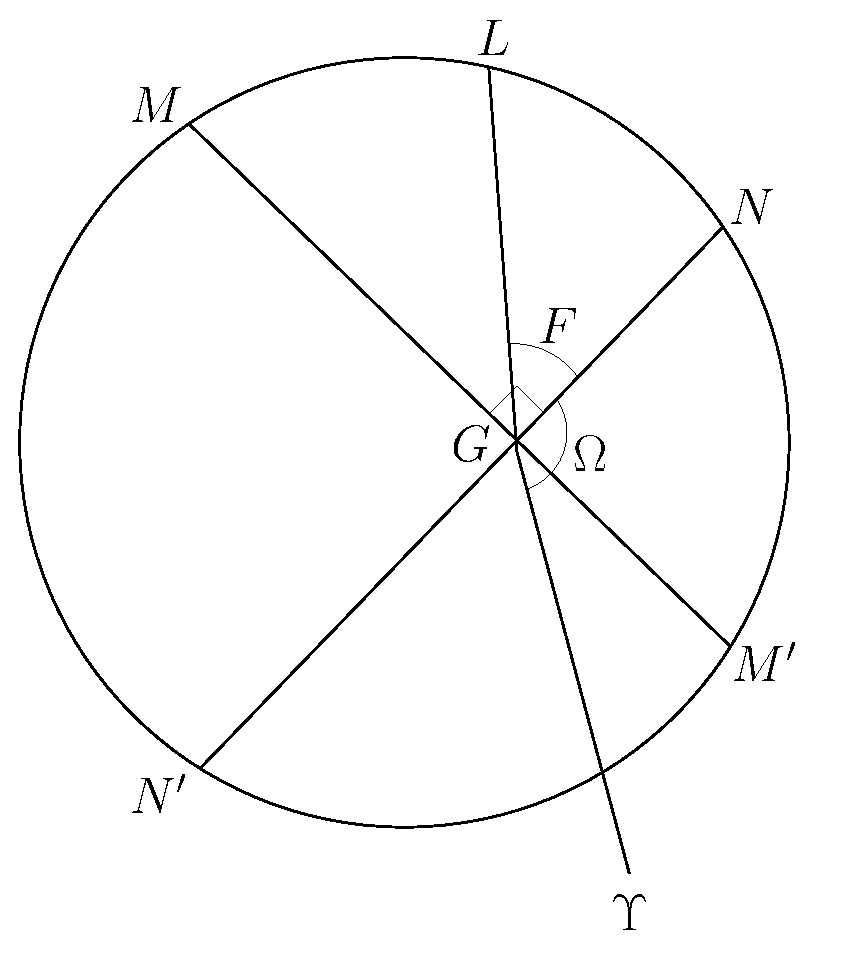
\includegraphics[height=3in]{epsfiles/moon.eps}}
\caption{The orbit of the Moon about the Earth.  Here, $G$, $L$, $N$, $N'$,   $\Omega$, $F$, and $\Upsilon$
represent the Earth, the Moon, the ascending node, the descending node, the longitude of the ascending node, the argument of latitude, and the vernal equinox, respectively. The view is from northern ecliptic pole. The Moon orbits counterclockwise.}\label{fmoon}
\end{figure}

\section{Determination of Ecliptic Latitude}
A model of the Moon's ecliptic latitude is needed in order to predict the
occurrence of solar and lunar eclipses. Figure~\ref{fmoon} shows the
Moon's orbit about the Earth. The plane of this orbit is fixed, but slightly tilted with
respect to the plane of the ecliptic (that is, the plane of the Sun's
apparent orbit about the Earth). Let the two planes intersect along the
line of nodes, $NGN'$. Here, $N$ is the point at which the orbit crosses the
ecliptic plane from south to north (in the direction of the Moon's orbital
motion), and is termed the {\em ascending node}. Likewise, $N'$ is the
point at which the orbit crosses the ecliptic plane from north to south,
and is called the {\em descending node}. Incidentally, the line of nodes must pass through point $G$, because the Earth is common to the ecliptic plane and the plane of the lunar orbit.
The angle, $\Omega$, subtended between
 the radius vector $G\Upsilon$, connecting the Earth to the vernal equinox,
and the line $GN$, is known as the {\em longitude of the ascending node}. Note, incidentally, that
the ascending node precesses in the opposite direction to the Moon's orbital motion
at the rate  $\breve{n}-n = 5.2954\times 10^{-2}\,^\circ$ per day, or $360^\circ$ in 18.6 years. 
This unusually large precession rate is another consequence of the Sun's strong perturbing influence on the
Moon's orbit.
Let the line $MGM'$ lie in the plane
of the Moon's orbit such that it is perpendicular to $NGN'$.
The inclination, $i$,  of the Moon's orbital plane is the angle
that $GM$ subtends with its projection onto the ecliptic plane. Likewise, the
Moon's ecliptic longitude, $\beta$, is the angle that $GL$ subtends with its
projection onto the ecliptic plane.
Simple geometry
yields $\sin\beta = \sin i\,\sin F$, where $F$ is the angle
between $GN$ and $GL$. This angle is termed the {\em argument of latitude.} 
Now, it is easily seen that $F \simeq \lambda-\Omega$, where $\lambda$
is the Moon's ecliptic longitude (that is, the angle subtended
between  $G\Upsilon$ and $GL$). Here, we are assuming that the orbital
inclination $i$ is relatively
small. The {\em mean argument of latitude}\/ is defined $\bar{F} = \bar{\lambda}-\Omega$. 
 Hence, our model for the Moon's ecliptic latitude becomes
\begin{align}
F &=\bar{F}+q_1+q_2+q_3+q_4+q_5,\\[0.5ex]
\sin\beta &= \sin i\,\sin F.\label{emoonlat}
\end{align}
The value of the lunar orbital inclination, $i$,  for the
J2000 epoch is specified in Table~\ref{tmoon}. The above model is capable of
matching NASA ephemeris data during the years 1995-2006 AD with
a mean error of $6'$, and a maximum error of $11'$.

The ecliptic latitude of the Moon can be calculated with the aid of Table~\ref{tmoonb}. The procedure for using this table is as follows:
\begin{enumerate}

 \item Determine the fractional Julian day number, $t$, corresponding to the date and time
at which the Moon's ecliptic latitude is to be calculated with the aid of Tables~\ref{kt1}--\ref{kt3}. Form $\Delta t = t-t_0$, where $t_0=2\,451\,545.0$ is the epoch. 

\item Calculate the lunar mean argument of latitude, $\bar{F}$, 
and the five lunar anomalies, $q_1$--$q_5$, using the procedure outlined earlier in this 
section.

\item Form the argument $F = \bar{F}+q_1+q_2+q_3+q_4+q_5$. Add as many multiples of $360^\circ$ to $F$ as is required to make it fall in the range
$0^\circ$ to $360^\circ$. Round $F$ to the nearest degree.

\item Enter Table~\ref{tmoonb} with the value of $F$
and take out the lunar ecliptic latitude, $\beta$. It is necessary to
interpolate if $F$ is odd.
\end{enumerate}

For example, we have already seen that at 00:00 UT on May 5, 2005 AD
the lunar mean argument of latitude, and
the lunar anomalies, were $\bar{F}=337.132^\circ$, and
$q_1=5.555^\circ$, $q_2=-0.663^\circ$, $q_3=-0.631^\circ$, $q_4=-0.139^\circ$,
and $q_5=0.086^\circ$, respectively. Hence, $F=\bar{F}+q_1+q_2+q_3+q_4+q_5
=337.132+5.555-0.663-0.631-0.139+0.086\simeq 341^\circ$. Thus, according to Table~\ref{tmoonb}, the ecliptic latitude
of the Moon at  00:00 UT on May 5, 2005 AD was $-1.680^\circ\simeq -1^\circ 41'$.

\begin{figure}
\centerline{\includegraphics[height=3in]{epsfiles/parallax.eps}}
\caption{The Moon, $L$, as viewed by a hypothetical observer, $C$,
at the center of the Earth,  and a real observer, $X$, on the
surface of the Earth.}\label{fpara}
\end{figure}

\section{Lunar Parallax}\label{spara}
Now, it turns out that the Moon is sufficiently close to the Earth that its position in the sky is
significantly modified by {\em parallax}. All of our previous analysis
applies to a hypothetical observer situated at the center of the Earth.
Consider a real observer situated on the Earth's surface. It can
be seen from Figure~\ref{fpara} that the altitude of the Moon is
$a'$ for the real observer, and $a$ for the hypothetical observer. Simple
trigonometry reveals that $a' = a-\delta a$, which implies that the real
observer sees the Moon at a  lower altitude than the hypothetical observer.
Let $R$ be the radius of the Earth, and $r$ the distance from the center
of the Earth to the Moon. More simple trigonometry yields
\begin{equation}
\sin \delta a = \frac{R}{r}\,\cos a'.
\end{equation}
Let us assume that the Moon's orbit is elliptical to first order in its
eccentricity. It follows, from Chapter~\ref{ckep}, that
\begin{equation}
r \simeq a_M\,(1 - e\,\cos M),
\end{equation}
where $a_M$, $e$, and $M$ are major radius, eccentricity, and mean
anomaly of the lunar orbit, respectively. Assuming that $\delta a$ is small, we
obtain
\begin{equation}\label{ea112}
\delta a \simeq \delta a_0\,\cos a\,(1+e\,\cos M),
\end{equation}
where $\delta a_0 = R/a_M = 0.0166=56.98'$ (because $R=6371$ km and $a_M=384\,399$ km). 

According to Equation~(\ref{ea112}), lunar parallax can be written in the form
\begin{equation}
\delta a = \delta (a)\,[1+\zeta (M)],
\end{equation}
where $a$, $a-\delta a$, and $M$ are the Moon's geocentric altitude (that is, the altitude seen from the center of the Earth), true
altitude, and mean anomaly, respectively. The functions $\delta(a)=\delta a_0\,\cos a$ and
$\zeta (M)= e\,\cos M$ are tabulated in Table~\ref{tmoonc}. It can be seen from the
table that lunar parallax increases with decreasing lunar altitude, reaching a maximum value of about $57'$ when the Moon is close to the horizon.
For example, if $a=44^\circ 00'$ and $M=100^\circ$ then Table~\ref{tmoonc}
yields $\delta = 41.050'$ and $\zeta =- 0.00953$. Hence, $\delta a = 41.050\,(1-0.00953) \simeq 41'$, and the true altitude of the Moon becomes
$43^\circ 19'$. 

\begin{figure}
\centerline{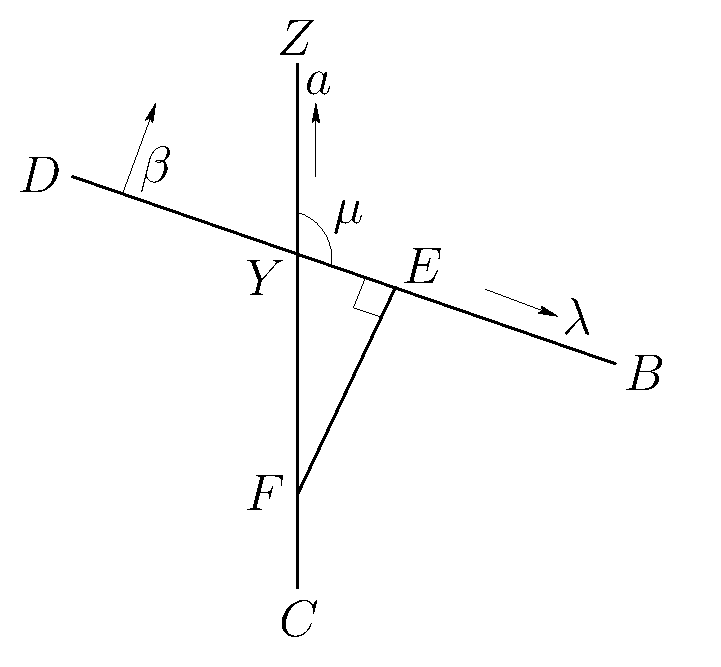
\includegraphics[height=3in]{epsfiles/para.eps}}
\caption{ Parallactic shifts in the Moon's ecliptic longitude and latitude.}\label{fpara1}
\end{figure}

It now remains to investigate how parallax affects the Moon's ecliptic
longitude and latitude. Figure~\ref{fpara1} shows a detail of Figure~\ref{f11}. Point $Y$ is the Moon's geocentric position on the celestial sphere. $DB$ is a line passing through this point
that is parallel to the local ecliptic circle, whereas $ZC$ is a small section of an
altitude circle passing through $Y$. The angle subtended between the ecliptic and the altitude circle is the parallactic angle, $\mu$. Let $F$ be the true position of the Moon.
It follows that $\delta a = YF$. The changes in the Moon's ecliptic longitude
and latitude are $\delta\lambda = YE$ and  $-\delta\beta = EF$, respectively. Here, we are considering the case where   increasing 
altitude corresponds to  increasing ecliptic latitude.
Assuming that the arcs $\delta a$, $\delta\lambda$, and $\delta\beta$ are
all fairly small, the triangle $YEF$ can be treated as a plane triangle.
Hence, we obtain
\begin{align}\label{epara1}
\delta\lambda &= - \delta a\,\cos\mu,\\[0.5ex]
\delta\beta &= - \delta a\,\sin\mu.\label{epara2}
\end{align}
As is easily demonstrated, the previous formulae also apply to the case in which increasing  altitude corresponds
to  decreasing  ecliptic latitude.

For example, consider a day on which the geocentric ecliptic longitude  and mean anomaly
of the Moon are $\lambda=210^\circ$ (that is, 00SC00) and $M=90^\circ$, respectively. Suppose that the Moon is
viewed from an observation site located  at terrestrial latitude $+10^\circ$. 
The ``Scorpio'' entry in Table~\ref{tscorp} gives the Moon's geocentric altitude, $a$, as a function of time, as well as the
value of the parallactic angle $\mu$. Making use of this data,
in combination with Table~\ref{tmoonc} and Equations~(\ref{epara1}) and (\ref{epara2}), we can calculate the parallax-induced changes in the Moon's ecliptic
longitude and latitude as it transits the sky. 
Data from such a calculation is given in the table below. The first column specifies
time because the  Moon's upper transit (thus, $t=+1$ hrs.\ means one hour after  the
upper transit), the second column gives the Moon's geocentric altitude, the third column the parallactic angle, 
the
fourth column the decrease in the Moon's real altitude due to parallax, and the fifth and
sixth columns the parallax-induced changes in its ecliptic longitude and latitude, respectively. 
It can be seen that parallax causes the Moon's apparent location
 to shift by almost $2^\circ$ relative to the fixed stars as it transits the sky. Note that the
previous calculation is somewhat inaccurate because it does not take into account the Moon's motion along the
ecliptic (which can easily amount to $6^\circ$ during the course of a night).
However, the calculation does illustrate how the data contained in
Tables~\ref{ltxx}--\ref{ltyy}, in combination with the data in Table~\ref{tmoonc}, permits the parallax-induced shift in the Moon's ecliptic position
to be calculated for a wide range of different lunar phases,
observation sites, and observation times.

~\\
\begin{tabular}{r|ccccc}\centering
$t$ (hrs.) & $a $ & $\mu$ & $\delta a $ & $\delta\lambda $ & $\delta\beta$\\\hline
&&&\\[-1.75ex]
$-5.51$ & $00^\circ 00'$  & $190^\circ 22'$ & $57'$ &$+56'$ & $+10'$\\
$-5.00$ & $12^\circ 26'$ & $187^\circ 30'$ & $56'$ & $+55'$ & $+07'$\\
$-4.00$ & $26^\circ  37'$ & $183^\circ 07'$ & $51'$ & $+51'$&$+03'$\\
$-3.00$ & $40^\circ 23'$ & $176^\circ 40'$ & $43'$ &$+43'$ & $-03'$\\
$-2.00$ & $53^\circ 15'$ & $165^\circ 58'$ & $34'$ & $+33'$&$-08'$\\
$-1.00$ & $63^\circ 52'$ & $145^\circ 55'$ & $25'$ & $+21'$&$-14'$\\
$+0.00$ & $68^\circ 32'$ & $110^\circ 34'$ & $21'$ & $+07'$ & $-20'$\\
$+1.00$ & $63^\circ 52'$ & $075^\circ 13'$ & $25'$ & $-06'$&$-24'$\\
$+2.00$ & $53^\circ 15'$ & $055^\circ 11'$ & $34'$ & $-20'$&$-28'$\\
$+3.00$ & $40^\circ 23'$ & $044^\circ 29'$ & $43'$ & $-31'$&$-30'$\\
$+4.00$ & $26^\circ 37'$ & $038^\circ01'$ & $51'$ & $-40'$&$-32'$\\
$+5.00$& $12^\circ 26'$ & $033^\circ 39'$ & $56'$ & $- 46'$&$-31'$\\
$+5.51$ & $00^\circ 00'$ & $030^\circ 47'$ & $57'$ & $-49'$&$-29'$\\
\end{tabular}\\
~\\~\\~\\

\newpage
\begin{table}[h]
\begin{tabular}{cccccccc}
$e$ & $n(^\circ/{\rm day})$ &  $\tilde{n}(^\circ/{\rm day})$  & $\breve{n}(^\circ/{\rm day})$
& $ \bar{\lambda}_0(^\circ)$ & $M_0(^\circ)$ & $ F_0(^\circ)$ & $i(^\circ)$ \\\hline
0.054881 & 13.17639646 & 13.06499295& $13.22935027$ &
218.322 & 134.916 & 93.284& 5.161\\
\end{tabular}
\caption{Orbital elements of the Moon for the J2000 epoch (that is, 12:00 UT, January 1, 2000 AD,
which corresponds to $t_0 = 2\,451\,545.0$ JD).}\label{tmoon}
\end{table}

\clearpage
\begin{table}
\centering
\begin{tabular}{rrrr|rrrr}
$\Delta t$(JD)& $\Delta\bar{\lambda}(^\circ)$ &  $\Delta M(^\circ)$ & $\Delta \bar{F}(^\circ)$& $\Delta t$(JD) & $\Delta\bar{\lambda}(^\circ)$ & $\Delta M(^\circ)$ 
&$\Delta \bar{F}(^\circ)$\\ \hline
&&&&&&&\\[-1.75ex]
10\,000 &   3.965 & 329.930 & 173.503 & 1\,000 & 216.396 & 104.993 & 269.350\\
20\,000 &   7.929 & 299.859 & 347.005 & 2\,000 &  72.793 & 209.986 & 178.701\\
30\,000 &  11.894 & 269.788 & 160.508 & 3\,000 & 289.189 & 314.979 &  88.051\\
40\,000 &  15.858 & 239.718 & 334.011 & 4\,000 & 145.586 &  59.972 & 357.401\\
50\,000 &  19.823 & 209.648 & 147.513 & 5\,000 &   1.982 & 164.965 & 266.751\\
60\,000 &  23.788 & 179.577 & 321.016 & 6\,000 & 218.379 & 269.958 & 176.102\\
70\,000 &  27.752 & 149.506 & 134.519 & 7\,000 &  74.775 &  14.951 &  85.452\\
80\,000 &  31.717 & 119.436 & 308.022 & 8\,000 & 291.172 & 119.944 & 354.802\\
90\,000 &  35.681 &  89.366 & 121.524 & 9\,000 & 147.568 & 224.937 & 264.152\\
&&&&&&&\\
100 & 237.640 & 226.499 & 242.935 & 10 & 131.764 & 130.650 & 132.294\\
200 & 115.279 &  92.999 & 125.870 & 20 & 263.528 & 261.300 & 264.587\\
300 & 352.919 & 319.498 &   8.805 & 30 &  35.292 &  31.950 &  36.881\\
400 & 230.559 & 185.997 & 251.740 & 40 & 167.056 & 162.600 & 169.174\\
500 & 108.198 &  52.496 & 134.675 & 50 & 298.820 & 293.250 & 301.468\\
600 & 345.838 & 278.996 &  17.610 & 60 &  70.584 &  63.900 &  73.761\\
700 & 223.478 & 145.495 & 260.545 & 70 & 202.348 & 194.550 & 206.055\\
800 & 101.117 &  11.994 & 143.480 & 80 & 334.112 & 325.199 & 338.348\\
900 & 338.757 & 238.494 &  26.415 & 90 & 105.876 &  95.849 & 110.642\\
&&&&&&&\\
1 &  13.176 &  13.065 &  13.229 & 0.1 &   1.318 &   1.306 &   1.323\\
2 &  26.353 &  26.130 &  26.459 & 0.2 &   2.635 &   2.613 &   2.646\\
3 &  39.529 &  39.195 &  39.688 & 0.3 &   3.953 &   3.919 &   3.969\\
4 &  52.706 &  52.260 &  52.917 & 0.4 &   5.271 &   5.226 &   5.292\\
5 &  65.882 &  65.325 &  66.147 & 0.5 &   6.588 &   6.532 &   6.615\\
6 &  79.058 &  78.390 &  79.376 & 0.6 &   7.906 &   7.839 &   7.938\\
7 &  92.235 &  91.455 &  92.605 & 0.7 &   9.223 &   9.145 &   9.261\\
8 & 105.411 & 104.520 & 105.835 & 0.8 &  10.541 &  10.452 &  10.583\\
9 & 118.588 & 117.585 & 119.064 & 0.9 &  11.859 &  11.758 &  11.906\\
\end{tabular}
\caption{Mean motion of the Moon.  Here, $\Delta t = t-t_0$, $\Delta\bar{\lambda} = \bar{\lambda}-\bar{\lambda}_0$, $\Delta M = M - M_0$, and $\Delta\bar{F}= \bar{F}-\bar{F}_0$. 
At epoch  ($t_0 = 2\,451\,545.0$ JD), $\bar{\lambda}_0 = 218.322^\circ$, $M_0 = 134.916^\circ$,
and $\bar{F}_0 = 93.284^\circ$.}\label{tmoonm}
\end{table}

\newpage
\begin{table}\centering
\small{ \begin{tabular}{rrrrrr|rrrrrr}
Arg. ($^\circ$) & $q_1(^\circ)$  & $q_2(^\circ)$ & $q_3(^\circ)$ & $q_4(^\circ)$  & $q_5(^\circ)$ &
Arg. ($^\circ$) & $q_1(^\circ)$  & $q_2(^\circ)$ & $q_3(^\circ)$ & $q_4(^\circ)$  & $q_5(^\circ)$  \\\hline
&&&&&&&&&&&\\[-1.75ex]
000/(360) &  0.000 &  0.000 &  0.000 & $-$0.000 & $-$0.000 & 090/(270) &  6.289 &  1.327 & $-$0.044 & $-$0.160 & $-$0.119\\
002/(358) &  0.237 &  0.046 &  0.045 & $-$0.006 & $-$0.004 & 092/(268) &  6.268 &  1.326 & $-$0.090 & $-$0.160 & $-$0.119\\
004/(356) &  0.473 &  0.093 &  0.089 & $-$0.011 & $-$0.008 & 094/(266) &  6.239 &  1.324 & $-$0.136 & $-$0.160 & $-$0.119\\
006/(354) &  0.709 &  0.139 &  0.133 & $-$0.017 & $-$0.012 & 096/(264) &  6.203 &  1.320 & $-$0.182 & $-$0.159 & $-$0.119\\
008/(352) &  0.943 &  0.185 &  0.177 & $-$0.022 & $-$0.017 & 098/(262) &  6.160 &  1.314 & $-$0.226 & $-$0.159 & $-$0.118\\
010/(350) &  1.176 &  0.230 &  0.219 & $-$0.028 & $-$0.021 & 100/(260) &  6.109 &  1.307 & $-$0.270 & $-$0.158 & $-$0.118\\
012/(348) &  1.408 &  0.276 &  0.261 & $-$0.033 & $-$0.025 & 102/(258) &  6.051 &  1.298 & $-$0.313 & $-$0.157 & $-$0.117\\
014/(346) &  1.637 &  0.321 &  0.301 & $-$0.039 & $-$0.029 & 104/(256) &  5.986 &  1.288 & $-$0.354 & $-$0.156 & $-$0.116\\
016/(344) &  1.864 &  0.366 &  0.339 & $-$0.044 & $-$0.033 & 106/(254) &  5.915 &  1.276 & $-$0.394 & $-$0.154 & $-$0.115\\
018/(342) &  2.088 &  0.410 &  0.376 & $-$0.050 & $-$0.037 & 108/(252) &  5.836 &  1.262 & $-$0.432 & $-$0.153 & $-$0.114\\
020/(340) &  2.310 &  0.454 &  0.411 & $-$0.055 & $-$0.041 & 110/(250) &  5.751 &  1.247 & $-$0.468 & $-$0.151 & $-$0.112\\
022/(338) &  2.527 &  0.497 &  0.444 & $-$0.060 & $-$0.045 & 112/(248) &  5.660 &  1.230 & $-$0.502 & $-$0.149 & $-$0.111\\
024/(336) &  2.741 &  0.540 &  0.475 & $-$0.065 & $-$0.049 & 114/(246) &  5.562 &  1.212 & $-$0.533 & $-$0.147 & $-$0.109\\
026/(334) &  2.951 &  0.582 &  0.504 & $-$0.070 & $-$0.052 & 116/(244) &  5.458 &  1.193 & $-$0.562 & $-$0.144 & $-$0.107\\
028/(332) &  3.157 &  0.623 &  0.529 & $-$0.075 & $-$0.056 & 118/(242) &  5.348 &  1.172 & $-$0.589 & $-$0.142 & $-$0.106\\
030/(330) &  3.358 &  0.663 &  0.553 & $-$0.080 & $-$0.060 & 120/(240) &  5.233 &  1.149 & $-$0.613 & $-$0.139 & $-$0.103\\
032/(328) &  3.554 &  0.703 &  0.573 & $-$0.085 & $-$0.063 & 122/(238) &  5.111 &  1.125 & $-$0.634 & $-$0.136 & $-$0.101\\
034/(326) &  3.746 &  0.742 &  0.591 & $-$0.090 & $-$0.067 & 124/(236) &  4.985 &  1.100 & $-$0.652 & $-$0.133 & $-$0.099\\
036/(324) &  3.931 &  0.780 &  0.605 & $-$0.094 & $-$0.070 & 126/(234) &  4.853 &  1.074 & $-$0.667 & $-$0.130 & $-$0.097\\
038/(322) &  4.111 &  0.817 &  0.617 & $-$0.099 & $-$0.074 & 128/(232) &  4.716 &  1.046 & $-$0.678 & $-$0.126 & $-$0.094\\
040/(320) &  4.285 &  0.853 &  0.625 & $-$0.103 & $-$0.077 & 130/(230) &  4.575 &  1.017 & $-$0.687 & $-$0.123 & $-$0.092\\
042/(318) &  4.454 &  0.888 &  0.630 & $-$0.107 & $-$0.080 & 132/(228) &  4.428 &  0.986 & $-$0.693 & $-$0.119 & $-$0.089\\
044/(316) &  4.615 &  0.922 &  0.632 & $-$0.111 & $-$0.083 & 134/(226) &  4.277 &  0.955 & $-$0.695 & $-$0.115 & $-$0.086\\
046/(314) &  4.770 &  0.955 &  0.631 & $-$0.115 & $-$0.086 & 136/(224) &  4.122 &  0.922 & $-$0.694 & $-$0.111 & $-$0.083\\
048/(312) &  4.919 &  0.986 &  0.627 & $-$0.119 & $-$0.089 & 138/(222) &  3.963 &  0.888 & $-$0.689 & $-$0.107 & $-$0.080\\
050/(310) &  5.061 &  1.017 &  0.620 & $-$0.123 & $-$0.092 & 140/(220) &  3.799 &  0.853 & $-$0.682 & $-$0.103 & $-$0.077\\
052/(308) &  5.195 &  1.046 &  0.609 & $-$0.126 & $-$0.094 & 142/(218) &  3.632 &  0.817 & $-$0.671 & $-$0.099 & $-$0.074\\
054/(306) &  5.323 &  1.074 &  0.595 & $-$0.130 & $-$0.097 & 144/(216) &  3.462 &  0.780 & $-$0.657 & $-$0.094 & $-$0.070\\
056/(304) &  5.443 &  1.100 &  0.579 & $-$0.133 & $-$0.099 & 146/(214) &  3.288 &  0.742 & $-$0.640 & $-$0.090 & $-$0.067\\
058/(302) &  5.555 &  1.125 &  0.559 & $-$0.136 & $-$0.101 & 148/(212) &  3.111 &  0.703 & $-$0.620 & $-$0.085 & $-$0.063\\
060/(300) &  5.660 &  1.149 &  0.536 & $-$0.139 & $-$0.103 & 150/(210) &  2.931 &  0.663 & $-$0.597 & $-$0.080 & $-$0.060\\
062/(298) &  5.757 &  1.172 &  0.511 & $-$0.142 & $-$0.106 & 152/(208) &  2.748 &  0.623 & $-$0.571 & $-$0.075 & $-$0.056\\
064/(296) &  5.847 &  1.193 &  0.483 & $-$0.144 & $-$0.107 & 154/(206) &  2.562 &  0.582 & $-$0.542 & $-$0.070 & $-$0.052\\
066/(294) &  5.929 &  1.212 &  0.453 & $-$0.147 & $-$0.109 & 156/(204) &  2.375 &  0.540 & $-$0.511 & $-$0.065 & $-$0.049\\
068/(292) &  6.002 &  1.230 &  0.420 & $-$0.149 & $-$0.111 & 158/(202) &  2.184 &  0.497 & $-$0.477 & $-$0.060 & $-$0.045\\
070/(290) &  6.068 &  1.247 &  0.385 & $-$0.151 & $-$0.112 & 160/(200) &  1.992 &  0.454 & $-$0.442 & $-$0.055 & $-$0.041\\
072/(288) &  6.126 &  1.262 &  0.348 & $-$0.153 & $-$0.114 & 162/(198) &  1.798 &  0.410 & $-$0.404 & $-$0.050 & $-$0.037\\
074/(286) &  6.176 &  1.276 &  0.309 & $-$0.154 & $-$0.115 & 164/(196) &  1.603 &  0.366 & $-$0.364 & $-$0.044 & $-$0.033\\
076/(284) &  6.218 &  1.288 &  0.269 & $-$0.156 & $-$0.116 & 166/(194) &  1.406 &  0.321 & $-$0.322 & $-$0.039 & $-$0.029\\
078/(282) &  6.252 &  1.298 &  0.227 & $-$0.157 & $-$0.117 & 168/(192) &  1.207 &  0.276 & $-$0.279 & $-$0.033 & $-$0.025\\
080/(280) &  6.278 &  1.307 &  0.184 & $-$0.158 & $-$0.118 & 170/(190) &  1.008 &  0.230 & $-$0.235 & $-$0.028 & $-$0.021\\
082/(278) &  6.296 &  1.314 &  0.139 & $-$0.159 & $-$0.118 & 172/(188) &  0.807 &  0.185 & $-$0.189 & $-$0.022 & $-$0.017\\
084/(276) &  6.306 &  1.320 &  0.094 & $-$0.159 & $-$0.119 & 174/(186) &  0.606 &  0.139 & $-$0.143 & $-$0.017 & $-$0.012\\
086/(274) &  6.308 &  1.324 &  0.048 & $-$0.160 & $-$0.119 & 176/(184) &  0.404 &  0.093 & $-$0.095 & $-$0.011 & $-$0.008\\
088/(272) &  6.302 &  1.326 &  0.002 & $-$0.160 & $-$0.119 & 178/(182) &  0.202 &  0.046 & $-$0.048 & $-$0.006 & $-$0.004\\
090/(270) &  6.289 &  1.327 & $-$0.044 & $-$0.160 & $-$0.119 & 180/(180) &  0.000 &  0.000 & $-$0.000 & $-$0.000 & $-$0.000\\
\end{tabular}}
\caption{Anomalies of the Moon. The common argument corresponds to
$M$, $2\tilde{D}-M$, $\tilde{D}$, $M_S$, and $2\bar{F}$ for the case of
$q_1$, $q_2$, $q_3$, $q_4$, and $q_5$, respectively. If the argument is
in parenthesies then the anomalies are minus the values shown
in the table. }\label{tmoona}
\end{table}

\newpage
\begin{table}\centering
\small{ \begin{tabular}{crc}
$F (^\circ)$ & $\beta(^\circ)$ &
$F (^\circ)$ \\\hline
&&\\[-1.75ex]
000/180 &  0.000 & (180)/(360)\\
002/178 &  0.180 & (182)/(358)\\
004/176 &  0.360 & (184)/(356)\\
006/174 &  0.539 & (186)/(354)\\
008/172 &  0.718 & (188)/(352)\\
010/170 &  0.896 & (190)/(350)\\
012/168 &  1.073 & (192)/(348)\\
014/166 &  1.248 & (194)/(346)\\
016/164 &  1.422 & (196)/(344)\\
018/162 &  1.595 & (198)/(342)\\
020/160 &  1.765 & (200)/(340)\\
022/158 &  1.933 & (202)/(338)\\
024/156 &  2.099 & (204)/(336)\\
026/154 &  2.263 & (206)/(334)\\
028/152 &  2.423 & (208)/(332)\\
030/150 &  2.581 & (210)/(330)\\
032/148 &  2.735 & (212)/(328)\\
034/146 &  2.887 & (214)/(326)\\
036/144 &  3.034 & (216)/(324)\\
038/142 &  3.178 & (218)/(322)\\
040/140 &  3.319 & (220)/(320)\\
042/138 &  3.455 & (222)/(318)\\
044/136 &  3.587 & (224)/(316)\\
046/134 &  3.714 & (226)/(314)\\
048/132 &  3.837 & (228)/(312)\\
050/130 &  3.956 & (230)/(310)\\
052/128 &  4.070 & (232)/(308)\\
054/126 &  4.178 & (234)/(306)\\
056/124 &  4.282 & (236)/(304)\\
058/122 &  4.380 & (238)/(302)\\
060/120 &  4.473 & (240)/(300)\\
062/118 &  4.561 & (242)/(298)\\
064/116 &  4.643 & (244)/(296)\\
066/114 &  4.719 & (246)/(294)\\
068/112 &  4.790 & (248)/(292)\\
070/110 &  4.855 & (250)/(290)\\
072/108 &  4.913 & (252)/(288)\\
074/106 &  4.966 & (254)/(286)\\
076/104 &  5.013 & (256)/(284)\\
078/102 &  5.054 & (258)/(282)\\
080/100 &  5.088 & (260)/(280)\\
082/098 &  5.117 & (262)/(278)\\
084/096 &  5.139 & (264)/(276)\\
086/094 &  5.154 & (266)/(274)\\
088/092 &  5.164 & (268)/(272)\\
090/090 &  5.167 & (270)/(270)\\
\end{tabular}}
\caption{Ecliptic latitude of the Moon.  The latitude is minus the value shown
in the table if the argument is
in parenthesies. }\label{tmoonb}
\end{table}

\newpage
\begin{table}\centering
\small{ \begin{tabular}{rrrc}
Arg. ($^\circ$) & $\delta(')$~~ &  $100\,\zeta$ & Arg. ($^\circ$) \\\hline
&&&\\[-1.75ex]
000/360 & 57.067 &  5.488 & (180)/(180)\\
002/358 & 57.032 &  5.485 & (178)/(182)\\
004/356 & 56.928 &  5.475 & (176)/(184)\\
006/354 & 56.754 &  5.458 & (174)/(186)\\
008/352 & 56.511 &  5.435 & (172)/(188)\\
010/350 & 56.200 &  5.405 & (170)/(190)\\
012/348 & 55.820 &  5.368 & (168)/(192)\\
014/346 & 55.371 &  5.325 & (166)/(194)\\
016/344 & 54.856 &  5.276 & (164)/(196)\\
018/342 & 54.274 &  5.219 & (162)/(198)\\
020/340 & 53.625 &  5.157 & (160)/(200)\\
022/338 & 52.911 &  5.088 & (158)/(202)\\
024/336 & 52.133 &  5.014 & (156)/(204)\\
026/334 & 51.291 &  4.933 & (154)/(206)\\
028/332 & 50.387 &  4.846 & (152)/(208)\\
030/330 & 49.421 &  4.753 & (150)/(210)\\
032/328 & 48.395 &  4.654 & (148)/(212)\\
034/326 & 47.310 &  4.550 & (146)/(214)\\
036/324 & 46.168 &  4.440 & (144)/(216)\\
038/322 & 44.969 &  4.325 & (142)/(218)\\
040/320 & 43.716 &  4.204 & (140)/(220)\\
042/318 & 42.409 &  4.078 & (138)/(222)\\
044/316 & 41.050 &  3.948 & (136)/(224)\\
046/314 & 39.642 &  3.812 & (134)/(226)\\
048/312 & 38.185 &  3.672 & (132)/(228)\\
050/310 & 36.682 &  3.528 & (130)/(230)\\
052/308 & 35.134 &  3.379 & (128)/(232)\\
054/306 & 33.543 &  3.226 & (126)/(234)\\
056/304 & 31.911 &  3.069 & (124)/(236)\\
058/302 & 30.241 &  2.908 & (122)/(238)\\
060/300 & 28.533 &  2.744 & (120)/(240)\\
062/298 & 26.791 &  2.577 & (118)/(242)\\
064/296 & 25.016 &  2.406 & (116)/(244)\\
066/294 & 23.211 &  2.232 & (114)/(246)\\
068/292 & 21.378 &  2.056 & (112)/(248)\\
070/290 & 19.518 &  1.877 & (110)/(250)\\
072/288 & 17.635 &  1.696 & (108)/(252)\\
074/286 & 15.730 &  1.513 & (106)/(254)\\
076/284 & 13.806 &  1.328 & (104)/(256)\\
078/282 & 11.865 &  1.141 & (102)/(258)\\
080/280 &  9.910 &  0.953 & (100)/(260)\\
082/278 &  7.942 &  0.764 & (098)/(262)\\
084/276 &  5.965 &  0.574 & (096)/(264)\\
086/274 &  3.981 &  0.383 & (094)/(266)\\
088/272 &  1.992 &  0.192 & (092)/(268)\\
090/270 &  0.000 &  0.000 & (090)/(270)\\
\end{tabular}}
\caption{Parallax of the Moon. The  arguments of $\delta$ and $\zeta$ are $a$
and $M$, respectively.  $\delta$ and $\zeta$ take minus the values shown
in the table if their arguments are
in parenthesies. }\label{tmoonc}
\end{table}


\chapter{Lunar-Solar Syzygies and Eclipses}
% !TEX root = ../Almagest.tex

\section{Syzygies}
Let $\lambda_S$ and $\lambda_M$ represent the ecliptic longitudes
of the Sun and the Moon, respectively. The lunar-solar {\em elongation}\/  is defined
\begin{equation}
D = \lambda_M - \lambda_S.
\end{equation}
Because the  Moon is only visible because of light reflected from the Sun, there is a fairly obvious relationship between lunar-solar elongation and lunar
phase. See Figure~\ref{fphase}. For instance, a {\em new moon}\/ corresponds to 
$D = 0^\circ$, a {\em quarter moon}\/ to $D = 90^\circ$ or $270^\circ$, and a {\em full moon}\/ to $D = 180^\circ$. New moons and full moons are collectively known as lunar-solar {\em syzygies}. (From the Greek
συζυγία, meaning ``yoking together'' or conjuction.)

\begin{figure}[h]
\centerline{\includegraphics[height=3in]{epsfiles/phase.eps}}
\caption{The phases of the Moon.}\label{fphase}
\end{figure}

\section{Lunar-Solar Elongation Model}
We can determine the  lunar-solar elongation  by combining the solar and
lunar models described in the previous two chapters. Our elongation model is as
follows:
\begin{align}
\bar{D} &= \bar{\lambda}_M - \bar{\lambda}_S,\\[0.5ex]
q_1 &= 2\,e_M\,\sin M_M + 1.2379\,e^2\,\sin 2M_M,\\[0.5ex]
q_2 &= 0.4052\,e_M\,\sin (2\bar{D} - M_M),\\[0.5ex]
q_3 &= 0.2094\,e_M\,(\sin 2\bar{D} - 0.0527\,\sin \bar{D}),\\[0.5ex]
q_4 &= -(0.0589\,e_M+2\,e_S)\,\sin M_S - (5/4)\,e_S^{\,2}\,\sin 2 M_S,\\[0.5ex]
q_5&= -0.0364\,e_M\,\sin 2 \bar{F}_M,\\[0.5ex]
D &= \bar{D} + q_1+q_2+q_3+q_4+q_5.
\end{align}
Here, $e_S$, $M_S$,  and $\bar{\lambda}_S$  are the eccentricity, mean anomaly,  and mean longitude  of the Sun's apparent orbit about the Earth, respectively. Moreover, $e_M$,
$M_M$, $\bar{\lambda}_M$, and $\bar{F}_M$ are the eccentricity, 
mean anomaly, mean longitude, and mean argument of latitude of
the Moon's orbit, respectively.

The lunar-solar elongation can be calculated with the aid of Tables~\ref{telon} and \ref{telona}.
Table~\ref{telon} allows the mean lunar-solar elongation, $\bar{D}$, the mean lunar
argument of latitude, $\bar{F}_M$, the mean anomaly of the Sun, $M_S$,
and the mean anomaly of the Moon, $M_M$, to be determined as functions of time.
Table~\ref{telona} specifies the anomalies $q_1$--$q_5$ as functions of their
various arguments.

Tables~\ref{telon} and \ref{telona} contain equivalent information to that contained in the ``Table of conjunctions" (Συνόδων κανόνιον) and the ``Table of full moons" (Πανσελήνων κανόνιον)
that appear in Section~3 of Book~VI of the Almagest.

\section{Determination of Lunar-Solar Elongation}\label{sxxc}
The procedure for using Tables~\ref{telon} and \ref{telona}  to determine the lunar-solar elongation is as follows:
\begin{enumerate}

 \item Determine the fractional Julian day number, $t$, corresponding to the date and time
at which the lunar-solar elongation is to be calculated with the aid of Tables~\ref{kt1}--\ref{kt3}. Form $\Delta t = t-t_0$, where $t_0=2\,451\,545.0$ is the epoch. 

\item Enter Table~\ref{telon} with the digit for each power of 10
in ${\Delta} t$ and take out the corresponding values of $\Delta \bar{D}$, $\Delta \bar{F}_M$,
 $\Delta M_S$, and $\Delta M_M$. If $\Delta t$ is negative then the 
values are minus those shown in the table.
The value of the mean lunar-solar elongation, $\bar{D}$, is the
sum of all the $\Delta\bar{D}$ values plus the value of $\bar{D}$ at the epoch.
Likewise, the value of the mean lunar argument of latitude, $\bar{F}_M$, is the
sum of all the $\Delta\bar{F}_M$ values plus the value of $\bar{F}_M$ at the epoch. Moreover, the value of the solar mean  anomaly, $M_S$, is
the sum of all the $\Delta M_S$ values plus the value of $M_S$ at the epoch. Finally, the value
of the lunar mean anomaly, $M_M$, is the
sum of all the $\Delta M_M$ values plus the value of $M_M$ at the epoch. 
Add as many multiples of $360^\circ$ to $\bar{D}$, $\bar{F}_M$, $M_S$, and $M_M$
as is required to make them all fall in the range $0^\circ$ to $360^\circ$. 

\item Form the five arguments $a_1=M_M$, $a_2=2\bar{D} - M_M$, $a_3=\bar{D}$, $a_4 = M_S$, $a_5=2\bar{F}_M$. Add as
many multiples of $360^\circ$ to the arguments as is required to make them all fall in the range
$0^\circ$ to $360^\circ$. Round each argument to the nearest degree.

\item Enter Table~\ref{telona} with the value of each of the five arguments $a_1$--$a_5$ and take out the
value of each of the five corresponding anomalies $q_1$--$q_5$. It is necessary to interpolate if the arguments are odd.

\item The lunar-solar elongation is given by $D=\bar{D} + q_1+q_2+q_3+q_4+q_5$.
If necessary, convert $D$ into an angle in the range $0^\circ$ to $360^\circ$. 
The decimal fraction can be converted into arc minutes
using Table~\ref{lt6a}. 
\end{enumerate}

In order to facilitate the calculation of syzygies, the previous model has been used to contruct Table~\ref{tnewmoon}, which lists
the dates and fractional Julian day numbers of the first new moons of the years 1900--2099 CE. Two examples
of syzygy calculations are given in the following section. Incidentally, our model is capable of predicting the times of new moons and full moons to within 10 minutes. 

\section{Example Syzygy Calculations}
\noindent {\em Example 1}: Sixth new moon in 2004 AD:\\
~\\
From Table~\ref{tnewmoon}, the date of first new moon in 2004 AD is 2453026.4 JD. Now, the
lunar-solar elongation increases at the mean rate $n_M - n_S = 13.17639646-0.98564735=12.1907491^\circ$ per day, or
$360^\circ$ in $29.53$ days; the latter  time period is known as a synodic month. Hence, a rough estimate for the
date of the sixth new moon in 2004 AD is five synodic months after that of the first: that is, $2453026.4
+ 5\times 29.53\simeq 2453174.1$ JD. It follows that $\Delta t = 2453174.1-2451545.0=1629.1$ JD. Let us calculate the lunar-solar elongation at this date.
From Table~\ref{telon}:\\
\begin{tabular}{rrrrr}
&&&&\\
$t$(JD) & $ \bar{D}(^\circ)$ & $\bar{F}_M(^\circ)$ & $M_S(^\circ)$ & $M_M(^\circ)$\\[-2ex]
&&&&\\
$+1\,000$ & $310.749$ & $269.350$ & $265.600$ & $104.993$\\
$+600$ & $114.449$ & $17.610$ & $231.360$ & $278.996$\\
$+20$ & $243.815$ & $264.587$ & $19.712$ & $261.300$\\
$+9$ & $109.717$ & $119.064$ & $8.870$ & $117.585$\\
$+.1$ & $1.219$ & $1.323$ & $0.099$ & $1.306$\\
Epoch & $297.864$ & $93.284$ & $357.588$ & $134.916$\\\cline{2-5}
&$1077.813$ & $765.218$ & $883.229$ & $899.096$\\\cline{2-5}
Modulus & $357.813$ & $45.218$ &$163.229$ & $179.096$\\ 
&&&\\
\end{tabular}\\
Thus,
$$
a_1=M_M\simeq 179^\circ,~~~a_2=2\bar{D}-M_M = 2\times 357.813-179.082\simeq 177^\circ,
$$ 
$$
a_3=\bar{D}\simeq 358^\circ,~~~a_4 = M_S\simeq 163^\circ,
$$ 
$$
a_5=2\bar{F}_M = 2\times 45.218\simeq 90^\circ.
$$
Table~\ref{telona} yields $$
q_1(a_1)=0.103^\circ,~~q_2(a_2)= 0.067^\circ,~~q_3(a_3) = -0.045^\circ,
$$
$$q_4(a_4)=-0.603^\circ,~~q_5(a_5)= -0.114^\circ.
$$
 Hence,
$$
D = \bar{D} + q_1+q_2+q_3+q_4+q_5=357.813+0.103+0.067-0.045-0.603-0.114\simeq
357.22^\circ.
$$
Now, the actual new moon takes place when $D=360.00^\circ$. Thus, a far better estimate for the date 
of the sixth new moon in 2004 AD is $2453174.10 +(360.00-357.22)/12.1907491= 2453174.33$ JD.
This corresponds to 19:55 UT on June 17th.

~\\
\noindent {\em Example 2}: Third full moon in 1982 AD\\
~\\
From Table~\ref{tnewmoon}, the fractional Julian day number of first new moon in 1982 AD is 2444994.7 JD, which
corresponds to January 25th. Because there is more than half a synodic month between this event and the
start of year, we conclude that the first full moon in 1982 AD took place before January 25th.  Hence, a rough estimate for the
date of the third full moon in 1982 AD is one and a half synodic months after that of the first new moon; that is, $2444994.7
+ 1.5\times 29.53\simeq 2445039.0$ JD. It follows that $\Delta t = 2445039.0 -2451545.0=-6506.0$ JD. Let us calculate the lunar-solar elongation at
this date.
From Table~\ref{telon}:\\
\begin{tabular}{rrrrr}
&&&&\\
$t$(JD) & $ \bar{D}(^\circ)$ & $\bar{F}_M(^\circ)$ & $M_S(^\circ)$ & $M_M(^\circ)$\\[-2ex]
&&&&\\
$-6\,000$ & $-64.495$ & $-176.102$ & $-153.601$ & $-269.958$\\
$-500$ & $-335.375$ & $-134.675$ & $-132.800$ & $-52.496$\\
$-6$ & $-73.144$ & $-79.376$ & $-5.914$ & $-78.390$\\
Epoch & $297.864$ & $93.284$ & $357.588$ & $134.916$\\\cline{2-5}
&$-175.150$ & $-296.869$ & $65.273$ & $-265.928$\\\cline{2-5}
Modulus & $184.131$ & $63.062$ &$65.273$ & $94.072$\\ 
&&&\\
\end{tabular}\\
Thus,

$$
a_1=M_M\simeq 94^\circ,~~~a_2=2\bar{D}-M_M = 2\times 184.850-94.072\simeq 276^\circ,
$$ 
$$
a_3=\bar{D}\simeq 185^\circ,~~~a_4 = M_S\simeq 65^\circ,
$$ 
$$
a_5=2\bar{F}_M = 2\times 63.062\simeq 126^\circ.
$$
Table~\ref{telona} yields $$
q_1(a_1)=6.244^\circ,~~q_2(a_2)= -1.267^\circ,~~q_3(a_3) = 0.118^\circ,
$$
$$q_4(a_4)=-1.918^\circ,~~q_5(a_5)= -0.093^\circ.
$$
 Hence,
$$
D = \bar{D} + q_1+q_2+q_3+q_4+q_5=184.850+6.244-1.267+0.118-1.918-0.093\simeq
187.93^\circ.
$$
Now, the actual full moon  takes place when $D=180.00^\circ$. Thus, a far better estimate for the date 
of the third full moon in 1982 AD is $2445039.0 +(180.00-187.93)/12.1907491= 2445038.35$ JD.
This corresponds to 20:04  UT on March 9th.

\section{Solar and Lunar Eclipses}
A {\em solar eclipse}---or, more accurately, a lunar-solar occultation---occurs
when the Moon blocks the light of the Sun. Clearly, this is
only possible at a new moon. See Figure~\ref{fphase}. On the other hand,
a {\em lunar eclipse}\/ occurs when the Moon falls into the
shadow of the Earth. Of course, this is only possible at a full moon. It follows that eclipses
can only take place at  lunar-solar syzygies.

In order to determine whether a particular lunar-solar syzygy coincides with an eclipse, we first need to calculate the angular radii of the
Sun, the Moon, and the Earth's shadow in the sky. Using the small angle approximation, the
angular radius of the  Sun is given by $\rho_S = R_S/r_S$, where
$R_S$ is the solar radius, and $r_S$ the Earth-Sun distance. However,
$r_S\simeq a_S\,(1-e_S\,\cos M_S)$, where $a_S$, $e_S$, and $M_S$
are the major radius, eccentricity, and mean anomaly of the Sun's apparent
orbit around the Earth, respectively. (See Chapter~\ref{ckep}.) Hence,
\begin{equation}
\rho_S \simeq \rho_{S\,0}\,(1+e_S\,\cos M_S),
\end{equation}
where $\rho_{S\,0}=R_S/a_S=6.960\times10^5\,{\rm km}/1.496\times 10^8\,{\rm km}\simeq 15.99'$.
Likewise, the angular radius of the Moon is
\begin{equation}
\rho_M\simeq  \rho_{M\,0}\,(1+e_M\,\cos M_M),
\end{equation}
where $\rho_{M\,0} = R_M/a_M =1743\,{\rm km}/384\,399\,{\rm km}\simeq 15.59'$. Here,
$R_M$, $a_M$, $e_M$, and $M_M$ are the radius of the Moon, and the major radius, eccentricity, and mean anomaly of the Moon's orbit, respectively.
As was shown in the previous chapter, lunar parallax causes the
angular position of the Moon in the sky to shift by up to
\begin{equation}
\delta_M = \frac{R_E}{r_M}= \delta_{M\,0}\,(1+e_M\,\cos M_M),
\end{equation}
where $\delta_{M\,0} = R_E/a_M = 6371\,{\rm km}/384\,399\,{\rm km}=56.98'$. Here, $R_E$ is the
radius of the Earth. Finally, simple trigonometry reveals that
the angular size of the Earth's shadow (that is, umbra) at the radius of the Moon's orbit is
\begin{equation}
\rho_U = \delta_M-\rho_S.
\end{equation}
This can be seen from Figure~\ref{fumbra}.
The radius of the umbra at the position of the Moon is $R_U = R_E-x=
R_E - r_M\,\rho_S$. Hence, the angular radius of the umbra is
$\rho_U = R_U/r_M = \delta_M-\rho_S$. Incidentally,
the identification of two of the angles in the figure with $\rho_S=R_S/r_S$ follows
because $R_S\gg R_E$.

\begin{figure}
\centerline{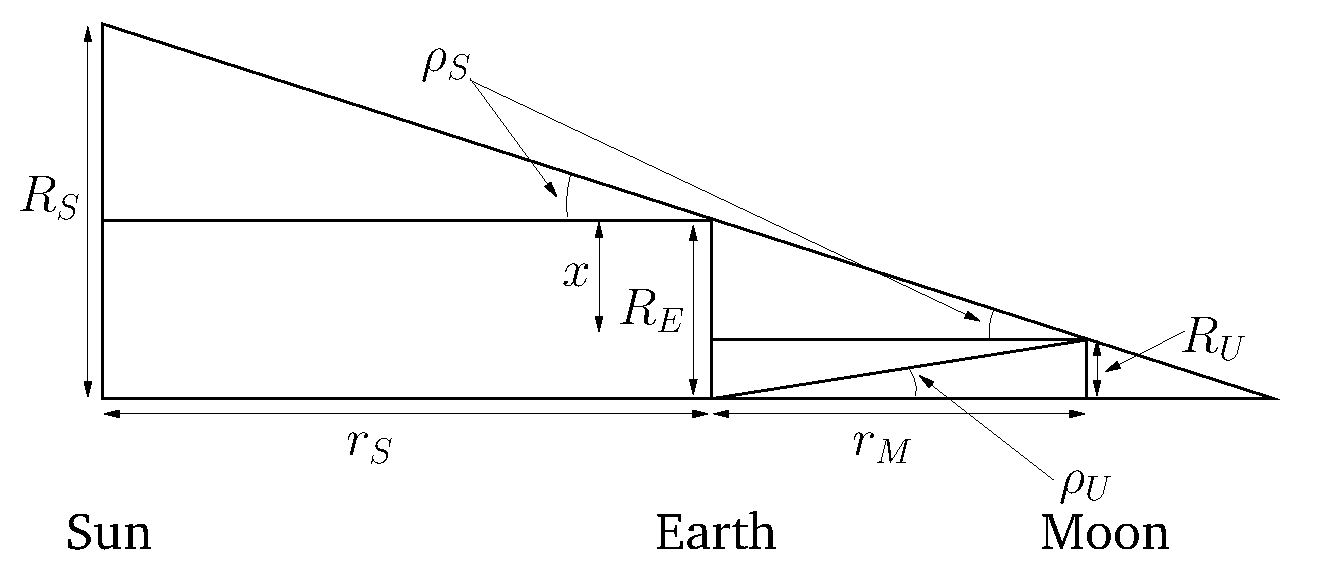
\includegraphics[height=2.5in]{epsfiles/umbra.eps}}
\caption{The Earth's umbra.}\label{fumbra}
\end{figure}

A solar eclipse does not take place every new moon,
nor a lunar eclipse every full moon, because of the inclination of the
Moon's orbit to the ecliptic plane, which causes the Moon to
pass either above or below the Sun, or the Earth's shadow, respectively, in the majority of cases. It follows
that the critical parameter that determines the occurrence of eclipses is
the ecliptic latitude of the Moon at syzygy, $\beta_{syz}$. Of course, once
the date  and time of a syzygy has been established, $\beta_{syz}$
can be calculated from Table~\ref{tmoonb}. However, the lunar argument of latitude, $F$, must first be determined using
\begin{equation}\label{moonla}
F = \bar{F}_M + q_1+q_2+q_3+q_{4'}+q_5,
\end{equation}
where $\bar{F}_M$ comes from Table~\ref{telon}, $q_1$, $q_2$, $q_3$, and $q_5$ are obtained from Table~\ref{telona},
and $q_{4'}$ is the $q_4$ from Table~\ref{tmoona}. For instance, we
have seen that for the third full moon of 1982 AD, $\bar{F}_M=63.062$, $M_S\simeq 65^\circ$, $q_1=6.244^\circ$, $q_2=-1.267^\circ$, $q_3=0.118^\circ$, and $q_5=-0.093^\circ$. According to Table~\ref{tmoona}, $q_{4'}(M_S) = -0.168^\circ$. Hence, $F =  \bar{F}_M + q_1+q_2+q_3+q_{4'}+q_5
=63.062+6.244-1.267+0.118-0.168-0.093=67.926\simeq 68^\circ$. 
It follows from Table~\ref{tmoonb} that $\beta_{syz} = 4.784^\circ\simeq 4^\circ 47'$. 

\begin{figure}
\centerline{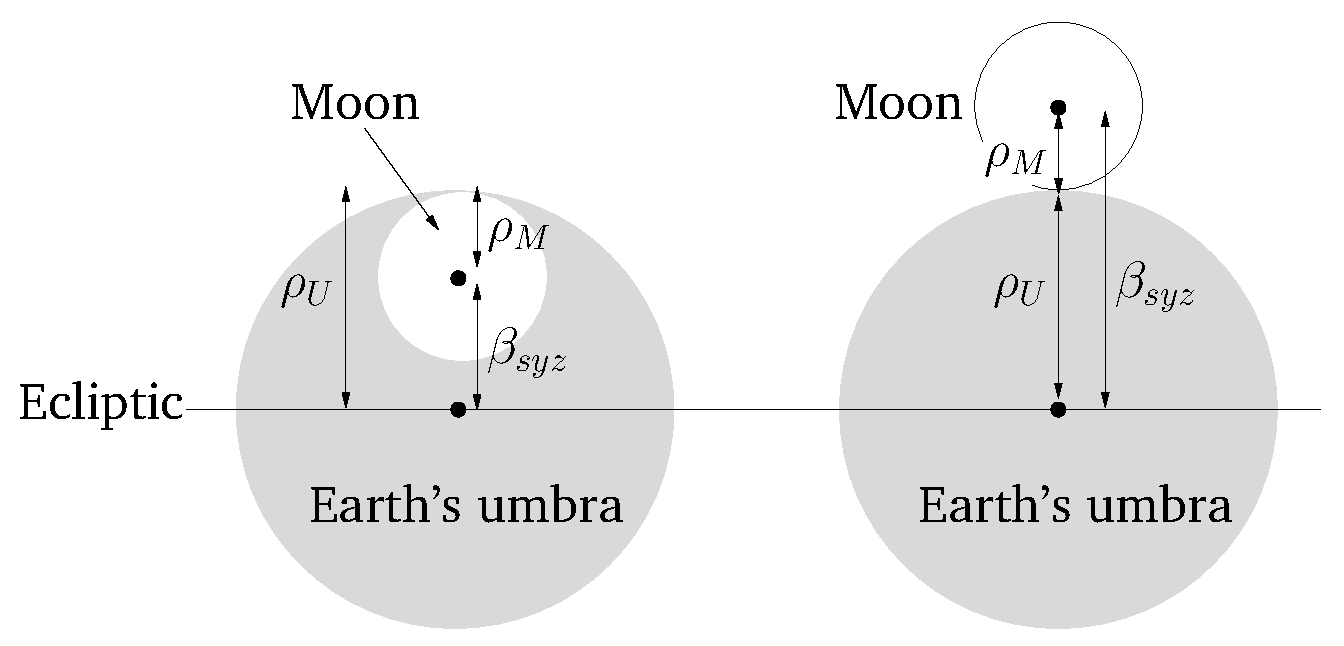
\includegraphics[height=2.5in]{epsfiles/totalm.eps}}
\caption{The limiting cases for a total lunar eclipse (left) and a partial lunar eclipse (right).}\label{fmoonec}
\end{figure}

The criterion for
a lunar eclipse is particularly simple, because it is not
complicated by lunar parallax. A {\em total lunar eclipse}, in which the Moon is
completely immersed in the Earth's shadow, must take place at a
full moon if $|\beta_{syz}| < \rho_U-\rho_M$ (see Figure~\ref{fmoonec}),
or equivalently
\begin{equation}
|\beta_{syz}| < \delta_M-\rho_M-\rho_S,
\end{equation}
and either a total or a {\em partial lunar eclipse}, in which the Moon is only
partially immersed in the Earth's shadow, must take place if
$ |\beta_{syz}| < \rho_U+\rho_M$ (see Figure~\ref{fmoonec}),
or  equivalently
\begin{equation}
|\beta_{syz}| < \delta_M+\rho_M-\rho_S.
\end{equation}
 Note that lunar eclipses are simultaneously
visible at all observation sites on the Earth for which the Moon is
above the horizon, because the Earth's shadow is larger than the Moon, and the relative position of the Moon and the Earth's shadow is not affected by parallax
(because both the Moon and the shadow are the same distance from the Earth).

 The criterion for a solar eclipse is modified by lunar parallax, which causes the angular position of the Moon relative to the Sun to shift by up to $\delta_M$ from its geocentric position. The amount of the shift
 depends on the observation site. However, a site can always be found
 at which the shift takes its maximum value in any particular direction.
 Note that the Sun has negligible parallax, because it is much farther away from the Earth than the Moon. Taking parallactic shifts into account, a {\em total solar eclipse}, in which the Sun is totally obscured by the Moon,
must take place if $\rho_M>\rho_S$ and
 \begin{equation}
 |\beta_{syz}| < \delta_M + \rho_M - \rho_S,
 \end{equation}
 an {\em annular solar eclipse}, in which all of the Sun apart from
 a thin outer ring is obscured by the Moon, must take place if
 $\rho_S>\rho_M$ and
 \begin{equation}
 |\beta_{syz}| < \delta_M +  \rho_S-\rho_M,
 \end{equation}
 and either a total, an annular,  or a {\em partial solar eclipse}, in which the
 Sun is only partially obscured by the Moon,  must take place if
 \begin{equation}
    |\beta_{syz}|< \delta_M + \rho_M + \rho_S.
  \end{equation}
As a consequence of lunar parallax, and the fact that the angular sizes of the Sun and Moon in the sky are very similar, solar eclipses are only visible in very localized regions of the Earth. Note, finally, that the previous criteria represent
necessary, but not sufficient, conditions for the occurrence of the various eclipses with which
they are associated. This is the case because the point of closest
approach of the Moon and the Earth's shadow, in the case of a
lunar eclipse, and the Moon and Sun, in the case of a solar eclipse, does
not necessarily occur exactly at the syzygy, due to the inclination
of the Moon's orbit to the ecliptic. However, because the said inclination
is fairly gentle, the previous criteria turn out to be very accurate
predictors of eclipses. 

The criterion for a total lunar eclipse can be written $|\beta_{syz}|< \beta_{Mt}$, where
\begin{equation}\label{elt}
\beta_{Mt} = 25.41' + \delta\beta_1(M_M)-\delta\beta_2 (M_M)-\delta\beta_3(M_S).%\label{ae137}
\end{equation}
Here, the functions $\delta\beta_1=\delta_{M\,0}\,e_M\,\cos M_M$, $\delta\beta_2= \rho_{M\,0}\,e_M\,\cos M_M$, and $\delta\beta_3=\rho_{S\,0}\,e_S\,\cos M_S$
are tabulated in Table~\ref{tsyzb}. The criterion for any type of
lunar eclipse becomes $|\beta_{syz}|< \beta_{M}$, where
\begin{equation}\label{elp}
\beta_{M} = 56.59' +  \delta\beta_1(M_M)+\delta\beta_2 (M_M)-\delta\beta_3(M_S).
\end{equation}
The criterion for a total  solar eclipse can
be written $|\beta_{syz}|<\beta_{St}$ and $\beta_{St}>\beta_{Sa}$, where
\begin{equation}\label{est}
\beta_{St} = 56.59' +  \delta\beta_1(M_M)+\delta\beta_2 (M_M)-\delta\beta_3(M_S),
\end{equation}
and
\begin{equation}\label{esa}
\beta_{Sa} = 57.39' +  \delta\beta_1(M_M)-\delta\beta_2 (M_M)+\delta\beta_3(M_S),
\end{equation}
The criterion for an annular  solar eclipse is $|\beta_{syz}|<\beta_{Sa}$ and $\beta_{Sa}>\beta_{St}$.
Finally, 
the criterion for any
type of solar eclipse is $|\beta_{syz}|< \beta_{S}$, where
\begin{equation}\label{esp}
\beta_{S} = 88.57' +  \delta\beta_1(M_M)+\delta\beta_2 (M_M)+\delta\beta_3(M_S).%\label{ae140}
\end{equation}

\section{Example Eclipse Calculations}
Let us use our model to examine the lunar-solar syzygies of the year
1992 AD in order to see whether any of them were associated with solar or
lunar eclipses. The following  table  shows the dates and times of the new moons
of 1992 AD, calculated using the method described in Section~\ref{sxxc}. Also shown is the magnitude of the Moon's ecliptic latitude
at each syzygy, $|\beta_{syz}|$, calculated from 
Eqaution~(\ref{moonla}) and Table~\ref{tmoonb}, as well as the critical values of
this parameter for a general,  total, and annular solar eclipse. The latter are calculated from
Equations~(\ref{est})--(\ref{esp}) with the aid of Table~\ref{tsyzb}. It can be seen that
the criterion for a total solar eclipse (that is, $|\beta_{syz}|< \beta_{St}$ and $\beta_{St}>\beta_{Sa}$) is satisfied for the syzygy marked with a T,  the criterion for an annular solar eclipse (that is, $|\beta_{syz}|< \beta_{Sa}$ and $\beta_{Sa}>\beta_{St}$) for the syzygy marked with an A,
and
the criterion for a partial solar eclipse  (that is, $\beta_{St},\beta_{Sa}<|\beta_{syz}|< \beta_{S}$)  for the syzygy marked with a P. It is easily verified
that a total solar eclipse, an annular solar eclipse, and a partial solar eclipse did indeed
take place in 1992 AD at the dates and times indicated.\\
\begin{tabular}{ccccccc}
&&&&&&\\
Date & Time (UT) & $\beta_{S}(')$ & $\beta_{St}(')$ & $\beta_{Sa}(')$ & $|\beta_{syz}|(')$\\\hline
04/01/1992 &  23:15 & 84.5 & 53.0 & 54.9 & 023.0 & A\\
03/02/1992 &  18:58 & 84.4 & 53.0 & 54.9 & 182.7 &  \\
04/03/1992 &  13:14 & 85.4 & 53.9 & 55.5 & 286.6 &  \\
03/04/1992 &  04:52 & 87.1 & 55.3 & 56.5 & 306.0 &  \\
02/05/1992 &  17:39 & 89.0 & 57.0 & 57.7 & 239.7 &  \\
01/06/1992 &  03:55 & 90.7 & 58.5 & 58.7 & 110.0 &  \\
30/06/1992 &  12:18 & 92.0 & 59.6 & 59.4 & 047.1 & T\\
29/07/1992 &  19:35 & 92.7 & 60.2 & 59.9 & 191.6 &  \\
28/08/1992 &  02:43 & 92.8 & 60.3 & 59.9 & 287.0 &  \\
26/09/1992 &  10:44 & 92.1 & 59.7 & 59.5 & 306.6 &  \\
25/10/1992 &  20:38 & 90.9 & 58.6 & 58.8 & 241.5 &  \\
24/11/1992 &  09:14 & 89.1 & 57.1 & 57.7 & 106.1 &  \\
24/12/1992 &  00:49 & 87.1 & 55.3 & 56.5 & 062.3 & P\\
&&&&&&\\
\end{tabular}

The following table shows the dates and times of the full moons
of 1992 AD. Also shown is the magnitude of the Moon's ecliptic latitude
at each syzygy, as well as the critical values of
this parameter for a general and a total lunar eclipse. The latter are calculated from
Equations~(\ref{elp}) and (\ref{elt}), respectively, with the aid of Table~\ref{tsyzb}. It can be seen that
the criterion for a total lunar eclipse (that is, $|\beta_{syz}|< \beta_{Mt}$) is satisfied for the syzygy  marked with a T, whereas
the criterion for a partial lunar eclipse  (that is, $\beta_{Mt}<|\beta_{syz}|< \beta_{M}$) is satisfied for the syzygy marked with a P. It is easily verified
that a total lunar eclipse, and a partial lunar eclipse did indeed
take place in 1992 AD at the dates and times indicated.\\
\begin{tabular}{cccccc}
&&&&&\\
Date & Time (UT) & $\beta_{M}(')$ & $\beta_{Mt}(')$ & $|\beta_{syz}|(')$\\\hline
19/01/1992 &  21:25 & 60.3 & 27.4 & 107.1 &  \\
18/02/1992 &  07:51 & 60.0 & 27.2 & 242.8 &  \\
18/03/1992 &  18:07 & 59.1 & 26.7 & 307.2 &  \\
17/04/1992 &  04:43 & 57.7 & 26.0 & 284.3 &  \\
16/05/1992 &  16:14 & 56.1 & 25.1 & 184.2 &  \\
15/06/1992 &  05:06 & 54.5 & 24.3 & 035.8 & P\\
14/07/1992 &  19:18 & 53.4 & 23.7 & 121.6 &  \\
13/08/1992 &  10:26 & 52.9 & 23.4 & 247.3 &  \\
12/09/1992 &  02:02 & 53.2 & 23.6 & 307.5 &  \\
11/10/1992 &  17:49 & 54.3 & 24.2 & 283.0 &  \\
10/11/1992 &  09:17 & 55.9 & 25.1 & 177.1 &  \\
09/12/1992 &  23:47 & 57.7 & 26.0 & 018.4 & T\\
\end{tabular}

\section{Eclipse Statistics}
Consider a very large collection of lunar-solar syzygies. For such a collection,
we expect the lunar argument of latitude, $F$, the lunar mean anomaly, $M_M$,
and the solar mean anomaly, $M_S$, to be statistically independent of one another, and randomly distributed in
the range $0^\circ$ to $360^\circ$. Using this
insight, we can easily calculate the probability that a new moon is coincident with a
solar eclipse, or a full moon with a lunar eclipse, using Equation~(\ref{emoonlat})
and the criteria (\ref{elt})--(\ref{esp}).
For a new moon we find:\\
\begin{tabular}{lr}
&\\
Probability of total solar eclipse: &$4.2\%$\\
Probability of annular solar eclipse: &$7.7\%$\\
Probability of partial solar eclipse: &$6.6\%$\\
Probability of any solar eclipse:&$18.5\%$\\
&\\
\end{tabular}\\
 For a full moon we get:\\
\begin{tabular}{lr}
&\\
Probability of total lunar eclipse:& $5.2\%$\\
Probability of partial lunar eclipse: & $6.5\%$\\
Probability of any lunar eclipse:&$11.7\%$\\
&\\
\end{tabular}\\
Thus, we can see that, over a long  period of time, the ratio of the number of total/annular solar eclipses to the number of partial solar
eclipses is about 9/5, whereas the ratio of the number of partial 
lunar eclipses to the number of total lunar eclipses is approximately 5/4. Furthermore,
the ratio of the number of solar eclipses to the number of lunar eclipses
is about 11/7. Because there are 12.37 synodic months in a year, the
mean number of solar eclipses per year is approximately $12.37\times 0.185\simeq 2.3$,
whereas the mean number of lunar eclipses per year is about $12.37\times 0.117\simeq 1.4$. Clearly, solar eclipses are more  common that lunar
eclipses. On the other hand, at a given observation site on the Earth, lunar eclipses
are much more common than solar eclipses, because the former are visible
 over all regions of the Earth for which the Moon is above the horizon, whereas the latter are only visible in a very localized
region.

\section{Eclipse Cycles}
Now, $223$ synodic months corresponds to $6585.413$ days, which corresponds to $238.99$ anomalistic months and $242.00$ draconic months. 
This implies that if a solar eclipse takes place at a given new moon then, $223$ new moons later, the Moon's perigee and ascending node will be found in almost
the exact same positions, which 
 suggests that the Moon's ecliptic latitude, as well as $\beta_S$, $\beta_{St}$, and $\beta_{Sa}$, will take almost exactly the same values. Hence, another solar eclipse is almost
certain to happen $223$ new moons after a given eclipse. The same reasoning leads to the conclusion that if a lunar eclipse takes place at
a given full moon then another eclipse is almost certain to occur 223 full moons later. It can easily be demonstrated that there is no number of
synodic months less than $233$ that corresponds to integer numbers of both anomalistic and draconic months. Hence, the time period
of $223$ synodic months, which is (mistakenly) called the {\em saros}, is the minimum (almost) guaranteed period on which solar and lunar eclipses repeat. 

The following table gives details of a series of solar eclipses that take place at regular intervals of 223 new moons. \\
\begin{tabular}{ccccccc}
&&&&&&\\
Date & Time (UT) & $\beta_{S}(')$ & $\beta_{St}(')$ & $\beta_{Sa}(')$ & $|\beta_{syz}|(')$\\\hline
18/05/1920 & 06:20 & 92.4 & 60.0 & 59.7 & 63.9 & P\\
29/05/1938 & 13:56 & 92.4&  59.9&  59.6&  60.0 & P\\
08/06/1956 & 21:27 & 92.2  &59.8  &59.6&  55.8  &T\\
20/06/1974 &  04:53  & 92.1 & 59.7 & 59.5&  51.5  &T\\
30/06/1992 &  12:18 & 92.0 & 59.6 & 59.4 & 47.1 & T\\
11/07/2010 &  19:40 & 91.9 & 59.5 & 59.4 & 42.6&  T\\
22/07/2028 & 03:03  &91.7&  59.3 & 59.3 & 38.2 & T\\
 02/08/2046 &  10:26 & 91.6 & 59.2 & 59.2&  33.8&  T\\
  12/08/2064&  17:52 & 91.4 & 59.1 & 59.1 & 29.6 & A\\
  24/08/2082 & 01:21 & 91.2 & 58.9&  59.0&  25.7 & A\\
&&&&&&\\
\end{tabular}

Likewise, the following table gives details of a series of lunar eclipses that take place at regular intervals of 223 full moons. \\
\begin{tabular}{cccccc}
&&&&&\\
Date & Time (UT) & $\beta_{M}(')$ & $\beta_{Mt}(')$ & $|\beta_{syz}|(')$\\\hline
27/10/1920&  14:17&  58.3&  26.3&  14.0 & T\\
 07/11/1938&  22:32  &58.1 & 26.2&  15.5&  T\\
18/11/1956&  06:52 & 58.0 & 26.1&  16.7&  T\\
29/11/1974&  15:18&  57.8&  26.1&  17.7 & T\\
09/12/1992 &  23:47 & 57.7 & 26.0 &18.4 & T\\
21/12/2010&  08:19 & 57.5&  25.9&  18.9 & T\\
31/12/2028&  16:52 & 57.4 & 25.8&  19.4&  T\\
12/01/2047 & 01:25 & 57.2&  25.7&  19.9 & T\\
22/01/2065 & 09:55&  57.1&  25.7&  20.4 & T\\
02/02/2083 &18:22 & 56.9&  25.6 &21.0 & T\\
\end{tabular}



\clearpage
\begin{table}
\centering
\begin{tabular}{rrrrr|rrrrr}
$\Delta t$(JD)& $\Delta \bar{D}(^\circ)$ &  $\Delta \bar{F}_M(^\circ)$ & $\Delta M_S(^\circ)$& $\Delta M_M (^\circ)$ & $\Delta t$(JD) & $\Delta \bar{D}(^\circ)$ & $\Delta \bar{F}_M(^\circ)$ 
&$\Delta M_S(^\circ)$ & $\Delta M_M(^\circ)$\\ \hline
&&&&&&&&&\\[-1.75ex]
10\,000 & 227.491 & 173.503 & 136.002 & 329.930 & 1\,000 & 310.749 & 269.350 & 265.600 & 104.993\\
20\,000 &  94.982 & 347.005 & 272.005 & 299.859 & 2\,000 & 261.498 & 178.701 & 171.200 & 209.986\\
30\,000 & 322.473 & 160.508 &  48.007 & 269.788 & 3\,000 & 212.247 &  88.051 &  76.801 & 314.979\\
40\,000 & 189.964 & 334.011 & 184.010 & 239.718 & 4\,000 & 162.996 & 357.401 & 342.401 &  59.972\\
50\,000 &  57.455 & 147.513 & 320.012 & 209.648 & 5\,000 & 113.746 & 266.751 & 248.001 & 164.965\\
60\,000 & 284.947 & 321.016 &  96.015 & 179.577 & 6\,000 &  64.495 & 176.102 & 153.601 & 269.958\\
70\,000 & 152.438 & 134.519 & 232.017 & 149.506 & 7\,000 &  15.244 &  85.452 &  59.202 &  14.951\\
80\,000 &  19.929 & 308.022 &   8.020 & 119.436 & 8\,000 & 325.993 & 354.802 & 324.802 & 119.944\\
90\,000 & 247.420 & 121.524 & 144.022 &  89.366 & 9\,000 & 276.742 & 264.152 & 230.402 & 224.937\\
&&&&&&&&&\\
100 & 139.075 & 242.935 &  98.560 & 226.499 & 10 & 121.907 & 132.294 &   9.856 & 130.650\\
200 & 278.150 & 125.870 & 197.120 &  92.999 & 20 & 243.815 & 264.587 &  19.712 & 261.300\\
300 &  57.225 &   8.805 & 295.680 & 319.498 & 30 &   5.722 &  36.881 &  29.568 &  31.950\\
400 & 196.300 & 251.740 &  34.240 & 185.997 & 40 & 127.630 & 169.174 &  39.424 & 162.600\\
500 & 335.375 & 134.675 & 132.800 &  52.496 & 50 & 249.537 & 301.468 &  49.280 & 293.250\\
600 & 114.449 &  17.610 & 231.360 & 278.996 & 60 &  11.445 &  73.761 &  59.136 &  63.900\\
700 & 253.524 & 260.545 & 329.920 & 145.495 & 70 & 133.352 & 206.055 &  68.992 & 194.550\\
800 &  32.599 & 143.480 &  68.480 &  11.994 & 80 & 255.260 & 338.348 &  78.848 & 325.199\\
900 & 171.674 &  26.415 & 167.040 & 238.494 & 90 &  17.167 & 110.642 &  88.704 &  95.849\\
&&&&&&&&&\\
1 &  12.191 &  13.229 &   0.986 &  13.065 & 0.1 &   1.219 &   1.323 &   0.099 &   1.306\\
2 &  24.381 &  26.459 &   1.971 &  26.130 & 0.2 &   2.438 &   2.646 &   0.197 &   2.613\\
3 &  36.572 &  39.688 &   2.957 &  39.195 & 0.3 &   3.657 &   3.969 &   0.296 &   3.919\\
4 &  48.763 &  52.917 &   3.942 &  52.260 & 0.4 &   4.876 &   5.292 &   0.394 &   5.226\\
5 &  60.954 &  66.147 &   4.928 &  65.325 & 0.5 &   6.095 &   6.615 &   0.493 &   6.532\\
6 &  73.144 &  79.376 &   5.914 &  78.390 & 0.6 &   7.314 &   7.938 &   0.591 &   7.839\\
7 &  85.335 &  92.605 &   6.899 &  91.455 & 0.7 &   8.534 &   9.261 &   0.690 &   9.145\\
8 &  97.526 & 105.835 &   7.885 & 104.520 & 0.8 &   9.753 &  10.583 &   0.788 &  10.452\\
9 & 109.717 & 119.064 &   8.870 & 117.585 & 0.9 &  10.972 &  11.906 &   0.887 &  11.758\\
\end{tabular}
\caption{Mean motion of the lunar-solar elongation.  Here, $\Delta t = t-t_0$, $\Delta \bar{D}= \bar{D}-\bar{D}_0$, $\Delta \bar{F}_M= \bar{F}_M-\bar{F}_{M\,0}$,  
$\Delta M_S = M_S - M_{S\,0}$, and $\Delta M_M= M_M-M_{M\,0}$. 
At epoch  ($t_0 = 2\,451\,545.0$ JD), $\bar{D}_0 = 297.864^\circ$, $\bar{F}_{M\,0} = 93.284^\circ$,
$M_{S\,0} = 357.588^\circ$, and $M_{M\,0} = 134.916^\circ$. }\label{telon}
\end{table}

\newpage
\begin{table}\centering
\small{ \begin{tabular}{crrrrr|crrrrr}
Arg. ($^\circ$) & $q_1(^\circ)$  & $q_2(^\circ)$ & $q_3(^\circ)$ & $q_4(^\circ)$  & $q_5(^\circ)$ &
Arg. ($^\circ$) & $q_1(^\circ)$  & $q_2(^\circ)$ & $q_3(^\circ)$ & $q_4(^\circ)$  & $q_5(^\circ)$  \\\hline
&&&&&&&&&&&\\[-1.75ex]
000(360) & $+0.000$ & $+0.000$ & $+0.000$ & $-0.000$ & $-0.000$ & 090(270) & $+6.289$ & $+1.274$ & $-0.035$ & $-2.100$ & $-0.114$\\
002(358) & $+0.234$ & $+0.044$ & $+0.045$ & $-0.075$ & $-0.004$ & 092(268) & $+6.270$ & $+1.273$ & $-0.081$ & $-2.097$ & $-0.114$\\
004(356) & $+0.468$ & $+0.089$ & $+0.089$ & $-0.149$ & $-0.008$ & 094(266) & $+6.244$ & $+1.271$ & $-0.126$ & $-2.092$ & $-0.114$\\
006(354) & $+0.702$ & $+0.133$ & $+0.133$ & $-0.224$ & $-0.012$ & 096(264) & $+6.210$ & $+1.267$ & $-0.171$ & $-2.084$ & $-0.114$\\
008(352) & $+0.934$ & $+0.177$ & $+0.177$ & $-0.298$ & $-0.016$ & 098(262) & $+6.169$ & $+1.262$ & $-0.216$ & $-2.074$ & $-0.113$\\
010(350) & $+1.165$ & $+0.221$ & $+0.219$ & $-0.372$ & $-0.020$ & 100(260) & $+6.120$ & $+1.255$ & $-0.259$ & $-2.061$ & $-0.113$\\
012(348) & $+1.394$ & $+0.265$ & $+0.261$ & $-0.445$ & $-0.024$ & 102(258) & $+6.065$ & $+1.246$ & $-0.302$ & $-2.046$ & $-0.112$\\
014(346) & $+1.622$ & $+0.308$ & $+0.301$ & $-0.517$ & $-0.028$ & 104(256) & $+6.002$ & $+1.236$ & $-0.343$ & $-2.028$ & $-0.111$\\
016(344) & $+1.847$ & $+0.351$ & $+0.339$ & $-0.589$ & $-0.032$ & 106(254) & $+5.932$ & $+1.225$ & $-0.382$ & $-2.008$ & $-0.110$\\
018(342) & $+2.069$ & $+0.394$ & $+0.376$ & $-0.661$ & $-0.035$ & 108(252) & $+5.856$ & $+1.212$ & $-0.420$ & $-1.986$ & $-0.109$\\
020(340) & $+2.288$ & $+0.436$ & $+0.411$ & $-0.731$ & $-0.039$ & 110(250) & $+5.772$ & $+1.197$ & $-0.456$ & $-1.961$ & $-0.108$\\
022(338) & $+2.504$ & $+0.477$ & $+0.444$ & $-0.801$ & $-0.043$ & 112(248) & $+5.683$ & $+1.181$ & $-0.490$ & $-1.933$ & $-0.106$\\
024(336) & $+2.717$ & $+0.518$ & $+0.475$ & $-0.869$ & $-0.047$ & 114(246) & $+5.586$ & $+1.164$ & $-0.521$ & $-1.904$ & $-0.105$\\
026(334) & $+2.925$ & $+0.559$ & $+0.504$ & $-0.936$ & $-0.050$ & 116(244) & $+5.484$ & $+1.145$ & $-0.550$ & $-1.872$ & $-0.103$\\
028(332) & $+3.130$ & $+0.598$ & $+0.530$ & $-1.003$ & $-0.054$ & 118(242) & $+5.376$ & $+1.125$ & $-0.577$ & $-1.838$ & $-0.101$\\
030(330) & $+3.329$ & $+0.637$ & $+0.553$ & $-1.067$ & $-0.057$ & 120(240) & $+5.261$ & $+1.103$ & $-0.600$ & $-1.801$ & $-0.099$\\
032(328) & $+3.525$ & $+0.675$ & $+0.573$ & $-1.131$ & $-0.061$ & 122(238) & $+5.141$ & $+1.081$ & $-0.621$ & $-1.763$ & $-0.097$\\
034(326) & $+3.715$ & $+0.712$ & $+0.591$ & $-1.193$ & $-0.064$ & 124(236) & $+5.016$ & $+1.056$ & $-0.639$ & $-1.723$ & $-0.095$\\
036(324) & $+3.900$ & $+0.749$ & $+0.606$ & $-1.253$ & $-0.067$ & 126(234) & $+4.885$ & $+1.031$ & $-0.654$ & $-1.680$ & $-0.093$\\
038(322) & $+4.079$ & $+0.784$ & $+0.618$ & $-1.312$ & $-0.070$ & 128(232) & $+4.748$ & $+1.004$ & $-0.666$ & $-1.636$ & $-0.090$\\
040(320) & $+4.253$ & $+0.819$ & $+0.626$ & $-1.370$ & $-0.074$ & 130(230) & $+4.607$ & $+0.976$ & $-0.675$ & $-1.589$ & $-0.088$\\
042(318) & $+4.421$ & $+0.853$ & $+0.632$ & $-1.425$ & $-0.077$ & 132(228) & $+4.461$ & $+0.947$ & $-0.681$ & $-1.541$ & $-0.085$\\
044(316) & $+4.582$ & $+0.885$ & $+0.634$ & $-1.479$ & $-0.080$ & 134(226) & $+4.310$ & $+0.917$ & $-0.683$ & $-1.491$ & $-0.082$\\
046(314) & $+4.737$ & $+0.917$ & $+0.633$ & $-1.531$ & $-0.082$ & 136(224) & $+4.155$ & $+0.885$ & $-0.682$ & $-1.439$ & $-0.080$\\
048(312) & $+4.886$ & $+0.947$ & $+0.629$ & $-1.581$ & $-0.085$ & 138(222) & $+3.996$ & $+0.853$ & $-0.678$ & $-1.385$ & $-0.077$\\
050(310) & $+5.028$ & $+0.976$ & $+0.622$ & $-1.629$ & $-0.088$ & 140(220) & $+3.832$ & $+0.819$ & $-0.671$ & $-1.330$ & $-0.074$\\
052(308) & $+5.163$ & $+1.004$ & $+0.612$ & $-1.674$ & $-0.090$ & 142(218) & $+3.665$ & $+0.784$ & $-0.660$ & $-1.274$ & $-0.070$\\
054(306) & $+5.291$ & $+1.031$ & $+0.598$ & $-1.718$ & $-0.093$ & 144(216) & $+3.493$ & $+0.749$ & $-0.647$ & $-1.215$ & $-0.067$\\
056(304) & $+5.412$ & $+1.056$ & $+0.582$ & $-1.760$ & $-0.095$ & 146(214) & $+3.319$ & $+0.712$ & $-0.630$ & $-1.156$ & $-0.064$\\
058(302) & $+5.525$ & $+1.081$ & $+0.562$ & $-1.799$ & $-0.097$ & 148(212) & $+3.141$ & $+0.675$ & $-0.610$ & $-1.095$ & $-0.061$\\
060(300) & $+5.631$ & $+1.103$ & $+0.540$ & $-1.836$ & $-0.099$ & 150(210) & $+2.959$ & $+0.637$ & $-0.588$ & $-1.033$ & $-0.057$\\
062(298) & $+5.730$ & $+1.125$ & $+0.515$ & $-1.871$ & $-0.101$ & 152(208) & $+2.775$ & $+0.598$ & $-0.562$ & $-0.969$ & $-0.054$\\
064(296) & $+5.821$ & $+1.145$ & $+0.488$ & $-1.903$ & $-0.103$ & 154(206) & $+2.589$ & $+0.559$ & $-0.534$ & $-0.905$ & $-0.050$\\
066(294) & $+5.904$ & $+1.164$ & $+0.458$ & $-1.933$ & $-0.105$ & 156(204) & $+2.399$ & $+0.518$ & $-0.503$ & $-0.839$ & $-0.047$\\
068(292) & $+5.979$ & $+1.181$ & $+0.425$ & $-1.961$ & $-0.106$ & 158(202) & $+2.207$ & $+0.477$ & $-0.470$ & $-0.773$ & $-0.043$\\
070(290) & $+6.047$ & $+1.197$ & $+0.391$ & $-1.986$ & $-0.108$ & 160(200) & $+2.014$ & $+0.436$ & $-0.435$ & $-0.705$ & $-0.039$\\
072(288) & $+6.107$ & $+1.212$ & $+0.354$ & $-2.009$ & $-0.109$ & 162(198) & $+1.818$ & $+0.394$ & $-0.398$ & $-0.637$ & $-0.035$\\
074(286) & $+6.158$ & $+1.225$ & $+0.316$ & $-2.029$ & $-0.110$ & 164(196) & $+1.620$ & $+0.351$ & $-0.358$ & $-0.568$ & $-0.032$\\
076(284) & $+6.202$ & $+1.236$ & $+0.275$ & $-2.047$ & $-0.111$ & 166(194) & $+1.421$ & $+0.308$ & $-0.318$ & $-0.499$ & $-0.028$\\
078(282) & $+6.238$ & $+1.246$ & $+0.234$ & $-2.062$ & $-0.112$ & 168(192) & $+1.221$ & $+0.265$ & $-0.275$ & $-0.429$ & $-0.024$\\
080(280) & $+6.266$ & $+1.255$ & $+0.191$ & $-2.075$ & $-0.113$ & 170(190) & $+1.019$ & $+0.221$ & $-0.231$ & $-0.358$ & $-0.020$\\
082(278) & $+6.287$ & $+1.262$ & $+0.147$ & $-2.085$ & $-0.113$ & 172(188) & $+0.816$ & $+0.177$ & $-0.186$ & $-0.287$ & $-0.016$\\
084(276) & $+6.299$ & $+1.267$ & $+0.102$ & $-2.093$ & $-0.114$ & 174(186) & $+0.613$ & $+0.133$ & $-0.141$ & $-0.215$ & $-0.012$\\
086(274) & $+6.303$ & $+1.271$ & $+0.057$ & $-2.098$ & $-0.114$ & 176(184) & $+0.409$ & $+0.089$ & $-0.094$ & $-0.144$ & $-0.008$\\
088(272) & $+6.300$ & $+1.273$ & $+0.011$ & $-2.100$ & $-0.114$ & 178(182) & $+0.205$ & $+0.044$ & $-0.047$ & $-0.072$ & $-0.004$\\
090(270) & $+6.289$ & $+1.274$ & $-0.035$ & $-2.100$ & $-0.114$ & 180(180) & $+0.000$ & $+0.000$ & $-0.000$ & $-0.000$ & $-0.000$\\
\end{tabular}}
\caption{Anomalies of the lunar-solar elongation. The common argument corresponds to
$M_M$, $2\bar{D}-M_M$, $\bar{D}$, $M_S$, and $2\bar{F}_M$ for the case of
$q_1$, $q_2$, $q_3$, $q_4$, and $q_5$, respectively. If the argument is
in parentheses then the anomalies are minus the values shown
in the table. }\label{telona}
\end{table}

\begin{table}
{\small
\begin{tabular}{cc|cc|cc|cc}
01/01/1900 &  2415021.08 &  18/01/1950 &  2433299.83 & 06/01/2000 &  2451550.25 23/01/2050 & 2469829.71\\
20/01/1901 &  2415405.11 &  07/01/1951 &  2433654.34 & 24/01/2001 &  2451934.05 12/01/2051 & 2470184.29\\
09/01/1902 &  2415759.38 &  26/01/1952 &  2434038.43 & 13/01/2002 &  2452288.07 02/01/2052 & 2470538.62\\
28/01/1903 &  2416143.19 &  15/01/1953 &  2434393.09 & 02/01/2003 &  2452642.35 19/01/2053 & 2470922.46\\
17/01/1904 &  2416497.16 &  05/01/1954 &  2434747.60 & 21/01/2004 &  2453026.37 08/01/2054 & 2471276.44\\
05/01/1905 &  2416851.27 &  24/01/1955 &  2435131.54 & 10/01/2005 &  2453381.00 27/01/2055 & 2471660.24\\
24/01/1906 &  2417235.21 &  13/01/1956 &  2435485.62 & 29/01/2006 &  2453765.10 16/01/2056 & 2472014.43\\
14/01/1907 &  2417589.74 &  30/01/1957 &  2435869.40 & 19/01/2007 &  2454119.67 05/01/2057 & 2472368.91\\
03/01/1908 &  2417944.41 &  19/01/1958 &  2436223.43 & 08/01/2008 &  2454473.98 24/01/2058 & 2472753.00\\
22/01/1909 &  2418328.51 &  09/01/1959 &  2436577.73 & 26/01/2009 &  2454857.82 14/01/2059 & 2473107.67\\
11/01/1910 &  2418682.99 &  28/01/1960 &  2436961.76 & 15/01/2010 &  2455211.81 03/01/2060 & 2473462.20\\
30/01/1911 &  2419066.90 &  16/01/1961 &  2437316.40 & 04/01/2011 &  2455565.88 21/01/2061 & 2473846.13\\
19/01/1912 &  2419420.96 &  06/01/1962 &  2437671.03 & 23/01/2012 &  2455949.82 10/01/2062 & 2474200.24\\
07/01/1913 &  2419774.94 &  25/01/1963 &  2438055.07 & 11/01/2013 &  2456304.31 29/01/2063 & 2474584.02\\
26/01/1914 &  2420158.78 &  14/01/1964 &  2438409.36 & 30/01/2014 &  2456688.40 18/01/2064 & 2474938.03\\
15/01/1915 &  2420513.11 &  02/01/1965 &  2438763.38 & 20/01/2015 &  2457043.06 06/01/2065 & 2475292.30\\
05/01/1916 &  2420867.70 &  21/01/1966 &  2439147.16 & 10/01/2016 &  2457397.57 25/01/2066 & 2475676.34\\
23/01/1917 &  2421251.82 &  10/01/1967 &  2439501.26 & 28/01/2017 &  2457781.50 15/01/2067 & 2476030.97\\
12/01/1918 &  2421606.44 &  29/01/1968 &  2439885.19 & 17/01/2018 &  2458135.59 05/01/2068 & 2476385.61\\
02/01/1919 &  2421960.85 &  18/01/1969 &  2440239.70 & 06/01/2019 &  2458489.57 23/01/2069 & 2476769.65\\
21/01/1920 &  2422344.72 &  07/01/1970 &  2440594.36 & 24/01/2020 &  2458873.41 12/01/2070 & 2477123.97\\
09/01/1921 &  2422698.73 &  26/01/1971 &  2440978.46 & 13/01/2021 &  2459227.70 01/01/2071 & 2477478.01\\
27/01/1922 &  2423082.50 &  16/01/1972 &  2441332.95 & 02/01/2022 &  2459582.27 20/01/2072 & 2477861.78\\
17/01/1923 &  2423436.61 &  04/01/1973 &  2441687.15 & 21/01/2023 &  2459966.37 08/01/2073 & 2478215.85\\
06/01/1924 &  2423791.03 &  23/01/1974 &  2442070.96 & 11/01/2024 &  2460321.00 27/01/2074 & 2478599.78\\
24/01/1925 &  2424175.11 &  12/01/1975 &  2442424.94 & 29/01/2025 &  2460705.03 16/01/2075 & 2478954.27\\
14/01/1926 &  2424529.78 &  01/01/1976 &  2442779.11 & 18/01/2026 &  2461059.32 06/01/2076 & 2479308.93\\
03/01/1927 &  2424884.36 &  19/01/1977 &  2443163.09 & 07/01/2027 &  2461413.35 24/01/2077 & 2479693.03\\
22/01/1928 &  2425268.34 &  09/01/1978 &  2443517.66 & 26/01/2028 &  2461797.14 14/01/2078 & 2480047.55\\
11/01/1929 &  2425622.51 &  28/01/1979 &  2443901.77 & 14/01/2029 &  2462151.23 03/01/2079 & 2480401.78\\
29/01/1930 &  2426006.29 &  17/01/1980 &  2444256.40 & 04/01/2030 &  2462505.61 22/01/2080 & 2480785.58\\
18/01/1931 &  2426360.28 &  06/01/1981 &  2444610.81 & 23/01/2031 &  2462889.68 10/01/2081 & 2481139.55\\
07/01/1932 &  2426714.48 &  25/01/1982 &  2444994.70 & 12/01/2032 &  2463244.34 28/01/2082 & 2481523.37\\
25/01/1933 &  2427098.47 &  14/01/1983 &  2445348.72 & 30/01/2033 &  2463628.42 18/01/2083 & 2481877.66\\
15/01/1934 &  2427453.07 &  03/01/1984 &  2445702.73 & 20/01/2034 &  2463982.92 07/01/2084 & 2482232.22\\
05/01/1935 &  2427807.73 &  21/01/1985 &  2446086.61 & 09/01/2035 &  2464337.12 25/01/2085 & 2482616.34\\
24/01/1936 &  2428191.81 &  10/01/1986 &  2446441.01 & 28/01/2036 &  2464720.93 15/01/2086 & 2482970.98\\
12/01/1937 &  2428546.19 &  29/01/1987 &  2446825.07 & 16/01/2037 &  2465074.91 04/01/2087 & 2483325.42\\
01/01/1938 &  2428900.29 &  19/01/1988 &  2447179.73 & 05/01/2038 &  2465429.07 23/01/2088 & 2483709.31\\
20/01/1939 &  2429284.06 &  07/01/1989 &  2447534.31 & 24/01/2039 &  2465813.06 11/01/2089 & 2484063.34\\
09/01/1940 &  2429638.08 &  26/01/1990 &  2447918.31 & 14/01/2040 &  2466167.64 30/01/2090 & 2484447.11\\
27/01/1941 &  2430021.96 &  15/01/1991 &  2448272.49 & 02/01/2041 &  2466522.30 19/01/2091 & 2484801.19\\
16/01/1942 &  2430376.39 &  04/01/1992 &  2448626.47 & 21/01/2042 &  2466906.37 09/01/2092 & 2485155.57\\
06/01/1943 &  2430731.03 &  22/01/1993 &  2449010.28 & 11/01/2043 &  2467260.78 27/01/2093 & 2485539.64\\
25/01/1944 &  2431115.14 &  11/01/1994 &  2449364.46 & 30/01/2044 &  2467644.66 16/01/2094 & 2485894.30\\
14/01/1945 &  2431469.72 &  30/01/1995 &  2449748.45 & 18/01/2045 &  2467998.68 06/01/2095 & 2486248.90\\
03/01/1946 &  2431824.01 &  20/01/1996 &  2450103.03 & 07/01/2046 &  2468352.69 25/01/2096 & 2486632.91\\
22/01/1947 &  2432207.85 &  09/01/1997 &  2450457.69 & 26/01/2047 &  2468736.58 13/01/2097 & 2486987.12\\
11/01/1948 &  2432561.83 &  28/01/1998 &  2450841.76 & 15/01/2048 &  2469090.97 02/01/2098 & 2487341.11\\
29/01/1949 &  2432945.62 &  17/01/1999 &  2451196.16 & 04/01/2049 &  2469445.60 21/01/2099 & 2487724.89\\
\end{tabular}}
\caption{Dates and fractional Julian day numbers of the first new moons of the years 1900--2099 AD.}\label{tnewmoon}
\end{table}

\newpage
\begin{table}\centering
\small{ \begin{tabular}{rrrrc}
Arg. ($^\circ$) & $\delta\beta_1(')$ &  $\delta\beta_2(')$ &
 $\delta\beta_3(')$& Arg. ($^\circ$) \\\hline
&&&&\\[-1.75ex]
000/360 &  3.128 &  0.856 &  0.267 & (180)/(180)\\
002/358 &  3.126 &  0.855 &  0.267 & (178)/(182)\\
004/356 &  3.120 &  0.854 &  0.267 & (176)/(184)\\
006/354 &  3.111 &  0.851 &  0.266 & (174)/(186)\\
008/352 &  3.097 &  0.847 &  0.265 & (172)/(188)\\
010/350 &  3.080 &  0.843 &  0.263 & (170)/(190)\\
012/348 &  3.059 &  0.837 &  0.261 & (168)/(192)\\
014/346 &  3.035 &  0.830 &  0.259 & (166)/(194)\\
016/344 &  3.007 &  0.822 &  0.257 & (164)/(196)\\
018/342 &  2.975 &  0.814 &  0.254 & (162)/(198)\\
020/340 &  2.939 &  0.804 &  0.251 & (160)/(200)\\
022/338 &  2.900 &  0.793 &  0.248 & (158)/(202)\\
024/336 &  2.857 &  0.782 &  0.244 & (156)/(204)\\
026/334 &  2.811 &  0.769 &  0.240 & (154)/(206)\\
028/332 &  2.762 &  0.755 &  0.236 & (152)/(208)\\
030/330 &  2.709 &  0.741 &  0.231 & (150)/(210)\\
032/328 &  2.652 &  0.726 &  0.227 & (148)/(212)\\
034/326 &  2.593 &  0.709 &  0.222 & (146)/(214)\\
036/324 &  2.530 &  0.692 &  0.216 & (144)/(216)\\
038/322 &  2.465 &  0.674 &  0.211 & (142)/(218)\\
040/320 &  2.396 &  0.655 &  0.205 & (140)/(220)\\
042/318 &  2.324 &  0.636 &  0.199 & (138)/(222)\\
044/316 &  2.250 &  0.615 &  0.192 & (136)/(224)\\
046/314 &  2.173 &  0.594 &  0.186 & (134)/(226)\\
048/312 &  2.093 &  0.573 &  0.179 & (132)/(228)\\
050/310 &  2.010 &  0.550 &  0.172 & (130)/(230)\\
052/308 &  1.926 &  0.527 &  0.165 & (128)/(232)\\
054/306 &  1.838 &  0.503 &  0.157 & (126)/(234)\\
056/304 &  1.749 &  0.478 &  0.149 & (124)/(236)\\
058/302 &  1.657 &  0.453 &  0.142 & (122)/(238)\\
060/300 &  1.564 &  0.428 &  0.134 & (120)/(240)\\
062/298 &  1.468 &  0.402 &  0.125 & (118)/(242)\\
064/296 &  1.371 &  0.375 &  0.117 & (116)/(244)\\
066/294 &  1.272 &  0.348 &  0.109 & (114)/(246)\\
068/292 &  1.172 &  0.321 &  0.100 & (112)/(248)\\
070/290 &  1.070 &  0.293 &  0.091 & (110)/(250)\\
072/288 &  0.967 &  0.264 &  0.083 & (108)/(252)\\
074/286 &  0.862 &  0.236 &  0.074 & (106)/(254)\\
076/284 &  0.757 &  0.207 &  0.065 & (104)/(256)\\
078/282 &  0.650 &  0.178 &  0.056 & (102)/(258)\\
080/280 &  0.543 &  0.149 &  0.046 & (100)/(260)\\
082/278 &  0.435 &  0.119 &  0.037 & (098)/(262)\\
084/276 &  0.327 &  0.089 &  0.028 & (096)/(264)\\
086/274 &  0.218 &  0.060 &  0.019 & (094)/(266)\\
088/272 &  0.109 &  0.030 &  0.009 & (092)/(268)\\
090/270 &  0.000 &  0.000 &  0.000 & (090)/(270)\\
\end{tabular}}
\caption{Lunar-solar eclipse functions. The  arguments of $\delta\beta_1$, $\delta\beta_2$, and $\delta\beta_3$ are $M_M$, $M_M$, and $M_S$, respectively.  $\delta\beta_1$, $\delta\beta_2$, and  $\delta\beta_3$ take minus the values shown
in the table if their arguments are
in parentheses. }\label{tsyzb}
\end{table}



\chapter{The Superior Planets}\label{csup}
\section{Determination of Ecliptic Longitude}
Figure~\ref{vf7} compares and contrasts heliocentric and geocentric
models of the
motion  of a superior planet ({\em i.e.}, a planet which is further from the
sun than the earth), $P$,  as seen from the earth, $G$. The sun is
at $S$. In the heliocentric
model, we can write the earth-planet displacement vector, ${\bf P}$,
as the sum of the earth-sun displacement vector, ${\bf S}$, and
the sun-planet displacement vector, ${\bf P}'$.  The geocentric model,
which is entirely equivalent to the heliocentric model as far as
the {\em relative motion}\/ of the planet with respect to the
earth is concerned, and is much more convenient,  relies on the simple vector identity
\begin{equation}\label{ve2.15}
{\bf P} = {\bf S}+{\bf P}' \equiv{\bf P}'+{\bf S}.
\end{equation}
In other words, we can get from the earth to the planet by one of two
different routes. The first route corresponds to the heliocentric model, and
the second to the geocentric model.
In the latter model, ${\bf P}'$ gives the displacement of
the so-called {\em guide-point}, $G'$, from the earth. 
Since ${\bf P}'$ is also the displacement of the planet, $P$, from the
sun, $S$, it is clear that  $G'$ executes a
Keplerian orbit about the earth whose  elements are the
same as those of the orbit of the planet about the sun.
 The ellipse traced out by $G'$ is termed the {\em deferent}. The vector ${\bf S}$ gives
the displacement of the planet from the guide-point.
However, ${\bf S}$ is also the displacement of the sun from the earth.
Hence, it is clear that the planet, $P$,
executes a Keplerian orbit about the guide-point, $G'$, whose
 elements are the same as the sun's apparent orbit about the earth.
 The ellipse traced out by $P$ about $G'$ is termed the {\em epicycle}. 
\begin{figure}[h]
\epsfysize=2.75in
\centerline{\epsffile{epsfiles/figv7.eps}}
\caption[\em Heliocentric and geocentric models of the motion of a superior planet. ]{\em Heliocentric and geocentric models of the motion of a superior planet. Here, $S$ is the sun, $G$ the earth, and $P$ the planet. View is from the northern ecliptic pole.}\label{vf7}   
\end{figure}
 
\begin{figure}
\epsfysize=3in
\centerline{\epsffile{epsfiles/figv4.eps}}
\caption[\em Planetary longitude model.]{\em Planetary longitude model. View is from northern ecliptic pole. }\label{vf4}
\end{figure}

Figure~\ref{vf4} illustrates in more detail how the deferent-epicycle model
is used to determine the ecliptic longitude of a superior planet.
The planet $P$  orbits (counterclockwise) on a small Keplerian orbit $\Pi'PA'$
about  guide-point $G'$, which, in turn, orbits the earth, $G$, (counterclockwise) on a large
Keplerian orbit $\Pi G'A$. As has already been mentioned, the small orbit is termed the epicycle, and the large orbit  the deferent. Both orbits are assumed to lie in the plane of the ecliptic. This approximation does not
introduce a large error into our calculations because the orbital inclinations  of the visible planets to
the ecliptic plane are all fairly small.
 Let $C$, $A$, $\Pi$, $a$, $e$, $\varpi$,
and $T$ denote the geometric center, apocenter ({\em i.e.}, the point of
furthest distance from the central object), pericenter ({\em i.e.}, the
point of closest approach to the central object), major radius, eccentricity, longitude
of the pericenter, and true anomaly of the deferent, respectively. Let $C'$, $A'$, $\Pi'$, $a'$, $e'$, $\varpi'$, and $T'$ denote the corresponding
quantities for the epicycle.

\begin{figure}[h]
\epsfysize=2.5in
\centerline{\epsffile{epsfiles/figv5.eps}}
\caption{\em The triangle $GBP$.}\label{vf5xx}
\end{figure}

Let the line $GG'$ be produced, and let the perpendicular $PB$ be
dropped to it from $P$, as shown in Fig.~\ref{vf5xx}. The angle $\mu\equiv PG'B$
is termed the {\em epicyclic anomaly}\/ (see Fig.~\ref{vf5x}), and takes the form
\begin{equation}
\mu =T'+\varpi' - T - \varpi = \bar{\lambda}' + q' - \bar{\lambda}-q,
\end{equation}
where $\bar{\lambda}$ and $q$ are the mean longitude and equation of center for the
deferent, whereas $\bar{\lambda}'$ and $q'$ are the corresponding quantities for  the
epicycle---see Cha.~\ref{csun}. The epicyclic anomaly is generally written in the 
range $0^\circ$ to $360^\circ$. 
 The angle $\theta\equiv PGG'$ is termed the {\em equation of the epicycle}, and is usually written in the range $-180^\circ$ to $+180^\circ$.
It is clear from the figure that
\begin{equation}
\tan\theta = \frac{\sin\mu}{r/r'+ \cos\mu},
\end{equation}
where $r\equiv GG'$ and $r'\equiv G'P$ are the radial polar coordinates for the deferent and epicycle,
respectively. 
Moreover, according to Equation~(\ref{je22}), $r/r' = (a/a')\,z$, where
\begin{equation}\label{ezdef}
z = \frac{1-\zeta}{1-\zeta'},
\end{equation}
and
\begin{eqnarray}
\zeta &=& e\,\cos\,M -e^{\,2}\,\sin^2\,M,\\[0.5ex]
\zeta' &=& e'\cos\,M' -e'^{\,2}\sin^2\,M'
\end{eqnarray}
are termed {\em radial anomalies}. 
Finally, the ecliptic longitude of the planet is given by  (see Fig.~\ref{vf5x})
\begin{equation}
\lambda = \bar{\lambda} + q + \theta.
\end{equation}

Now, 
\begin{equation}
\theta(\mu,z) \equiv \tan^{-1}\left[ \frac{\sin\mu}{(a/a')\,z+ \cos\mu}\right]
\end{equation}
is a function of two variables, $\mu$ and $z$. It is impractical to tabulate
such a function directly. Fortunately, whilst $\theta(\mu,z)$
has a strong dependence on $\mu$, it only has a fairly weak dependence on $z$.
In fact, it is easily seen that $z$ varies between $z_{\rm min} = \bar{z} - \delta z$
and $z_{\rm max} = \bar{z}+\delta z$, where
\begin{eqnarray}
\bar{z} = \frac{1+e\,e'}{1-e'^{\,2}},\\[0.5ex]
\delta z = \frac{e+e'}{1-e'^{\,2}}.
\end{eqnarray}
Let us define
\begin{equation}
\xi = \frac{\bar{z}-z}{\delta z}.
\end{equation}
This variable takes the value $-1$ when $z=z_{\rm max}$, the value $0$ when
$z=\bar{z}$, and the value $+1$ when $z=z_{\rm min}$. 
Thus, using quadratic interpolation, we can write
\begin{equation}
\theta(\mu,z)\simeq \Theta_-(\xi)\,\delta\theta_-(\mu) + \bar{\theta}(\mu)
+ \Theta_+(\xi)\,\delta\theta_+(\mu),
\end{equation}
where
\begin{eqnarray}
\bar{\theta}(\mu)  &=& \theta(\mu,\bar{z}),\\[0.5ex]
\delta\theta_-(\mu) &=& \theta(\mu,\bar{z}) - \theta(\mu,z_{\rm max}),\\[0.5ex]
\delta\theta_+(\mu) &=& \theta(\mu,z_{\rm min}) - \theta(\mu,\bar{z}),
\end{eqnarray}
and
\begin{eqnarray}\label{ve52}
\Theta_-(\xi) &=& - (1/2)\,\xi\,(\xi-1),\\[0.5ex]
\Theta_+(\xi) &=&+ (1/2)\,\xi\,(\xi+1).\label{ve53}
\end{eqnarray}
This scheme allows us to avoid having to tabulate a
two-dimensional function, whilst ensuring that the exact value of $\theta(\mu,z)$ is obtained
when $z=\bar{z}$, $z_{\rm min}$, or $z_{\rm max}$. The above interpolation
scheme is very similar to that adopted by Ptolemy in the Almagest.

Our procedure for determining the ecliptic longitude of a superior planet is described below. It is assumed that the ecliptic longitude, $\lambda_S$, and the
radial anomaly, $\zeta_S$, of the sun have already been calculated. The latter quantity is tabulated as a function of the solar mean anomaly
in Table~\ref{lt6}. In the following, $a$, $e$, $n$, $\tilde{n}$, $\bar{\lambda}_0$, and $M_0$ represent  elements of the orbit of the planet in question
about the sun, and $e_S$  represents the eccentricity of the sun's apparent orbit
about the earth. (In general, the subscript $S$ denotes the sun.) In particular, $a$ is the major radius of the planetary orbit in
units in which the major radius of the sun's apparent orbit about the
earth is {\em unity}. The requisite elements for all of the superior planets at the J2000 epoch ($t_0=2\,451\,545.0$ JD)
are listed in Table~\ref{lt4}. The ecliptic longitude of a superior
planet is specified by the following formulae:
\begin{eqnarray}
\bar{\lambda}&=&  \bar{\lambda}_0 + n\,(t-t_0) ,\\[0.5ex]
M &=& M_0  +\tilde{n}\,(t-t_0),\\[0.5ex]
q&=& 2\,e\,\sin \,M + (5/4)\,e^2\,\sin\,2M,\label{ve3.8}\\[0.5ex]
\zeta &=& e\,\cos M - e^2\,\sin^2 M,\\[0.5ex]
\mu&=& \lambda_S - \bar{\lambda}-q,\\[0.5ex]
\bar{\theta} &=& \theta(\mu,\bar{z})\equiv \tan^{-1} \left(\frac{\sin\mu}{a\,\bar{z}+\cos\mu}\right),\\[0.5ex]
\delta\theta_- &=& \theta(\mu,\bar{z}) - \theta(\mu,z_{\rm max}),\\[0.5ex]
\delta\theta_+&=& \theta(\mu,z_{\rm min}) - \theta(\mu,\bar{z}),\\[0.5ex]
z &=& \frac{1-\zeta}{1-\zeta_S},\\[0.5ex]
\xi &=& \frac{\bar{z}-z}{\delta z},\\[0.5ex]
\theta  &=&\Theta_-(\xi)\,\delta\theta_-+ \bar{\theta}
+ \Theta_+(\xi)\,\delta\theta_+,\\[0.5ex]
\lambda &=&\bar{\lambda} + q+ \theta.
\end{eqnarray}
Here, $\bar{z} = (1+e\,e_S)/(1-e_S^{\,2})$, $\delta z = (e+e_S)/(1-e_S^{\,2})$, $z_{\rm min} = \bar{z}-\delta z$,
and $z_{\rm max} = \bar{z}+\delta z$.  The constants $\bar{z}$, $\delta z$, $z_{\rm min}$, and $z_{\rm max}$ 
for each of the superior planets are listed in Table~\ref{vtx}.  Finally, the functions $\Theta_\pm$ are  tabulated in Table~\ref{vty}.

For the case of Mars, the above formulae are capable of matching NASA ephemeris data during the years 1995--2006 CE
with a mean error of $3'$ and a maximum error of $14'$. For the case of Jupiter, the mean error is
$1.6'$ and the maximum error $4'$. Finally, for the case of Saturn, the mean error is $0.5'$ and the
maximum error $1'$. 

\section{Mars}
The ecliptic longitude of Mars can be determined with the aid of Tables~\ref{vt8}--\ref{vt10}. Table~\ref{vt8} allows
the mean longitude, $\bar{\lambda}$, and the mean anomaly, $M$, of Mars to be calculated as functions of
time. Next, Table~\ref{vt9} permits the equation of center, $q$, and the radial anomaly, $\zeta$, to
be determined as functions of the mean anomaly. Finally, Table~\ref{vt10} allows the quantities
$\delta\theta_-$, $\bar{\theta}$, and $\delta\theta_+$ to be calculated as functions of the epicyclic
anomaly, $\mu$. 

The procedure for using the tables is as follows:
\begin{enumerate}
\item Determine the fractional Julian day number, $t$, corresponding to the date and time
at which the ecliptic longitude is to be calculated with the aid of Tables~\ref{kt1}--\ref{kt3}. Form $\Delta t = t-t_0$, where $t_0=2\,451\,545.0$ is the epoch. 
\item Calculate the ecliptic longitude, $\lambda_S$, and radial anomaly,
$\zeta_S$, of the sun using the procedure set out in Sect.~\ref{ssun}.
\item Enter Table~\ref{vt8} with the digit for each power of 10
in ${\Delta} t$ and take out the corresponding values of $\Delta\bar{\lambda}$ and $\Delta M$. If $\Delta t$ is negative then the corresponding
values are also negative.
The value of the mean longitude, $\bar{\lambda}$, is the
sum of all the $\Delta\bar{\lambda}$ values plus the value of $\bar{\lambda}$ at the epoch. Likewise, the value of the mean anomaly, $M$, is
the sum of all the $\Delta M$ values plus the value of $M$ at the epoch. 
Add as many multiples of $360^\circ$ to $\bar{\lambda}$ and $M$
as is required to make them both fall in the range $0^\circ$ to $360^\circ$. Round $M$ to the nearest degree. 
\item Enter Table~\ref{vt9} with the value of $M$ and take out the
corresponding value of the equation of center, $q$, and the radial anomaly, $\zeta$. It is necessary to interpolate if $M$ is odd.
\item Form the epicyclic anomaly, $\mu = \lambda_S-\bar{\lambda}-q$. Add as many multiples of $360^\circ$ to $\mu$ as is required to make it fall in the range $0^\circ$ to $360^\circ$. Round $\mu$ to the nearest degree.
\item Enter Table~\ref{vt10} with the value of $\mu$ and take
out the corresponding values of $\delta\theta_-$, $\bar{\theta}$, and
$\delta\theta_+$. If $\mu > 180^\circ$ then it is necessary to make use
of the identities $\delta\theta_\pm(360^\circ - \mu) =-\delta\theta_\pm(\mu)$
and $\bar{\theta}(360^\circ - \mu) =-\bar{\theta}(\mu)$.
\item Form $z = (1-\zeta)/(1-\zeta_S)$.
\item Obtain the values of $\bar{z}$ and $\delta z$ from Table~\ref{vtx}.
Form $\xi = (\bar{z}-z)/\delta z$.
\item Enter Table~\ref{vty} with the value of $\xi$ and take out
the corresponding values of $\Theta_-$ and $\Theta_+$. If $\xi<0$ then
it is necessary to use the identities $\Theta_+(\xi)=-\Theta_-(-\xi)$
and $\Theta_-(\xi)=-\Theta_+(-\xi)$. 
\item Form the equation of the epicycle, $\theta = \Theta_-\,\delta\theta_-+ \bar{\theta}
+ \Theta_+\,\delta\theta_+$.
\item The ecliptic longitude, $\lambda$, is the sum of the mean longitude, $\bar{\lambda}$,  the equation of center, $q$, and the equation
of the epicycle, $\theta$. If necessary convert $\lambda$
into  an angle in the range $0^\circ$ to $360^\circ$. The decimal fraction can
be converted into arc minutes
using Table~\ref{lt6a}. Round to the nearest arc minute. The final result
can be written in terms of the signs of the zodiac using the table in Sect.~\ref{szod}.
\end{enumerate}
Two examples of this procedure are given below.

~\\
\noindent {\em Example 1}: May 5, 2005 CE, 00:00 UT:\\
~\\
From Sect.~\ref{ssun}, $t-t_0=1\,950.5$ JD, $\lambda_S= 44.602^\circ$, $M_S\simeq 120^\circ$. Hence, it follows from Table~\ref{lt6} that
$\zeta_S(M_S)= -8.56\times 10^{-3}$. Making use of
Table~\ref{vt8}, we find:\\
\begin{tabular}{rrr}
&&\\
$t$(JD) & $ \bar{\lambda}(^\circ)$ & $M(^\circ)$\\[-2ex]
&&\\
+1000 & $164.071$ & $164.021$\\
+900 & $111.664$ & $111.619$\\
+50 & $26.204$ & $26.201$\\
+.5 & $0.262$ & $0.262$\\
Epoch & $355.460$ & $19.388$\\\cline{2-3}
&$657.661$ & $321.491$\\\cline{2-3}
Modulus & $297.661$ & $321.491$\\ 
&&\\
\end{tabular}\\
Given that $M\simeq 321^\circ$, Table~\ref{vt9} yields 
$$
q(321^\circ)= -7.345^\circ,\mbox{\hspace{0.5cm}}\zeta(321^\circ)=6.912\times 10^{-2}.
$$
Thus, 
$$
\mu=\lambda_S - \bar{\lambda}-q = 44.602-297.661 + 7.345= 114.286\simeq
114^\circ,
$$
where we have rounded the epicylic anomaly to the nearest degree. It follows from Table~\ref{vt10}
that 
$$
\delta\theta_-(114^\circ) = 3.853^\circ,\mbox{\hspace{0.5cm}}\bar{\theta}(114^\circ)=39.209^\circ, \mbox{\hspace{0.5cm}}\delta\theta_+(114^\circ) = 4.612^\circ.
$$
Now,
$$ 
z= (1-\zeta)/(1-\zeta_S) = (1-6.912\times 10^{-2})/(1+8.56\times 10^{-3}) =
0.9230.
$$
However, from Table~\ref{vtx}, $\bar{z}= 1.00184$ and $\delta z = 0.11014$,
so
$$
\xi = (\bar{z}-z)/\delta z = (1.00184-0.9230)/0.11014 \simeq 0.72.
$$
According to Table~\ref{vty}, 
$$
\Theta_-(0.72) = 0.101, \mbox{\hspace{0.5cm}}\Theta_+(0.72) = 0.619,
$$
so
$$
\theta  = \Theta_-\,\delta\theta_- + \bar{\theta}+\Theta_+\,\delta\theta_+ = 0.101\times 3.853+39.209+0.619\times 4.612 = 42.453^\circ.
$$ 
Finally,
$$
\lambda=\bar{\lambda} + q + \theta= 297.661-7.345+42.453=332.769 \simeq 332^\circ 46'.
$$
Thus,
the ecliptic longitude of Mars at 00:00 UT on May 5, 2005 CE was 2PI46.

~\\
\noindent {\em Example 2}: December 25, 1800 CE, 00:00 UT:\\
~\\
From Sect.~\ref{ssun}, $t-t_0=-72,690.5$ JD, $\lambda_S= 273.055^\circ$, $M_S\simeq 354^\circ$. Hence, it follows from Table~\ref{lt6} that
$\zeta_S(M_S)= 1.662\times 10^{-2}$. Making use of
Table~\ref{vt8}, we find:\\
\begin{tabular}{rrr}
&&\\
$t$(JD) & $\bar{\lambda}(^\circ)$ & $ M(^\circ)$\\[-2ex]
&&\\
-70,000 & $-324.983$ & $-321.453$\\
-2,000 & $-328.142$ & $-328.042$\\
-600 & $-314.443$ & $-314.412$\\
-90 & $-47.166$ & $-47.162$\\
-.5 & $-0.262$ & $-0.262$\\
Epoch & $355.460$ & $19.388$\\\cline{2-3}
&$-659.536$ & $-991.943$\\\cline{2-3}
Modulus & $60.464$ & $88.057$\\
&&\\
\end{tabular}\\
Given that $M\simeq 88^\circ$, Table~\ref{vt9} yields 
$$
q(88^\circ)= 10.739^\circ, \mbox{\hspace{0.5cm}}\zeta(88^\circ)=-5.45\times 10^{-3},
$$
so
$$
\mu=\lambda_S - \bar{\lambda}-q = 273.055-60.464-10.739= 201.852\simeq202^\circ.
$$
It follows from Table~\ref{vt10}
that 
$$
\delta\theta_-(202^\circ) = -5.980^\circ,\mbox{\hspace{0.5cm}}\bar{\theta}(202^\circ)=-32.007^\circ,\mbox{\hspace{0.5cm}}\delta\theta_+(202^\circ) = -8.955^\circ.
$$
Now, 
$$
z= (1-\zeta)/(1-\zeta_S) = (1+5.45\times 10^{-3})/(1-1.662\times 10^{-2}) =
1.02244,
$$
so
$$
\xi = (\bar{z}-z)/\delta z = (1.00184-1.02244)/0.11014 \simeq -0.19.
$$ 
According to Table~\ref{vty}, 
$$
\Theta_-(-0.19) = -0.113, \mbox{\hspace{0.5cm}}
\Theta_+(-0.19) = -0.077,
$$
so
$$
\theta  = \Theta_-\,\delta\theta_- + \bar{\theta}+\Theta_+\,\delta\theta_+ = -0.113\times 5.980-32.007-0.077\times 8.955 = -30.642^\circ.
$$
Finally,
$$
\lambda=\bar{\lambda} + q + \theta= 60.464+10.739-30.642 = 40.561 \simeq 40^\circ 34'.
$$ 
Thus,
the ecliptic longitude of Mars at 00:00 UT on December 25, 1800 CE was 10TA34.

\begin{figure}[h]
\epsfysize=3in
\centerline{\epsffile{epsfiles/epicycle.eps}}
\caption[\em The geocentric orbit of a superior planet.]{\em The geocentric orbit of a superior planet. Here, $G$, $G'$, $P$,  $\mu$,  $\theta$, $\bar{\lambda}$, $q$, and $\Upsilon$ represent
the earth, guide-point, planet,  epicyclic anomaly, equation of the epicycle, mean longitude, equation of center, and spring equinox, respectively. View is
from northern ecliptic pole. Both $G'$ and $P$ orbit counterclockwise.}\label{vf5x}
\end{figure}

\section{Determination of Conjunction, Opposition, and Station Dates}
Figure~\ref{vf5x} shows the geocentric orbit of a superior planet. Recall that the vector $G'P$ is always {\em parallel}\/ to the vector connecting the earth to the sun. It follows that
a so-called {\em conjunction}, at which the sun lies
directly between the planet and the earth, occurs whenever the epicyclic anomaly, $\mu$, takes the value $0^\circ$. At
a conjunction, the planet is furthest from the earth, and has the same ecliptic longitude as the
sun, and is, therefore, invisible. Conversely, a so-called {\em opposition}, at which the earth lies directly between the planet and the sun, occurs whenever $\mu=180^\circ$. At an opposition, the planet is closest to the earth, and also directly opposite the 
sun in the sky, and, therefore, at its brightest. Now, a superior planet rotates around the epicycle at a
faster angular velocity than its guide-point rotates around the deferent. Moreover, both the planet and guide-point rotate
in the same direction. It follows that the planet is traveling {\em backward}\/ in the sky (relative to the direction
of its mean motion) at opposition. This phenomenon is called {\em retrograde motion}. The period of
retrograde motion begins and ends at  {\em stations}---so-called because when the planet reaches them
it appears to stand still in the sky for a few days whilst it reverses direction.

Tables~\ref{vt8}--\ref{vt10} can be used to determine the dates of the conjunctions, oppositions, and
stations of Mars. Consider the first conjunction after the epoch (January 1, 2000 CE). We can estimate the
time at which this event occurs by approximating the epicyclic anomaly as the so-called
{\em mean epicyclic anomaly}: 
$$
\mu \simeq \bar{\mu} = \bar{\lambda}_S-\bar{\lambda} = \bar{\lambda}_{0\,S}-\bar{\lambda}_0 +(n_S-n)\,(t-t_0) = 284.998 + 0.46157617\,(t-t_0).
$$
 We obtain
$$
t\simeq t_0 + (360-284.998)/0.46157617\simeq t_0 + 162\, {\rm JD}.
$$ 
A calculation of the epicyclic anomaly at this time, using Tables~\ref{vt8}--\ref{vt10}, yields $\mu=-9.583^\circ$. Now, the
actual conjunction occurs when $\mu=0^\circ$. Hence, our next estimate is 
$$
t\simeq t_0+162+9.583/0.46157617\simeq t_0 + 183\,{\rm JD}.
$$
A
calculation of the epicyclic anomaly at this time gives $0.294^\circ$. Thus, our final estimate is
$$
t=t_0 +183-0.294/0.461557617=t_0+182.4\, {\rm JD},
$$
which corresponds to July 1, 2000 CE.

Consider the first opposition of Mars after the epoch. Our first estimate of the time at which this
event takes place is 
$$
t\simeq t_0+(540-284.998)/0.46157617\simeq t_0 + 552\, {\rm JD}.
$$
A calculation of
the epicyclic anomaly at this time yields $\mu=188.649^\circ$. Now, the actual
opposition occurs when $\mu=180^\circ$. 
Hence, our second estimate is
$$
t\simeq t_0 +552-8.649/0.46157617\simeq t_0+533\,{\rm JD}.
$$
A calculation of the epicyclic anomaly
at this time  gives $181.455^\circ$. Thus, our third estimate is 
$$
t\simeq t_0+533-1.455/0.46157617 \simeq t_0+ 530\,{\rm JD}.
$$ A calculation of the epicyclic anomaly at this time yields $180.244^\circ$.
Hence, our final estimate is 
$$
t=t_0+530-0.244/0.46157617=t_0+529.5\,{\rm JD},
$$ 
which corresponds to
June 13, 2001 CE. Incidentally, it is clear from the above analysis that the
{\em mean}\/ time period between successive conjunctions,  or  oppositions, of Mars is $360/0.46157617= 779.9$ JD, which is
equivalent to $2.14$ years.

Let us now consider the stations of Mars. We can approximate the ecliptic longitude of a superior
planet
as
\begin{equation}
\lambda \simeq \bar{\lambda} + \bar{\theta},
\end{equation}
where
\begin{equation}
\bar{\theta} = \tan^{-1}\left(\frac{\sin \bar{\mu}}{\bar{a}+\cos\bar{\mu}}\right),
\end{equation}
and $\bar{a} = a\,\bar{z}$. 
Note that $d\bar{\lambda}/dt= n$ and $d\bar{\mu}/dt = n_S-n$. It follows that
\begin{equation}
\frac{d\lambda}{dt} \simeq n + \left(\frac{\bar{a}\, \cos\bar{\mu}+1}{1+2\,\bar{a}\,\cos\bar{\mu}+\bar{a}^2}\right) (n_S-n).
\end{equation}
Now, a station corresponds to $d\lambda/dt = 0$ ({\em i.e.}, a local maximum or minimum of $\lambda$), which gives
\begin{equation}
\cos\bar{\mu} \simeq - \frac{(\bar{a}^2 + n_S/n)}{\bar{a}\,(1+n_S/n)}.
\end{equation}
For the case of Mars, we find that $\bar{\mu}=163.3^\circ$ or $196.7^\circ$. The first solution corresponds
to the so-called {\em retrograde station}, at which the planet switches from direct to retrograde motion.
The second solution corresponds to the so-called {\em direct station}, at which the planet switches
from retrograde to direct motion. The {\em mean}\/ time interval between a retrograde station and the following
opposition, or between an opposition and the following direct station, is $(180-163.3)/0.46157617\simeq 36$ JD. 
Unfortunately, the only option for accurately determining the  dates at which the stations occur is to calculate
the ecliptic longitude of Mars over a range of days centered 36 days  before and after its opposition.

Table~\ref{vtmars} shows the conjunctions, oppositions, and
stations of Mars for the years 2000--2020 CE, calculated using the
techniques described above.

\section{Jupiter}
The ecliptic longitude of Jupiter can be determined with the aid of Tables~\ref{vt11}--\ref{vt13}. Table~\ref{vt11} allows
the mean longitude, $\bar{\lambda}$, and the mean anomaly, $M$, of Jupiter to be calculated as functions of
time. Next, Table~\ref{vt12} permits the equation of center, $q$, and the radial anomaly, $\zeta$, to
be determined as functions of the mean anomaly. Finally, Table~\ref{vt13} allows the quantities
$\delta\theta_-$, $\bar{\theta}$, and $\delta\theta_+$ to be calculated as functions of the epicyclic
anomaly, $\mu$. 
The procedure for using the tables is analogous to the previously described procedure for
using the Mars tables.
One example of this procedure is given below.

~\\
\noindent {\em Example}: May 5,  2005 CE, 00:00 UT:\\
~\\
From before, $t-t_0=1\,950.5$ JD, $\lambda_S= 44.602^\circ$, $M_S\simeq 120^\circ$, and $\zeta_S= -8.56\times 10^{-3}$. Making use of
Table~\ref{vt11}, we find:\\
\begin{tabular}{rrr}
&&\\
$t$(JD) & $ \bar{\lambda}(^\circ)$ & $M(^\circ)$\\[-2ex]
&&\\
+1000 & $83.125$ & $83.081$\\
+900 & $74.813$ & $74.773$\\
+50 & $4.156$ & $4.154$\\
+.5 & $0.042$ & $0.042$\\
Epoch & $34.365$ & $19.348$\\\cline{2-3}
&$196.501$ & $181.398$\\\cline{2-3}
Modulus & $196.501$ & $181.398$\\ 
&&\\
\end{tabular}\\
Given that $M\simeq 181^\circ$, Table~\ref{vt12} yields 
$$
q(181^\circ)= -0.091^\circ,\mbox{\hspace{0.5cm}}\zeta(181^\circ)=-4.838\times 10^{-2}.
$$
Thus, 
$$
\mu=\lambda_S - \bar{\lambda}-q = 44.602-196.501 + 0.091= -151.808\simeq
208^\circ,
$$
where we have rounded the epicylic anomaly to the nearest degree. It follows from Table~\ref{vt13}
that 
$$
\delta\theta_-(208^\circ) = -0.447^\circ,\mbox{\hspace{0.5cm}}\bar{\theta}(208^\circ)=-6.194^\circ, \mbox{\hspace{0.5cm}}\delta\theta_+(208^\circ) = -0.522^\circ.
$$
Now,
$$ 
z= (1-\zeta)/(1-\zeta_S) = (1+4.838\times 10^{-2})/(1+8.56\times 10^{-3}) =
1.0395.
$$
However, from Table~\ref{vtx}, $\bar{z}= 1.00109$ and $\delta z = 0.06512$,
so
$$
\xi = (\bar{z}-z)/\delta z = (1.00109-1.0395)/0.06512 \simeq -0.59.
$$
According to Table~\ref{vty}, 
$$
\Theta_-(-0.59) = -0.469, \mbox{\hspace{0.5cm}}\Theta_+(-0.59) = -0.121,
$$
so
$$
\theta  = \Theta_-\,\delta\theta_- + \bar{\theta}+\Theta_+\,\delta\theta_+ = 0.469\times 0.447-6.194+0.121\times 0.522 =- 5.921^\circ.
$$ 
Finally,
$$
\lambda=\bar{\lambda} + q + \theta= 196.501-0.091-5.921=190.489 \simeq 190^\circ 29'.
$$
Thus,
the ecliptic longitude of Jupiter at 00:00 UT on May 5, 2005 CE was 10LI29.

The conjunctions, oppositions, and stations of Jupiter can be investigated
using analogous methods to those employed earlier to examine the
conjunctions, oppositions, and stations of Mars. We find that the mean
time period between successive oppositions or conjunctions of
Jupiter is 1.09 yr. Furthermore, on average, the retrograde and direct
stations of Jupiter occur when the epicyclic anomaly takes the
values $\mu=125.6^\circ$ and $234.4^\circ$, respectively. Finally,
the mean time period between a retrograde station and the following
opposition, or between the opposition and the following direct
station, is 60 JD. The conjunctions, oppositions, and stations of Jupiter
during the years 2000--2010 CE are shown in Table~\ref{vtjupiter}.

\section{Saturn}
The ecliptic longitude of Saturn can be determined with the aid of Tables~\ref{vt14}--\ref{vt16}. Table~\ref{vt14} allows
the mean longitude, $\bar{\lambda}$, and the mean anomaly, $M$, of Saturn to be calculated as functions of
time. Next, Table~\ref{vt15} permits the equation of center, $q$, and the radial anomaly, $\zeta$, to
be determined as functions of the mean anomaly. Finally, Table~\ref{vt16} allows the quantities
$\delta\theta_-$, $\bar{\theta}$, and $\delta\theta_+$ to be calculated as functions of the epicyclic
anomaly, $\mu$. 
The procedure for using the tables is analogous to the previously described procedure for
using the Mars tables.
One example of this procedure is given below.

~\\
\noindent {\em Example}: May 5,  2005 CE, 00:00 UT:\\
~\\
From before, $t-t_0=1\,950.5$ JD, $\lambda_S= 44.602^\circ$, $M_S\simeq 120^\circ$, and
$\zeta_S= -8.56\times 10^{-3}$. Making use of
Table~\ref{vt14}, we find:\\
\begin{tabular}{rrr}
&&\\
$t$(JD) & $ \bar{\lambda}(^\circ)$ & $M(^\circ)$\\[-2ex]
&&\\
+1000 & $33.508$ & $33.482$\\
+900 & $30.157$ & $30.133$\\
+50 & $1.675$ & $1.674$\\
+.5 & $0.017$ & $0.017$\\
Epoch & $50.059$ & $317.857$\\\cline{2-3}
&$115.416$ & $383.163$\\\cline{2-3}
Modulus & $115.416$ & $23.163$\\ 
&&\\
\end{tabular}\\
Given that $M\simeq 23^\circ$, Table~\ref{vt15} yields 
$$
q(23^\circ)= 2.561^\circ,\mbox{\hspace{0.5cm}}\zeta(23^\circ)=4.913\times 10^{-2}.
$$
Thus, 
$$
\mu=\lambda_S - \bar{\lambda}-q = 44.602-115.416 -2.561= -73.375\simeq
287^\circ,
$$
where we have rounded the epicylic anomaly to the nearest degree. It follows from Table~\ref{vt16}
that 
$$
\delta\theta_-(287^\circ) = -0.353^\circ,\mbox{\hspace{0.5cm}}\bar{\theta}(287^\circ)=-5.551^\circ, \mbox{\hspace{0.5cm}}\delta\theta_+(287^\circ) = -0.405^\circ.
$$
Now,
$$ 
z= (1-\zeta)/(1-\zeta_S) = (1-4.913\times 10^{-2})/(1+8.56\times 10^{-3}) =
0.9428.
$$
However, from Table~\ref{vtx}, $\bar{z}= 1.00118$ and $\delta z = 0.07059$,
so
$$
\xi = (\bar{z}-z)/\delta z = (1.00118-0.9428)/0.07059 \simeq 0.83.
$$
According to Table~\ref{vty}, 
$$
\Theta_-(0.83) = 0.071, \mbox{\hspace{0.5cm}}\Theta_+(0.83) = 0.759,
$$
so
$$
\theta  = \Theta_-\,\delta\theta_- + \bar{\theta}+\Theta_+\,\delta\theta_+ = -0.071\times 0.353-5.551-0.759\times 0.405 =- 5.883^\circ.
$$ 
Finally,
$$
\lambda=\bar{\lambda} + q + \theta= 115.416+2.561-5.883=112.094 \simeq 112^\circ 06'.
$$
Thus,
the ecliptic longitude of Saturn at 00:00 UT on May 5, 2005 CE was 22CN06.

The conjunctions, oppositions, and stations of Saturn can be investigated
using analogous methods to those employed earlier to examine the
conjunctions, oppositions, and stations of Mars. We find that the mean
time period between successive oppositions or conjunctions of
Saturn is 1.035 yr. Furthermore, on average, the retrograde and direct
stations of Saturn occur when the epicyclic anomaly takes the
values $\mu=114.5^\circ$ and $245.5^\circ$, respectively. Finally,
the mean time period between a retrograde station and the following
opposition, or between the opposition and the following direct
station, is 69 JD. The conjunctions, oppositions, and stations of Saturn
during the years 2000--2010 CE are shown in Table~\ref{vtsaturn}.

\clearpage
\begin{table}
\centering
\begin{tabular}{l|cccc}
Planet & $\bar{z}$ & $\delta z$ & $z_{\rm min}$ & $z_{\rm max}$\\\hline
&&&&\\[-2ex]
Mercury & 1.04774 & 0.23216 & 0.81558 & 1.27990\\
Venus & 1.00016 & 0.02349 & 0.97667 & 1.02365\\
Mars & 1.00184 & 0.11014 & 0.89170 & 1.11198\\
Jupiter & 1.00109 & 0.06512 & 0.93597 & 1.06602\\
Saturn & 1.00118 & 0.07059 & 0.93059 & 1.07177\\
\end{tabular}
\caption{\em Constants associated with the epicycles of the inferior and superior planets.}\label{vtx}
\end{table}

\begin{table}
\centering
\begin{tabular}{ccc|ccc|ccc|ccc}
$\xi$ & $\Theta_-$ & $\Theta_+$ & $\xi$ & $\Theta_-$ & $\Theta_+$ & $\xi$ & $\Theta_-$ & $\Theta_+$
&$\xi$ & $\Theta_-$ & $\Theta_+$\\\hline
&&&&&&&&&&&\\[-2ex]
  0.00 &   0.000 &   0.000 &   0.25 &   0.094 &   0.156 &   0.50 &   0.125 &   0.375 &   0.75 &   0.094 &   0.656\\
  0.01 &   0.005 &   0.005 &   0.26 &   0.096 &   0.164 &   0.51 &   0.125 &   0.385 &   0.76 &   0.091 &   0.669\\
  0.02 &   0.010 &   0.010 &   0.27 &   0.099 &   0.171 &   0.52 &   0.125 &   0.395 &   0.77 &   0.089 &   0.681\\
  0.03 &   0.015 &   0.015 &   0.28 &   0.101 &   0.179 &   0.53 &   0.125 &   0.405 &   0.78 &   0.086 &   0.694\\
  0.04 &   0.019 &   0.021 &   0.29 &   0.103 &   0.187 &   0.54 &   0.124 &   0.416 &   0.79 &   0.083 &   0.707\\
  0.05 &   0.024 &   0.026 &   0.30 &   0.105 &   0.195 &   0.55 &   0.124 &   0.426 &   0.80 &   0.080 &   0.720\\
  0.06 &   0.028 &   0.032 &   0.31 &   0.107 &   0.203 &   0.56 &   0.123 &   0.437 &   0.81 &   0.077 &   0.733\\
  0.07 &   0.033 &   0.037 &   0.32 &   0.109 &   0.211 &   0.57 &   0.123 &   0.447 &   0.82 &   0.074 &   0.746\\
  0.08 &   0.037 &   0.043 &   0.33 &   0.111 &   0.219 &   0.58 &   0.122 &   0.458 &   0.83 &   0.071 &   0.759\\
  0.09 &   0.041 &   0.049 &   0.34 &   0.112 &   0.228 &   0.59 &   0.121 &   0.469 &   0.84 &   0.067 &   0.773\\
  0.10 &   0.045 &   0.055 &   0.35 &   0.114 &   0.236 &   0.60 &   0.120 &   0.480 &   0.85 &   0.064 &   0.786\\
  0.11 &   0.049 &   0.061 &   0.36 &   0.115 &   0.245 &   0.61 &   0.119 &   0.491 &   0.86 &   0.060 &   0.800\\
  0.12 &   0.053 &   0.067 &   0.37 &   0.117 &   0.253 &   0.62 &   0.118 &   0.502 &   0.87 &   0.057 &   0.813\\
  0.13 &   0.057 &   0.073 &   0.38 &   0.118 &   0.262 &   0.63 &   0.117 &   0.513 &   0.88 &   0.053 &   0.827\\
  0.14 &   0.060 &   0.080 &   0.39 &   0.119 &   0.271 &   0.64 &   0.115 &   0.525 &   0.89 &   0.049 &   0.841\\
  0.15 &   0.064 &   0.086 &   0.40 &   0.120 &   0.280 &   0.65 &   0.114 &   0.536 &   0.90 &   0.045 &   0.855\\
  0.16 &   0.067 &   0.093 &   0.41 &   0.121 &   0.289 &   0.66 &   0.112 &   0.548 &   0.91 &   0.041 &   0.869\\
  0.17 &   0.071 &   0.099 &   0.42 &   0.122 &   0.298 &   0.67 &   0.111 &   0.559 &   0.92 &   0.037 &   0.883\\
  0.18 &   0.074 &   0.106 &   0.43 &   0.123 &   0.307 &   0.68 &   0.109 &   0.571 &   0.93 &   0.033 &   0.897\\
  0.19 &   0.077 &   0.113 &   0.44 &   0.123 &   0.317 &   0.69 &   0.107 &   0.583 &   0.94 &   0.028 &   0.912\\
  0.20 &   0.080 &   0.120 &   0.45 &   0.124 &   0.326 &   0.70 &   0.105 &   0.595 &   0.95 &   0.024 &   0.926\\
  0.21 &   0.083 &   0.127 &   0.46 &   0.124 &   0.336 &   0.71 &   0.103 &   0.607 &   0.96 &   0.019 &   0.941\\
  0.22 &   0.086 &   0.134 &   0.47 &   0.125 &   0.345 &   0.72 &   0.101 &   0.619 &   0.97 &   0.015 &   0.955\\
  0.23 &   0.089 &   0.141 &   0.48 &   0.125 &   0.355 &   0.73 &   0.099 &   0.631 &   0.98 &   0.010 &   0.970\\
  0.24 &   0.091 &   0.149 &   0.49 &   0.125 &   0.365 &   0.74 &   0.096 &   0.644 &   0.99 &   0.005 &   0.985\\
  0.25 &   0.094 &   0.156 &   0.50 &   0.125 &   0.375 &   0.75 &   0.094 &   0.656 &   1.00 &  0.000 &   1.000\\
\end{tabular}
\caption[\em  Epicyclic interpolation coefficients.]{\em Epicyclic interpolation coefficients. Note that $\Theta_\pm (\xi) = - \Theta_\mp (-\xi)$.}\label{vty}
\end{table}

\newpage
\begin{table}
\centering
\begin{tabular}{rrrr|rrrr}
$\Delta t$(JD)& $\Delta\bar{\lambda}(^\circ)$ &  $\Delta M(^\circ)$ & $\Delta \bar{F}(^\circ)$& $\Delta t$(JD) & $\Delta\bar{\lambda}(^\circ)$ & $\Delta M(^\circ)$ 
&$\Delta \bar{F}(^\circ)$\\ \hline
&&&&&&&\\[-1.75ex]
10,000 & 200.712 & 200.208 & 200.409 & 1,000 & 164.071 & 164.021 & 164.041\\
20,000 &  41.424 &  40.415 &  40.819 & 2,000 & 328.142 & 328.042 & 328.082\\
30,000 & 242.135 & 240.623 & 241.228 & 3,000 & 132.214 & 132.062 & 132.123\\
40,000 &  82.847 &  80.830 &  81.638 & 4,000 & 296.285 & 296.083 & 296.164\\
50,000 & 283.559 & 281.038 & 282.047 & 5,000 & 100.356 & 100.104 & 100.205\\
60,000 & 124.271 & 121.246 & 122.456 & 6,000 & 264.427 & 264.125 & 264.246\\
70,000 & 324.983 & 321.453 & 322.866 & 7,000 &  68.498 &  68.145 &  68.287\\
80,000 & 165.694 & 161.661 & 163.275 & 8,000 & 232.569 & 232.166 & 232.328\\
90,000 &   6.406 &   1.868 &   3.685 & 9,000 &  36.641 &  36.187 &  36.368\\
&&&&&&&\\
100 &  52.407 &  52.402 &  52.404 & 10 &   5.241 &   5.240 &   5.240\\
200 & 104.814 & 104.804 & 104.808 & 20 &  10.481 &  10.480 &  10.481\\
300 & 157.221 & 157.206 & 157.212 & 30 &  15.722 &  15.721 &  15.721\\
400 & 209.628 & 209.608 & 209.616 & 40 &  20.963 &  20.961 &  20.962\\
500 & 262.036 & 262.010 & 262.020 & 50 &  26.204 &  26.201 &  26.202\\
600 & 314.443 & 314.412 & 314.425 & 60 &  31.444 &  31.441 &  31.442\\
700 &   6.850 &   6.815 &   6.829 & 70 &  36.685 &  36.681 &  36.683\\
800 &  59.257 &  59.217 &  59.233 & 80 &  41.926 &  41.922 &  41.923\\
900 & 111.664 & 111.619 & 111.637 & 90 &  47.166 &  47.162 &  47.164\\
&&&&&&&\\
1 &   0.524 &   0.524 &   0.524 & 0.1 &   0.052 &   0.052 &   0.052\\
2 &   1.048 &   1.048 &   1.048 & 0.2 &   0.105 &   0.105 &   0.105\\
3 &   1.572 &   1.572 &   1.572 & 0.3 &   0.157 &   0.157 &   0.157\\
4 &   2.096 &   2.096 &   2.096 & 0.4 &   0.210 &   0.210 &   0.210\\
5 &   2.620 &   2.620 &   2.620 & 0.5 &   0.262 &   0.262 &   0.262\\
6 &   3.144 &   3.144 &   3.144 & 0.6 &   0.314 &   0.314 &   0.314\\
7 &   3.668 &   3.668 &   3.668 & 0.7 &   0.367 &   0.367 &   0.367\\
8 &   4.193 &   4.192 &   4.192 & 0.8 &   0.419 &   0.419 &   0.419\\
9 &   4.717 &   4.716 &   4.716 & 0.9 &   0.472 &   0.472 &   0.472\\
\end{tabular}
\caption[\em Mean motion of Mars.]{\em Mean motion of Mars.  Here, $\Delta t = t-t_0$, $\Delta\bar{\lambda} = \bar{\lambda}-\bar{\lambda}_0$, $\Delta M = M - M_0$,
and $\Delta\bar{F} = \bar{F}-\bar{F}_0$.  At epoch  ($t_0 = 2\,451\,545.0$ JD), $\bar{\lambda}_0 = 355.460^\circ$, $M_0 = 19.388^\circ$, and
$\bar{F}_0 =305.796^\circ$. }\label{vt8}
\end{table}

\newpage
\begin{table}\centering
\small{ \begin{tabular}{rrr|rrr|rrr|rrr}
$M(^\circ)$ & $q(^\circ)$  & $100\,\zeta$ & $M(^\circ)$ & $q(^\circ)$  & $100\,\zeta$ & $M(^\circ)$ & $q(^\circ)$  & $100\,\zeta$& $M(^\circ)$ & $q(^\circ)$  & $100\,\zeta$\\\hline
&&&&&&&&&&&\\[-1.75ex]
 0 &   0.000 &  9.339 &  90 &  10.702 & -0.872 & 180 &   0.000 & -9.339 & 270 & -10.702 & -0.872\\
  2 &   0.417 &  9.333 &  92 &  10.652 & -1.197 & 182 &  -0.330 & -9.335 & 272 & -10.739 & -0.545\\
  4 &   0.833 &  9.312 &  94 &  10.589 & -1.519 & 184 &  -0.660 & -9.321 & 274 & -10.763 & -0.217\\
  6 &   1.249 &  9.279 &  96 &  10.514 & -1.839 & 186 &  -0.989 & -9.298 & 276 & -10.773 &  0.114\\
  8 &   1.662 &  9.232 &  98 &  10.426 & -2.155 & 188 &  -1.317 & -9.265 & 278 & -10.770 &  0.444\\
 10 &   2.072 &  9.171 & 100 &  10.326 & -2.468 & 190 &  -1.645 & -9.224 & 280 & -10.753 &  0.776\\
 12 &   2.479 &  9.098 & 102 &  10.214 & -2.776 & 192 &  -1.971 & -9.173 & 282 & -10.722 &  1.107\\
 14 &   2.882 &  9.011 & 104 &  10.091 & -3.081 & 194 &  -2.296 & -9.113 & 284 & -10.678 &  1.438\\
 16 &   3.281 &  8.911 & 106 &   9.957 & -3.380 & 196 &  -2.619 & -9.044 & 286 & -10.619 &  1.768\\
 18 &   3.674 &  8.799 & 108 &   9.811 & -3.675 & 198 &  -2.940 & -8.966 & 288 & -10.546 &  2.097\\
 20 &   4.062 &  8.674 & 110 &   9.655 & -3.964 & 200 &  -3.259 & -8.878 & 290 & -10.458 &  2.424\\
 22 &   4.443 &  8.537 & 112 &   9.489 & -4.248 & 202 &  -3.575 & -8.782 & 292 & -10.357 &  2.749\\
 24 &   4.817 &  8.388 & 114 &   9.313 & -4.527 & 204 &  -3.889 & -8.676 & 294 & -10.241 &  3.071\\
 26 &   5.184 &  8.227 & 116 &   9.127 & -4.799 & 206 &  -4.199 & -8.562 & 296 & -10.111 &  3.389\\
 28 &   5.542 &  8.054 & 118 &   8.932 & -5.065 & 208 &  -4.506 & -8.438 & 298 &  -9.967 &  3.705\\
 30 &   5.892 &  7.870 & 120 &   8.727 & -5.324 & 210 &  -4.810 & -8.306 & 300 &  -9.809 &  4.016\\
 32 &   6.233 &  7.675 & 122 &   8.514 & -5.576 & 212 &  -5.110 & -8.165 & 302 &  -9.637 &  4.322\\
 34 &   6.564 &  7.470 & 124 &   8.293 & -5.822 & 214 &  -5.405 & -8.015 & 304 &  -9.452 &  4.623\\
 36 &   6.885 &  7.254 & 126 &   8.064 & -6.060 & 216 &  -5.696 & -7.857 & 306 &  -9.252 &  4.919\\
 38 &   7.195 &  7.029 & 128 &   7.827 & -6.292 & 218 &  -5.983 & -7.690 & 308 &  -9.040 &  5.208\\
 40 &   7.494 &  6.794 & 130 &   7.583 & -6.515 & 220 &  -6.264 & -7.515 & 310 &  -8.814 &  5.491\\
 42 &   7.782 &  6.550 & 132 &   7.332 & -6.731 & 222 &  -6.540 & -7.331 & 312 &  -8.575 &  5.768\\
 44 &   8.059 &  6.297 & 134 &   7.074 & -6.939 & 224 &  -6.810 & -7.139 & 314 &  -8.323 &  6.036\\
 46 &   8.323 &  6.036 & 136 &   6.810 & -7.139 & 226 &  -7.074 & -6.939 & 316 &  -8.059 &  6.297\\
 48 &   8.575 &  5.768 & 138 &   6.540 & -7.331 & 228 &  -7.332 & -6.731 & 318 &  -7.782 &  6.550\\
 50 &   8.814 &  5.491 & 140 &   6.264 & -7.515 & 230 &  -7.583 & -6.515 & 320 &  -7.494 &  6.794\\
 52 &   9.040 &  5.208 & 142 &   5.983 & -7.690 & 232 &  -7.827 & -6.292 & 322 &  -7.195 &  7.029\\
 54 &   9.252 &  4.919 & 144 &   5.696 & -7.857 & 234 &  -8.064 & -6.060 & 324 &  -6.885 &  7.254\\
 56 &   9.452 &  4.623 & 146 &   5.405 & -8.015 & 236 &  -8.293 & -5.822 & 326 &  -6.564 &  7.470\\
 58 &   9.637 &  4.322 & 148 &   5.110 & -8.165 & 238 &  -8.514 & -5.576 & 328 &  -6.233 &  7.675\\
 60 &   9.809 &  4.016 & 150 &   4.810 & -8.306 & 240 &  -8.727 & -5.324 & 330 &  -5.892 &  7.870\\
 62 &   9.967 &  3.705 & 152 &   4.506 & -8.438 & 242 &  -8.932 & -5.065 & 332 &  -5.542 &  8.054\\
 64 &  10.111 &  3.389 & 154 &   4.199 & -8.562 & 244 &  -9.127 & -4.799 & 334 &  -5.184 &  8.227\\
 66 &  10.241 &  3.071 & 156 &   3.889 & -8.676 & 246 &  -9.313 & -4.527 & 336 &  -4.817 &  8.388\\
 68 &  10.357 &  2.749 & 158 &   3.575 & -8.782 & 248 &  -9.489 & -4.248 & 338 &  -4.443 &  8.537\\
 70 &  10.458 &  2.424 & 160 &   3.259 & -8.878 & 250 &  -9.655 & -3.964 & 340 &  -4.062 &  8.674\\
 72 &  10.546 &  2.097 & 162 &   2.940 & -8.966 & 252 &  -9.811 & -3.675 & 342 &  -3.674 &  8.799\\
 74 &  10.619 &  1.768 & 164 &   2.619 & -9.044 & 254 &  -9.957 & -3.380 & 344 &  -3.281 &  8.911\\
 76 &  10.678 &  1.438 & 166 &   2.296 & -9.113 & 256 & -10.091 & -3.081 & 346 &  -2.882 &  9.011\\
 78 &  10.722 &  1.107 & 168 &   1.971 & -9.173 & 258 & -10.214 & -2.776 & 348 &  -2.479 &  9.098\\
 80 &  10.753 &  0.776 & 170 &   1.645 & -9.224 & 260 & -10.326 & -2.468 & 350 &  -2.072 &  9.171\\
 82 &  10.770 &  0.444 & 172 &   1.317 & -9.265 & 262 & -10.426 & -2.155 & 352 &  -1.662 &  9.232\\
 84 &  10.773 &  0.114 & 174 &   0.989 & -9.298 & 264 & -10.514 & -1.839 & 354 &  -1.249 &  9.279\\
 86 &  10.763 & -0.217 & 176 &   0.660 & -9.321 & 266 & -10.589 & -1.519 & 356 &  -0.833 &  9.312\\
 88 &  10.739 & -0.545 & 178 &   0.330 & -9.335 & 268 & -10.652 & -1.197 & 358 &  -0.417 &  9.333\\
 90 &  10.702 & -0.872 & 180 &   0.000 & -9.339 & 270 & -10.702 & -0.872 & 360 &  -0.000 &  9.339\\ 
\end{tabular}}
\caption{\em Deferential anomalies of Mars.}\label{vt9}
\end{table}

\newpage
\begin{table}\centering
\small{ \begin{tabular}{rrrr|rrrr|rrrr|rrrr}
$\mu$ & $\delta\theta_-$  & $\bar{\theta}~~~~$ & $\delta\theta_+$ &
$\mu$ & $\delta\theta_-$  & $\bar{\theta}~~~~$ & $\delta\theta_+$ &
$\mu$ & $\delta\theta_-$  & $\bar{\theta}~~~~$ & $\delta\theta_+$ &
$\mu$ & $\delta\theta_-$  & $\bar{\theta}~~~~$ & $\delta\theta_+$ \\\hline
&&&&&&&&&&&&&&&\\[-1.75ex]
    0 & \tiny{  0.000} &   0.000 & \tiny{  0.000} &  45 & \tiny{  1.159} &  17.566 & \tiny{  1.329} &  90 & \tiny{  2.679} &  33.228 & \tiny{  3.125} & 135 & \tiny{  5.180} &  40.793 & \tiny{  6.547}\\
  1 & \tiny{  0.025} &   0.396 & \tiny{  0.028} &  46 & \tiny{  1.187} &  17.945 & \tiny{  1.362} &  91 & \tiny{  2.721} &  33.527 & \tiny{  3.176} & 136 & \tiny{  5.246} &  40.716 & \tiny{  6.658}\\
  2 & \tiny{  0.049} &   0.792 & \tiny{  0.056} &  47 & \tiny{  1.216} &  18.322 & \tiny{  1.394} &  92 & \tiny{  2.764} &  33.822 & \tiny{  3.228} & 137 & \tiny{  5.312} &  40.619 & \tiny{  6.771}\\
  3 & \tiny{  0.074} &   1.187 & \tiny{  0.084} &  48 & \tiny{  1.244} &  18.699 & \tiny{  1.427} &  93 & \tiny{  2.807} &  34.114 & \tiny{  3.281} & 138 & \tiny{  5.378} &  40.503 & \tiny{  6.885}\\
  4 & \tiny{  0.099} &   1.583 & \tiny{  0.113} &  49 & \tiny{  1.273} &  19.075 & \tiny{  1.461} &  94 & \tiny{  2.851} &  34.403 & \tiny{  3.335} & 139 & \tiny{  5.442} &  40.366 & \tiny{  7.001}\\
  5 & \tiny{  0.123} &   1.979 & \tiny{  0.141} &  50 & \tiny{  1.302} &  19.450 & \tiny{  1.494} &  95 & \tiny{  2.895} &  34.688 & \tiny{  3.390} & 140 & \tiny{  5.506} &  40.206 & \tiny{  7.118}\\
  6 & \tiny{  0.148} &   2.374 & \tiny{  0.169} &  51 & \tiny{  1.331} &  19.824 & \tiny{  1.528} &  96 & \tiny{  2.940} &  34.969 & \tiny{  3.445} & 141 & \tiny{  5.568} &  40.024 & \tiny{  7.235}\\
  7 & \tiny{  0.173} &   2.770 & \tiny{  0.197} &  52 & \tiny{  1.360} &  20.196 & \tiny{  1.562} &  97 & \tiny{  2.985} &  35.246 & \tiny{  3.501} & 142 & \tiny{  5.628} &  39.817 & \tiny{  7.354}\\
  8 & \tiny{  0.197} &   3.165 & \tiny{  0.226} &  53 & \tiny{  1.390} &  20.568 & \tiny{  1.596} &  98 & \tiny{  3.031} &  35.519 & \tiny{  3.558} & 143 & \tiny{  5.687} &  39.584 & \tiny{  7.474}\\
  9 & \tiny{  0.222} &   3.560 & \tiny{  0.254} &  54 & \tiny{  1.419} &  20.939 & \tiny{  1.630} &  99 & \tiny{  3.078} &  35.788 & \tiny{  3.616} & 144 & \tiny{  5.744} &  39.325 & \tiny{  7.594}\\
 10 & \tiny{  0.247} &   3.955 & \tiny{  0.282} &  55 & \tiny{  1.449} &  21.309 & \tiny{  1.665} & 100 & \tiny{  3.125} &  36.053 & \tiny{  3.675} & 145 & \tiny{  5.797} &  39.038 & \tiny{  7.714}\\
 11 & \tiny{  0.272} &   4.350 & \tiny{  0.311} &  56 & \tiny{  1.479} &  21.677 & \tiny{  1.700} & 101 & \tiny{  3.173} &  36.313 & \tiny{  3.735} & 146 & \tiny{  5.848} &  38.721 & \tiny{  7.833}\\
 12 & \tiny{  0.297} &   4.745 & \tiny{  0.339} &  57 & \tiny{  1.510} &  22.045 & \tiny{  1.735} & 102 & \tiny{  3.221} &  36.568 & \tiny{  3.796} & 147 & \tiny{  5.895} &  38.373 & \tiny{  7.952}\\
 13 & \tiny{  0.322} &   5.140 & \tiny{  0.368} &  58 & \tiny{  1.540} &  22.411 & \tiny{  1.771} & 103 & \tiny{  3.270} &  36.819 & \tiny{  3.857} & 148 & \tiny{  5.938} &  37.992 & \tiny{  8.069}\\
 14 & \tiny{  0.347} &   5.534 & \tiny{  0.396} &  59 & \tiny{  1.571} &  22.776 & \tiny{  1.807} & 104 & \tiny{  3.320} &  37.065 & \tiny{  3.920} & 149 & \tiny{  5.976} &  37.577 & \tiny{  8.184}\\
 15 & \tiny{  0.372} &   5.928 & \tiny{  0.425} &  60 & \tiny{  1.602} &  23.139 & \tiny{  1.843} & 105 & \tiny{  3.370} &  37.306 & \tiny{  3.984} & 150 & \tiny{  6.009} &  37.126 & \tiny{  8.297}\\
 16 & \tiny{  0.397} &   6.322 & \tiny{  0.453} &  61 & \tiny{  1.633} &  23.502 & \tiny{  1.879} & 106 & \tiny{  3.421} &  37.541 & \tiny{  4.049} & 151 & \tiny{  6.036} &  36.638 & \tiny{  8.405}\\
 17 & \tiny{  0.422} &   6.716 & \tiny{  0.482} &  62 & \tiny{  1.665} &  23.863 & \tiny{  1.916} & 107 & \tiny{  3.472} &  37.771 & \tiny{  4.115} & 152 & \tiny{  6.056} &  36.110 & \tiny{  8.509}\\
 18 & \tiny{  0.447} &   7.110 & \tiny{  0.511} &  63 & \tiny{  1.696} &  24.222 & \tiny{  1.953} & 108 & \tiny{  3.525} &  37.996 & \tiny{  4.182} & 153 & \tiny{  6.069} &  35.541 & \tiny{  8.607}\\
 19 & \tiny{  0.472} &   7.503 & \tiny{  0.540} &  64 & \tiny{  1.728} &  24.581 & \tiny{  1.991} & 109 & \tiny{  3.578} &  38.214 & \tiny{  4.251} & 154 & \tiny{  6.072} &  34.929 & \tiny{  8.698}\\
 20 & \tiny{  0.497} &   7.896 & \tiny{  0.568} &  65 & \tiny{  1.761} &  24.938 & \tiny{  2.029} & 110 & \tiny{  3.631} &  38.426 & \tiny{  4.321} & 155 & \tiny{  6.066} &  34.271 & \tiny{  8.780}\\
 21 & \tiny{  0.523} &   8.288 & \tiny{  0.597} &  66 & \tiny{  1.793} &  25.293 & \tiny{  2.067} & 111 & \tiny{  3.686} &  38.632 & \tiny{  4.391} & 156 & \tiny{  6.050} &  33.567 & \tiny{  8.852}\\
 22 & \tiny{  0.548} &   8.680 & \tiny{  0.626} &  67 & \tiny{  1.826} &  25.647 & \tiny{  2.106} & 112 & \tiny{  3.741} &  38.831 & \tiny{  4.464} & 157 & \tiny{  6.022} &  32.813 & \tiny{  8.911}\\
 23 & \tiny{  0.573} &   9.072 & \tiny{  0.656} &  68 & \tiny{  1.859} &  25.999 & \tiny{  2.145} & 113 & \tiny{  3.796} &  39.023 & \tiny{  4.537} & 158 & \tiny{  5.980} &  32.007 & \tiny{  8.955}\\
 24 & \tiny{  0.599} &   9.464 & \tiny{  0.685} &  69 & \tiny{  1.893} &  26.349 & \tiny{  2.184} & 114 & \tiny{  3.853} &  39.209 & \tiny{  4.612} & 159 & \tiny{  5.925} &  31.149 & \tiny{  8.982}\\
 25 & \tiny{  0.625} &   9.855 & \tiny{  0.714} &  70 & \tiny{  1.927} &  26.698 & \tiny{  2.224} & 115 & \tiny{  3.910} &  39.386 & \tiny{  4.688} & 160 & \tiny{  5.854} &  30.235 & \tiny{  8.988}\\
 26 & \tiny{  0.650} &  10.246 & \tiny{  0.744} &  71 & \tiny{  1.961} &  27.045 & \tiny{  2.264} & 116 & \tiny{  3.968} &  39.556 & \tiny{  4.765} & 161 & \tiny{  5.766} &  29.265 & \tiny{  8.972}\\
 27 & \tiny{  0.676} &  10.636 & \tiny{  0.773} &  72 & \tiny{  1.995} &  27.390 & \tiny{  2.305} & 117 & \tiny{  4.026} &  39.718 & \tiny{  4.844} & 162 & \tiny{  5.660} &  28.236 & \tiny{  8.929}\\
 28 & \tiny{  0.702} &  11.026 & \tiny{  0.803} &  73 & \tiny{  2.030} &  27.734 & \tiny{  2.346} & 118 & \tiny{  4.086} &  39.872 & \tiny{  4.925} & 163 & \tiny{  5.535} &  27.146 & \tiny{  8.855}\\
 29 & \tiny{  0.728} &  11.415 & \tiny{  0.833} &  74 & \tiny{  2.065} &  28.075 & \tiny{  2.387} & 119 & \tiny{  4.146} &  40.017 & \tiny{  5.007} & 164 & \tiny{  5.389} &  25.996 & \tiny{  8.747}\\
 30 & \tiny{  0.754} &  11.804 & \tiny{  0.863} &  75 & \tiny{  2.100} &  28.415 & \tiny{  2.429} & 120 & \tiny{  4.206} &  40.153 & \tiny{  5.091} & 165 & \tiny{  5.221} &  24.783 & \tiny{  8.601}\\
 31 & \tiny{  0.780} &  12.192 & \tiny{  0.893} &  76 & \tiny{  2.136} &  28.753 & \tiny{  2.472} & 121 & \tiny{  4.268} &  40.279 & \tiny{  5.176} & 166 & \tiny{  5.030} &  23.506 & \tiny{  8.411}\\
 32 & \tiny{  0.806} &  12.580 & \tiny{  0.923} &  77 & \tiny{  2.172} &  29.088 & \tiny{  2.515} & 122 & \tiny{  4.330} &  40.396 & \tiny{  5.262} & 167 & \tiny{  4.815} &  22.167 & \tiny{  8.174}\\
 33 & \tiny{  0.833} &  12.968 & \tiny{  0.953} &  78 & \tiny{  2.209} &  29.421 & \tiny{  2.558} & 123 & \tiny{  4.393} &  40.502 & \tiny{  5.351} & 168 & \tiny{  4.576} &  20.764 & \tiny{  7.886}\\
 34 & \tiny{  0.859} &  13.354 & \tiny{  0.984} &  79 & \tiny{  2.246} &  29.752 & \tiny{  2.602} & 124 & \tiny{  4.456} &  40.598 & \tiny{  5.441} & 169 & \tiny{  4.311} &  19.299 & \tiny{  7.541}\\
 35 & \tiny{  0.886} &  13.741 & \tiny{  1.014} &  80 & \tiny{  2.283} &  30.081 & \tiny{  2.647} & 125 & \tiny{  4.520} &  40.683 & \tiny{  5.533} & 170 & \tiny{  4.021} &  17.774 & \tiny{  7.138}\\
 36 & \tiny{  0.913} &  14.126 & \tiny{  1.045} &  81 & \tiny{  2.321} &  30.408 & \tiny{  2.692} & 126 & \tiny{  4.584} &  40.756 & \tiny{  5.626} & 171 & \tiny{  3.707} &  16.189 & \tiny{  6.673}\\
 37 & \tiny{  0.939} &  14.511 & \tiny{  1.076} &  82 & \tiny{  2.359} &  30.732 & \tiny{  2.737} & 127 & \tiny{  4.649} &  40.816 & \tiny{  5.721} & 172 & \tiny{  3.368} &  14.549 & \tiny{  6.145}\\
 38 & \tiny{  0.966} &  14.896 & \tiny{  1.107} &  83 & \tiny{  2.397} &  31.054 & \tiny{  2.784} & 128 & \tiny{  4.715} &  40.864 & \tiny{  5.818} & 173 & \tiny{  3.005} &  12.857 & \tiny{  5.553}\\
 39 & \tiny{  0.994} &  15.279 & \tiny{  1.138} &  84 & \tiny{  2.436} &  31.373 & \tiny{  2.830} & 129 & \tiny{  4.780} &  40.899 & \tiny{  5.917} & 174 & \tiny{  2.621} &  11.116 & \tiny{  4.899}\\
 40 & \tiny{  1.021} &  15.662 & \tiny{  1.169} &  85 & \tiny{  2.475} &  31.689 & \tiny{  2.878} & 130 & \tiny{  4.847} &  40.920 & \tiny{  6.018} & 175 & \tiny{  2.217} &   9.333 & \tiny{  4.186}\\
 41 & \tiny{  1.048} &  16.045 & \tiny{  1.201} &  86 & \tiny{  2.515} &  32.003 & \tiny{  2.926} & 131 & \tiny{  4.913} &  40.926 & \tiny{  6.120} & 176 & \tiny{  1.796} &   7.513 & \tiny{  3.420}\\
 42 & \tiny{  1.076} &  16.426 & \tiny{  1.233} &  87 & \tiny{  2.555} &  32.314 & \tiny{  2.975} & 132 & \tiny{  4.980} &  40.918 & \tiny{  6.224} & 177 & \tiny{  1.360} &   5.662 & \tiny{  2.608}\\
 43 & \tiny{  1.103} &  16.807 & \tiny{  1.265} &  88 & \tiny{  2.596} &  32.622 & \tiny{  3.024} & 133 & \tiny{  5.047} &  40.893 & \tiny{  6.330} & 178 & \tiny{  0.913} &   3.788 & \tiny{  1.760}\\
 44 & \tiny{  1.131} &  17.187 & \tiny{  1.297} &  89 & \tiny{  2.637} &  32.927 & \tiny{  3.074} & 134 & \tiny{  5.113} &  40.851 & \tiny{  6.438} & 179 & \tiny{  0.458} &   1.898 & \tiny{  0.886}\\
 45 & \tiny{  1.159} &  17.566 & \tiny{  1.329} &  90 & \tiny{  2.679} &  33.228 & \tiny{  3.125} & 135 & \tiny{  5.180} &  40.793 & \tiny{  6.547} & 180 & \tiny{  0.000} &   0.000 & \tiny{  0.000}\\ 
\end{tabular}}
\caption[\em Epicyclic anomalies of Mars.]{\em Epicyclic anomalies of Mars. All quantities are in degrees. Note that $\bar{\theta}(360^\circ-\mu) = -\bar{\theta}(\mu)$, and $\delta\theta_{\pm}(360^\circ-\mu) = -\delta\theta_{\pm}(\mu)$. }\label{vt10}
\end{table}

\newpage
\begin{table}\centering
\begin{tabular}{lcl}
Event & Date & $\lambda$ \\\hline
&&\\[-1.75ex]
Conjunction & 01/07/2000 & 10CN13\\
Station (R) & 12/05/2001 & 29SG00\\
Opposition & 13/06/2001 & 22SG44\\
Station (D) & 19/07/2001 & 15SG02\\
Conjunction & 10/08/2002 & 18LE05\\
Station (R) & 29/07/2003 & 10PI20\\
Opposition & 28/08/2003 & 05PI03\\
Station (D) & 27/09/2003 & 29AQ55\\
Conjunction & 15/09/2004 & 23VI06\\
Station (R) & 02/10/2005 & 23TA31\\
Opposition & 07/11/2005 & 15TA06\\
Station (D) & 09/12/2005 & 08TA24\\
Conjunction & 23/10/2006 & 29LI44\\
Station (R) & 15/11/2007 & 12CN36\\
Opposition & 24/12/2007 & 02CN45\\
Station (D) & 31/01/2008 & 24GE15\\
Conjunction & 05/12/2008 & 14SG08\\
Station (R) & 20/12/2009 & 19LE35\\
Opposition & 29/01/2010 & 09LE45\\
Station (D) & 10/03/2010 & 00LE20\\
Conjunction & 04/02/2011 & 15AQ42\\
Station (R) & 24/01/2012 & 23VI01\\
Opposition & 03/03/2012 & 13VI42\\
Station (D) & 14/04/2012 & 03VI51\\
Conjunction & 17/04/2013 & 28AR06\\
Station (R) & 01/03/2014 & 27LI31\\
Opposition & 08/04/2014 & 19LI00\\
Station (D) & 20/05/2014 & 09LI04\\
Conjunction & 14/06/2015 & 23GE28\\
Station (R) & 17/04/2016 & 08SG45\\
Opposition & 22/05/2016 & 01SG43\\
Station (D) & 29/06/2016 & 22SC55\\
Conjunction & 27/07/2017 & 04LE11\\
Station (R) & 27/06/2018 & 09AQ35\\
Opposition & 27/07/2018 & 04AQ22\\
Station (D) & 27/08/2018 & 28CP43\\
Conjunction & 02/09/2019 & 09VI43\\
Station (R) & 10/09/2020 & 28AR08\\
Opposition & 13/10/2020 & 20AR59\\
Station (D) & 13/11/2020 & 15AR05\\
\end{tabular}
\caption[\em The conjunctions, oppositions, and stations of Mars
during the years 2000--2020 CE.]{\em The conjunctions, oppositions, and stations of Mars
during the years 2000--2020 CE. (R) indicates a retrograde station, and (D)
a direct station.}\label{vtmars}
\end{table}

\newpage
\begin{table}
\centering
\begin{tabular}{rrrr|rrrr}
$\Delta t$(JD)& $\Delta\bar{\lambda}(^\circ)$ &  $\Delta M(^\circ)$ & $\Delta \bar{F}(^\circ)$& $\Delta t$(JD) & $\Delta\bar{\lambda}(^\circ)$ & $\Delta M(^\circ)$ 
&$\Delta \bar{F}(^\circ)$\\ \hline
&&&&&&&\\[-1.75ex]
10,000 & 111.251 & 110.810 & 110.812 & 1,000 &  83.125 &  83.081 &  83.081\\
20,000 & 222.501 & 221.620 & 221.624 & 2,000 & 166.250 & 166.162 & 166.162\\
30,000 & 333.752 & 332.430 & 332.437 & 3,000 & 249.375 & 249.243 & 249.244\\
40,000 &  85.003 &  83.240 &  83.249 & 4,000 & 332.500 & 332.324 & 332.325\\
50,000 & 196.253 & 194.050 & 194.061 & 5,000 &  55.625 &  55.405 &  55.406\\
60,000 & 307.504 & 304.860 & 304.873 & 6,000 & 138.750 & 138.486 & 138.487\\
70,000 &  58.755 &  55.670 &  55.685 & 7,000 & 221.875 & 221.567 & 221.569\\
80,000 & 170.006 & 166.480 & 166.498 & 8,000 & 305.001 & 304.648 & 304.650\\
90,000 & 281.256 & 277.290 & 277.310 & 9,000 &  28.126 &  27.729 &  27.731\\
&&&&&&&\\
100 &   8.313 &   8.308 &   8.308 & 10 &   0.831 &   0.831 &   0.831\\
200 &  16.625 &  16.616 &  16.616 & 20 &   1.663 &   1.662 &   1.662\\
300 &  24.938 &  24.924 &  24.924 & 30 &   2.494 &   2.492 &   2.492\\
400 &  33.250 &  33.232 &  33.232 & 40 &   3.325 &   3.323 &   3.323\\
500 &  41.563 &  41.541 &  41.541 & 50 &   4.156 &   4.154 &   4.154\\
600 &  49.875 &  49.849 &  49.849 & 60 &   4.988 &   4.985 &   4.985\\
700 &  58.188 &  58.157 &  58.157 & 70 &   5.819 &   5.816 &   5.816\\
800 &  66.500 &  66.465 &  66.465 & 80 &   6.650 &   6.646 &   6.646\\
900 &  74.813 &  74.773 &  74.773 & 90 &   7.481 &   7.477 &   7.477\\
&&&&&&&\\
1 &   0.083 &   0.083 &   0.083 & 0.1 &   0.008 &   0.008 &   0.008\\
2 &   0.166 &   0.166 &   0.166 & 0.2 &   0.017 &   0.017 &   0.017\\
3 &   0.249 &   0.249 &   0.249 & 0.3 &   0.025 &   0.025 &   0.025\\
4 &   0.333 &   0.332 &   0.332 & 0.4 &   0.033 &   0.033 &   0.033\\
5 &   0.416 &   0.415 &   0.415 & 0.5 &   0.042 &   0.042 &   0.042\\
6 &   0.499 &   0.498 &   0.498 & 0.6 &   0.050 &   0.050 &   0.050\\
7 &   0.582 &   0.582 &   0.582 & 0.7 &   0.058 &   0.058 &   0.058\\
8 &   0.665 &   0.665 &   0.665 & 0.8 &   0.067 &   0.066 &   0.066\\
9 &   0.748 &   0.748 &   0.748 & 0.9 &   0.075 &   0.075 &   0.075\\
\end{tabular}
\caption[\em Mean motion of Jupiter.]{\em Mean motion of Jupiter.  Here, $\Delta t = t-t_0$, $\Delta\bar{\lambda} = \bar{\lambda}-\bar{\lambda}_0$, $\Delta M = M - M_0$, and $\Delta\bar{F} = \bar{F} - \bar{F}_0$. At epoch  ($t_0 = 2\,451\,545.0$ JD), $\bar{\lambda}_0 = 34.365^\circ$,  $M_0 = 19.348^\circ$, and $\bar{F}_0=293.660^\circ$. }\label{vt11}
\end{table}

\newpage
\begin{table}\centering
\small{ \begin{tabular}{rrr|rrr|rrr|rrr}
$M(^\circ)$ & $q(^\circ)$  & $100\,\zeta$ & $M(^\circ)$ & $q(^\circ)$  & $100\,\zeta$ & $M(^\circ)$ & $q(^\circ)$  & $100\,\zeta$& $M(^\circ)$ & $q(^\circ)$  & $100\,\zeta$\\\hline
&&&&&&&&&&&\\[-1.75ex]
  0 &   0.000 &  4.839 &  90 &   5.545 & -0.234 & 180 &   0.000 & -4.839 & 270 &  -5.545 & -0.234\\
  2 &   0.205 &  4.835 &  92 &   5.530 & -0.403 & 182 &  -0.182 & -4.836 & 272 &  -5.553 & -0.065\\
  4 &   0.410 &  4.826 &  94 &   5.508 & -0.571 & 184 &  -0.363 & -4.828 & 274 &  -5.554 &  0.105\\
  6 &   0.614 &  4.810 &  96 &   5.479 & -0.737 & 186 &  -0.545 & -4.815 & 276 &  -5.549 &  0.274\\
  8 &   0.818 &  4.787 &  98 &   5.444 & -0.903 & 188 &  -0.725 & -4.796 & 278 &  -5.537 &  0.444\\
 10 &   1.020 &  4.758 & 100 &   5.403 & -1.067 & 190 &  -0.905 & -4.772 & 280 &  -5.518 &  0.613\\
 12 &   1.221 &  4.723 & 102 &   5.355 & -1.230 & 192 &  -1.085 & -4.743 & 282 &  -5.492 &  0.782\\
 14 &   1.420 &  4.681 & 104 &   5.301 & -1.391 & 194 &  -1.263 & -4.709 & 284 &  -5.459 &  0.950\\
 16 &   1.617 &  4.633 & 106 &   5.241 & -1.550 & 196 &  -1.439 & -4.669 & 286 &  -5.419 &  1.117\\
 18 &   1.812 &  4.579 & 108 &   5.175 & -1.707 & 198 &  -1.615 & -4.624 & 288 &  -5.372 &  1.283\\
 20 &   2.004 &  4.519 & 110 &   5.102 & -1.862 & 200 &  -1.789 & -4.574 & 290 &  -5.318 &  1.448\\
 22 &   2.194 &  4.453 & 112 &   5.024 & -2.014 & 202 &  -1.961 & -4.519 & 292 &  -5.257 &  1.611\\
 24 &   2.380 &  4.382 & 114 &   4.941 & -2.163 & 204 &  -2.131 & -4.459 & 294 &  -5.190 &  1.773\\
 26 &   2.563 &  4.304 & 116 &   4.851 & -2.310 & 206 &  -2.298 & -4.394 & 296 &  -5.116 &  1.932\\
 28 &   2.742 &  4.221 & 118 &   4.757 & -2.454 & 208 &  -2.464 & -4.324 & 298 &  -5.035 &  2.089\\
 30 &   2.918 &  4.132 & 120 &   4.657 & -2.595 & 210 &  -2.627 & -4.249 & 300 &  -4.947 &  2.244\\
 32 &   3.089 &  4.038 & 122 &   4.551 & -2.732 & 212 &  -2.787 & -4.169 & 302 &  -4.853 &  2.396\\
 34 &   3.256 &  3.938 & 124 &   4.441 & -2.867 & 214 &  -2.945 & -4.085 & 304 &  -4.752 &  2.545\\
 36 &   3.419 &  3.834 & 126 &   4.326 & -2.997 & 216 &  -3.100 & -3.995 & 306 &  -4.645 &  2.691\\
 38 &   3.576 &  3.724 & 128 &   4.207 & -3.124 & 218 &  -3.251 & -3.902 & 308 &  -4.532 &  2.834\\
 40 &   3.729 &  3.610 & 130 &   4.082 & -3.248 & 220 &  -3.399 & -3.803 & 310 &  -4.413 &  2.973\\
 42 &   3.877 &  3.491 & 132 &   3.954 & -3.367 & 222 &  -3.543 & -3.701 & 312 &  -4.287 &  3.108\\
 44 &   4.019 &  3.368 & 134 &   3.821 & -3.482 & 224 &  -3.684 & -3.594 & 314 &  -4.156 &  3.240\\
 46 &   4.156 &  3.240 & 136 &   3.684 & -3.594 & 226 &  -3.821 & -3.482 & 316 &  -4.019 &  3.368\\
 48 &   4.287 &  3.108 & 138 &   3.543 & -3.701 & 228 &  -3.954 & -3.367 & 318 &  -3.877 &  3.491\\
 50 &   4.413 &  2.973 & 140 &   3.399 & -3.803 & 230 &  -4.082 & -3.248 & 320 &  -3.729 &  3.610\\
 52 &   4.532 &  2.834 & 142 &   3.251 & -3.902 & 232 &  -4.207 & -3.124 & 322 &  -3.576 &  3.724\\
 54 &   4.645 &  2.691 & 144 &   3.100 & -3.995 & 234 &  -4.326 & -2.997 & 324 &  -3.419 &  3.834\\
 56 &   4.752 &  2.545 & 146 &   2.945 & -4.085 & 236 &  -4.441 & -2.867 & 326 &  -3.256 &  3.938\\
 58 &   4.853 &  2.396 & 148 &   2.787 & -4.169 & 238 &  -4.551 & -2.732 & 328 &  -3.089 &  4.038\\
 60 &   4.947 &  2.244 & 150 &   2.627 & -4.249 & 240 &  -4.657 & -2.595 & 330 &  -2.918 &  4.132\\
 62 &   5.035 &  2.089 & 152 &   2.464 & -4.324 & 242 &  -4.757 & -2.454 & 332 &  -2.742 &  4.221\\
 64 &   5.116 &  1.932 & 154 &   2.298 & -4.394 & 244 &  -4.851 & -2.310 & 334 &  -2.563 &  4.304\\
 66 &   5.190 &  1.773 & 156 &   2.131 & -4.459 & 246 &  -4.941 & -2.163 & 336 &  -2.380 &  4.382\\
 68 &   5.257 &  1.611 & 158 &   1.961 & -4.519 & 248 &  -5.024 & -2.014 & 338 &  -2.194 &  4.453\\
 70 &   5.318 &  1.448 & 160 &   1.789 & -4.574 & 250 &  -5.102 & -1.862 & 340 &  -2.004 &  4.519\\
 72 &   5.372 &  1.283 & 162 &   1.615 & -4.624 & 252 &  -5.175 & -1.707 & 342 &  -1.812 &  4.579\\
 74 &   5.419 &  1.117 & 164 &   1.439 & -4.669 & 254 &  -5.241 & -1.550 & 344 &  -1.617 &  4.633\\
 76 &   5.459 &  0.950 & 166 &   1.263 & -4.709 & 256 &  -5.301 & -1.391 & 346 &  -1.420 &  4.681\\
 78 &   5.492 &  0.782 & 168 &   1.085 & -4.743 & 258 &  -5.355 & -1.230 & 348 &  -1.221 &  4.723\\
 80 &   5.518 &  0.613 & 170 &   0.905 & -4.772 & 260 &  -5.403 & -1.067 & 350 &  -1.020 &  4.758\\
 82 &   5.537 &  0.444 & 172 &   0.725 & -4.796 & 262 &  -5.444 & -0.903 & 352 &  -0.818 &  4.787\\
 84 &   5.549 &  0.274 & 174 &   0.545 & -4.815 & 264 &  -5.479 & -0.737 & 354 &  -0.614 &  4.810\\
 86 &   5.554 &  0.105 & 176 &   0.363 & -4.828 & 266 &  -5.508 & -0.571 & 356 &  -0.410 &  4.826\\
 88 &   5.553 & -0.065 & 178 &   0.182 & -4.836 & 268 &  -5.530 & -0.403 & 358 &  -0.205 &  4.835\\
 90 &   5.545 & -0.234 & 180 &   0.000 & -4.839 & 270 &  -5.545 & -0.234 & 360 &  -0.000 &  4.839\\
\end{tabular}}
\caption{\em Deferential anomalies of Jupiter.}\label{vt12}
\end{table}

\newpage
\begin{table}\centering
\small{ \begin{tabular}{rrrr|rrrr|rrrr|rrrr}
$\mu$ & $\delta\theta_-$  & $\bar{\theta}~~~~$ & $\delta\theta_+$ &
$\mu$ & $\delta\theta_-$  & $\bar{\theta}~~~~$ & $\delta\theta_+$ &
$\mu$ & $\delta\theta_-$  & $\bar{\theta}~~~~$ & $\delta\theta_+$ &
$\mu$ & $\delta\theta_-$  & $\bar{\theta}~~~~$ & $\delta\theta_+$ \\\hline
&&&&&&&&&&&&&&&\\[-1.75ex]
  0 & \tiny{  0.000} &   0.000 & \tiny{  0.000} &  45 & \tiny{  0.366} &   6.816 & \tiny{  0.410} &  90 & \tiny{  0.649} &  10.868 & \tiny{  0.736} & 135 & \tiny{  0.616} &   8.927 & \tiny{  0.713}\\
  1 & \tiny{  0.008} &   0.161 & \tiny{  0.009} &  46 & \tiny{  0.374} &   6.948 & \tiny{  0.418} &  91 & \tiny{  0.653} &  10.902 & \tiny{  0.741} & 136 & \tiny{  0.609} &   8.796 & \tiny{  0.705}\\
  2 & \tiny{  0.017} &   0.322 & \tiny{  0.019} &  47 & \tiny{  0.381} &   7.077 & \tiny{  0.427} &  92 & \tiny{  0.657} &  10.933 & \tiny{  0.746} & 137 & \tiny{  0.601} &   8.661 & \tiny{  0.697}\\
  3 & \tiny{  0.025} &   0.483 & \tiny{  0.028} &  48 & \tiny{  0.389} &   7.206 & \tiny{  0.436} &  93 & \tiny{  0.661} &  10.961 & \tiny{  0.750} & 138 & \tiny{  0.593} &   8.522 & \tiny{  0.688}\\
  4 & \tiny{  0.033} &   0.644 & \tiny{  0.037} &  49 & \tiny{  0.396} &   7.333 & \tiny{  0.444} &  94 & \tiny{  0.664} &  10.986 & \tiny{  0.755} & 139 & \tiny{  0.585} &   8.380 & \tiny{  0.679}\\
  5 & \tiny{  0.042} &   0.805 & \tiny{  0.046} &  50 & \tiny{  0.404} &   7.459 & \tiny{  0.453} &  95 & \tiny{  0.668} &  11.008 & \tiny{  0.759} & 140 & \tiny{  0.576} &   8.233 & \tiny{  0.669}\\
  6 & \tiny{  0.050} &   0.965 & \tiny{  0.056} &  51 & \tiny{  0.411} &   7.583 & \tiny{  0.461} &  96 & \tiny{  0.671} &  11.026 & \tiny{  0.763} & 141 & \tiny{  0.567} &   8.083 & \tiny{  0.659}\\
  7 & \tiny{  0.058} &   1.126 & \tiny{  0.065} &  52 & \tiny{  0.419} &   7.705 & \tiny{  0.470} &  97 & \tiny{  0.674} &  11.041 & \tiny{  0.766} & 142 & \tiny{  0.558} &   7.929 & \tiny{  0.649}\\
  8 & \tiny{  0.067} &   1.286 & \tiny{  0.074} &  53 & \tiny{  0.426} &   7.826 & \tiny{  0.478} &  98 & \tiny{  0.677} &  11.053 & \tiny{  0.770} & 143 & \tiny{  0.548} &   7.771 & \tiny{  0.638}\\
  9 & \tiny{  0.075} &   1.446 & \tiny{  0.084} &  54 & \tiny{  0.434} &   7.946 & \tiny{  0.486} &  99 & \tiny{  0.680} &  11.062 & \tiny{  0.773} & 144 & \tiny{  0.538} &   7.610 & \tiny{  0.627}\\
 10 & \tiny{  0.083} &   1.606 & \tiny{  0.093} &  55 & \tiny{  0.441} &   8.063 & \tiny{  0.495} & 100 & \tiny{  0.682} &  11.067 & \tiny{  0.777} & 145 & \tiny{  0.528} &   7.445 & \tiny{  0.615}\\
 11 & \tiny{  0.092} &   1.766 & \tiny{  0.102} &  56 & \tiny{  0.448} &   8.180 & \tiny{  0.503} & 101 & \tiny{  0.684} &  11.069 & \tiny{  0.780} & 146 & \tiny{  0.517} &   7.276 & \tiny{  0.603}\\
 12 & \tiny{  0.100} &   1.925 & \tiny{  0.111} &  57 & \tiny{  0.455} &   8.294 & \tiny{  0.511} & 102 & \tiny{  0.686} &  11.068 & \tiny{  0.782} & 147 & \tiny{  0.506} &   7.104 & \tiny{  0.590}\\
 13 & \tiny{  0.108} &   2.084 & \tiny{  0.121} &  58 & \tiny{  0.462} &   8.407 & \tiny{  0.519} & 103 & \tiny{  0.688} &  11.063 & \tiny{  0.785} & 148 & \tiny{  0.495} &   6.929 & \tiny{  0.577}\\
 14 & \tiny{  0.116} &   2.242 & \tiny{  0.130} &  59 & \tiny{  0.470} &   8.517 & \tiny{  0.527} & 104 & \tiny{  0.690} &  11.054 & \tiny{  0.787} & 149 & \tiny{  0.484} &   6.750 & \tiny{  0.564}\\
 15 & \tiny{  0.125} &   2.400 & \tiny{  0.139} &  60 & \tiny{  0.477} &   8.626 & \tiny{  0.535} & 105 & \tiny{  0.692} &  11.042 & \tiny{  0.789} & 150 & \tiny{  0.472} &   6.568 & \tiny{  0.550}\\
 16 & \tiny{  0.133} &   2.558 & \tiny{  0.148} &  61 & \tiny{  0.484} &   8.734 & \tiny{  0.543} & 106 & \tiny{  0.693} &  11.027 & \tiny{  0.791} & 151 & \tiny{  0.459} &   6.383 & \tiny{  0.536}\\
 17 & \tiny{  0.141} &   2.715 & \tiny{  0.158} &  62 & \tiny{  0.490} &   8.839 & \tiny{  0.551} & 107 & \tiny{  0.694} &  11.008 & \tiny{  0.793} & 152 & \tiny{  0.447} &   6.194 & \tiny{  0.522}\\
 18 & \tiny{  0.149} &   2.872 & \tiny{  0.167} &  63 & \tiny{  0.497} &   8.942 & \tiny{  0.559} & 108 & \tiny{  0.695} &  10.985 & \tiny{  0.794} & 153 & \tiny{  0.434} &   6.003 & \tiny{  0.507}\\
 19 & \tiny{  0.158} &   3.028 & \tiny{  0.176} &  64 & \tiny{  0.504} &   9.044 & \tiny{  0.567} & 109 & \tiny{  0.695} &  10.959 & \tiny{  0.795} & 154 & \tiny{  0.421} &   5.808 & \tiny{  0.492}\\
 20 & \tiny{  0.166} &   3.184 & \tiny{  0.185} &  65 & \tiny{  0.511} &   9.143 & \tiny{  0.574} & 110 & \tiny{  0.696} &  10.929 & \tiny{  0.796} & 155 & \tiny{  0.407} &   5.610 & \tiny{  0.476}\\
 21 & \tiny{  0.174} &   3.339 & \tiny{  0.194} &  66 & \tiny{  0.517} &   9.240 & \tiny{  0.582} & 111 & \tiny{  0.696} &  10.895 & \tiny{  0.796} & 156 & \tiny{  0.393} &   5.410 & \tiny{  0.460}\\
 22 & \tiny{  0.182} &   3.494 & \tiny{  0.204} &  67 & \tiny{  0.524} &   9.336 & \tiny{  0.590} & 112 & \tiny{  0.696} &  10.858 & \tiny{  0.797} & 157 & \tiny{  0.379} &   5.206 & \tiny{  0.444}\\
 23 & \tiny{  0.191} &   3.648 & \tiny{  0.213} &  68 & \tiny{  0.531} &   9.429 & \tiny{  0.597} & 113 & \tiny{  0.695} &  10.817 & \tiny{  0.797} & 158 & \tiny{  0.365} &   5.000 & \tiny{  0.427}\\
 24 & \tiny{  0.199} &   3.801 & \tiny{  0.222} &  69 & \tiny{  0.537} &   9.520 & \tiny{  0.605} & 114 & \tiny{  0.695} &  10.772 & \tiny{  0.796} & 159 & \tiny{  0.350} &   4.792 & \tiny{  0.410}\\
 25 & \tiny{  0.207} &   3.954 & \tiny{  0.231} &  70 & \tiny{  0.543} &   9.609 & \tiny{  0.612} & 115 & \tiny{  0.694} &  10.723 & \tiny{  0.796} & 160 & \tiny{  0.336} &   4.581 & \tiny{  0.393}\\
 26 & \tiny{  0.215} &   4.106 & \tiny{  0.240} &  71 & \tiny{  0.550} &   9.696 & \tiny{  0.619} & 116 & \tiny{  0.693} &  10.671 & \tiny{  0.795} & 161 & \tiny{  0.320} &   4.367 & \tiny{  0.375}\\
 27 & \tiny{  0.223} &   4.257 & \tiny{  0.249} &  72 & \tiny{  0.556} &   9.780 & \tiny{  0.626} & 117 & \tiny{  0.691} &  10.614 & \tiny{  0.794} & 162 & \tiny{  0.305} &   4.151 & \tiny{  0.357}\\
 28 & \tiny{  0.231} &   4.407 & \tiny{  0.258} &  73 & \tiny{  0.562} &   9.862 & \tiny{  0.633} & 118 & \tiny{  0.690} &  10.554 & \tiny{  0.792} & 163 & \tiny{  0.289} &   3.933 & \tiny{  0.339}\\
 29 & \tiny{  0.239} &   4.557 & \tiny{  0.268} &  74 & \tiny{  0.568} &   9.942 & \tiny{  0.640} & 119 & \tiny{  0.688} &  10.490 & \tiny{  0.790} & 164 & \tiny{  0.274} &   3.713 & \tiny{  0.321}\\
 30 & \tiny{  0.248} &   4.705 & \tiny{  0.277} &  75 & \tiny{  0.574} &  10.019 & \tiny{  0.647} & 120 & \tiny{  0.686} &  10.422 & \tiny{  0.788} & 165 & \tiny{  0.258} &   3.491 & \tiny{  0.302}\\
 31 & \tiny{  0.256} &   4.853 & \tiny{  0.286} &  76 & \tiny{  0.580} &  10.094 & \tiny{  0.654} & 121 & \tiny{  0.683} &  10.350 & \tiny{  0.786} & 166 & \tiny{  0.241} &   3.267 & \tiny{  0.283}\\
 32 & \tiny{  0.264} &   5.000 & \tiny{  0.295} &  77 & \tiny{  0.585} &  10.167 & \tiny{  0.661} & 122 & \tiny{  0.680} &  10.274 & \tiny{  0.783} & 167 & \tiny{  0.225} &   3.041 & \tiny{  0.264}\\
 33 & \tiny{  0.272} &   5.146 & \tiny{  0.304} &  78 & \tiny{  0.591} &  10.237 & \tiny{  0.667} & 123 & \tiny{  0.677} &  10.194 & \tiny{  0.780} & 168 & \tiny{  0.208} &   2.814 & \tiny{  0.244}\\
 34 & \tiny{  0.280} &   5.292 & \tiny{  0.313} &  79 & \tiny{  0.596} &  10.304 & \tiny{  0.674} & 124 & \tiny{  0.674} &  10.110 & \tiny{  0.776} & 169 & \tiny{  0.192} &   2.585 & \tiny{  0.225}\\
 35 & \tiny{  0.288} &   5.436 & \tiny{  0.322} &  80 & \tiny{  0.602} &  10.369 & \tiny{  0.680} & 125 & \tiny{  0.670} &  10.023 & \tiny{  0.772} & 170 & \tiny{  0.175} &   2.354 & \tiny{  0.205}\\
 36 & \tiny{  0.296} &   5.579 & \tiny{  0.331} &  81 & \tiny{  0.607} &  10.431 & \tiny{  0.686} & 126 & \tiny{  0.666} &   9.931 & \tiny{  0.768} & 171 & \tiny{  0.158} &   2.123 & \tiny{  0.185}\\
 37 & \tiny{  0.304} &   5.721 & \tiny{  0.339} &  82 & \tiny{  0.612} &  10.491 & \tiny{  0.692} & 127 & \tiny{  0.662} &   9.835 & \tiny{  0.764} & 172 & \tiny{  0.140} &   1.890 & \tiny{  0.165}\\
 38 & \tiny{  0.311} &   5.862 & \tiny{  0.348} &  83 & \tiny{  0.617} &  10.548 & \tiny{  0.698} & 128 & \tiny{  0.657} &   9.736 & \tiny{  0.759} & 173 & \tiny{  0.123} &   1.656 & \tiny{  0.145}\\
 39 & \tiny{  0.319} &   6.002 & \tiny{  0.357} &  84 & \tiny{  0.622} &  10.602 & \tiny{  0.704} & 129 & \tiny{  0.652} &   9.632 & \tiny{  0.753} & 174 & \tiny{  0.106} &   1.421 & \tiny{  0.124}\\
 40 & \tiny{  0.327} &   6.141 & \tiny{  0.366} &  85 & \tiny{  0.627} &  10.654 & \tiny{  0.710} & 130 & \tiny{  0.647} &   9.524 & \tiny{  0.748} & 175 & \tiny{  0.088} &   1.185 & \tiny{  0.104}\\
 41 & \tiny{  0.335} &   6.278 & \tiny{  0.375} &  86 & \tiny{  0.632} &  10.702 & \tiny{  0.715} & 131 & \tiny{  0.641} &   9.413 & \tiny{  0.742} & 176 & \tiny{  0.071} &   0.949 & \tiny{  0.083}\\
 42 & \tiny{  0.343} &   6.415 & \tiny{  0.384} &  87 & \tiny{  0.636} &  10.748 & \tiny{  0.721} & 132 & \tiny{  0.636} &   9.297 & \tiny{  0.735} & 177 & \tiny{  0.053} &   0.712 & \tiny{  0.062}\\
 43 & \tiny{  0.351} &   6.550 & \tiny{  0.392} &  88 & \tiny{  0.641} &  10.791 & \tiny{  0.726} & 133 & \tiny{  0.629} &   9.178 & \tiny{  0.728} & 178 & \tiny{  0.035} &   0.475 & \tiny{  0.042}\\
 44 & \tiny{  0.358} &   6.684 & \tiny{  0.401} &  89 & \tiny{  0.645} &  10.831 & \tiny{  0.731} & 134 & \tiny{  0.623} &   9.055 & \tiny{  0.721} & 179 & \tiny{  0.018} &   0.238 & \tiny{  0.021}\\
 45 & \tiny{  0.366} &   6.816 & \tiny{  0.410} &  90 & \tiny{  0.649} &  10.868 & \tiny{  0.736} & 135 & \tiny{  0.616} &   8.927 & \tiny{  0.713} & 180 & \tiny{  0.000} &   0.000 & \tiny{  0.000}\\
\end{tabular}}
\caption[\em  Epicyclic anomalies of Jupiter. ]{\em Epicyclic anomalies of Jupiter. All quantities are in degrees. Note that $\bar{\theta}(360^\circ-\mu) = -\bar{\theta}(\mu)$, and $\delta\theta_{\pm}(360^\circ-\mu) = -\delta\theta_{\pm}(\mu)$. }\label{vt13}
\end{table}

\newpage
\begin{table}\centering
{\small\begin{tabular}{lcl}
Event & Date & $\lambda$ \\\hline
&&\\[-1.75ex]
Conjunction & 08/05/2000 & 17TA53\\
Station (R) & 29/09/2000 & 11GE13\\
Opposition & 28/11/2000 & 06GE08\\
Station (D) & 25/01/2001 & 01GE10\\
Conjunction & 14/06/2001 & 23GE30\\
Station (R) & 02/11/2001 & 15CN41\\
Opposition & 01/01/2002 & 10CN37\\
Station (D) & 01/03/2002 & 05CN37\\
Conjunction & 20/07/2002 & 27CN11\\
Station (R) & 04/12/2002 & 18LE06\\
Opposition & 02/02/2003 & 13LE06\\
Station (D) & 04/04/2003 & 08LE03\\
Conjunction & 22/08/2003 & 28LE55\\
Station (R) & 04/01/2004 & 18VI54\\
Opposition & 04/03/2004 & 13VI58\\
Station (D) & 05/05/2004 & 08VI55\\
Conjunction & 22/09/2004 & 29VI21\\
Station (R) & 02/02/2005 & 18LI53\\
Opposition & 03/04/2005 & 14LI00\\
Station (D) & 05/06/2005 & 08LI58\\
Conjunction & 22/10/2005 & 29LI16\\
Station (R) & 04/03/2006 & 18SC54\\
Opposition & 04/05/2006 & 14SC03\\
Station (D) & 06/07/2006 & 09SC02\\
Conjunction & 22/11/2006 & 29SC34\\
Station (R) & 06/04/2007 & 19SG49\\
Opposition & 06/06/2007 & 14SG57\\
Station (D) & 07/08/2007 & 09SG58\\
Conjunction & 23/12/2007 & 01CP03\\
Station (R) & 09/05/2008 & 22CP23\\
Opposition & 09/07/2008 & 17CP30\\
Station (D) & 08/09/2008 & 12CP33\\
Conjunction & 24/01/2009 & 04AQ23\\
Station (R) & 15/06/2009 & 27AQ01\\
Opposition & 14/08/2009 & 22AQ04\\
Station (D) & 13/10/2009 & 17AQ10\\
Conjunction & 28/02/2010 & 09PI43\\
Station (R) & 23/07/2010 & 03AR20\\
Opposition & 21/09/2010 & 28PI19\\
Station (D) & 18/11/2010 & 23PI26\\
\end{tabular}}
\caption[\em The conjunctions, oppositions, and stations of Jupiter
during the years 2000--2010 CE.]{\em The conjunctions, oppositions, and stations of Jupiter
during the years 2000--2010 CE. (R) indicates a retrograde station, and (D)
a direct station.}\label{vtjupiter}
\end{table}

\newpage
\begin{table}
\centering
\begin{tabular}{rrrr|rrrr}
$\Delta t$(JD)& $\Delta\bar{\lambda}(^\circ)$ &  $\Delta M(^\circ)$ & $\Delta \bar{F}(^\circ)$& $\Delta t$(JD) & $\Delta\bar{\lambda}(^\circ)$ & $\Delta M(^\circ)$ 
&$\Delta \bar{F}(^\circ)$\\ \hline
&&&&&&&\\[-1.75ex]
10,000 & 335.083 & 334.815 & 334.779 & 1,000 &  33.508 &  33.482 &  33.478\\
20,000 & 310.166 & 309.630 & 309.559 & 2,000 &  67.017 &  66.963 &  66.956\\
30,000 & 285.249 & 284.446 & 284.338 & 3,000 & 100.525 & 100.445 & 100.434\\
40,000 & 260.332 & 259.261 & 259.118 & 4,000 & 134.033 & 133.926 & 133.912\\
50,000 & 235.415 & 234.076 & 233.897 & 5,000 & 167.541 & 167.408 & 167.390\\
60,000 & 210.498 & 208.891 & 208.677 & 6,000 & 201.050 & 200.889 & 200.868\\
70,000 & 185.581 & 183.706 & 183.456 & 7,000 & 234.558 & 234.371 & 234.346\\
80,000 & 160.664 & 158.522 & 158.236 & 8,000 & 268.066 & 267.852 & 267.824\\
90,000 & 135.747 & 133.337 & 133.015 & 9,000 & 301.575 & 301.334 & 301.302\\
&&&&&&&\\
100 &   3.351 &   3.348 &   3.348 & 10 &   0.335 &   0.335 &   0.335\\
200 &   6.702 &   6.696 &   6.696 & 20 &   0.670 &   0.670 &   0.670\\
300 &  10.052 &  10.044 &  10.043 & 30 &   1.005 &   1.004 &   1.004\\
400 &  13.403 &  13.393 &  13.391 & 40 &   1.340 &   1.339 &   1.339\\
500 &  16.754 &  16.741 &  16.739 & 50 &   1.675 &   1.674 &   1.674\\
600 &  20.105 &  20.089 &  20.087 & 60 &   2.010 &   2.009 &   2.009\\
700 &  23.456 &  23.437 &  23.435 & 70 &   2.346 &   2.344 &   2.343\\
800 &  26.807 &  26.785 &  26.782 & 80 &   2.681 &   2.679 &   2.678\\
900 &  30.157 &  30.133 &  30.130 & 90 &   3.016 &   3.013 &   3.013\\
&&&&&&&\\
1 &   0.034 &   0.033 &   0.033 & 0.1 &   0.003 &   0.003 &   0.003\\
2 &   0.067 &   0.067 &   0.067 & 0.2 &   0.007 &   0.007 &   0.007\\
3 &   0.101 &   0.100 &   0.100 & 0.3 &   0.010 &   0.010 &   0.010\\
4 &   0.134 &   0.134 &   0.134 & 0.4 &   0.013 &   0.013 &   0.013\\
5 &   0.168 &   0.167 &   0.167 & 0.5 &   0.017 &   0.017 &   0.017\\
6 &   0.201 &   0.201 &   0.201 & 0.6 &   0.020 &   0.020 &   0.020\\
7 &   0.235 &   0.234 &   0.234 & 0.7 &   0.023 &   0.023 &   0.023\\
8 &   0.268 &   0.268 &   0.268 & 0.8 &   0.027 &   0.027 &   0.027\\
9 &   0.302 &   0.301 &   0.301 & 0.9 &   0.030 &   0.030 &   0.030\\
\end{tabular}
\caption[\em Mean motion of Saturn.]{\em Mean motion of Saturn.  Here, $\Delta t = t-t_0$, $\Delta\bar{\lambda} = \bar{\lambda}-\bar{\lambda}_0$,  $\Delta M = M - M_0$, and $\Delta\bar{F} = \bar{F} - \bar{F}_0$.  At epoch  ($t_0 = 2\,451\,545.0$ JD), $\bar{\lambda}_0 = 50.059^\circ$,  $M_0 = 317.857^\circ$, and
$\bar{F}_0 =296.482^\circ$. }\label{vt14}
\end{table}

\newpage
\begin{table}\centering
\small{ \begin{tabular}{rrr|rrr|rrr|rrr}
$M(^\circ)$ & $q(^\circ)$  & $100\,\zeta$ & $M(^\circ)$ & $q(^\circ)$  & $100\,\zeta$ & $M(^\circ)$ & $q(^\circ)$  & $100\,\zeta$& $M(^\circ)$ & $q(^\circ)$  & $100\,\zeta$\\\hline
&&&&&&&&&&&\\[-1.75ex]
  0 &   0.000 &  5.386 &  90 &   6.172 & -0.290 & 180 &   0.000 & -5.386 & 270 &  -6.172 & -0.290\\
  2 &   0.230 &  5.383 &  92 &   6.154 & -0.478 & 182 &  -0.201 & -5.383 & 272 &  -6.183 & -0.102\\
  4 &   0.459 &  5.372 &  94 &   6.128 & -0.664 & 184 &  -0.402 & -5.374 & 274 &  -6.186 &  0.087\\
  6 &   0.688 &  5.354 &  96 &   6.095 & -0.850 & 186 &  -0.602 & -5.360 & 276 &  -6.182 &  0.276\\
  8 &   0.916 &  5.328 &  98 &   6.055 & -1.034 & 188 &  -0.802 & -5.339 & 278 &  -6.169 &  0.465\\
 10 &   1.143 &  5.296 & 100 &   6.007 & -1.217 & 190 &  -1.001 & -5.313 & 280 &  -6.149 &  0.654\\
 12 &   1.368 &  5.256 & 102 &   5.953 & -1.397 & 192 &  -1.199 & -5.281 & 282 &  -6.122 &  0.842\\
 14 &   1.591 &  5.209 & 104 &   5.891 & -1.576 & 194 &  -1.396 & -5.243 & 284 &  -6.086 &  1.030\\
 16 &   1.811 &  5.156 & 106 &   5.823 & -1.753 & 196 &  -1.591 & -5.200 & 286 &  -6.043 &  1.217\\
 18 &   2.029 &  5.095 & 108 &   5.748 & -1.927 & 198 &  -1.785 & -5.150 & 288 &  -5.992 &  1.402\\
 20 &   2.245 &  5.027 & 110 &   5.666 & -2.098 & 200 &  -1.977 & -5.095 & 290 &  -5.933 &  1.586\\
 22 &   2.456 &  4.953 & 112 &   5.578 & -2.267 & 202 &  -2.168 & -5.035 & 292 &  -5.867 &  1.768\\
 24 &   2.665 &  4.873 & 114 &   5.484 & -2.433 & 204 &  -2.356 & -4.969 & 294 &  -5.793 &  1.949\\
 26 &   2.869 &  4.785 & 116 &   5.384 & -2.596 & 206 &  -2.542 & -4.897 & 296 &  -5.711 &  2.127\\
 28 &   3.070 &  4.692 & 118 &   5.277 & -2.755 & 208 &  -2.725 & -4.820 & 298 &  -5.622 &  2.302\\
 30 &   3.266 &  4.592 & 120 &   5.165 & -2.911 & 210 &  -2.906 & -4.737 & 300 &  -5.525 &  2.476\\
 32 &   3.457 &  4.486 & 122 &   5.048 & -3.063 & 212 &  -3.084 & -4.649 & 302 &  -5.421 &  2.646\\
 34 &   3.644 &  4.375 & 124 &   4.924 & -3.211 & 214 &  -3.259 & -4.556 & 304 &  -5.310 &  2.813\\
 36 &   3.825 &  4.257 & 126 &   4.796 & -3.356 & 216 &  -3.430 & -4.458 & 306 &  -5.191 &  2.976\\
 38 &   4.002 &  4.134 & 128 &   4.662 & -3.496 & 218 &  -3.598 & -4.354 & 308 &  -5.065 &  3.136\\
 40 &   4.172 &  4.006 & 130 &   4.524 & -3.632 & 220 &  -3.763 & -4.246 & 310 &  -4.933 &  3.292\\
 42 &   4.337 &  3.873 & 132 &   4.380 & -3.764 & 222 &  -3.923 & -4.133 & 312 &  -4.793 &  3.444\\
 44 &   4.495 &  3.735 & 134 &   4.232 & -3.892 & 224 &  -4.080 & -4.015 & 314 &  -4.648 &  3.591\\
 46 &   4.648 &  3.591 & 136 &   4.080 & -4.015 & 226 &  -4.232 & -3.892 & 316 &  -4.495 &  3.735\\
 48 &   4.793 &  3.444 & 138 &   3.923 & -4.133 & 228 &  -4.380 & -3.764 & 318 &  -4.337 &  3.873\\
 50 &   4.933 &  3.292 & 140 &   3.763 & -4.246 & 230 &  -4.524 & -3.632 & 320 &  -4.172 &  4.006\\
 52 &   5.065 &  3.136 & 142 &   3.598 & -4.354 & 232 &  -4.662 & -3.496 & 322 &  -4.002 &  4.134\\
 54 &   5.191 &  2.976 & 144 &   3.430 & -4.458 & 234 &  -4.796 & -3.356 & 324 &  -3.825 &  4.257\\
 56 &   5.310 &  2.813 & 146 &   3.259 & -4.556 & 236 &  -4.924 & -3.211 & 326 &  -3.644 &  4.375\\
 58 &   5.421 &  2.646 & 148 &   3.084 & -4.649 & 238 &  -5.048 & -3.063 & 328 &  -3.457 &  4.486\\
 60 &   5.525 &  2.476 & 150 &   2.906 & -4.737 & 240 &  -5.165 & -2.911 & 330 &  -3.266 &  4.592\\
 62 &   5.622 &  2.302 & 152 &   2.725 & -4.820 & 242 &  -5.277 & -2.755 & 332 &  -3.070 &  4.692\\
 64 &   5.711 &  2.127 & 154 &   2.542 & -4.897 & 244 &  -5.384 & -2.596 & 334 &  -2.869 &  4.785\\
 66 &   5.793 &  1.949 & 156 &   2.356 & -4.969 & 246 &  -5.484 & -2.433 & 336 &  -2.665 &  4.873\\
 68 &   5.867 &  1.768 & 158 &   2.168 & -5.035 & 248 &  -5.578 & -2.267 & 338 &  -2.456 &  4.953\\
 70 &   5.933 &  1.586 & 160 &   1.977 & -5.095 & 250 &  -5.666 & -2.098 & 340 &  -2.245 &  5.027\\
 72 &   5.992 &  1.402 & 162 &   1.785 & -5.150 & 252 &  -5.748 & -1.927 & 342 &  -2.029 &  5.095\\
 74 &   6.043 &  1.217 & 164 &   1.591 & -5.200 & 254 &  -5.823 & -1.753 & 344 &  -1.811 &  5.156\\
 76 &   6.086 &  1.030 & 166 &   1.396 & -5.243 & 256 &  -5.891 & -1.576 & 346 &  -1.591 &  5.209\\
 78 &   6.122 &  0.842 & 168 &   1.199 & -5.281 & 258 &  -5.953 & -1.397 & 348 &  -1.368 &  5.256\\
 80 &   6.149 &  0.654 & 170 &   1.001 & -5.313 & 260 &  -6.007 & -1.217 & 350 &  -1.143 &  5.296\\
 82 &   6.169 &  0.465 & 172 &   0.802 & -5.339 & 262 &  -6.055 & -1.034 & 352 &  -0.916 &  5.328\\
 84 &   6.182 &  0.276 & 174 &   0.602 & -5.360 & 264 &  -6.095 & -0.850 & 354 &  -0.688 &  5.354\\
 86 &   6.186 &  0.087 & 176 &   0.402 & -5.374 & 266 &  -6.128 & -0.664 & 356 &  -0.459 &  5.372\\
 88 &   6.183 & -0.102 & 178 &   0.201 & -5.383 & 268 &  -6.154 & -0.478 & 358 &  -0.230 &  5.383\\
 90 &   6.172 & -0.290 & 180 &   0.000 & -5.386 & 270 &  -6.172 & -0.290 & 360 &  -0.000 &  5.386\\
\end{tabular}}
\caption{\em Deferential anomalies of Saturn.}\label{vt15}
\end{table}

\newpage
\begin{table}\centering
\small{ \begin{tabular}{rrrr|rrrr|rrrr|rrrr}
$\mu$ & $\delta\theta_-$  & $\bar{\theta}~~~~$ & $\delta\theta_+$ &
$\mu$ & $\delta\theta_-$  & $\bar{\theta}~~~~$ & $\delta\theta_+$ &
$\mu$ & $\delta\theta_-$  & $\bar{\theta}~~~~$ & $\delta\theta_+$ &
$\mu$ & $\delta\theta_-$  & $\bar{\theta}~~~~$ & $\delta\theta_+$ \\\hline
&&&&&&&&&&&&&&&\\[-1.75ex]
  0 & \tiny{  0.000} &   0.000 & \tiny{  0.000} &  45 & \tiny{  0.242} &   3.944 & \tiny{  0.276} &  90 & \tiny{  0.391} &   5.979 & \tiny{  0.450} & 135 & \tiny{  0.322} &   4.573 & \tiny{  0.375}\\
  1 & \tiny{  0.006} &   0.095 & \tiny{  0.006} &  46 & \tiny{  0.247} &   4.017 & \tiny{  0.282} &  91 & \tiny{  0.393} &   5.989 & \tiny{  0.452} & 136 & \tiny{  0.318} &   4.499 & \tiny{  0.370}\\
  2 & \tiny{  0.011} &   0.190 & \tiny{  0.013} &  47 & \tiny{  0.252} &   4.089 & \tiny{  0.287} &  92 & \tiny{  0.394} &   5.997 & \tiny{  0.453} & 137 & \tiny{  0.313} &   4.423 & \tiny{  0.364}\\
  3 & \tiny{  0.017} &   0.284 & \tiny{  0.019} &  48 & \tiny{  0.256} &   4.160 & \tiny{  0.292} &  93 & \tiny{  0.395} &   6.004 & \tiny{  0.454} & 138 & \tiny{  0.308} &   4.346 & \tiny{  0.358}\\
  4 & \tiny{  0.023} &   0.379 & \tiny{  0.026} &  49 & \tiny{  0.261} &   4.230 & \tiny{  0.298} &  94 & \tiny{  0.396} &   6.008 & \tiny{  0.456} & 139 & \tiny{  0.302} &   4.267 & \tiny{  0.352}\\
  5 & \tiny{  0.028} &   0.474 & \tiny{  0.032} &  50 & \tiny{  0.265} &   4.299 & \tiny{  0.303} &  95 & \tiny{  0.397} &   6.011 & \tiny{  0.457} & 140 & \tiny{  0.297} &   4.186 & \tiny{  0.346}\\
  6 & \tiny{  0.034} &   0.568 & \tiny{  0.039} &  51 & \tiny{  0.270} &   4.367 & \tiny{  0.308} &  96 & \tiny{  0.397} &   6.012 & \tiny{  0.458} & 141 & \tiny{  0.292} &   4.104 & \tiny{  0.340}\\
  7 & \tiny{  0.040} &   0.662 & \tiny{  0.045} &  52 & \tiny{  0.274} &   4.433 & \tiny{  0.313} &  97 & \tiny{  0.398} &   6.011 & \tiny{  0.459} & 142 & \tiny{  0.286} &   4.020 & \tiny{  0.333}\\
  8 & \tiny{  0.045} &   0.757 & \tiny{  0.052} &  53 & \tiny{  0.279} &   4.499 & \tiny{  0.318} &  98 & \tiny{  0.399} &   6.008 & \tiny{  0.459} & 143 & \tiny{  0.280} &   3.935 & \tiny{  0.327}\\
  9 & \tiny{  0.051} &   0.851 & \tiny{  0.058} &  54 & \tiny{  0.283} &   4.564 & \tiny{  0.323} &  99 & \tiny{  0.399} &   6.004 & \tiny{  0.460} & 144 & \tiny{  0.274} &   3.848 & \tiny{  0.320}\\
 10 & \tiny{  0.057} &   0.945 & \tiny{  0.064} &  55 & \tiny{  0.287} &   4.627 & \tiny{  0.328} & 100 & \tiny{  0.399} &   5.997 & \tiny{  0.460} & 145 & \tiny{  0.269} &   3.760 & \tiny{  0.313}\\
 11 & \tiny{  0.062} &   1.038 & \tiny{  0.071} &  56 & \tiny{  0.292} &   4.689 & \tiny{  0.333} & 101 & \tiny{  0.399} &   5.989 & \tiny{  0.461} & 146 & \tiny{  0.262} &   3.670 & \tiny{  0.306}\\
 12 & \tiny{  0.068} &   1.132 & \tiny{  0.077} &  57 & \tiny{  0.296} &   4.750 & \tiny{  0.338} & 102 & \tiny{  0.399} &   5.979 & \tiny{  0.461} & 147 & \tiny{  0.256} &   3.578 & \tiny{  0.299}\\
 13 & \tiny{  0.074} &   1.225 & \tiny{  0.084} &  58 & \tiny{  0.300} &   4.810 & \tiny{  0.343} & 103 & \tiny{  0.399} &   5.966 & \tiny{  0.461} & 148 & \tiny{  0.250} &   3.486 & \tiny{  0.292}\\
 14 & \tiny{  0.079} &   1.318 & \tiny{  0.090} &  59 & \tiny{  0.304} &   4.869 & \tiny{  0.347} & 104 & \tiny{  0.399} &   5.952 & \tiny{  0.460} & 149 & \tiny{  0.243} &   3.392 & \tiny{  0.284}\\
 15 & \tiny{  0.085} &   1.410 & \tiny{  0.096} &  60 & \tiny{  0.308} &   4.926 & \tiny{  0.352} & 105 & \tiny{  0.399} &   5.937 & \tiny{  0.460} & 150 & \tiny{  0.237} &   3.296 & \tiny{  0.276}\\
 16 & \tiny{  0.090} &   1.502 & \tiny{  0.103} &  61 & \tiny{  0.312} &   4.982 & \tiny{  0.356} & 106 & \tiny{  0.398} &   5.919 & \tiny{  0.460} & 151 & \tiny{  0.230} &   3.199 & \tiny{  0.269}\\
 17 & \tiny{  0.096} &   1.594 & \tiny{  0.109} &  62 & \tiny{  0.316} &   5.037 & \tiny{  0.361} & 107 & \tiny{  0.397} &   5.899 & \tiny{  0.459} & 152 & \tiny{  0.223} &   3.101 & \tiny{  0.261}\\
 18 & \tiny{  0.102} &   1.686 & \tiny{  0.115} &  63 & \tiny{  0.320} &   5.091 & \tiny{  0.365} & 108 & \tiny{  0.397} &   5.877 & \tiny{  0.458} & 153 & \tiny{  0.216} &   3.002 & \tiny{  0.253}\\
 19 & \tiny{  0.107} &   1.777 & \tiny{  0.122} &  64 & \tiny{  0.323} &   5.143 & \tiny{  0.370} & 109 & \tiny{  0.396} &   5.854 & \tiny{  0.457} & 154 & \tiny{  0.209} &   2.901 & \tiny{  0.244}\\
 20 & \tiny{  0.113} &   1.868 & \tiny{  0.128} &  65 & \tiny{  0.327} &   5.194 & \tiny{  0.374} & 110 & \tiny{  0.395} &   5.828 & \tiny{  0.456} & 155 & \tiny{  0.202} &   2.800 & \tiny{  0.236}\\
 21 & \tiny{  0.118} &   1.958 & \tiny{  0.134} &  66 & \tiny{  0.330} &   5.243 & \tiny{  0.378} & 111 & \tiny{  0.394} &   5.801 & \tiny{  0.455} & 156 & \tiny{  0.195} &   2.697 & \tiny{  0.228}\\
 22 & \tiny{  0.124} &   2.048 & \tiny{  0.141} &  67 & \tiny{  0.334} &   5.292 & \tiny{  0.382} & 112 & \tiny{  0.392} &   5.772 & \tiny{  0.454} & 157 & \tiny{  0.187} &   2.593 & \tiny{  0.219}\\
 23 & \tiny{  0.129} &   2.138 & \tiny{  0.147} &  68 & \tiny{  0.337} &   5.338 & \tiny{  0.386} & 113 & \tiny{  0.391} &   5.740 & \tiny{  0.452} & 158 & \tiny{  0.180} &   2.488 & \tiny{  0.210}\\
 24 & \tiny{  0.134} &   2.227 & \tiny{  0.153} &  69 & \tiny{  0.341} &   5.384 & \tiny{  0.390} & 114 & \tiny{  0.389} &   5.707 & \tiny{  0.450} & 159 & \tiny{  0.172} &   2.382 & \tiny{  0.202}\\
 25 & \tiny{  0.140} &   2.315 & \tiny{  0.159} &  70 & \tiny{  0.344} &   5.428 & \tiny{  0.394} & 115 & \tiny{  0.387} &   5.672 & \tiny{  0.448} & 160 & \tiny{  0.165} &   2.275 & \tiny{  0.193}\\
 26 & \tiny{  0.145} &   2.403 & \tiny{  0.165} &  71 & \tiny{  0.347} &   5.470 & \tiny{  0.398} & 116 & \tiny{  0.386} &   5.635 & \tiny{  0.446} & 161 & \tiny{  0.157} &   2.167 & \tiny{  0.184}\\
 27 & \tiny{  0.151} &   2.490 & \tiny{  0.171} &  72 & \tiny{  0.350} &   5.511 & \tiny{  0.401} & 117 & \tiny{  0.384} &   5.596 & \tiny{  0.444} & 162 & \tiny{  0.149} &   2.059 & \tiny{  0.175}\\
 28 & \tiny{  0.156} &   2.577 & \tiny{  0.178} &  73 & \tiny{  0.353} &   5.551 & \tiny{  0.405} & 118 & \tiny{  0.381} &   5.555 & \tiny{  0.442} & 163 & \tiny{  0.142} &   1.949 & \tiny{  0.166}\\
 29 & \tiny{  0.161} &   2.663 & \tiny{  0.184} &  74 & \tiny{  0.356} &   5.589 & \tiny{  0.408} & 119 & \tiny{  0.379} &   5.512 & \tiny{  0.439} & 164 & \tiny{  0.134} &   1.839 & \tiny{  0.156}\\
 30 & \tiny{  0.167} &   2.749 & \tiny{  0.190} &  75 & \tiny{  0.359} &   5.625 & \tiny{  0.412} & 120 & \tiny{  0.377} &   5.467 & \tiny{  0.437} & 165 & \tiny{  0.126} &   1.727 & \tiny{  0.147}\\
 31 & \tiny{  0.172} &   2.834 & \tiny{  0.196} &  76 & \tiny{  0.362} &   5.660 & \tiny{  0.415} & 121 & \tiny{  0.374} &   5.421 & \tiny{  0.434} & 166 & \tiny{  0.118} &   1.616 & \tiny{  0.138}\\
 32 & \tiny{  0.177} &   2.918 & \tiny{  0.202} &  77 & \tiny{  0.365} &   5.694 & \tiny{  0.418} & 122 & \tiny{  0.371} &   5.372 & \tiny{  0.431} & 167 & \tiny{  0.109} &   1.503 & \tiny{  0.128}\\
 33 & \tiny{  0.182} &   3.002 & \tiny{  0.208} &  78 & \tiny{  0.367} &   5.726 & \tiny{  0.421} & 123 & \tiny{  0.368} &   5.322 & \tiny{  0.427} & 168 & \tiny{  0.101} &   1.390 & \tiny{  0.118}\\
 34 & \tiny{  0.188} &   3.085 & \tiny{  0.214} &  79 & \tiny{  0.370} &   5.756 & \tiny{  0.424} & 124 & \tiny{  0.365} &   5.270 & \tiny{  0.424} & 169 & \tiny{  0.093} &   1.276 & \tiny{  0.109}\\
 35 & \tiny{  0.193} &   3.167 & \tiny{  0.219} &  80 & \tiny{  0.372} &   5.784 & \tiny{  0.427} & 125 & \tiny{  0.362} &   5.215 & \tiny{  0.420} & 170 & \tiny{  0.085} &   1.162 & \tiny{  0.099}\\
 36 & \tiny{  0.198} &   3.248 & \tiny{  0.225} &  81 & \tiny{  0.375} &   5.811 & \tiny{  0.430} & 126 & \tiny{  0.359} &   5.159 & \tiny{  0.417} & 171 & \tiny{  0.076} &   1.047 & \tiny{  0.089}\\
 37 & \tiny{  0.203} &   3.329 & \tiny{  0.231} &  82 & \tiny{  0.377} &   5.837 & \tiny{  0.433} & 127 & \tiny{  0.355} &   5.101 & \tiny{  0.413} & 172 & \tiny{  0.068} &   0.932 & \tiny{  0.080}\\
 38 & \tiny{  0.208} &   3.409 & \tiny{  0.237} &  83 & \tiny{  0.379} &   5.861 & \tiny{  0.435} & 128 & \tiny{  0.352} &   5.042 & \tiny{  0.409} & 173 & \tiny{  0.060} &   0.816 & \tiny{  0.070}\\
 39 & \tiny{  0.213} &   3.488 & \tiny{  0.243} &  84 & \tiny{  0.381} &   5.883 & \tiny{  0.438} & 129 & \tiny{  0.348} &   4.980 & \tiny{  0.404} & 174 & \tiny{  0.051} &   0.700 & \tiny{  0.060}\\
 40 & \tiny{  0.218} &   3.566 & \tiny{  0.248} &  85 & \tiny{  0.383} &   5.903 & \tiny{  0.440} & 130 & \tiny{  0.344} &   4.917 & \tiny{  0.400} & 175 & \tiny{  0.043} &   0.584 & \tiny{  0.050}\\
 41 & \tiny{  0.223} &   3.644 & \tiny{  0.254} &  86 & \tiny{  0.385} &   5.922 & \tiny{  0.442} & 131 & \tiny{  0.340} &   4.851 & \tiny{  0.395} & 176 & \tiny{  0.034} &   0.467 & \tiny{  0.040}\\
 42 & \tiny{  0.228} &   3.720 & \tiny{  0.260} &  87 & \tiny{  0.387} &   5.939 & \tiny{  0.444} & 132 & \tiny{  0.336} &   4.784 & \tiny{  0.390} & 177 & \tiny{  0.026} &   0.351 & \tiny{  0.030}\\
 43 & \tiny{  0.233} &   3.796 & \tiny{  0.265} &  88 & \tiny{  0.388} &   5.954 & \tiny{  0.446} & 133 & \tiny{  0.331} &   4.716 & \tiny{  0.386} & 178 & \tiny{  0.017} &   0.234 & \tiny{  0.020}\\
 44 & \tiny{  0.238} &   3.871 & \tiny{  0.271} &  89 & \tiny{  0.390} &   5.967 & \tiny{  0.448} & 134 & \tiny{  0.327} &   4.645 & \tiny{  0.380} & 179 & \tiny{  0.009} &   0.117 & \tiny{  0.010}\\
 45 & \tiny{  0.242} &   3.944 & \tiny{  0.276} &  90 & \tiny{  0.391} &   5.979 & \tiny{  0.450} & 135 & \tiny{  0.322} &   4.573 & \tiny{  0.375} & 180 & \tiny{  0.000} &   0.000 & \tiny{  0.000}\\
\end{tabular}}
\caption[\em Epicyclic anomalies of Saturn.]{\em Epicyclic anomalies of Saturn. All quantities are in degrees. Note that $\bar{\theta}(360^\circ-\mu) = -\bar{\theta}(\mu)$, and $\delta\theta_{\pm}(360^\circ-\mu) = -\delta\theta_{\pm}(\mu)$. }\label{vt16}
\end{table}

\newpage
\begin{table}\centering
{\small\begin{tabular}{lcl}
Event & Date &$\lambda$ \\\hline
&&\\[-1.75ex]
Conjunction & 10/05/2000 & 20TA26\\
Station (R) & 12/09/2000 & 00GE59\\
Opposition & 19/11/2000 & 27TA29\\
Station (D) & 24/01/2001 & 24TA03\\
Conjunction & 25/05/2001 & 04GE22\\
Station (R) & 26/09/2001 & 14GE59\\
Opposition & 03/12/2001 & 11GE29\\
Station (D) & 08/02/2002 & 08GE02\\
Conjunction & 09/06/2002 & 18GE28\\
Station (R) & 11/10/2002 & 29GE06\\
Opposition & 17/12/2002 & 25GE36\\
Station (D) & 22/02/2003 & 22GE08\\
Conjunction & 24/06/2003 & 02CN39\\
Station (R) & 25/10/2003 & 13CN15\\
Opposition & 31/12/2003 & 09CN46\\
Station (D) & 07/03/2004 & 06CN17\\
Conjunction & 08/07/2004 & 16CN50\\
Station (R) & 08/11/2004 & 27CN21\\
Opposition & 13/01/2005 & 23CN52\\
Station (D) & 22/03/2005 & 20CN23\\
Conjunction & 23/07/2005 & 00LE56\\
Station (R) & 22/11/2005 & 11LE19\\
Opposition & 27/01/2006 & 07LE51\\
Station (D) & 05/04/2006 & 04LE22\\
Conjunction & 07/08/2006 & 14LE51\\
Station (R) & 06/12/2006 & 25LE04\\
Opposition & 10/02/2007 & 21LE38\\
Station (D) & 19/04/2007 & 18LE09\\
Conjunction & 22/08/2007 & 28LE32\\
Station (R) & 19/12/2007 & 08VI34\\
Opposition & 24/02/2008 & 05VI10\\
Station (D) & 03/05/2008 & 01VI41\\
Conjunction & 04/09/2008 & 11VI56\\
Station (R) & 31/12/2008 & 21VI46\\
Opposition & 08/03/2009 & 18VI23\\
Station (D) & 17/05/2009 & 14VI56\\
Conjunction & 17/09/2009 & 25VI01\\
Station (R) & 13/01/2010 & 04LI40\\
Opposition & 22/03/2010 & 01LI18\\
Station (D) & 30/05/2010 & 27VI51\\
Conjunction & 01/10/2010 & 07LI46\\
\end{tabular}}
\caption[\em  The conjunctions, oppositions, and stations of Saturn
during the years 2000--2010 CE. ]{\em The conjunctions, oppositions, and stations of Saturn
during the years 2000--2010 CE. (R) indicates a retrograde station, and (D)
a direct station.}\label{vtsaturn}
\end{table}

\include{Inferior/Inferior}
\chapter{Planetary Latitudes}
% !TEX root = ../Almagest.tex

\section{Introduction}
Up to now, we have neglected the fact that  the orbits of the
five visible planets about the Sun are all slightly inclined to the plane of the ecliptic. Of course, these inclinations cause
the ecliptic latitudes of the said planets to take small, but non-zero, values. 
In the following, we shall outline a model which is capable of predicting these values.

\section{Determination of Ecliptic Latitude of Superior Planet}
Figure~\ref{flong} shows the orbit of a superior planet. 
As we have already mentioned, the deferent and epicycle of such a planet have the same elements as 
the orbit of the planet in question  around the Sun, and the apparent orbit of the
Sun around the Earth, respectively. It follows that  the deferent and epicycle of a
superior planet are, respectively,  inclined  and parallel to the ecliptic plane.
 (Recall that the ecliptic plane corresponds to the
plane of the Sun's apparent orbit about the Earth.) Let the plane of the deferent cut the
ecliptic plane along the line $NGN'$. Here, $N$ is the point at which the
deferent passes through the  plane of the ecliptic from south to north, in the direction of the
mean planetary motion. This point is called the {\em ascending node}. 
Note that the line $NGN'$ must pass through point $G$, because the
Earth is common to the plane of the deferent and the ecliptic plane.
Now, it follows from simple geometry that the elevation of the guide-point $G'$ above  the
ecliptic plane satisfies $v= r\,\sin i\,\sin F$, where $r$ is the length $GG'$, $i$  the fixed inclination of the
planetary orbit (and, hence, of the deferent) to the ecliptic plane, and $F$  the angle $NGG'$. The
angle $F$ is termed the {\em argument of latitude}. We can write (see Chapter~\ref{csup})
\begin{equation}
F = \bar{F} + q,
\end{equation}
where $\bar{F}$ is the {\em mean argument of latitude}, and $q$ the equation of center of the deferent. Note that $\bar{F}$
increases uniformly in time; that is, 
\begin{equation}
\bar{F}  = \bar{F}_0 + \breve{n}\,(t-t_0).
\end{equation}
 Now, because the epicycle is parallel to the ecliptic
plane, the elevation of the planet above the said plane is
the same as that of the guide-point. Hence, from simple geometry, the ecliptic latitude of the planet satisfies
\begin{equation}
\beta = \frac{v}{r''},
\end{equation}
where $r''$ is the length $GP$, and
we have used the small angle approximation. However, it is apparent from Figure~\ref{vf5xx} that
\begin{equation}
r'' = (r^2 + 2\,r\,r'\,\cos\mu+ r'^{\,2})^{1/2},
\end{equation}
where $r'$ the length $G'P$, and $\mu$ the
equation of the epicycle. But, according to the analysis in Chapter~\ref{csup}, $r/r' = a\,z$, where $a$ is the planetary
major radius in units in which the major radius of the Sun's apparent orbit
about the Earth is unity, and $z$ is defined in Eq.~(\ref{ezdef}).
Thus, we obtain
\begin{equation}
\beta =h\,\beta_0,
\end{equation}
where
\begin{equation}
\beta_0(F) = \sin i\,\sin F
\end{equation}
is termed the {\em  deferential latitude},
and
\begin{equation}
h(\mu,z) = \left[1 + 2\,(a\,z)^{-1}\,\cos\mu+ (a\,z)^{-2}\right]^{-1/2}
\end{equation}
the {\em epicyclic latitude correction factor}.

\begin{figure}[h]
\centerline{\includegraphics[height=3in]{epsfiles/long.eps}}
\caption{Orbit of a superior planet. Here, $G$, $G'$, $P$, 
$N$, $N'$,  and $F$ represent the Earth,  the guide-point,
the planet, the ascending node, the descending node, and the argument of latitude, respectively. The view is from northern
ecliptic pole.}\label{flong}
\end{figure}

In the following, $a$, $e$, $n$, $\tilde{n}$, $\breve{n}$, $\bar{\lambda}_0$, $M_0$,  $\bar{F}_0$, and $i$ are  elements of the orbit of the planet in question
about the Sun, and $e_S$, $\zeta_S$, and $\lambda_S$  are elements of the Sun's apparent orbit
about the Sarth. 
The requisite elements for all of the superior planets at the J2000 epoch ($t_0=2\,451\,545.0$ JD)
are listed in Tables~\ref{lt4} and \ref{tadd}.
Employing a quadratic interpolation scheme to represent
$F(\mu,z)$ (see Chapter~\ref{csup}), our procedure for determining the ecliptic latitude of a
superior planet is summed up by the following formulae:
\begin{align}
\bar{\lambda}&=  \bar{\lambda}_0 + n\,(t-t_0) ,\\[0.5ex]
M &= M_0  +\tilde{n}\,(t-t_0),\\[0.5ex]
\bar{F} &= \bar{F}_0 + \breve{n}\,(t-t_0),\\[0.5ex]
q&= 2\,e\,\sin \,M + (5/4)\,e^2\,\sin\,2M,\\[0.5ex]
\zeta &= e\,\cos M - e^2\,\sin^2 M,\\[0.5ex]
F &=\bar{F} + q,\\[0.5ex]
\beta_0  &= \sin i\,\sin F,\\[0.5ex]
\mu&= \lambda_S - \bar{\lambda}-q,\\[0.5ex]
\bar{h} &= h(\mu,\bar{z})\equiv\left[1 + 2\,(a\,\bar{z})^{-1}\,\cos\mu+ (a\,\bar{z})^{-2}\right]^{-1/2},\\[0.5ex]
\delta h_- &= h(\mu,\bar{z}) - h(\mu,z_{\rm max}),\\[0.5ex]
\delta h_+&=h(\mu,z_{\rm min}) - h(\mu,\bar{z}),\\[0.5ex]
z &= \frac{1-\zeta}{1-\zeta_S},\\[0.5ex]
\xi &= \frac{\bar{z}-z}{\delta z},\\[0.5ex]
h  &=\Theta_-(\xi)\,\delta h_-+ \bar{h}
+ \Theta_+(\xi)\,\delta\,h_+,\\[0.5ex]
\beta &= h\,\beta_0.
\end{align}
Here, $\bar{z} = (1+e\,e_S)/(1-e_S^{\,2})$, $\delta z = (e+e_S)/(1-e_S^{\,2})$, $z_{\rm min} = \bar{z}-\delta z$,
and $z_{\rm max} = \bar{z}+\delta z$. The constants $\bar{z}$, $\delta z$, $z_{\rm min}$, and $z_{\rm max}$ 
for each of the superior planets are listed in Table~\ref{vtx}.  Finally, the functions $\Theta_\pm$ are  tabulated in Table~\ref{vty}.

For the case of Mars, the previous formulae are capable of matching NASA ephemeris data during the years 1995--2006 AD
with a mean error of $0.3'$ and a maximum error of $1.5'$. For the case of Jupiter, the mean error is
$0.2'$ and the maximum error $0.5'$. Finally, for the case of Saturn, the mean error is $0.05'$ and the
maximum error $0.08'$. 

\section{Mars}
The ecliptic latitude of Mars can be determined with the aid of Tables~\ref{vt8}, \ref{tlat1m}, and \ref{tlat2m}. Table~\ref{vt8} allows
the mean argument of latitude, $\bar{F}$, of Mars to be calculated as a function of
time. Next, Table~\ref{tlat1m} permits the deferential latitude, $\beta_0$, to
be determined as a function of the true argument of latitude, $F$. Finally, Table~\ref{tlat2m} allows the quantities
$\delta h_-$, $\bar{h}$, and $\delta h_+$ to be calculated as functions of the epicyclic
anomaly, $\mu$. 

The procedure for using the tables is as follows:
\begin{enumerate}

\item Determine the fractional Julian day number, $t$, corresponding to the date and time
at which the ecliptic latitude is to be calculated with the aid of Tables~\ref{kt1}--\ref{kt3}. Form $\Delta t = t-t_0$, where $t_0=2\,451\,545.0$ is the epoch. 
\
item Calculate the planetary equation
of center, $q$, ecliptic anomaly, $\mu$, and 
interpolation parameters $\Theta_+$ and $\Theta_-$ using the
procedure set out in Chapter~\ref{csup}.

\item Enter Table~\ref{vt8} with the digit for each power of 10
in ${\Delta} t$ and take out the corresponding values of $\Delta\bar{F}$. If $\Delta t$ is negative then the corresponding
values are also negative.
The value of the mean argument of latitude, $\bar{F}$, is the
sum of all the $\Delta\bar{F}$ values plus the value of $\bar{F}$ at the epoch.  

\item Form the true argument of latitude,
$F=\bar{F} + q$. Add as many multiples of $360^\circ$ to $F$ 
as is required to make it fall in the range $0^\circ$ to $360^\circ$.
Round $F$ to the nearest degree.

\item Enter Table~\ref{tlat1m} with the value of $F$ and take out the
corresponding value of the deferential latitude, $\beta_0$. It is necessary to interpolate if $F$ is odd.

\item Enter Table~\ref{tlat2m} with the value of $\mu$ and take
out the corresponding values of $\delta h_-$, $\bar{h}$, and
$\delta h_+$. If $\mu > 180^\circ$ then it is necessary to make use
of the identities $\delta h_\pm(360^\circ - \mu) = \delta h_\pm(\mu)$
and $\bar{h}(360^\circ - \mu) = \bar{h}(\mu)$.

\item Form the epicyclic latitude correction factor, $h = \Theta_-\,\delta h_-+ \bar{h}
+ \Theta_+\,\delta h_+$.

\item The ecliptic latitude, $\beta$, is the product of the deferential latitude, 
$\beta_0$,  and the epicyclic latitude correction factor, $h$.  The decimal fraction can
be converted into arc minutes
using Table~\ref{lt6a}. Round to the nearest arc minute. 
\end{enumerate}
One example of this procedure is given below.

~\\
\noindent {\em Example}: May 5, 2005 AD, 00:00 UT:\\
~\\
From Cha.~\ref{csup}, $t-t_0=1\,950.5$ JD, 
$q= -7.345^\circ$,  $\mu= 114.286^\circ$, $\Theta_-=0.101$, and
$\Theta_+ = 0.619$.
 Making use of
Table~\ref{vt8}, we find:\\
\begin{tabular}{rr}
&\\
$t$(JD) & $\bar{F}(^\circ)$\\[-2ex]
&\\
+1000 & $164.041$ \\
+900 & $111.637$\\
+50 & $26.202$ \\
+.5 & $0.262$\\
Epoch & $305.796$ \\\cline{2-2}
&$607.938$ \\\cline{2-2}
Modulus & $247.938$ \\ 
&\\
\end{tabular}\\
Thus,
$$
F = \bar{F} + q = 247.938-7.345 = 240.593\simeq 241^\circ.
$$
It follows from Table~\ref{tlat1m} that
$$
\beta_0(241^\circ) = -1.615^\circ.
$$
Since $\mu\simeq 114^\circ$, Table~\ref{tlat2m} yields
$$
\delta h_-(114^\circ) = -0.017,\mbox{\hspace{0.5cm}}\bar{h}(114^\circ)=1.056, \mbox{\hspace{0.5cm}}\delta h_+(114^\circ) = -0.027,
$$
so
$$
h = \Theta_-\,\delta h_- + \bar{h}+\Theta_+\,\delta h_+ = -0.101\times 0.017+1.056-0.619\times 0.027 = 1.038.
$$
Finally,
$$
\beta = h\,\beta_0 = -1.038\times 1.615 = -1.676 \simeq -1^\circ 41'.
$$
Thus,
the ecliptic latitude of Mars at 00:00 UT on May 5, 2005 AD was $-1^\circ 41'$.

\section{Jupiter}
The ecliptic latitude of Jupiter can be determined with the aid of Tables~\ref{vt11}, \ref{tlat1j}, and \ref{tlat2j}. Table~\ref{vt11} allows
the mean argument of latitude, $\bar{F}$, of Jupiter to be calculated as a function of
time. Next, Table~\ref{tlat1j} permits the deferential latitude, $\beta_0$, to
be determined as a function of the true argument of latitude, $F$. Finally, Table~\ref{tlat2j} allows the quantities
$\delta h_-$, $\bar{h}$, and $\delta h_+$ to be calculated as functions of the epicyclic
anomaly, $\mu$.  The procedure for using these tables is analogous to the previously described procedure for
using the Mars tables.
One example of this procedure is given below.

~\\
\noindent {\em Example}: May 5, 2005 AD, 00:00 UT:\\
~\\
From Cha.~\ref{csup}, $t-t_0=1\,950.5$ JD, 
$q= -0.091^\circ$,  $\mu= 208.192^\circ$, $\Theta_-=-0.469$, and
$\Theta_+ = -0.121$.
 Making use of
Table~\ref{vt11}, we find:\\
\begin{tabular}{rr}
&\\
$t$(JD) & $\bar{F}(^\circ)$\\[-2ex]
&\\
+1000 & $83.081$ \\
+900 & $74.773$\\
+50 & $4.154$ \\
+.5 & $0.042$\\
Epoch & $293.660$ \\\cline{2-2}
&$455.710$ \\\cline{2-2}
Modulus & $95.710$ \\ 
&\\
\end{tabular}\\
Thus,
$$
F = \bar{F} + q =95.710-0.091 = 95.619\simeq 96^\circ.
$$
It follows from Table~\ref{tlat1j} that
$$
\beta_0(96^\circ) = 1.297^\circ.
$$
Since $\mu\simeq 208^\circ$, Table~\ref{tlat2j} yields
$$
\delta h_-(208^\circ) = 0.014,\mbox{\hspace{0.5cm}}\bar{h}(208^\circ)=1.197, \mbox{\hspace{0.5cm}}\delta h_+(208^\circ) = 0.016,
$$
so
$$
h = \Theta_-\,\delta h_- + \bar{h}+\Theta_+\,\delta h_+ = -0.469\times 0.014 +1.197-0.121\times 0.016 = 1.188.
$$
Finally,
$$
\beta = h\,\beta_0 = 1.188\times 1.297 = 1.541 \simeq 1^\circ 32'.
$$
Thus,
the ecliptic latitude of Jupiter at 00:00 UT on May 5, 2005 CE was $1^\circ 32'$.

\section{Saturn}
The ecliptic latitude of Saturn can be determined with the aid of Tables~\ref{vt14}, \ref{tlat1s}, and \ref{tlat2s}. Table~\ref{vt14} allows
the mean argument of latitude, $\bar{F}$, of Saturn to be calculated as a function of
time. Next, Table~\ref{tlat1s} permits the deferential latitude, $\beta_0$, to
be determined as a function of the true argument of latitude, $F$. Finally, Table~\ref{tlat2s} allows the quantities
$\delta h_-$, $\bar{h}$, and $\delta h_+$ to be calculated as functions of the epicyclic
anomaly, $\mu$.  The procedure for using these tables is analogous to the previously described procedure for
using the Mars tables.
One example of this procedure is given below.

~\\
\noindent {\em Example}: May 5, 2005 AD, 00:00 UT:\\
~\\
From Cha.~\ref{csup}, $t-t_0=1\,950.5$ JD, 
$q= 2.561^\circ$,  $\mu= 286.625^\circ$, $\Theta_-=0.071$, and
$\Theta_+ = 0.759$.
 Making use of
Table~\ref{vt14}, we find:\\
\begin{tabular}{rr}
&\\
$t$(JD) & $\bar{F}(^\circ)$\\[-2ex]
&\\
+1000 & $33.478$ \\
+900 & $30.130$\\
+50 & $1.674$ \\
+.5 & $0.017$\\
Epoch & $296.482$ \\\cline{2-2}
&$361.781$ \\\cline{2-2}
Modulus & $1.781$ \\ 
&\\
\end{tabular}\\
Thus,
$$
F = \bar{F} + q =1.781+2.561 = 4.342\simeq 4^\circ.
$$
It follows from Table~\ref{tlat1s} that
$$
\beta_0(4^\circ) = 0.173^\circ.
$$
Since $\mu\simeq 287^\circ$, Table~\ref{tlat2s} yields
$$
\delta h_-(287^\circ) = -0.002,\mbox{\hspace{0.5cm}}\bar{h}(287^\circ)=0.966, \mbox{\hspace{0.5cm}}\delta h_+(287^\circ) = -0.003,
$$
so
$$
h = \Theta_-\,\delta h_- + \bar{h}+\Theta_+\,\delta h_+ = -0.071\times 0.002 +0.966-0.759\times 0.003 = 0.964.
$$
Finally,
$$
\beta = h\,\beta_0 = 0.964\times 0.173 = 0.167 \simeq 0^\circ 10'.
$$
Thus,
the ecliptic latitude of Saturn at 00:00 UT on May 5, 2005 CE was $0^\circ 10'$.

\section{Determination of Ecliptic Latitude of Inferior Planet}
Figure~\ref{flong1} shows the orbit of an inferior planet. 
As we have already mentioned, the epicycle and deferent of such a planet 
have the same elements as
the orbit of the planet in question  around the Sun, and the apparent orbit of the
Sun around the Earth, respectively. It follows that  the epicycle and deferent of an inferior planet are, respectively,  inclined  and parallel to the ecliptic plane.
 Let the plane of the epicycle cut the
ecliptic plane along the line $NG'N'$. Here, $N$ is the point at which the
epicycle passes through the  plane of the ecliptic from south to north, in the direction of the
mean planetary motion. This point is called the {\em ascending node}. 
Note that the line $NG'N'$ must pass through the guide-point, $G'$, since the
Sun (which is coincident with the guide-point)  is common to the plane of the planetary orbit and the ecliptic plane.
Now, it follows from simple geometry that the elevation of the planet $P$ above  the
guide-point, $G'$, satisfies $v= r'\,\sin i\,\sin F$, where $r'$ is the length $G'P$, $i$  the fixed inclination of the
planetary orbit (and, hence, of the epicycle) to the ecliptic plane, and $F$  the angle $NG'P$. The
angle $F$ is termed the argument of latitude. We can write (see Chapter~\ref{cinf})
\begin{equation}
F = \bar{F} + q,
\end{equation}
where $\bar{F}$ is the mean argument of latitude, and $q$ the equation of center of the epicycle. Note that $\bar{F}$
increases uniformly  in time; that is, 
\begin{equation}
\bar{F}  = \bar{F}_0 + \breve{n}\,(t-t_0).
\end{equation}
 Now, because the deferent is parallel to the ecliptic
plane, the elevation of the planet above the said plane is
the same as that of the planet above the guide-point. Hence, from simple geometry, the ecliptic latitude of the planet satisfies
\begin{equation}
\beta = \frac{v}{r''},
\end{equation}
where $r''$ is the length $GP$, and
we have used the small angle approximation. However, it is apparent from Fig.~\ref{vf5xx} that
\begin{equation}
r'' = (r^2 + 2\,r\,r'\,\cos\mu+ r'^{\,2})^{1/2},
\end{equation}
where $r$ the length $GG'$, and $\mu$ the
equation of the epicycle. But, according to the analysis in Chapter~\ref{cinf}, $r'/r = a/z$, where $a$ is the planetary
major radius in units in which the major radius of the Sun's apparent orbit
about the Earth is unity, and $z$ is defined in Eq.~(\ref{e182x}).
Thus, we obtain
\begin{equation}
\beta =h\,\beta_0,
\end{equation}
where
\begin{equation}
\beta_0(F) = a\,\sin i\,\sin F
\end{equation}
is termed the {\em epicyclic latitude},
and
\begin{equation}
h(\mu,z) = \left[z^2 + 2\,a\,z\,\cos\mu+ a^2\right]^{-1/2}
\end{equation}
the {\em deferential latitude correction factor}.

\begin{figure}[h]
\centerline{\includegraphics[height=3in]{epsfiles/long1.eps}}
\caption{Orbit of an inferior planet. Here, $G$, $G'$, $P$, 
$N$, $N'$,  and $F$ represent the earth, the guide-point,
the planet, the ascending node, the descending node, and the argument of latitude, respectively. The view is from northern
ecliptic pole.}\label{flong1}
\end{figure}

In the following, $a$, $e$, $n$, $\tilde{n}$, $\breve{n}$, $\bar{\lambda}_0$, $M_0$,  $\bar{F}_0$, and $i$ are  elements of the orbit of the planet in question
about the Sun, and $e_S$, $\zeta_S$, and $\lambda_S$  are elements of the Sun's apparent orbit
about the Sarth. 
The requisite elements for all of the superior planets at the J2000 epoch ($t_0=2\,451\,545.0$ JD)
are listed in Tables~\ref{lt4} and \ref{tadd}.
Employing a quadratic interpolation scheme to represent
$F(\mu,z)$ (see Cha.~\ref{csup}), our procedure for determining the ecliptic latitude of a
superior planet is summed up by the following formulae:
\begin{align}
\bar{\lambda}&=  \bar{\lambda}_0 + n\,(t-t_0) ,\\[0.5ex]
M &= M_0  +\tilde{n}\,(t-t_0),\\[0.5ex]
\bar{F} &= \bar{F}_0 + \breve{n}\,(t-t_0),\\[0.5ex]
q&= 2\,e\,\sin \,M + (5/4)\,e^2\,\sin\,2M,\\[0.5ex]
\zeta &= e\,\cos M - e^2\,\sin^2 M,\\[0.5ex]
F &=&\bar{F} + q,\\[0.5ex]
\beta_0  &= a\,\sin i\,\sin F,\\[0.5ex]
\mu&= \bar{\lambda}+q-\bar{\lambda}_S,\\[0.5ex]
\bar{h} &= h(\mu,\bar{z})\equiv\left[\bar{z}^2 + 2\,a\,\bar{z}\,\cos\mu+ a^2\right]^{-1/2},\\[0.5ex]
\delta h_- &=h(\mu,\bar{z}) - h(\mu,z_{\rm max}),\\[0.5ex]
\delta h_+&=h(\mu,z_{\rm min}) - h(\mu,\bar{z}),\\[0.5ex]
z &= \frac{1-\zeta_S}{1-\zeta},\\[0.5ex]
\xi &= \frac{\bar{z}-z}{\delta z},\\[0.5ex]
h  &=\Theta_-(\xi)\,\delta h_-+ \bar{h}
+ \Theta_+(\xi)\,\delta\,h_+,\\[0.5ex]
\beta &=h\,\beta_0.
\end{align}
Here, $\bar{z} = (1+e\,e_S)/(1-e^{2})$, $\delta z = (e+e_S)/(1-e^{2})$, $z_{\rm min} = \bar{z}-\delta z$,
and $z_{\rm max} = \bar{z}+\delta z$. The constants $\bar{z}$, $\delta z$, $z_{\rm min}$, and $z_{\rm max}$ 
for each of the inferior planets are listed in Table~\ref{vtx}.  Finally, the functions $\Theta_\pm$ are  tabulated in Table~\ref{vty}.

For the case of Venus, the previous formulae are capable of matching NASA ephemeris data during the years 1995--2006 AD
with a mean error of $0.7'$ and a maximum error of $1.8'$. For the case of Mercury, with the augmentations to the theory described in Chapter~\ref{cinf}, the mean error is
$1.6'$ and the maximum error $5'$. 

\section{Venus}
The ecliptic latitude of Venus can be determined with the aid of Tables~\ref{vt17}, \ref{tlat1v}, and \ref{tlat2v}. Table~\ref{vt17} allows
the mean argument of latitude, $\bar{F}$, of Venus to be calculated as a function of
time. Next, Table~\ref{tlat1v} permits the epicyclic  latitude, $\beta_0$, to
be determined as a function of the true argument of latitude, $F$. Finally, Table~\ref{tlat2v} allows the quantities
$\delta h_-$, $\bar{h}$, and $\delta h_+$ to be calculated as functions of the epicyclic
anomaly, $\mu$. 

The procedure for using the tables is as follows:
\begin{enumerate}

\item Determine the fractional Julian day number, $t$, corresponding to the date and time
at which the ecliptic latitude is to be calculated with the aid of Tables~\ref{kt1}--\ref{kt3}. Form $\Delta t = t-t_0$, where $t_0=2\,451\,545.0$ is the epoch. 

\item Calculate the planetary equation
of center, $q$,  ecliptic anomaly, $\mu$, and 
interpolation parameters $\Theta_+$ and $\Theta_-$ using the
procedure set out in Chapter~\ref{cinf}.

\item Enter Table~\ref{vt17} with the digit for each power of 10
in ${\Delta} t$ and take out the corresponding values of $\Delta\bar{F}$. If $\Delta t$ is negative then the corresponding
values are also negative.
The value of the mean argument of latitude, $\bar{F}$, is the
sum of all the $\Delta\bar{F}$ values plus the value of $\bar{F}$ at the epoch.  

\item Form the true argument of latitude,
$F=\bar{F} + q$. Add as many multiples of $360^\circ$ to $F$ 
as is required to make it fall in the range $0^\circ$ to $360^\circ$.
Round $F$ to the nearest degree.

\item Enter Table~\ref{tlat1v} with the value of $F$ and take out the
corresponding value of the epicyclic latitude, $\beta_0$. It is necessary to interpolate if $F$ is odd.

\item Enter Table~\ref{tlat2v} with the value of $\mu$ and take
out the corresponding values of $\delta h_-$, $\bar{h}$, and
$\delta h_+$. If $\mu > 180^\circ$ then it is necessary to make use
of the identities $\delta h_\pm(360^\circ - \mu) = \delta h_\pm(\mu)$
and $\bar{h}(360^\circ - \mu) = \bar{h}(\mu)$.

\item Form the deferential latitude correction factor, $h = \Theta_-\,\delta h_-+ \bar{h}
+ \Theta_+\,\delta h_+$.

\item The ecliptic latitude, $\beta$, is the product of the epicyclic latitude, 
$\beta_0$,  and the deferential latitude correction factor, $h$.  The decimal fraction can
be converted into arc minutes
using Table~\ref{lt6a}. Round to the nearest arc minute. 
\end{enumerate}
One example of this procedure is given below.

~\\
\noindent {\em Example}: May 5, 2005 AD, 00:00 UT:\\
~\\
From Cha.~\ref{cinf}, $t-t_0=1\,950.5$ JD, 
$q= -0.712^\circ$,  $\mu= 21.689^\circ$, $\Theta_-=-0.355$, and
$\Theta_+ = -0.125$.
 Making use of
Table~\ref{vt17}, we find:\\
\begin{tabular}{rr}
&\\
$t$(JD) & $\bar{F}(^\circ)$\\[-2ex]
&\\
+1000 & $162.138$ \\
+900 & $1.924$\\
+50 & $80.107$ \\
+.5 & $0.801$\\
Epoch & $105.253$ \\\cline{2-2}
&$350.223$ \\\cline{2-2}
Modulus & $350.223$ \\ 
&\\
\end{tabular}\\
Thus,
$$
F = \bar{F} + q = 350.223-0.712 = 349.511\simeq 350^\circ.
$$
It follows from Table~\ref{tlat1v} that
$$
\beta_0(350^\circ) = -0.423^\circ.
$$
Since $\mu\simeq 22^\circ$, Table~\ref{tlat2v} yields
$$
\delta h_-(22^\circ) = 0.008,\mbox{\hspace{0.5cm}}\bar{h}(22^\circ)=0.591, \mbox{\hspace{0.5cm}}\delta h_+(22^\circ) = 0.008,
$$
so
$$
h = \Theta_-\,\delta h_- + \bar{h}+\Theta_+\,\delta h_+ = -0.355\times 0.008+0.591-0.125\times 0.008 = 0.587.
$$
Finally,
$$
\beta = h\,\beta_0 =- 0.587\times 0.423 = -0.248\simeq -0^\circ 15'.
$$
Thus,
the ecliptic latitude of Venus at 00:00 UT on May 5, 2005 AD was $-0^\circ 15'$.

\section{Mercury}
The ecliptic latitude of Mercury can be determined with the aid of Tables~\ref{vt20}, \ref{tlat1mc}, and \ref{tlat2mc}. Table~\ref{vt20} allows
the mean argument of latitude, $\bar{F}$, of Mercury to be calculated as a function of
time. Next, Table~\ref{tlat1mc} permits the epicyclic  latitude, $\beta_0$, to
be determined as a function of the true argument of latitude, $F$. Finally, Table~\ref{tlat2mc} allows the quantities
$\delta h_-$, $\bar{h}$, and $\delta h_+$ to be calculated as functions of the epicyclic
anomaly, $\mu$. 
The procedure for using the tables is analogous to the previously
described procedure for using the Venus tables.
One example of this procedure is given below.

~\\
\noindent {\em Example}: May 5, 2005 AD, 00:00 UT:\\
~\\
From Cha.~\ref{cinf}, $t-t_0=1\,950.5$ JD, 
$q= -16.974^\circ$,  $\mu= 252.692^\circ$, $\Theta_-=0.107$, and
$\Theta_+ = 0.583$.
 Making use of
Table~\ref{vt20}, we find:\\
\begin{tabular}{rr}
&\\
$t$(JD) & $\bar{F}(^\circ)$\\[-2ex]
&\\
+1000 & $132.342$ \\
+900 & $83.108$\\
+50 & $204.617$ \\
+.5 & $2.046$\\
Epoch & $204.436$ \\\cline{2-2}
&$626.549$ \\\cline{2-2}
Modulus & $266.549$ \\ 
&\\
\end{tabular}\\
Thus,
$$
F = \bar{F} + q = 266.549-16.974= 249.575\simeq 250^\circ.
$$
It follows from Table~\ref{tlat1mc} that
$$
\beta_0(250^\circ) = -2.511^\circ.
$$
Since $\mu\simeq 253^\circ$, Table~\ref{tlat2mc} yields
$$
\delta h_-(253^\circ) = 0.184,\mbox{\hspace{0.5cm}}\bar{h}(253^\circ)=1.037, \mbox{\hspace{0.5cm}}\delta h_+(253^\circ) = 0.272,
$$
so
$$
h = \Theta_-\,\delta h_- + \bar{h}+\Theta_+\,\delta h_+ = 0.107\times 0.184+1.037+0.583\times 0.272= 1.215.
$$
Finally,
$$
\beta = h\,\beta_0 =- 1.215\times 2.511 = -3.051\simeq -3^\circ 03'.
$$
Thus,
the ecliptic latitude of Mercury at 00:00 UT on May 5, 2005 CE was $-3^\circ 03'$.

\clearpage
\begin{table}\centering
\begin{tabular}{l|ccc}
Object &  $i(^\circ)$& $\breve{n}\,(^\circ/{\rm day})$ & $\bar{F}_0\,(^\circ)$\\\hline
&&&\\[-2.2ex]
Mercury &  $6.9190$ & $4.09234221$ & $204.436$\\
Venus     &  $3.3692$ & $1.60213807$ & $105.253$ \\
Mars      &  $1.8467$  & $0.52404094$ & $305.796$ \\
Jupiter   &  $1.3044$  & $0.08308122$ & $293.660$ \\
Saturn   &  $2.4860$  & $0.03347795$ & $296.482$ \\
\end{tabular}
\caption{Additional Keplerian orbital elements for  the five visible planets at the J2000 epoch (that is, 12:00 UT, January 1, 2000 CE,
which corresponds to $t_0 = 2\,451\,545.0$ JD). The elements are optimized for use in the
time period 1800 CE to 2050 AD. Source: Jet Propulsion Laboratory (NASA), {\tt http://ssd.jpl.nasa.gov/}. }\label{tadd}
\end{table}

\newpage
\begin{table}\centering
\small{ \begin{tabular}{crc}
$F (^\circ)$ & $\beta_0(^\circ)$ &
$F (^\circ)$ \\\hline
&&\\[-1.75ex]
000/180 &  0.000 & (180)/(360)\\
002/178 &  0.064 & (182)/(358)\\
004/176 &  0.129 & (184)/(356)\\
006/174 &  0.193 & (186)/(354)\\
008/172 &  0.257 & (188)/(352)\\
010/170 &  0.321 & (190)/(350)\\
012/168 &  0.384 & (192)/(348)\\
014/166 &  0.447 & (194)/(346)\\
016/164 &  0.509 & (196)/(344)\\
018/162 &  0.571 & (198)/(342)\\
020/160 &  0.631 & (200)/(340)\\
022/158 &  0.692 & (202)/(338)\\
024/156 &  0.751 & (204)/(336)\\
026/154 &  0.809 & (206)/(334)\\
028/152 &  0.867 & (208)/(332)\\
030/150 &  0.923 & (210)/(330)\\
032/148 &  0.978 & (212)/(328)\\
034/146 &  1.032 & (214)/(326)\\
036/144 &  1.085 & (216)/(324)\\
038/142 &  1.137 & (218)/(322)\\
040/140 &  1.187 & (220)/(320)\\
042/138 &  1.235 & (222)/(318)\\
044/136 &  1.283 & (224)/(316)\\
046/134 &  1.328 & (226)/(314)\\
048/132 &  1.372 & (228)/(312)\\
050/130 &  1.414 & (230)/(310)\\
052/128 &  1.455 & (232)/(308)\\
054/126 &  1.494 & (234)/(306)\\
056/124 &  1.531 & (236)/(304)\\
058/122 &  1.566 & (238)/(302)\\
060/120 &  1.599 & (240)/(300)\\
062/118 &  1.630 & (242)/(298)\\
064/116 &  1.660 & (244)/(296)\\
066/114 &  1.687 & (246)/(294)\\
068/112 &  1.712 & (248)/(292)\\
070/110 &  1.735 & (250)/(290)\\
072/108 &  1.756 & (252)/(288)\\
074/106 &  1.775 & (254)/(286)\\
076/104 &  1.792 & (256)/(284)\\
078/102 &  1.806 & (258)/(282)\\
080/100 &  1.818 & (260)/(280)\\
082/098 &  1.828 & (262)/(278)\\
084/096 &  1.836 & (264)/(276)\\
086/094 &  1.842 & (266)/(274)\\
088/092 &  1.845 & (268)/(272)\\
090/090 &  1.846 & (270)/(270)\\
\end{tabular}}
\caption{Deferential ecliptic latitude of Mars.  The latitude is minus the value shown
in the table if the argument is
in parenthesies. }\label{tlat1m}
\end{table}

\newpage
\begin{table}\centering
\small{ \begin{tabular}{rrrr|rrrr|rrrr|crrr}
$\mu$ & $\delta h_-$  & $\bar{h}~~~~$ & $\delta h_+$ &
$\mu$ & $\delta h_-$  & $\bar{h}~~~~$ & $\delta h_+$ &
$\mu$ & $\delta h_-$  & $\bar{h}~~~~$ & $\delta h_+$ &
$\mu$ & $\delta h_-$  & $\bar{h}~~~~$ & $\delta h_+$ \\\hline
&&&&&&&&&&&&&&&\\[-1.75ex]
  0 & \tiny{ $-$0.025} &   0.604 & \tiny{ $-$0.028} &  45 & \tiny{ $-$0.025} &   0.652 & \tiny{ $-$0.029} &  90 & \tiny{ $-$0.025} &   0.836 & \tiny{ $-$0.031} & 135 & \tiny{  0.015} &   1.410 & \tiny{  0.003}\\
  1 & \tiny{ $-$0.025} &   0.604 & \tiny{ $-$0.028} &  46 & \tiny{ $-$0.025} &   0.654 & \tiny{ $-$0.029} &  91 & \tiny{ $-$0.025} &   0.843 & \tiny{ $-$0.031} & 136 & \tiny{  0.018} &   1.433 & \tiny{  0.006}\\
  2 & \tiny{ $-$0.025} &   0.604 & \tiny{ $-$0.028} &  47 & \tiny{ $-$0.025} &   0.656 & \tiny{ $-$0.029} &  92 & \tiny{ $-$0.024} &   0.850 & \tiny{ $-$0.031} & 137 & \tiny{  0.021} &   1.457 & \tiny{  0.009}\\
  3 & \tiny{ $-$0.025} &   0.604 & \tiny{ $-$0.028} &  48 & \tiny{ $-$0.025} &   0.659 & \tiny{ $-$0.029} &  93 & \tiny{ $-$0.024} &   0.857 & \tiny{ $-$0.031} & 138 & \tiny{  0.025} &   1.482 & \tiny{  0.013}\\
  4 & \tiny{ $-$0.025} &   0.605 & \tiny{ $-$0.028} &  49 & \tiny{ $-$0.025} &   0.661 & \tiny{ $-$0.029} &  94 & \tiny{ $-$0.024} &   0.865 & \tiny{ $-$0.031} & 139 & \tiny{  0.028} &   1.507 & \tiny{  0.017}\\
  5 & \tiny{ $-$0.025} &   0.605 & \tiny{ $-$0.028} &  50 & \tiny{ $-$0.025} &   0.664 & \tiny{ $-$0.030} &  95 & \tiny{ $-$0.024} &   0.872 & \tiny{ $-$0.031} & 140 & \tiny{  0.032} &   1.533 & \tiny{  0.021}\\
  6 & \tiny{ $-$0.025} &   0.605 & \tiny{ $-$0.028} &  51 & \tiny{ $-$0.025} &   0.666 & \tiny{ $-$0.030} &  96 & \tiny{ $-$0.024} &   0.880 & \tiny{ $$-$$0.031} & 141 & \tiny{  0.037} &   1.560 & \tiny{  0.026}\\
  7 & \tiny{ $-$0.025} &   0.605 & \tiny{ $-$0.028} &  52 & \tiny{ $-$0.025} &   0.669 & \tiny{ $-$0.030} &  97 & \tiny{ $-$0.024} &   0.888 & \tiny{ $-$0.031} & 142 & \tiny{  0.041} &   1.588 & \tiny{  0.031}\\
  8 & \tiny{ $-$0.025} &   0.606 & \tiny{ $-$0.028} &  53 & \tiny{ $-$0.025} &   0.672 & \tiny{ $-$0.030} &  98 & \tiny{ $-$0.023} &   0.896 & \tiny{ $-$0.031} & 143 & \tiny{  0.046} &   1.616 & \tiny{  0.036}\\
  9 & \tiny{ $-$0.025} &   0.606 & \tiny{ $-$0.028} &  54 & \tiny{ $-$0.025} &   0.674 & \tiny{ $-$0.030} &  99 & \tiny{ $-$0.023} &   0.904 & \tiny{ $-$0.031} & 144 & \tiny{  0.051} &   1.646 & \tiny{  0.043}\\
 10 & \tiny{ $-$0.025} &   0.606 & \tiny{ $-$0.028} &  55 & \tiny{ $-$0.025} &   0.677 & \tiny{ $-$0.030} & 100 & \tiny{ $-$0.023} &   0.912 & \tiny{ $-$0.030} & 145 & \tiny{  0.057} &   1.676 & \tiny{  0.049}\\
 11 & \tiny{ $-$0.025} &   0.607 & \tiny{ $-$0.028} &  56 & \tiny{ $-$0.025} &   0.680 & \tiny{ $-$0.030} & 101 & \tiny{ $-$0.023} &   0.921 & \tiny{ $-$0.030} & 146 & \tiny{  0.063} &   1.708 & \tiny{  0.056}\\
 12 & \tiny{ $-$0.025} &   0.607 & \tiny{ $-$0.028} &  57 & \tiny{ $-$0.026} &   0.683 & \tiny{ $-$0.030} & 102 & \tiny{ $-$0.022} &   0.930 & \tiny{ $-$0.030} & 147 & \tiny{  0.069} &   1.740 & \tiny{  0.064}\\
 13 & \tiny{ $-$0.025} &   0.608 & \tiny{ $-$0.028} &  58 & \tiny{ $-$0.026} &   0.686 & \tiny{ $-$0.030} & 103 & \tiny{ $-$0.022} &   0.939 & \tiny{ $-$0.030} & 148 & \tiny{  0.076} &   1.773 & \tiny{  0.073}\\
 14 & \tiny{ $-$0.025} &   0.609 & \tiny{ $-$0.028} &  59 & \tiny{ $-$0.026} &   0.689 & \tiny{ $-$0.030} & 104 & \tiny{ $-$0.022} &   0.948 & \tiny{ $-$0.030} & 149 & \tiny{  0.084} &   1.807 & \tiny{  0.083}\\
 15 & \tiny{ $-$0.025} &   0.609 & \tiny{ $-$0.028} &  60 & \tiny{ $-$0.026} &   0.693 & \tiny{ $-$0.030} & 105 & \tiny{ $-$0.021} &   0.958 & \tiny{ $-$0.030} & 150 & \tiny{  0.092} &   1.843 & \tiny{  0.093}\\
 16 & \tiny{ $-$0.025} &   0.610 & \tiny{ $-$0.028} &  61 & \tiny{ $-$0.026} &   0.696 & \tiny{ $-$0.030} & 106 & \tiny{ $-$0.021} &   0.968 & \tiny{ $-$0.029} & 151 & \tiny{  0.100} &   1.879 & \tiny{  0.104}\\
 17 & \tiny{ $-$0.025} &   0.611 & \tiny{ $-$0.028} &  62 & \tiny{ $-$0.026} &   0.699 & \tiny{ $-$0.030} & 107 & \tiny{ $-$0.021} &   0.978 & \tiny{ $-$0.029} & 152 & \tiny{  0.109} &   1.916 & \tiny{  0.117}\\
 18 & \tiny{ $-$0.025} &   0.611 & \tiny{ $-$0.028} &  63 & \tiny{ $-$0.026} &   0.703 & \tiny{ $-$0.030} & 108 & \tiny{ $-$0.020} &   0.988 & \tiny{ $-$0.029} & 153 & \tiny{  0.118} &   1.955 & \tiny{  0.130}\\
 19 & \tiny{ $-$0.025} &   0.612 & \tiny{ $-$0.028} &  64 & \tiny{ $-$0.026} &   0.706 & \tiny{ $-$0.030} & 109 & \tiny{ $-$0.020} &   0.999 & \tiny{ $-$0.029} & 154 & \tiny{  0.128} &   1.994 & \tiny{  0.145}\\
 20 & \tiny{ $-$0.025} &   0.613 & \tiny{ $-$0.028} &  65 & \tiny{ $-$0.026} &   0.710 & \tiny{ $-$0.030} & 110 & \tiny{ $-$0.019} &   1.010 & \tiny{ $-$0.028} & 155 & \tiny{  0.139} &   2.034 & \tiny{  0.161}\\
 21 & \tiny{ $-$0.025} &   0.614 & \tiny{ $-$0.028} &  66 & \tiny{ $-$0.026} &   0.714 & \tiny{ $-$0.030} & 111 & \tiny{ $-$0.019} &   1.021 & \tiny{ $-$0.028} & 156 & \tiny{  0.151} &   2.075 & \tiny{  0.178}\\
 22 & \tiny{ $-$0.025} &   0.615 & \tiny{ $-$0.028} &  67 & \tiny{ $-$0.026} &   0.718 & \tiny{ $-$0.030} & 112 & \tiny{ $-$0.018} &   1.032 & \tiny{ $-$0.027} & 157 & \tiny{  0.163} &   2.117 & \tiny{  0.197}\\
 23 & \tiny{ $-$0.025} &   0.616 & \tiny{ $-$0.028} &  68 & \tiny{ $-$0.026} &   0.722 & \tiny{ $-$0.030} & 113 & \tiny{ $-$0.018} &   1.044 & \tiny{ $-$0.027} & 158 & \tiny{  0.175} &   2.160 & \tiny{  0.218}\\
 24 & \tiny{ $-$0.025} &   0.617 & \tiny{ $-$0.028} &  69 & \tiny{ $-$0.026} &   0.726 & \tiny{ $-$0.031} & 114 & \tiny{ $-$0.017} &   1.056 & \tiny{ $-$0.027} & 159 & \tiny{  0.189} &   2.203 & \tiny{  0.240}\\
 25 & \tiny{ $-$0.025} &   0.618 & \tiny{ $-$0.029} &  70 & \tiny{ $-$0.026} &   0.730 & \tiny{ $-$0.031} & 115 & \tiny{ $-$0.016} &   1.069 & \tiny{ $-$0.026} & 160 & \tiny{  0.202} &   2.247 & \tiny{  0.265}\\
 26 & \tiny{ $-$0.025} &   0.619 & \tiny{ $-$0.029} &  71 & \tiny{ $-$0.026} &   0.734 & \tiny{ $-$0.031} & 116 & \tiny{ $-$0.015} &   1.082 & \tiny{ $-$0.025} & 161 & \tiny{  0.217} &   2.292 & \tiny{  0.291}\\
 27 & \tiny{ $-$0.025} &   0.621 & \tiny{ $-$0.029} &  72 & \tiny{ $-$0.026} &   0.738 & \tiny{ $-$0.031} & 117 & \tiny{ $-$0.015} &   1.095 & \tiny{ $-$0.025} & 162 & \tiny{  0.232} &   2.337 & \tiny{  0.319}\\
 28 & \tiny{ $-$0.025} &   0.622 & \tiny{ $-$0.029} &  73 & \tiny{ $-$0.026} &   0.743 & \tiny{ $-$0.031} & 118 & \tiny{ $-$0.014} &   1.108 & \tiny{ $-$0.024} & 163 & \tiny{  0.248} &   2.382 & \tiny{  0.349}\\
 29 & \tiny{ $-$0.025} &   0.623 & \tiny{ $-$0.029} &  74 & \tiny{ $-$0.026} &   0.747 & \tiny{ $-$0.031} & 119 & \tiny{ $-$0.013} &   1.122 & \tiny{ $-$0.023} & 164 & \tiny{  0.264} &   2.427 & \tiny{  0.382}\\
 30 & \tiny{ $-$0.025} &   0.625 & \tiny{ $-$0.029} &  75 & \tiny{ $-$0.026} &   0.752 & \tiny{ $-$0.031} & 120 & \tiny{ $-$0.012} &   1.137 & \tiny{ $-$0.023} & 165 & \tiny{  0.280} &   2.472 & \tiny{  0.416}\\
 31 & \tiny{ $-$0.025} &   0.626 & \tiny{ $-$0.029} &  76 & \tiny{ $-$0.026} &   0.757 & \tiny{ $-$0.031} & 121 & \tiny{ $-$0.011} &   1.151 & \tiny{ $-$0.022} & 166 & \tiny{  0.297} &   2.517 & \tiny{  0.453}\\
 32 & \tiny{ $-$0.025} &   0.627 & \tiny{ $-$0.029} &  77 & \tiny{ $-$0.026} &   0.762 & \tiny{ $-$0.031} & 122 & \tiny{ $-$0.010} &   1.167 & \tiny{ $-$0.021} & 167 & \tiny{  0.314} &   2.560 & \tiny{  0.491}\\
 33 & \tiny{ $-$0.025} &   0.629 & \tiny{ $-$0.029} &  78 & \tiny{ $-$0.025} &   0.767 & \tiny{ $-$0.031} & 123 & \tiny{ $-$0.008} &   1.182 & \tiny{ $-$0.020} & 168 & \tiny{  0.331} &   2.603 & \tiny{  0.530}\\
 34 & \tiny{ $-$0.025} &   0.631 & \tiny{ $-$0.029} &  79 & \tiny{ $-$0.025} &   0.772 & \tiny{ $-$0.031} & 124 & \tiny{ $-$0.007} &   1.198 & \tiny{ $-$0.019} & 169 & \tiny{  0.348} &   2.644 & \tiny{  0.571}\\
 35 & \tiny{ $-$0.025} &   0.632 & \tiny{ $-$0.029} &  80 & \tiny{ $-$0.025} &   0.777 & \tiny{ $-$0.031} & 125 & \tiny{ $-$0.006} &   1.215 & \tiny{ $-$0.017} & 170 & \tiny{  0.364} &   2.683 & \tiny{  0.612}\\
 36 & \tiny{ $-$0.025} &   0.634 & \tiny{ $-$0.029} &  81 & \tiny{ $-$0.025} &   0.782 & \tiny{ $-$0.031} & 126 & \tiny{ $-$0.004} &   1.232 & \tiny{ $-$0.016} & 171 & \tiny{  0.380} &   2.721 & \tiny{  0.654}\\
 37 & \tiny{ $-$0.025} &   0.636 & \tiny{ $-$0.029} &  82 & \tiny{ $-$0.025} &   0.788 & \tiny{ $-$0.031} & 127 & \tiny{ $-$0.003} &   1.249 & \tiny{ $-$0.015} & 172 & \tiny{  0.395} &   2.755 & \tiny{  0.694}\\
 38 & \tiny{ $-$0.025} &   0.637 & \tiny{ $-$0.029} &  83 & \tiny{ $-$0.025} &   0.793 & \tiny{ $-$0.031} & 128 & \tiny{ $-$0.001} &   1.267 & \tiny{ $-$0.013} & 173 & \tiny{  0.408} &   2.787 & \tiny{  0.734}\\
 39 & \tiny{ $-$0.025} &   0.639 & \tiny{ $-$0.029} &  84 & \tiny{ $-$0.025} &   0.799 & \tiny{ $-$0.031} & 129 & \tiny{  0.001} &   1.286 & \tiny{ $-$0.011} & 174 & \tiny{  0.421} &   2.816 & \tiny{  0.770}\\
 40 & \tiny{ $-$0.025} &   0.641 & \tiny{ $-$0.029} &  85 & \tiny{ $-$0.025} &   0.805 & \tiny{ $-$0.031} & 130 & \tiny{  0.003} &   1.305 & \tiny{ $-$0.009} & 175 & \tiny{  0.432} &   2.840 & \tiny{  0.804}\\
 41 & \tiny{ $-$0.025} &   0.643 & \tiny{ $-$0.029} &  86 & \tiny{ $-$0.025} &   0.811 & \tiny{ $-$0.031} & 131 & \tiny{  0.005} &   1.325 & \tiny{ $-$0.007} & 176 & \tiny{  0.442} &   2.861 & \tiny{  0.833}\\
 42 & \tiny{ $-$0.025} &   0.645 & \tiny{ $-$0.029} &  87 & \tiny{ $-$0.025} &   0.817 & \tiny{ $-$0.031} & 132 & \tiny{  0.007} &   1.345 & \tiny{ $-$0.005} & 177 & \tiny{  0.449} &   2.878 & \tiny{  0.857}\\
 43 & \tiny{ $-$0.025} &   0.647 & \tiny{ $-$0.029} &  88 & \tiny{ $-$0.025} &   0.823 & \tiny{ $-$0.031} & 133 & \tiny{  0.010} &   1.366 & \tiny{ $-$0.003} & 178 & \tiny{  0.455} &   2.890 & \tiny{  0.874}\\
 44 & \tiny{ $-$0.025} &   0.649 & \tiny{ $-$0.029} &  89 & \tiny{ $-$0.025} &   0.830 & \tiny{ $-$0.031} & 134 & \tiny{  0.012} &   1.388 & \tiny{ $-$0.000} & 179 & \tiny{  0.458} &   2.897 & \tiny{  0.885}\\
 45 & \tiny{ $-$0.025} &   0.652 & \tiny{ $-$0.029} &  90 & \tiny{ $-$0.025} &   0.836 & \tiny{ $-$0.031} & 135 & \tiny{  0.015} &   1.410 & \tiny{  0.003} & 180 & \tiny{  0.459} &   2.899 & \tiny{  0.889}\\
 \end{tabular}}
\caption{Epicyclic latitude correction factor for Mars. $\mu$ is in degrees. Note that $\bar{h}(360^\circ-\mu) = \bar{h}(\mu)$, and $\delta h_{\pm}(360^\circ-\mu) = \delta h_{\pm}(\mu)$. }\label{tlat2m}
\end{table}

\newpage
\begin{table}\centering
\small{ \begin{tabular}{crc}
$F (^\circ)$ & $\beta_0(^\circ)$ &
$F (^\circ)$ \\\hline
&&\\[-1.75ex]
000/180 &  0.000 & (180)/(360)\\
002/178 &  0.046 & (182)/(358)\\
004/176 &  0.091 & (184)/(356)\\
006/174 &  0.136 & (186)/(354)\\
008/172 &  0.182 & (188)/(352)\\
010/170 &  0.226 & (190)/(350)\\
012/168 &  0.271 & (192)/(348)\\
014/166 &  0.316 & (194)/(346)\\
016/164 &  0.360 & (196)/(344)\\
018/162 &  0.403 & (198)/(342)\\
020/160 &  0.446 & (200)/(340)\\
022/158 &  0.489 & (202)/(338)\\
024/156 &  0.531 & (204)/(336)\\
026/154 &  0.572 & (206)/(334)\\
028/152 &  0.612 & (208)/(332)\\
030/150 &  0.652 & (210)/(330)\\
032/148 &  0.691 & (212)/(328)\\
034/146 &  0.729 & (214)/(326)\\
036/144 &  0.767 & (216)/(324)\\
038/142 &  0.803 & (218)/(322)\\
040/140 &  0.838 & (220)/(320)\\
042/138 &  0.873 & (222)/(318)\\
044/136 &  0.906 & (224)/(316)\\
046/134 &  0.938 & (226)/(314)\\
048/132 &  0.969 & (228)/(312)\\
050/130 &  0.999 & (230)/(310)\\
052/128 &  1.028 & (232)/(308)\\
054/126 &  1.055 & (234)/(306)\\
056/124 &  1.081 & (236)/(304)\\
058/122 &  1.106 & (238)/(302)\\
060/120 &  1.130 & (240)/(300)\\
062/118 &  1.152 & (242)/(298)\\
064/116 &  1.172 & (244)/(296)\\
066/114 &  1.192 & (246)/(294)\\
068/112 &  1.209 & (248)/(292)\\
070/110 &  1.226 & (250)/(290)\\
072/108 &  1.240 & (252)/(288)\\
074/106 &  1.254 & (254)/(286)\\
076/104 &  1.266 & (256)/(284)\\
078/102 &  1.276 & (258)/(282)\\
080/100 &  1.284 & (260)/(280)\\
082/098 &  1.292 & (262)/(278)\\
084/096 &  1.297 & (264)/(276)\\
086/094 &  1.301 & (266)/(274)\\
088/092 &  1.303 & (268)/(272)\\
090/090 &  1.304 & (270)/(270)\\
\end{tabular}}
\caption{Deferential ecliptic latitude of Jupiter.  The latitude is minus the value shown
in the table if the argument is
in parenthesies. }\label{tlat1j}
\end{table}

\newpage
\begin{table}\centering
\small{ \begin{tabular}{rrrr|rrrr|rrrr|crrr}
$\mu$ & $\delta h_-$  & $\bar{h}~~~~$ & $\delta h_+$ &
$\mu$ & $\delta h_-$  & $\bar{h}~~~~$ & $\delta h_+$ &
$\mu$ & $\delta h_-$  & $\bar{h}~~~~$ & $\delta h_+$ &
$\mu$ & $\delta h_-$  & $\bar{h}~~~~$ & $\delta h_+$ \\\hline
&&&&&&&&&&&&&&&\\[-1.75ex]
  0 & \tiny{ $-$0.008} &   0.839 & \tiny{ $-$0.009} &  45 & \tiny{ $-$0.007} &   0.874 & \tiny{ $-$0.008} &  90 & \tiny{ $-$0.002} &   0.982 & \tiny{ $-$0.003} & 135 & \tiny{  0.009} &   1.143 & \tiny{  0.010}\\
  1 & \tiny{ $-$0.008} &   0.839 & \tiny{ $-$0.009} &  46 & \tiny{ $-$0.007} &   0.876 & \tiny{ $-$0.008} &  91 & \tiny{ $-$0.002} &   0.985 & \tiny{ $-$0.002} & 136 & \tiny{  0.009} &   1.147 & \tiny{  0.011}\\
  2 & \tiny{ $-$0.008} &   0.839 & \tiny{ $-$0.009} &  47 & \tiny{ $-$0.007} &   0.877 & \tiny{ $-$0.008} &  92 & \tiny{ $-$0.002} &   0.988 & \tiny{ $-$0.002} & 137 & \tiny{  0.010} &   1.150 & \tiny{  0.011}\\
  3 & \tiny{ $-$0.008} &   0.839 & \tiny{ $-$0.009} &  48 & \tiny{ $-$0.007} &   0.879 & \tiny{ $-$0.008} &  93 & \tiny{ $-$0.002} &   0.992 & \tiny{ $-$0.002} & 138 & \tiny{  0.010} &   1.154 & \tiny{  0.011}\\
  4 & \tiny{ $-$0.008} &   0.839 & \tiny{ $-$0.009} &  49 & \tiny{ $-$0.007} &   0.881 & \tiny{ $-$0.008} &  94 & \tiny{ $-$0.001} &   0.995 & \tiny{ $-$0.002} & 139 & \tiny{  0.010} &   1.157 & \tiny{  0.012}\\
  5 & \tiny{ $-$0.008} &   0.839 & \tiny{ $-$0.009} &  50 & \tiny{ $-$0.007} &   0.883 & \tiny{ $-$0.008} &  95 & \tiny{ $-$0.001} &   0.998 & \tiny{ $-$0.001} & 140 & \tiny{  0.010} &   1.160 & \tiny{  0.012}\\
  6 & \tiny{ $-$0.008} &   0.840 & \tiny{ $-$0.009} &  51 & \tiny{ $-$0.007} &   0.884 & \tiny{ $-$0.008} &  96 & \tiny{ $-$0.001} &   1.002 & \tiny{ $-$0.001} & 141 & \tiny{  0.011} &   1.164 & \tiny{  0.012}\\
  7 & \tiny{ $-$0.008} &   0.840 & \tiny{ $-$0.009} &  52 & \tiny{ $-$0.007} &   0.886 & \tiny{ $-$0.007} &  97 & \tiny{ $-$0.001} &   1.005 & \tiny{ $-$0.001} & 142 & \tiny{  0.011} &   1.167 & \tiny{  0.013}\\
  8 & \tiny{ $-$0.008} &   0.840 & \tiny{ $-$0.009} &  53 & \tiny{ $-$0.007} &   0.888 & \tiny{ $-$0.007} &  98 & \tiny{ $-$0.001} &   1.008 & \tiny{ $-$0.001} & 143 & \tiny{  0.011} &   1.170 & \tiny{  0.013}\\
  9 & \tiny{ $-$0.008} &   0.840 & \tiny{ $-$0.009} &  54 & \tiny{ $-$0.006} &   0.890 & \tiny{ $-$0.007} &  99 & \tiny{ $-$0.000} &   1.012 & \tiny{ $-$0.001} & 144 & \tiny{  0.012} &   1.173 & \tiny{  0.013}\\
 10 & \tiny{ $-$0.008} &   0.841 & \tiny{ $-$0.009} &  55 & \tiny{ $-$0.006} &   0.892 & \tiny{ $-$0.007} & 100 & \tiny{ $-$0.000} &   1.015 & \tiny{ $-$0.000} & 145 & \tiny{  0.012} &   1.177 & \tiny{  0.014}\\
 11 & \tiny{ $-$0.008} &   0.841 & \tiny{ $-$0.009} &  56 & \tiny{ $-$0.006} &   0.894 & \tiny{ $-$0.007} & 101 & \tiny{  0.000} &   1.019 & \tiny{ $-$0.000} & 146 & \tiny{  0.012} &   1.180 & \tiny{  0.014}\\
 12 & \tiny{ $-$0.008} &   0.841 & \tiny{ $-$0.009} &  57 & \tiny{ $-$0.006} &   0.896 & \tiny{ $-$0.007} & 102 & \tiny{  0.000} &   1.022 & \tiny{  0.000} & 147 & \tiny{  0.012} &   1.183 & \tiny{  0.014}\\
 13 & \tiny{ $-$0.008} &   0.842 & \tiny{ $-$0.009} &  58 & \tiny{ $-$0.006} &   0.898 & \tiny{ $-$0.007} & 103 & \tiny{  0.000} &   1.026 & \tiny{  0.000} & 148 & \tiny{  0.013} &   1.186 & \tiny{  0.015}\\
 14 & \tiny{ $-$0.008} &   0.842 & \tiny{ $-$0.009} &  59 & \tiny{ $-$0.006} &   0.900 & \tiny{ $-$0.007} & 104 & \tiny{  0.001} &   1.029 & \tiny{  0.001} & 149 & \tiny{  0.013} &   1.189 & \tiny{  0.015}\\
 15 & \tiny{ $-$0.008} &   0.843 & \tiny{ $-$0.009} &  60 & \tiny{ $-$0.006} &   0.902 & \tiny{ $-$0.007} & 105 & \tiny{  0.001} &   1.033 & \tiny{  0.001} & 150 & \tiny{  0.013} &   1.192 & \tiny{  0.015}\\
 16 & \tiny{ $-$0.008} &   0.843 & \tiny{ $-$0.009} &  61 & \tiny{ $-$0.006} &   0.904 & \tiny{ $-$0.007} & 106 & \tiny{  0.001} &   1.036 & \tiny{  0.001} & 151 & \tiny{  0.014} &   1.194 & \tiny{  0.016}\\
 17 & \tiny{ $-$0.008} &   0.844 & \tiny{ $-$0.009} &  62 & \tiny{ $-$0.006} &   0.906 & \tiny{ $-$0.007} & 107 & \tiny{  0.001} &   1.040 & \tiny{  0.001} & 152 & \tiny{  0.014} &   1.197 & \tiny{  0.016}\\
 18 & \tiny{ $-$0.008} &   0.845 & \tiny{ $-$0.009} &  63 & \tiny{ $-$0.006} &   0.909 & \tiny{ $-$0.006} & 108 & \tiny{  0.002} &   1.044 & \tiny{  0.002} & 153 & \tiny{  0.014} &   1.200 & \tiny{  0.016}\\
 19 & \tiny{ $-$0.008} &   0.845 & \tiny{ $-$0.009} &  64 & \tiny{ $-$0.006} &   0.911 & \tiny{ $-$0.006} & 109 & \tiny{  0.002} &   1.047 & \tiny{  0.002} & 154 & \tiny{  0.014} &   1.202 & \tiny{  0.017}\\
 20 & \tiny{ $-$0.008} &   0.846 & \tiny{ $-$0.009} &  65 & \tiny{ $-$0.005} &   0.913 & \tiny{ $-$0.006} & 110 & \tiny{  0.002} &   1.051 & \tiny{  0.002} & 155 & \tiny{  0.015} &   1.205 & \tiny{  0.017}\\
 21 & \tiny{ $-$0.008} &   0.847 & \tiny{ $-$0.009} &  66 & \tiny{ $-$0.005} &   0.916 & \tiny{ $-$0.006} & 111 & \tiny{  0.002} &   1.055 & \tiny{  0.003} & 156 & \tiny{  0.015} &   1.207 & \tiny{  0.017}\\
 22 & \tiny{ $-$0.008} &   0.847 & \tiny{ $-$0.009} &  67 & \tiny{ $-$0.005} &   0.918 & \tiny{ $-$0.006} & 112 & \tiny{  0.003} &   1.058 & \tiny{  0.003} & 157 & \tiny{  0.015} &   1.210 & \tiny{  0.017}\\
 23 & \tiny{ $-$0.008} &   0.848 & \tiny{ $-$0.009} &  68 & \tiny{ $-$0.005} &   0.920 & \tiny{ $-$0.006} & 113 & \tiny{  0.003} &   1.062 & \tiny{  0.003} & 158 & \tiny{  0.015} &   1.212 & \tiny{  0.018}\\
 24 & \tiny{ $-$0.008} &   0.849 & \tiny{ $-$0.009} &  69 & \tiny{ $-$0.005} &   0.923 & \tiny{ $-$0.006} & 114 & \tiny{  0.003} &   1.066 & \tiny{  0.003} & 159 & \tiny{  0.015} &   1.214 & \tiny{  0.018}\\
 25 & \tiny{ $-$0.008} &   0.850 & \tiny{ $-$0.009} &  70 & \tiny{ $-$0.005} &   0.925 & \tiny{ $-$0.006} & 115 & \tiny{  0.003} &   1.069 & \tiny{  0.004} & 160 & \tiny{  0.016} &   1.216 & \tiny{  0.018}\\
 26 & \tiny{ $-$0.008} &   0.851 & \tiny{ $-$0.009} &  71 & \tiny{ $-$0.005} &   0.928 & \tiny{ $-$0.006} & 116 & \tiny{  0.004} &   1.073 & \tiny{  0.004} & 161 & \tiny{  0.016} &   1.218 & \tiny{  0.018}\\
 27 & \tiny{ $-$0.008} &   0.852 & \tiny{ $-$0.009} &  72 & \tiny{ $-$0.005} &   0.930 & \tiny{ $-$0.005} & 117 & \tiny{  0.004} &   1.077 & \tiny{  0.004} & 162 & \tiny{  0.016} &   1.220 & \tiny{  0.019}\\
 28 & \tiny{ $-$0.008} &   0.853 & \tiny{ $-$0.009} &  73 & \tiny{ $-$0.005} &   0.933 & \tiny{ $-$0.005} & 118 & \tiny{  0.004} &   1.080 & \tiny{  0.005} & 163 & \tiny{  0.016} &   1.222 & \tiny{  0.019}\\
 29 & \tiny{ $-$0.008} &   0.854 & \tiny{ $-$0.009} &  74 & \tiny{ $-$0.004} &   0.935 & \tiny{ $-$0.005} & 119 & \tiny{  0.004} &   1.084 & \tiny{  0.005} & 164 & \tiny{  0.016} &   1.224 & \tiny{  0.019}\\
 30 & \tiny{ $-$0.008} &   0.855 & \tiny{ $-$0.009} &  75 & \tiny{ $-$0.004} &   0.938 & \tiny{ $-$0.005} & 120 & \tiny{  0.005} &   1.088 & \tiny{  0.005} & 165 & \tiny{  0.016} &   1.225 & \tiny{  0.019}\\
 31 & \tiny{ $-$0.008} &   0.856 & \tiny{ $-$0.009} &  76 & \tiny{ $-$0.004} &   0.941 & \tiny{ $-$0.005} & 121 & \tiny{  0.005} &   1.092 & \tiny{  0.006} & 166 & \tiny{  0.017} &   1.227 & \tiny{  0.019}\\
 32 & \tiny{ $-$0.008} &   0.857 & \tiny{ $-$0.009} &  77 & \tiny{ $-$0.004} &   0.944 & \tiny{ $-$0.005} & 122 & \tiny{  0.005} &   1.095 & \tiny{  0.006} & 167 & \tiny{  0.017} &   1.228 & \tiny{  0.020}\\
 33 & \tiny{ $-$0.008} &   0.858 & \tiny{ $-$0.009} &  78 & \tiny{ $-$0.004} &   0.946 & \tiny{ $-$0.005} & 123 & \tiny{  0.006} &   1.099 & \tiny{  0.006} & 168 & \tiny{  0.017} &   1.230 & \tiny{  0.020}\\
 34 & \tiny{ $-$0.008} &   0.859 & \tiny{ $-$0.009} &  79 & \tiny{ $-$0.004} &   0.949 & \tiny{ $-$0.004} & 124 & \tiny{  0.006} &   1.103 & \tiny{  0.007} & 169 & \tiny{  0.017} &   1.231 & \tiny{  0.020}\\
 35 & \tiny{ $-$0.008} &   0.860 & \tiny{ $-$0.009} &  80 & \tiny{ $-$0.004} &   0.952 & \tiny{ $-$0.004} & 125 & \tiny{  0.006} &   1.107 & \tiny{  0.007} & 170 & \tiny{  0.017} &   1.232 & \tiny{  0.020}\\
 36 & \tiny{ $-$0.008} &   0.861 & \tiny{ $-$0.008} &  81 & \tiny{ $-$0.004} &   0.955 & \tiny{ $-$0.004} & 126 & \tiny{  0.006} &   1.110 & \tiny{  0.007} & 171 & \tiny{  0.017} &   1.233 & \tiny{  0.020}\\
 37 & \tiny{ $-$0.008} &   0.863 & \tiny{ $-$0.008} &  82 & \tiny{ $-$0.003} &   0.958 & \tiny{ $-$0.004} & 127 & \tiny{  0.007} &   1.114 & \tiny{  0.008} & 172 & \tiny{  0.017} &   1.234 & \tiny{  0.020}\\
 38 & \tiny{ $-$0.007} &   0.864 & \tiny{ $-$0.008} &  83 & \tiny{ $-$0.003} &   0.961 & \tiny{ $-$0.004} & 128 & \tiny{  0.007} &   1.118 & \tiny{  0.008} & 173 & \tiny{  0.017} &   1.235 & \tiny{  0.020}\\
 39 & \tiny{ $-$0.007} &   0.865 & \tiny{ $-$0.008} &  84 & \tiny{ $-$0.003} &   0.964 & \tiny{ $-$0.004} & 129 & \tiny{  0.007} &   1.121 & \tiny{  0.008} & 174 & \tiny{  0.018} &   1.236 & \tiny{  0.021}\\
 40 & \tiny{ $-$0.007} &   0.867 & \tiny{ $-$0.008} &  85 & \tiny{ $-$0.003} &   0.967 & \tiny{ $-$0.003} & 130 & \tiny{  0.008} &   1.125 & \tiny{  0.009} & 175 & \tiny{  0.018} &   1.236 & \tiny{  0.021}\\
 41 & \tiny{ $-$0.007} &   0.868 & \tiny{ $-$0.008} &  86 & \tiny{ $-$0.003} &   0.970 & \tiny{ $-$0.003} & 131 & \tiny{  0.008} &   1.129 & \tiny{  0.009} & 176 & \tiny{  0.018} &   1.237 & \tiny{  0.021}\\
 42 & \tiny{ $-$0.007} &   0.870 & \tiny{ $-$0.008} &  87 & \tiny{ $-$0.003} &   0.973 & \tiny{ $-$0.003} & 132 & \tiny{  0.008} &   1.132 & \tiny{  0.009} & 177 & \tiny{  0.018} &   1.237 & \tiny{  0.021}\\
 43 & \tiny{ $-$0.007} &   0.871 & \tiny{ $-$0.008} &  88 & \tiny{ $-$0.002} &   0.976 & \tiny{ $-$0.003} & 133 & \tiny{  0.008} &   1.136 & \tiny{  0.010} & 178 & \tiny{  0.018} &   1.237 & \tiny{  0.021}\\
 44 & \tiny{ $-$0.007} &   0.873 & \tiny{ $-$0.008} &  89 & \tiny{ $-$0.002} &   0.979 & \tiny{ $-$0.003} & 134 & \tiny{  0.009} &   1.140 & \tiny{  0.010} & 179 & \tiny{  0.018} &   1.238 & \tiny{  0.021}\\
 45 & \tiny{ $-$0.007} &   0.874 & \tiny{ $-$0.008} &  90 & \tiny{ $-$0.002} &   0.982 & \tiny{ $-$0.003} & 135 & \tiny{  0.009} &   1.143 & \tiny{  0.010} & 180 & \tiny{  0.018} &   1.238 & \tiny{  0.021}\\
 \end{tabular}}
\caption{Epicyclic latitude correction factor for Jupiter. $\mu$ is in degrees. Note that $\bar{h}(360^\circ-\mu) = \bar{h}(\mu)$, and $\delta h_{\pm}(360^\circ-\mu) = \delta h_{\pm}(\mu)$. }\label{tlat2j}
\end{table}

\newpage
\begin{table}\centering
\small{ \begin{tabular}{crc}
$F (^\circ)$ & $\beta_0(^\circ)$ &
$F (^\circ)$ \\\hline
&&\\[-1.75ex]
000/180 &  0.000 & (180)/(360)\\
002/178 &  0.087 & (182)/(358)\\
004/176 &  0.173 & (184)/(356)\\
006/174 &  0.260 & (186)/(354)\\
008/172 &  0.346 & (188)/(352)\\
010/170 &  0.432 & (190)/(350)\\
012/168 &  0.517 & (192)/(348)\\
014/166 &  0.601 & (194)/(346)\\
016/164 &  0.685 & (196)/(344)\\
018/162 &  0.768 & (198)/(342)\\
020/160 &  0.850 & (200)/(340)\\
022/158 &  0.931 & (202)/(338)\\
024/156 &  1.011 & (204)/(336)\\
026/154 &  1.089 & (206)/(334)\\
028/152 &  1.167 & (208)/(332)\\
030/150 &  1.243 & (210)/(330)\\
032/148 &  1.317 & (212)/(328)\\
034/146 &  1.390 & (214)/(326)\\
036/144 &  1.461 & (216)/(324)\\
038/142 &  1.530 & (218)/(322)\\
040/140 &  1.597 & (220)/(320)\\
042/138 &  1.663 & (222)/(318)\\
044/136 &  1.726 & (224)/(316)\\
046/134 &  1.788 & (226)/(314)\\
048/132 &  1.847 & (228)/(312)\\
050/130 &  1.904 & (230)/(310)\\
052/128 &  1.958 & (232)/(308)\\
054/126 &  2.011 & (234)/(306)\\
056/124 &  2.060 & (236)/(304)\\
058/122 &  2.108 & (238)/(302)\\
060/120 &  2.152 & (240)/(300)\\
062/118 &  2.194 & (242)/(298)\\
064/116 &  2.234 & (244)/(296)\\
066/114 &  2.270 & (246)/(294)\\
068/112 &  2.304 & (248)/(292)\\
070/110 &  2.335 & (250)/(290)\\
072/108 &  2.364 & (252)/(288)\\
074/106 &  2.389 & (254)/(286)\\
076/104 &  2.411 & (256)/(284)\\
078/102 &  2.431 & (258)/(282)\\
080/100 &  2.447 & (260)/(280)\\
082/098 &  2.461 & (262)/(278)\\
084/096 &  2.472 & (264)/(276)\\
086/094 &  2.479 & (266)/(274)\\
088/092 &  2.484 & (268)/(272)\\
090/090 &  2.485 & (270)/(270)\\
\end{tabular}}
\caption{Deferential ecliptic latitude of Saturn.  The latitude is minus the value shown
in the table if the argument is
in parenthesies. }\label{tlat1s}
\end{table}

\newpage
\begin{table}\centering
\small{ \begin{tabular}{rrrr|rrrr|rrrr|crrr}
$\mu$ & $\delta h_-$  & $\bar{h}~~~~$ & $\delta h_+$ &
$\mu$ & $\delta h_-$  & $\bar{h}~~~~$ & $\delta h_+$ &
$\mu$ & $\delta h_-$  & $\bar{h}~~~~$ & $\delta h_+$ &
$\mu$ & $\delta h_-$  & $\bar{h}~~~~$ & $\delta h_+$ \\\hline
&&&&&&&&&&&&&&&\\[-1.75ex]
  0 & \tiny{ $-$0.006} &   0.905 & \tiny{ $-$0.006} &  45 & \tiny{ $-$0.005} &   0.929 & \tiny{ $-$0.005} &  90 & \tiny{ $-$0.001} &   0.995 & \tiny{ $-$0.001} & 135 & \tiny{  0.005} &   1.077 & \tiny{  0.006}\\
  1 & \tiny{ $-$0.006} &   0.905 & \tiny{ $-$0.006} &  46 & \tiny{ $-$0.004} &   0.930 & \tiny{ $-$0.005} &  91 & \tiny{ $-$0.001} &   0.996 & \tiny{ $-$0.001} & 136 & \tiny{  0.005} &   1.078 & \tiny{  0.006}\\
  2 & \tiny{ $-$0.006} &   0.905 & \tiny{ $-$0.006} &  47 & \tiny{ $-$0.004} &   0.931 & \tiny{ $-$0.005} &  92 & \tiny{ $-$0.000} &   0.998 & \tiny{ $-$0.001} & 137 & \tiny{  0.005} &   1.080 & \tiny{  0.006}\\
  3 & \tiny{ $-$0.006} &   0.905 & \tiny{ $-$0.006} &  48 & \tiny{ $-$0.004} &   0.932 & \tiny{ $-$0.005} &  93 & \tiny{ $-$0.000} &   1.000 & \tiny{ $-$0.000} & 138 & \tiny{  0.006} &   1.081 & \tiny{  0.006}\\
  4 & \tiny{ $-$0.006} &   0.905 & \tiny{ $-$0.006} &  49 & \tiny{ $-$0.004} &   0.933 & \tiny{ $-$0.005} &  94 & \tiny{ $-$0.000} &   1.002 & \tiny{ $-$0.000} & 139 & \tiny{  0.006} &   1.083 & \tiny{  0.007}\\
  5 & \tiny{ $-$0.006} &   0.905 & \tiny{ $-$0.006} &  50 & \tiny{ $-$0.004} &   0.934 & \tiny{ $-$0.005} &  95 & \tiny{ $-$0.000} &   1.004 & \tiny{ $-$0.000} & 140 & \tiny{  0.006} &   1.084 & \tiny{  0.007}\\
  6 & \tiny{ $-$0.006} &   0.906 & \tiny{ $-$0.006} &  51 & \tiny{ $-$0.004} &   0.935 & \tiny{ $-$0.005} &  96 & \tiny{  0.000} &   1.006 & \tiny{ $-$0.000} & 141 & \tiny{  0.006} &   1.086 & \tiny{  0.007}\\
  7 & \tiny{ $-$0.006} &   0.906 & \tiny{ $-$0.006} &  52 & \tiny{ $-$0.004} &   0.937 & \tiny{ $-$0.005} &  97 & \tiny{  0.000} &   1.007 & \tiny{  0.000} & 142 & \tiny{  0.006} &   1.087 & \tiny{  0.007}\\
  8 & \tiny{ $-$0.006} &   0.906 & \tiny{ $-$0.006} &  53 & \tiny{ $-$0.004} &   0.938 & \tiny{ $-$0.005} &  98 & \tiny{  0.000} &   1.009 & \tiny{  0.000} & 143 & \tiny{  0.006} &   1.089 & \tiny{  0.007}\\
  9 & \tiny{ $-$0.006} &   0.906 & \tiny{ $-$0.006} &  54 & \tiny{ $-$0.004} &   0.939 & \tiny{ $-$0.005} &  99 & \tiny{  0.000} &   1.011 & \tiny{  0.000} & 144 & \tiny{  0.006} &   1.090 & \tiny{  0.007}\\
 10 & \tiny{ $-$0.006} &   0.906 & \tiny{ $-$0.006} &  55 & \tiny{ $-$0.004} &   0.940 & \tiny{ $-$0.004} & 100 & \tiny{  0.001} &   1.013 & \tiny{  0.001} & 145 & \tiny{  0.006} &   1.091 & \tiny{  0.007}\\
 11 & \tiny{ $-$0.006} &   0.907 & \tiny{ $-$0.006} &  56 & \tiny{ $-$0.004} &   0.942 & \tiny{ $-$0.004} & 101 & \tiny{  0.001} &   1.015 & \tiny{  0.001} & 146 & \tiny{  0.006} &   1.093 & \tiny{  0.008}\\
 12 & \tiny{ $-$0.006} &   0.907 & \tiny{ $-$0.006} &  57 & \tiny{ $-$0.004} &   0.943 & \tiny{ $-$0.004} & 102 & \tiny{  0.001} &   1.017 & \tiny{  0.001} & 147 & \tiny{  0.007} &   1.094 & \tiny{  0.008}\\
 13 & \tiny{ $-$0.006} &   0.907 & \tiny{ $-$0.006} &  58 & \tiny{ $-$0.004} &   0.944 & \tiny{ $-$0.004} & 103 & \tiny{  0.001} &   1.019 & \tiny{  0.001} & 148 & \tiny{  0.007} &   1.095 & \tiny{  0.008}\\
 14 & \tiny{ $-$0.006} &   0.908 & \tiny{ $-$0.006} &  59 & \tiny{ $-$0.004} &   0.945 & \tiny{ $-$0.004} & 104 & \tiny{  0.001} &   1.020 & \tiny{  0.001} & 149 & \tiny{  0.007} &   1.097 & \tiny{  0.008}\\
 15 & \tiny{ $-$0.006} &   0.908 & \tiny{ $-$0.006} &  60 & \tiny{ $-$0.004} &   0.947 & \tiny{ $-$0.004} & 105 & \tiny{  0.001} &   1.022 & \tiny{  0.001} & 150 & \tiny{  0.007} &   1.098 & \tiny{  0.008}\\
 16 & \tiny{ $-$0.006} &   0.908 & \tiny{ $-$0.006} &  61 & \tiny{ $-$0.003} &   0.948 & \tiny{ $-$0.004} & 106 & \tiny{  0.001} &   1.024 & \tiny{  0.001} & 151 & \tiny{  0.007} &   1.099 & \tiny{  0.008}\\
 17 & \tiny{ $-$0.006} &   0.909 & \tiny{ $-$0.006} &  62 & \tiny{ $-$0.003} &   0.949 & \tiny{ $-$0.004} & 107 & \tiny{  0.001} &   1.026 & \tiny{  0.002} & 152 & \tiny{  0.007} &   1.100 & \tiny{  0.008}\\
 18 & \tiny{ $-$0.006} &   0.909 & \tiny{ $-$0.006} &  63 & \tiny{ $-$0.003} &   0.951 & \tiny{ $-$0.004} & 108 & \tiny{  0.002} &   1.028 & \tiny{  0.002} & 153 & \tiny{  0.007} &   1.101 & \tiny{  0.008}\\
 19 & \tiny{ $-$0.005} &   0.909 & \tiny{ $-$0.006} &  64 & \tiny{ $-$0.003} &   0.952 & \tiny{ $-$0.004} & 109 & \tiny{  0.002} &   1.030 & \tiny{  0.002} & 154 & \tiny{  0.007} &   1.103 & \tiny{  0.009}\\
 20 & \tiny{ $-$0.005} &   0.910 & \tiny{ $-$0.006} &  65 & \tiny{ $-$0.003} &   0.954 & \tiny{ $-$0.004} & 110 & \tiny{  0.002} &   1.032 & \tiny{  0.002} & 155 & \tiny{  0.007} &   1.104 & \tiny{  0.009}\\
 21 & \tiny{ $-$0.005} &   0.910 & \tiny{ $-$0.006} &  66 & \tiny{ $-$0.003} &   0.955 & \tiny{ $-$0.004} & 111 & \tiny{  0.002} &   1.034 & \tiny{  0.002} & 156 & \tiny{  0.007} &   1.105 & \tiny{  0.009}\\
 22 & \tiny{ $-$0.005} &   0.911 & \tiny{ $-$0.006} &  67 & \tiny{ $-$0.003} &   0.957 & \tiny{ $-$0.003} & 112 & \tiny{  0.002} &   1.036 & \tiny{  0.002} & 157 & \tiny{  0.008} &   1.106 & \tiny{  0.009}\\
 23 & \tiny{ $-$0.005} &   0.911 & \tiny{ $-$0.006} &  68 & \tiny{ $-$0.003} &   0.958 & \tiny{ $-$0.003} & 113 & \tiny{  0.002} &   1.037 & \tiny{  0.003} & 158 & \tiny{  0.008} &   1.107 & \tiny{  0.009}\\
 24 & \tiny{ $-$0.005} &   0.912 & \tiny{ $-$0.006} &  69 & \tiny{ $-$0.003} &   0.960 & \tiny{ $-$0.003} & 114 & \tiny{  0.002} &   1.039 & \tiny{  0.003} & 159 & \tiny{  0.008} &   1.107 & \tiny{  0.009}\\
 25 & \tiny{ $-$0.005} &   0.913 & \tiny{ $-$0.006} &  70 & \tiny{ $-$0.003} &   0.961 & \tiny{ $-$0.003} & 115 & \tiny{  0.002} &   1.041 & \tiny{  0.003} & 160 & \tiny{  0.008} &   1.108 & \tiny{  0.009}\\
 26 & \tiny{ $-$0.005} &   0.913 & \tiny{ $-$0.006} &  71 & \tiny{ $-$0.003} &   0.963 & \tiny{ $-$0.003} & 116 & \tiny{  0.003} &   1.043 & \tiny{  0.003} & 161 & \tiny{  0.008} &   1.109 & \tiny{  0.009}\\
 27 & \tiny{ $-$0.005} &   0.914 & \tiny{ $-$0.006} &  72 & \tiny{ $-$0.003} &   0.964 & \tiny{ $-$0.003} & 117 & \tiny{  0.003} &   1.045 & \tiny{  0.003} & 162 & \tiny{  0.008} &   1.110 & \tiny{  0.009}\\
 28 & \tiny{ $-$0.005} &   0.914 & \tiny{ $-$0.006} &  73 & \tiny{ $-$0.002} &   0.966 & \tiny{ $-$0.003} & 118 & \tiny{  0.003} &   1.047 & \tiny{  0.003} & 163 & \tiny{  0.008} &   1.111 & \tiny{  0.009}\\
 29 & \tiny{ $-$0.005} &   0.915 & \tiny{ $-$0.006} &  74 & \tiny{ $-$0.002} &   0.967 & \tiny{ $-$0.003} & 119 & \tiny{  0.003} &   1.049 & \tiny{  0.003} & 164 & \tiny{  0.008} &   1.111 & \tiny{  0.009}\\
 30 & \tiny{ $-$0.005} &   0.916 & \tiny{ $-$0.006} &  75 & \tiny{ $-$0.002} &   0.969 & \tiny{ $-$0.003} & 120 & \tiny{  0.003} &   1.050 & \tiny{  0.004} & 165 & \tiny{  0.008} &   1.112 & \tiny{  0.009}\\
 31 & \tiny{ $-$0.005} &   0.916 & \tiny{ $-$0.006} &  76 & \tiny{ $-$0.002} &   0.971 & \tiny{ $-$0.003} & 121 & \tiny{  0.003} &   1.052 & \tiny{  0.004} & 166 & \tiny{  0.008} &   1.113 & \tiny{  0.010}\\
 32 & \tiny{ $-$0.005} &   0.917 & \tiny{ $-$0.006} &  77 & \tiny{ $-$0.002} &   0.972 & \tiny{ $-$0.002} & 122 & \tiny{  0.003} &   1.054 & \tiny{  0.004} & 167 & \tiny{  0.008} &   1.113 & \tiny{  0.010}\\
 33 & \tiny{ $-$0.005} &   0.918 & \tiny{ $-$0.006} &  78 & \tiny{ $-$0.002} &   0.974 & \tiny{ $-$0.002} & 123 & \tiny{  0.004} &   1.056 & \tiny{  0.004} & 168 & \tiny{  0.008} &   1.114 & \tiny{  0.010}\\
 34 & \tiny{ $-$0.005} &   0.919 & \tiny{ $-$0.006} &  79 & \tiny{ $-$0.002} &   0.975 & \tiny{ $-$0.002} & 124 & \tiny{  0.004} &   1.058 & \tiny{  0.004} & 169 & \tiny{  0.008} &   1.114 & \tiny{  0.010}\\
 35 & \tiny{ $-$0.005} &   0.920 & \tiny{ $-$0.006} &  80 & \tiny{ $-$0.002} &   0.977 & \tiny{ $-$0.002} & 125 & \tiny{  0.004} &   1.060 & \tiny{  0.004} & 170 & \tiny{  0.008} &   1.115 & \tiny{  0.010}\\
 36 & \tiny{ $-$0.005} &   0.920 & \tiny{ $-$0.006} &  81 & \tiny{ $-$0.002} &   0.979 & \tiny{ $-$0.002} & 126 & \tiny{  0.004} &   1.061 & \tiny{  0.005} & 171 & \tiny{  0.008} &   1.115 & \tiny{  0.010}\\
 37 & \tiny{ $-$0.005} &   0.921 & \tiny{ $-$0.006} &  82 & \tiny{ $-$0.002} &   0.981 & \tiny{ $-$0.002} & 127 & \tiny{  0.004} &   1.063 & \tiny{  0.005} & 172 & \tiny{  0.008} &   1.116 & \tiny{  0.010}\\
 38 & \tiny{ $-$0.005} &   0.922 & \tiny{ $-$0.006} &  83 & \tiny{ $-$0.001} &   0.982 & \tiny{ $-$0.002} & 128 & \tiny{  0.004} &   1.065 & \tiny{  0.005} & 173 & \tiny{  0.008} &   1.116 & \tiny{  0.010}\\
 39 & \tiny{ $-$0.005} &   0.923 & \tiny{ $-$0.005} &  84 & \tiny{ $-$0.001} &   0.984 & \tiny{ $-$0.002} & 129 & \tiny{  0.004} &   1.067 & \tiny{  0.005} & 174 & \tiny{  0.008} &   1.116 & \tiny{  0.010}\\
 40 & \tiny{ $-$0.005} &   0.924 & \tiny{ $-$0.005} &  85 & \tiny{ $-$0.001} &   0.986 & \tiny{ $-$0.001} & 130 & \tiny{  0.005} &   1.068 & \tiny{  0.005} & 175 & \tiny{  0.008} &   1.116 & \tiny{  0.010}\\
 41 & \tiny{ $-$0.005} &   0.925 & \tiny{ $-$0.005} &  86 & \tiny{ $-$0.001} &   0.987 & \tiny{ $-$0.001} & 131 & \tiny{  0.005} &   1.070 & \tiny{  0.005} & 176 & \tiny{  0.009} &   1.117 & \tiny{  0.010}\\
 42 & \tiny{ $-$0.005} &   0.926 & \tiny{ $-$0.005} &  87 & \tiny{ $-$0.001} &   0.989 & \tiny{ $-$0.001} & 132 & \tiny{  0.005} &   1.072 & \tiny{  0.006} & 177 & \tiny{  0.009} &   1.117 & \tiny{  0.010}\\
 43 & \tiny{ $-$0.005} &   0.927 & \tiny{ $-$0.005} &  88 & \tiny{ $-$0.001} &   0.991 & \tiny{ $-$0.001} & 133 & \tiny{  0.005} &   1.073 & \tiny{  0.006} & 178 & \tiny{  0.009} &   1.117 & \tiny{  0.010}\\
 44 & \tiny{ $-$0.005} &   0.928 & \tiny{ $-$0.005} &  89 & \tiny{ $-$0.001} &   0.993 & \tiny{ $-$0.001} & 134 & \tiny{  0.005} &   1.075 & \tiny{  0.006} & 179 & \tiny{  0.009} &   1.117 & \tiny{  0.010}\\
 45 & \tiny{ $-$0.005} &   0.929 & \tiny{ $-$0.005} &  90 & \tiny{ $-$0.001} &   0.995 & \tiny{ $-$0.001} & 135 & \tiny{  0.005} &   1.077 & \tiny{  0.006} & 180 & \tiny{  0.009} &   1.117 & \tiny{  0.010}\\
\end{tabular}}
\caption{Epicyclic latitude correction factor for Saturn. $\mu$ is in degrees. Note that $\bar{h}(360^\circ-\mu) = \bar{h}(\mu)$, and $\delta h_{\pm}(360^\circ-\mu) = \delta h_{\pm}(\mu)$. }\label{tlat2s}
\end{table}

\newpage
\begin{table}\centering
\small{ \begin{tabular}{crc}
$F (^\circ)$ & $\beta_0(^\circ)$ &
$F (^\circ)$ \\\hline
&&\\[-1.75ex]
000/180 &  0.000 & (180)/(360)\\
002/178 &  0.085 & (182)/(358)\\
004/176 &  0.170 & (184)/(356)\\
006/174 &  0.255 & (186)/(354)\\
008/172 &  0.339 & (188)/(352)\\
010/170 &  0.423 & (190)/(350)\\
012/168 &  0.506 & (192)/(348)\\
014/166 &  0.589 & (194)/(346)\\
016/164 &  0.671 & (196)/(344)\\
018/162 &  0.753 & (198)/(342)\\
020/160 &  0.833 & (200)/(340)\\
022/158 &  0.912 & (202)/(338)\\
024/156 &  0.991 & (204)/(336)\\
026/154 &  1.068 & (206)/(334)\\
028/152 &  1.143 & (208)/(332)\\
030/150 &  1.218 & (210)/(330)\\
032/148 &  1.291 & (212)/(328)\\
034/146 &  1.362 & (214)/(326)\\
036/144 &  1.432 & (216)/(324)\\
038/142 &  1.500 & (218)/(322)\\
040/140 &  1.566 & (220)/(320)\\
042/138 &  1.630 & (222)/(318)\\
044/136 &  1.692 & (224)/(316)\\
046/134 &  1.752 & (226)/(314)\\
048/132 &  1.810 & (228)/(312)\\
050/130 &  1.866 & (230)/(310)\\
052/128 &  1.919 & (232)/(308)\\
054/126 &  1.970 & (234)/(306)\\
056/124 &  2.019 & (236)/(304)\\
058/122 &  2.066 & (238)/(302)\\
060/120 &  2.109 & (240)/(300)\\
062/118 &  2.151 & (242)/(298)\\
064/116 &  2.189 & (244)/(296)\\
066/114 &  2.225 & (246)/(294)\\
068/112 &  2.258 & (248)/(292)\\
070/110 &  2.289 & (250)/(290)\\
072/108 &  2.316 & (252)/(288)\\
074/106 &  2.341 & (254)/(286)\\
076/104 &  2.363 & (256)/(284)\\
078/102 &  2.382 & (258)/(282)\\
080/100 &  2.399 & (260)/(280)\\
082/098 &  2.412 & (262)/(278)\\
084/096 &  2.422 & (264)/(276)\\
086/094 &  2.430 & (266)/(274)\\
088/092 &  2.434 & (268)/(272)\\
090/090 &  2.436 & (270)/(270)\\
\end{tabular}}
\caption{\em Epicyclic ecliptic latitude of Venus.  The latitude is minus the value shown
in the table if the argument is
in parenthesies. }\label{tlat1v}
\end{table}

\newpage
\begin{table}\centering
\small{ \begin{tabular}{rrrr|rrrr|rrrr|crrr}
$\mu$ & $\delta h_-$  & $\bar{h}~~~~$ & $\delta h_+$ &
$\mu$ & $\delta h_-$  & $\bar{h}~~~~$ & $\delta h_+$ &
$\mu$ & $\delta h_-$  & $\bar{h}~~~~$ & $\delta h_+$ &
$\mu$ & $\delta h_-$  & $\bar{h}~~~~$ & $\delta h_+$ \\\hline
&&&&&&&&&&&&&&&\\[-1.75ex]
  0 & \tiny{  0.008} &   0.580 & \tiny{  0.008} &  45 & \tiny{  0.009} &   0.627 & \tiny{  0.009} &  90 & \tiny{  0.012} &   0.810 & \tiny{  0.013} & 135 & \tiny{  0.032} &   1.413 & \tiny{  0.033}\\
  1 & \tiny{  0.008} &   0.580 & \tiny{  0.008} &  46 & \tiny{  0.009} &   0.629 & \tiny{  0.009} &  91 & \tiny{  0.013} &   0.817 & \tiny{  0.013} & 136 & \tiny{  0.033} &   1.439 & \tiny{  0.034}\\
  2 & \tiny{  0.008} &   0.580 & \tiny{  0.008} &  47 & \tiny{  0.009} &   0.631 & \tiny{  0.009} &  92 & \tiny{  0.013} &   0.824 & \tiny{  0.013} & 137 & \tiny{  0.034} &   1.466 & \tiny{  0.035}\\
  3 & \tiny{  0.008} &   0.580 & \tiny{  0.008} &  48 & \tiny{  0.009} &   0.633 & \tiny{  0.009} &  93 & \tiny{  0.013} &   0.831 & \tiny{  0.013} & 138 & \tiny{  0.036} &   1.493 & \tiny{  0.037}\\
  4 & \tiny{  0.008} &   0.580 & \tiny{  0.008} &  49 & \tiny{  0.009} &   0.636 & \tiny{  0.009} &  94 & \tiny{  0.013} &   0.838 & \tiny{  0.013} & 139 & \tiny{  0.037} &   1.522 & \tiny{  0.038}\\
  5 & \tiny{  0.008} &   0.581 & \tiny{  0.008} &  50 & \tiny{  0.009} &   0.638 & \tiny{  0.009} &  95 & \tiny{  0.013} &   0.846 & \tiny{  0.013} & 140 & \tiny{  0.039} &   1.552 & \tiny{  0.040}\\
  6 & \tiny{  0.008} &   0.581 & \tiny{  0.008} &  51 & \tiny{  0.009} &   0.641 & \tiny{  0.009} &  96 & \tiny{  0.013} &   0.854 & \tiny{  0.014} & 141 & \tiny{  0.040} &   1.583 & \tiny{  0.041}\\
  7 & \tiny{  0.008} &   0.581 & \tiny{  0.008} &  52 & \tiny{  0.009} &   0.643 & \tiny{  0.009} &  97 & \tiny{  0.014} &   0.861 & \tiny{  0.014} & 142 & \tiny{  0.042} &   1.615 & \tiny{  0.043}\\
  8 & \tiny{  0.008} &   0.582 & \tiny{  0.008} &  53 & \tiny{  0.009} &   0.646 & \tiny{  0.009} &  98 & \tiny{  0.014} &   0.870 & \tiny{  0.014} & 143 & \tiny{  0.044} &   1.648 & \tiny{  0.045}\\
  9 & \tiny{  0.008} &   0.582 & \tiny{  0.008} &  54 & \tiny{  0.009} &   0.649 & \tiny{  0.009} &  99 & \tiny{  0.014} &   0.878 & \tiny{  0.014} & 144 & \tiny{  0.046} &   1.683 & \tiny{  0.047}\\
 10 & \tiny{  0.008} &   0.582 & \tiny{  0.008} &  55 & \tiny{  0.009} &   0.652 & \tiny{  0.009} & 100 & \tiny{  0.014} &   0.886 & \tiny{  0.014} & 145 & \tiny{  0.048} &   1.719 & \tiny{  0.049}\\
 11 & \tiny{  0.008} &   0.583 & \tiny{  0.008} &  56 & \tiny{  0.009} &   0.655 & \tiny{  0.009} & 101 & \tiny{  0.014} &   0.895 & \tiny{  0.015} & 146 & \tiny{  0.050} &   1.756 & \tiny{  0.052}\\
 12 & \tiny{  0.008} &   0.583 & \tiny{  0.008} &  57 & \tiny{  0.009} &   0.658 & \tiny{  0.009} & 102 & \tiny{  0.015} &   0.904 & \tiny{  0.015} & 147 & \tiny{  0.053} &   1.795 & \tiny{  0.054}\\
 13 & \tiny{  0.008} &   0.584 & \tiny{  0.008} &  58 & \tiny{  0.009} &   0.661 & \tiny{  0.009} & 103 & \tiny{  0.015} &   0.913 & \tiny{  0.015} & 148 & \tiny{  0.055} &   1.836 & \tiny{  0.057}\\
 14 & \tiny{  0.008} &   0.584 & \tiny{  0.008} &  59 & \tiny{  0.009} &   0.664 & \tiny{  0.010} & 104 & \tiny{  0.015} &   0.923 & \tiny{  0.015} & 149 & \tiny{  0.058} &   1.878 & \tiny{  0.060}\\
 15 & \tiny{  0.008} &   0.585 & \tiny{  0.008} &  60 & \tiny{  0.009} &   0.667 & \tiny{  0.010} & 105 & \tiny{  0.015} &   0.933 & \tiny{  0.016} & 150 & \tiny{  0.061} &   1.922 & \tiny{  0.063}\\
 16 & \tiny{  0.008} &   0.586 & \tiny{  0.008} &  61 & \tiny{  0.009} &   0.670 & \tiny{  0.010} & 106 & \tiny{  0.016} &   0.943 & \tiny{  0.016} & 151 & \tiny{  0.065} &   1.968 & \tiny{  0.067}\\
 17 & \tiny{  0.008} &   0.586 & \tiny{  0.008} &  62 & \tiny{  0.010} &   0.674 & \tiny{  0.010} & 107 & \tiny{  0.016} &   0.953 & \tiny{  0.016} & 152 & \tiny{  0.068} &   2.016 & \tiny{  0.071}\\
 18 & \tiny{  0.008} &   0.587 & \tiny{  0.008} &  63 & \tiny{  0.010} &   0.677 & \tiny{  0.010} & 108 & \tiny{  0.016} &   0.964 & \tiny{  0.017} & 153 & \tiny{  0.072} &   2.065 & \tiny{  0.075}\\
 19 & \tiny{  0.008} &   0.588 & \tiny{  0.008} &  64 & \tiny{  0.010} &   0.681 & \tiny{  0.010} & 109 & \tiny{  0.016} &   0.975 & \tiny{  0.017} & 154 & \tiny{  0.076} &   2.117 & \tiny{  0.080}\\
 20 & \tiny{  0.008} &   0.589 & \tiny{  0.008} &  65 & \tiny{  0.010} &   0.684 & \tiny{  0.010} & 110 & \tiny{  0.017} &   0.986 & \tiny{  0.017} & 155 & \tiny{  0.081} &   2.170 & \tiny{  0.085}\\
 21 & \tiny{  0.008} &   0.590 & \tiny{  0.008} &  66 & \tiny{  0.010} &   0.688 & \tiny{  0.010} & 111 & \tiny{  0.017} &   0.997 & \tiny{  0.017} & 156 & \tiny{  0.086} &   2.226 & \tiny{  0.090}\\
 22 & \tiny{  0.008} &   0.591 & \tiny{  0.008} &  67 & \tiny{  0.010} &   0.692 & \tiny{  0.010} & 112 & \tiny{  0.017} &   1.009 & \tiny{  0.018} & 157 & \tiny{  0.091} &   2.283 & \tiny{  0.096}\\
 23 & \tiny{  0.008} &   0.592 & \tiny{  0.008} &  68 & \tiny{  0.010} &   0.696 & \tiny{  0.010} & 113 & \tiny{  0.018} &   1.021 & \tiny{  0.018} & 158 & \tiny{  0.097} &   2.343 & \tiny{  0.102}\\
 24 & \tiny{  0.008} &   0.593 & \tiny{  0.008} &  69 & \tiny{  0.010} &   0.700 & \tiny{  0.010} & 114 & \tiny{  0.018} &   1.034 & \tiny{  0.019} & 159 & \tiny{  0.103} &   2.405 & \tiny{  0.109}\\
 25 & \tiny{  0.008} &   0.594 & \tiny{  0.008} &  70 & \tiny{  0.010} &   0.704 & \tiny{  0.010} & 115 & \tiny{  0.019} &   1.047 & \tiny{  0.019} & 160 & \tiny{  0.110} &   2.469 & \tiny{  0.117}\\
 26 & \tiny{  0.008} &   0.595 & \tiny{  0.008} &  71 & \tiny{  0.010} &   0.708 & \tiny{  0.010} & 116 & \tiny{  0.019} &   1.060 & \tiny{  0.019} & 161 & \tiny{  0.117} &   2.535 & \tiny{  0.125}\\
 27 & \tiny{  0.008} &   0.596 & \tiny{  0.008} &  72 & \tiny{  0.010} &   0.712 & \tiny{  0.011} & 117 & \tiny{  0.019} &   1.074 & \tiny{  0.020} & 162 & \tiny{  0.125} &   2.603 & \tiny{  0.134}\\
 28 & \tiny{  0.008} &   0.597 & \tiny{  0.008} &  73 & \tiny{  0.010} &   0.717 & \tiny{  0.011} & 118 & \tiny{  0.020} &   1.088 & \tiny{  0.020} & 163 & \tiny{  0.133} &   2.673 & \tiny{  0.144}\\
 29 & \tiny{  0.008} &   0.599 & \tiny{  0.008} &  74 & \tiny{  0.010} &   0.721 & \tiny{  0.011} & 119 & \tiny{  0.020} &   1.103 & \tiny{  0.021} & 164 & \tiny{  0.142} &   2.744 & \tiny{  0.155}\\
 30 & \tiny{  0.008} &   0.600 & \tiny{  0.008} &  75 & \tiny{  0.011} &   0.726 & \tiny{  0.011} & 120 & \tiny{  0.021} &   1.118 & \tiny{  0.021} & 165 & \tiny{  0.151} &   2.816 & \tiny{  0.166}\\
 31 & \tiny{  0.008} &   0.601 & \tiny{  0.008} &  76 & \tiny{  0.011} &   0.730 & \tiny{  0.011} & 121 & \tiny{  0.021} &   1.133 & \tiny{  0.022} & 166 & \tiny{  0.161} &   2.890 & \tiny{  0.178}\\
 32 & \tiny{  0.008} &   0.603 & \tiny{  0.008} &  77 & \tiny{  0.011} &   0.735 & \tiny{  0.011} & 122 & \tiny{  0.022} &   1.149 & \tiny{  0.022} & 167 & \tiny{  0.172} &   2.964 & \tiny{  0.191}\\
 33 & \tiny{  0.008} &   0.604 & \tiny{  0.008} &  78 & \tiny{  0.011} &   0.740 & \tiny{  0.011} & 123 & \tiny{  0.022} &   1.166 & \tiny{  0.023} & 168 & \tiny{  0.183} &   3.037 & \tiny{  0.204}\\
 34 & \tiny{  0.008} &   0.606 & \tiny{  0.008} &  79 & \tiny{  0.011} &   0.745 & \tiny{  0.011} & 124 & \tiny{  0.023} &   1.183 & \tiny{  0.023} & 169 & \tiny{  0.194} &   3.111 & \tiny{  0.218}\\
 35 & \tiny{  0.008} &   0.608 & \tiny{  0.009} &  80 & \tiny{  0.011} &   0.751 & \tiny{  0.011} & 125 & \tiny{  0.024} &   1.200 & \tiny{  0.024} & 170 & \tiny{  0.205} &   3.182 & \tiny{  0.232}\\
 36 & \tiny{  0.008} &   0.609 & \tiny{  0.009} &  81 & \tiny{  0.011} &   0.756 & \tiny{  0.011} & 126 & \tiny{  0.024} &   1.219 & \tiny{  0.025} & 171 & \tiny{  0.217} &   3.252 & \tiny{  0.247}\\
 37 & \tiny{  0.008} &   0.611 & \tiny{  0.009} &  82 & \tiny{  0.011} &   0.761 & \tiny{  0.012} & 127 & \tiny{  0.025} &   1.237 & \tiny{  0.025} & 172 & \tiny{  0.228} &   3.318 & \tiny{  0.262}\\
 38 & \tiny{  0.008} &   0.613 & \tiny{  0.009} &  83 & \tiny{  0.011} &   0.767 & \tiny{  0.012} & 128 & \tiny{  0.026} &   1.257 & \tiny{  0.026} & 173 & \tiny{  0.239} &   3.380 & \tiny{  0.276}\\
 39 & \tiny{  0.008} &   0.614 & \tiny{  0.009} &  84 & \tiny{  0.012} &   0.773 & \tiny{  0.012} & 129 & \tiny{  0.026} &   1.277 & \tiny{  0.027} & 174 & \tiny{  0.249} &   3.436 & \tiny{  0.290}\\
 40 & \tiny{  0.008} &   0.616 & \tiny{  0.009} &  85 & \tiny{  0.012} &   0.778 & \tiny{  0.012} & 130 & \tiny{  0.027} &   1.298 & \tiny{  0.028} & 175 & \tiny{  0.258} &   3.486 & \tiny{  0.302}\\
 41 & \tiny{  0.008} &   0.618 & \tiny{  0.009} &  86 & \tiny{  0.012} &   0.784 & \tiny{  0.012} & 131 & \tiny{  0.028} &   1.319 & \tiny{  0.029} & 176 & \tiny{  0.267} &   3.529 & \tiny{  0.313}\\
 42 & \tiny{  0.009} &   0.620 & \tiny{  0.009} &  87 & \tiny{  0.012} &   0.791 & \tiny{  0.012} & 132 & \tiny{  0.029} &   1.342 & \tiny{  0.030} & 177 & \tiny{  0.273} &   3.564 & \tiny{  0.322}\\
 43 & \tiny{  0.009} &   0.622 & \tiny{  0.009} &  88 & \tiny{  0.012} &   0.797 & \tiny{  0.012} & 133 & \tiny{  0.030} &   1.365 & \tiny{  0.031} & 178 & \tiny{  0.278} &   3.589 & \tiny{  0.329}\\
 44 & \tiny{  0.009} &   0.624 & \tiny{  0.009} &  89 & \tiny{  0.012} &   0.803 & \tiny{  0.012} & 134 & \tiny{  0.031} &   1.389 & \tiny{  0.032} & 179 & \tiny{  0.281} &   3.604 & \tiny{  0.333}\\
 45 & \tiny{  0.009} &   0.627 & \tiny{  0.009} &  90 & \tiny{  0.012} &   0.810 & \tiny{  0.013} & 135 & \tiny{  0.032} &   1.413 & \tiny{  0.033} & 180 & \tiny{  0.282} &   3.609 & \tiny{  0.334}\\
\end{tabular}}
\caption{Deferential latitude correction factor for Venus. $\mu$ is in degrees. Note that $\bar{h}(360^\circ-\mu) = \bar{h}(\mu)$, and $\delta h_{\pm}(360^\circ-\mu) = \delta h_{\pm}(\mu)$. }\label{tlat2v}
\end{table}

\newpage
\begin{table}\centering
\small{ \begin{tabular}{crc}
$F (^\circ)$ & $\beta_0(^\circ)$ &
$F (^\circ)$ \\\hline
&&\\[-1.75ex]
000/180 &  0.000 & (180)/(360)\\
002/178 &  0.093 & (182)/(358)\\
004/176 &  0.186 & (184)/(356)\\
006/174 &  0.279 & (186)/(354)\\
008/172 &  0.372 & (188)/(352)\\
010/170 &  0.464 & (190)/(350)\\
012/168 &  0.556 & (192)/(348)\\
014/166 &  0.646 & (194)/(346)\\
016/164 &  0.736 & (196)/(344)\\
018/162 &  0.826 & (198)/(342)\\
020/160 &  0.914 & (200)/(340)\\
022/158 &  1.001 & (202)/(338)\\
024/156 &  1.087 & (204)/(336)\\
026/154 &  1.171 & (206)/(334)\\
028/152 &  1.254 & (208)/(332)\\
030/150 &  1.336 & (210)/(330)\\
032/148 &  1.416 & (212)/(328)\\
034/146 &  1.494 & (214)/(326)\\
036/144 &  1.570 & (216)/(324)\\
038/142 &  1.645 & (218)/(322)\\
040/140 &  1.717 & (220)/(320)\\
042/138 &  1.788 & (222)/(318)\\
044/136 &  1.856 & (224)/(316)\\
046/134 &  1.922 & (226)/(314)\\
048/132 &  1.986 & (228)/(312)\\
050/130 &  2.047 & (230)/(310)\\
052/128 &  2.105 & (232)/(308)\\
054/126 &  2.162 & (234)/(306)\\
056/124 &  2.215 & (236)/(304)\\
058/122 &  2.266 & (238)/(302)\\
060/120 &  2.314 & (240)/(300)\\
062/118 &  2.359 & (242)/(298)\\
064/116 &  2.401 & (244)/(296)\\
066/114 &  2.441 & (246)/(294)\\
068/112 &  2.477 & (248)/(292)\\
070/110 &  2.511 & (250)/(290)\\
072/108 &  2.541 & (252)/(288)\\
074/106 &  2.568 & (254)/(286)\\
076/104 &  2.592 & (256)/(284)\\
078/102 &  2.613 & (258)/(282)\\
080/100 &  2.631 & (260)/(280)\\
082/098 &  2.646 & (262)/(278)\\
084/096 &  2.657 & (264)/(276)\\
086/094 &  2.665 & (266)/(274)\\
088/092 &  2.670 & (268)/(272)\\
090/090 &  2.672 & (270)/(270)\\
\end{tabular}}
\caption{Epicyclic  ecliptic latitude of Mercury.  The latitude is minus the value shown
in the table if the argument is
in parenthesies. }\label{tlat1mc}
\end{table}

\newpage
\begin{table}\centering
\small{ \begin{tabular}{rrrr|rrrr|rrrr|crrr}
$\mu$ & $\delta h_-$  & $\bar{h}~~~~$ & $\delta h_+$ &
$\mu$ & $\delta h_-$  & $\bar{h}~~~~$ & $\delta h_+$ &
$\mu$ & $\delta h_-$  & $\bar{h}~~~~$ & $\delta h_+$ &
$\mu$ & $\delta h_-$  & $\bar{h}~~~~$ & $\delta h_+$ \\\hline
&&&&&&&&&&&&&&&\\[-1.75ex]
  0 & \tiny{  0.099} &   0.719 & \tiny{  0.137} &  45 & \tiny{  0.110} &   0.765 & \tiny{  0.152} &  90 & \tiny{  0.152} &   0.930 & \tiny{  0.217} & 135 & \tiny{  0.274} &   1.283 & \tiny{  0.451}\\
  1 & \tiny{  0.099} &   0.719 & \tiny{  0.137} &  46 & \tiny{  0.110} &   0.768 & \tiny{  0.153} &  91 & \tiny{  0.153} &   0.935 & \tiny{  0.220} & 136 & \tiny{  0.278} &   1.293 & \tiny{  0.461}\\
  2 & \tiny{  0.099} &   0.719 & \tiny{  0.137} &  47 & \tiny{  0.111} &   0.770 & \tiny{  0.154} &  92 & \tiny{  0.155} &   0.941 & \tiny{  0.222} & 137 & \tiny{  0.282} &   1.303 & \tiny{  0.471}\\
  3 & \tiny{  0.099} &   0.719 & \tiny{  0.137} &  48 & \tiny{  0.111} &   0.772 & \tiny{  0.154} &  93 & \tiny{  0.157} &   0.946 & \tiny{  0.225} & 138 & \tiny{  0.286} &   1.313 & \tiny{  0.481}\\
  4 & \tiny{  0.099} &   0.719 & \tiny{  0.137} &  49 & \tiny{  0.112} &   0.774 & \tiny{  0.155} &  94 & \tiny{  0.158} &   0.952 & \tiny{  0.228} & 139 & \tiny{  0.290} &   1.324 & \tiny{  0.491}\\
  5 & \tiny{  0.099} &   0.720 & \tiny{  0.137} &  50 & \tiny{  0.112} &   0.777 & \tiny{  0.156} &  95 & \tiny{  0.160} &   0.958 & \tiny{  0.231} & 140 & \tiny{  0.295} &   1.334 & \tiny{  0.501}\\
  6 & \tiny{  0.099} &   0.720 & \tiny{  0.137} &  51 & \tiny{  0.113} &   0.779 & \tiny{  0.157} &  96 & \tiny{  0.162} &   0.964 & \tiny{  0.234} & 141 & \tiny{  0.299} &   1.344 & \tiny{  0.512}\\
  7 & \tiny{  0.099} &   0.720 & \tiny{  0.137} &  52 & \tiny{  0.113} &   0.782 & \tiny{  0.158} &  97 & \tiny{  0.164} &   0.970 & \tiny{  0.237} & 142 & \tiny{  0.304} &   1.355 & \tiny{  0.523}\\
  8 & \tiny{  0.099} &   0.720 & \tiny{  0.137} &  53 & \tiny{  0.114} &   0.784 & \tiny{  0.159} &  98 & \tiny{  0.165} &   0.976 & \tiny{  0.240} & 143 & \tiny{  0.308} &   1.365 & \tiny{  0.534}\\
  9 & \tiny{  0.100} &   0.721 & \tiny{  0.137} &  54 & \tiny{  0.115} &   0.787 & \tiny{  0.160} &  99 & \tiny{  0.167} &   0.983 & \tiny{  0.243} & 144 & \tiny{  0.313} &   1.375 & \tiny{  0.546}\\
 10 & \tiny{  0.100} &   0.721 & \tiny{  0.138} &  55 & \tiny{  0.115} &   0.790 & \tiny{  0.161} & 100 & \tiny{  0.169} &   0.989 & \tiny{  0.246} & 145 & \tiny{  0.317} &   1.386 & \tiny{  0.558}\\
 11 & \tiny{  0.100} &   0.722 & \tiny{  0.138} &  56 & \tiny{  0.116} &   0.793 & \tiny{  0.162} & 101 & \tiny{  0.171} &   0.996 & \tiny{  0.250} & 146 & \tiny{  0.322} &   1.396 & \tiny{  0.570}\\
 12 & \tiny{  0.100} &   0.722 & \tiny{  0.138} &  57 & \tiny{  0.117} &   0.795 & \tiny{  0.163} & 102 & \tiny{  0.173} &   1.002 & \tiny{  0.253} & 147 & \tiny{  0.326} &   1.406 & \tiny{  0.582}\\
 13 & \tiny{  0.100} &   0.723 & \tiny{  0.138} &  58 & \tiny{  0.117} &   0.798 & \tiny{  0.164} & 103 & \tiny{  0.175} &   1.009 & \tiny{  0.257} & 148 & \tiny{  0.331} &   1.417 & \tiny{  0.594}\\
 14 & \tiny{  0.100} &   0.723 & \tiny{  0.138} &  59 & \tiny{  0.118} &   0.801 & \tiny{  0.165} & 104 & \tiny{  0.178} &   1.016 & \tiny{  0.261} & 149 & \tiny{  0.335} &   1.427 & \tiny{  0.607}\\
 15 & \tiny{  0.100} &   0.724 & \tiny{  0.138} &  60 & \tiny{  0.119} &   0.804 & \tiny{  0.166} & 105 & \tiny{  0.180} &   1.023 & \tiny{  0.264} & 150 & \tiny{  0.340} &   1.437 & \tiny{  0.620}\\
 16 & \tiny{  0.100} &   0.725 & \tiny{  0.139} &  61 & \tiny{  0.120} &   0.807 & \tiny{  0.167} & 106 & \tiny{  0.182} &   1.030 & \tiny{  0.268} & 151 & \tiny{  0.345} &   1.447 & \tiny{  0.633}\\
 17 & \tiny{  0.101} &   0.725 & \tiny{  0.139} &  62 & \tiny{  0.120} &   0.811 & \tiny{  0.168} & 107 & \tiny{  0.184} &   1.037 & \tiny{  0.272} & 152 & \tiny{  0.349} &   1.457 & \tiny{  0.646}\\
 18 & \tiny{  0.101} &   0.726 & \tiny{  0.139} &  63 & \tiny{  0.121} &   0.814 & \tiny{  0.169} & 108 & \tiny{  0.187} &   1.044 & \tiny{  0.276} & 153 & \tiny{  0.354} &   1.467 & \tiny{  0.659}\\
 19 & \tiny{  0.101} &   0.727 & \tiny{  0.139} &  64 & \tiny{  0.122} &   0.817 & \tiny{  0.170} & 109 & \tiny{  0.189} &   1.052 & \tiny{  0.281} & 154 & \tiny{  0.358} &   1.476 & \tiny{  0.672}\\
 20 & \tiny{  0.101} &   0.728 & \tiny{  0.140} &  65 & \tiny{  0.123} &   0.820 & \tiny{  0.172} & 110 & \tiny{  0.192} &   1.059 & \tiny{  0.285} & 155 & \tiny{  0.363} &   1.486 & \tiny{  0.686}\\
 21 & \tiny{  0.101} &   0.729 & \tiny{  0.140} &  66 & \tiny{  0.124} &   0.824 & \tiny{  0.173} & 111 & \tiny{  0.194} &   1.067 & \tiny{  0.290} & 156 & \tiny{  0.367} &   1.495 & \tiny{  0.699}\\
 22 & \tiny{  0.101} &   0.730 & \tiny{  0.140} &  67 & \tiny{  0.124} &   0.827 & \tiny{  0.174} & 112 & \tiny{  0.197} &   1.074 & \tiny{  0.294} & 157 & \tiny{  0.371} &   1.504 & \tiny{  0.713}\\
 23 & \tiny{  0.102} &   0.731 & \tiny{  0.141} &  68 & \tiny{  0.125} &   0.831 & \tiny{  0.176} & 113 & \tiny{  0.199} &   1.082 & \tiny{  0.299} & 158 & \tiny{  0.376} &   1.513 & \tiny{  0.726}\\
 24 & \tiny{  0.102} &   0.732 & \tiny{  0.141} &  69 & \tiny{  0.126} &   0.835 & \tiny{  0.177} & 114 & \tiny{  0.202} &   1.090 & \tiny{  0.304} & 159 & \tiny{  0.380} &   1.522 & \tiny{  0.739}\\
 25 & \tiny{  0.102} &   0.733 & \tiny{  0.141} &  70 & \tiny{  0.127} &   0.838 & \tiny{  0.179} & 115 & \tiny{  0.205} &   1.098 & \tiny{  0.309} & 160 & \tiny{  0.384} &   1.530 & \tiny{  0.753}\\
 26 & \tiny{  0.102} &   0.734 & \tiny{  0.142} &  71 & \tiny{  0.128} &   0.842 & \tiny{  0.180} & 116 & \tiny{  0.208} &   1.107 & \tiny{  0.315} & 161 & \tiny{  0.388} &   1.538 & \tiny{  0.766}\\
 27 & \tiny{  0.103} &   0.735 & \tiny{  0.142} &  72 & \tiny{  0.129} &   0.846 & \tiny{  0.182} & 117 & \tiny{  0.210} &   1.115 & \tiny{  0.320} & 162 & \tiny{  0.392} &   1.546 & \tiny{  0.779}\\
 28 & \tiny{  0.103} &   0.737 & \tiny{  0.142} &  73 & \tiny{  0.130} &   0.850 & \tiny{  0.183} & 118 & \tiny{  0.213} &   1.123 & \tiny{  0.326} & 163 & \tiny{  0.396} &   1.554 & \tiny{  0.791}\\
 29 & \tiny{  0.103} &   0.738 & \tiny{  0.143} &  74 & \tiny{  0.131} &   0.854 & \tiny{  0.185} & 119 & \tiny{  0.216} &   1.132 & \tiny{  0.331} & 164 & \tiny{  0.399} &   1.561 & \tiny{  0.804}\\
 30 & \tiny{  0.104} &   0.739 & \tiny{  0.143} &  75 & \tiny{  0.132} &   0.858 & \tiny{  0.186} & 120 & \tiny{  0.219} &   1.141 & \tiny{  0.337} & 165 & \tiny{  0.403} &   1.568 & \tiny{  0.816}\\
 31 & \tiny{  0.104} &   0.741 & \tiny{  0.144} &  76 & \tiny{  0.133} &   0.862 & \tiny{  0.188} & 121 & \tiny{  0.223} &   1.149 & \tiny{  0.343} & 166 & \tiny{  0.406} &   1.575 & \tiny{  0.827}\\
 32 & \tiny{  0.104} &   0.742 & \tiny{  0.144} &  77 & \tiny{  0.135} &   0.866 & \tiny{  0.190} & 122 & \tiny{  0.226} &   1.158 & \tiny{  0.350} & 167 & \tiny{  0.409} &   1.581 & \tiny{  0.838}\\
 33 & \tiny{  0.105} &   0.743 & \tiny{  0.145} &  78 & \tiny{  0.136} &   0.871 & \tiny{  0.192} & 123 & \tiny{  0.229} &   1.167 & \tiny{  0.356} & 168 & \tiny{  0.412} &   1.587 & \tiny{  0.849}\\
 34 & \tiny{  0.105} &   0.745 & \tiny{  0.145} &  79 & \tiny{  0.137} &   0.875 & \tiny{  0.193} & 124 & \tiny{  0.232} &   1.176 & \tiny{  0.363} & 169 & \tiny{  0.415} &   1.592 & \tiny{  0.858}\\
 35 & \tiny{  0.105} &   0.747 & \tiny{  0.146} &  80 & \tiny{  0.138} &   0.880 & \tiny{  0.195} & 125 & \tiny{  0.236} &   1.185 & \tiny{  0.370} & 170 & \tiny{  0.417} &   1.597 & \tiny{  0.868}\\
 36 & \tiny{  0.106} &   0.748 & \tiny{  0.146} &  81 & \tiny{  0.139} &   0.884 & \tiny{  0.197} & 126 & \tiny{  0.239} &   1.195 & \tiny{  0.377} & 171 & \tiny{  0.420} &   1.602 & \tiny{  0.876}\\
 37 & \tiny{  0.106} &   0.750 & \tiny{  0.147} &  82 & \tiny{  0.141} &   0.889 & \tiny{  0.199} & 127 & \tiny{  0.243} &   1.204 & \tiny{  0.384} & 172 & \tiny{  0.422} &   1.606 & \tiny{  0.884}\\
 38 & \tiny{  0.106} &   0.752 & \tiny{  0.147} &  83 & \tiny{  0.142} &   0.894 & \tiny{  0.201} & 128 & \tiny{  0.246} &   1.214 & \tiny{  0.392} & 173 & \tiny{  0.424} &   1.610 & \tiny{  0.891}\\
 39 & \tiny{  0.107} &   0.754 & \tiny{  0.148} &  84 & \tiny{  0.143} &   0.899 & \tiny{  0.203} & 129 & \tiny{  0.250} &   1.223 & \tiny{  0.400} & 174 & \tiny{  0.425} &   1.613 & \tiny{  0.897}\\
 40 & \tiny{  0.107} &   0.755 & \tiny{  0.149} &  85 & \tiny{  0.145} &   0.904 & \tiny{  0.206} & 130 & \tiny{  0.254} &   1.233 & \tiny{  0.408} & 175 & \tiny{  0.427} &   1.615 & \tiny{  0.903}\\
 41 & \tiny{  0.108} &   0.757 & \tiny{  0.149} &  86 & \tiny{  0.146} &   0.909 & \tiny{  0.208} & 131 & \tiny{  0.258} &   1.243 & \tiny{  0.416} & 176 & \tiny{  0.428} &   1.618 & \tiny{  0.907}\\
 42 & \tiny{  0.108} &   0.759 & \tiny{  0.150} &  87 & \tiny{  0.147} &   0.914 & \tiny{  0.210} & 132 & \tiny{  0.262} &   1.253 & \tiny{  0.424} & 177 & \tiny{  0.429} &   1.619 & \tiny{  0.911}\\
 43 & \tiny{  0.109} &   0.761 & \tiny{  0.151} &  88 & \tiny{  0.149} &   0.919 & \tiny{  0.212} & 133 & \tiny{  0.265} &   1.263 & \tiny{  0.433} & 178 & \tiny{  0.429} &   1.621 & \tiny{  0.913}\\
 44 & \tiny{  0.109} &   0.763 & \tiny{  0.151} &  89 & \tiny{  0.150} &   0.924 & \tiny{  0.215} & 134 & \tiny{  0.269} &   1.273 & \tiny{  0.442} & 179 & \tiny{  0.430} &   1.621 & \tiny{  0.914}\\
 45 & \tiny{  0.110} &   0.765 & \tiny{  0.152} &  90 & \tiny{  0.152} &   0.930 & \tiny{  0.217} & 135 & \tiny{  0.274} &   1.283 & \tiny{  0.451} & 180 & \tiny{  0.430} &   1.622 & \tiny{  0.915}\\
\end{tabular}}
\caption{Deferential latitude correction factor for Mercury. $\mu$ is in degrees. Note that $\bar{h}(360^\circ-\mu) = \bar{h}(\mu)$, and $\delta h_{\pm}(360^\circ-\mu) = \delta h_{\pm}(\mu)$. }\label{tlat2mc}
\end{table}



\include{Glossary/Glossary}
\twocolumn
\chapter*{Index of Symbols}
% !TEX root = ../Almagest.tex
{\small
\begin{description}
\item $A$: azimuth.
\item $a$: major radius, altitude.
\item $a_S$: major radius of sun.
\item $\alpha$: right ascension.
\item $\bar{\alpha}$: right ascension of mean sun. 
\item $b$: minor radius.
\item $\beta$: ecliptic latitude. 
\item $D$: lunar-solar elongation.
\item$\bar {D}$: mean lunar-solar elongation.
\item $\tilde{D}$: semi-mean lunar-solar elongation.
\item $\delta$: declination. 
\item $\delta_M$: parallax of moon.
\item $e$: eccentricity.
\item $e_M$: eccentricity of moon.
\item $e_S$: eccentricity of sun.
\item $\epsilon$: inclination of ecliptic.
\item $E$: elliptic anomaly.
\item $\zeta$: radial anomaly. 
\item $\theta$: equation of epicycle.
\item $F$: argument of latitude.
\item $\bar{F}$: mean argument of latitude.
\item $\bar{F}_0$: mean argument of latitude at epoch.
\item $\bar{F}_M$: mean argument of latitude of moon.
\item $\lambda$: ecliptic longitude. 
\item $\lambda_S$: ecliptic longitude of sun.
\item $\bar{\lambda}$: mean longitude.
\item $\bar{\lambda}_0$: mean longitude at epoch. 
\item $\bar{\lambda}_M$: mean longitude of moon.
\item $\bar{\lambda}_S$: mean longitude of sun.
\item $L$: terrestrial latitude. 
\item $M$: mean anomaly.
\item $M_0$: mean anomaly at epoch.
\item $M_M$: mean anomaly of moon.
\item $M_S$: mean anomaly of sun.
\item $\mu$: epicyclic anomaly, parallactic angle.
\item $n$: rate of motion in mean longitude.
\item $\tilde{n}$: rate of motion in mean anomaly.
\item $\breve{n}$: rate of motion in mean argument of latitude.
\item $q$: equation of center.
\item $q_i$: lunar anomalies.
\item $R_E$: radius of earth.
\item $R_M$: radius of moon.
\item $R_S$: radius of sun.
\item $r$: radial distance.
\item $\rho_S$: angular radius of sun.
\item $\rho_M$: angular radius of moon.
\item $\rho_U$: angular radius of earth's umbra.
\item $t$: time.
\item $t_0$: epoch.
\item $T$: true anomaly.
\item $\tau$: orbital period.
\item$\varpi$: longitude of  perigee.
\item $\Omega$: longitude of ascending node.
\end{description}
\onecolumn
}
\chapter*{Bibliography}
% !TEX root = ../Almagest.tex

\begin{raggedright}
{\large Primary Sources:}
\end{raggedright}
\begin{description}
\item {\em The Almagest}, C.~Ptolemy, tr.\ G.J.~Toomer (Princeton University Press, 1998).
\item {\em On the Revolutions: Nicholas Copernicus Complete Works},
N.~Copernicus, tr.\ E.~Rosen (The Johns Hopkins University Press, 1992).
\item {\em Selections From Kepler's Astronomia Nova}, J.~Kepler, tr.\ W.H.~Donahue (Green Lion Press, 2005). 
\end{description}
\begin{raggedright}
{\large Secondary Sources:}
\end{raggedright}
\begin{description}
\item {\em The Exact Sciences in Antiquity}, O.~Neugebauer (Dover, 1969).
\item {\em A Survey of the Almagest}, O.~Pedersen (Univ Press of Southern Denmark, 1974).
\item {\em The History and Practice of Ancient Astronomy}, J.~Evans (Oxford University Press, 1998). 
\item {\em The Eye of Heaven: Ptolemy, Copernicus, Kepler}, O.~Gingerich
(American Institute of Physics, 1993).
\item {\em Astronomical Algorithms}, J.~Meeus (Willmann-Bell, 1998).
\item {\em The Discovery of Dynamics: A Study from a Machian Point of View of the Discovery and the Structure of Dynamical Theories},
J.~Barbour (Oxford University Press, 2001).
\end{description}


\end{document}
